\documentclass[11pt,a4paper]{book}
%\documentclass[11pt,a4paper,draft]{book}
\usepackage[inner=3cm,textwidth=16cm,top=2.5cm,bottom=2.5cm]{geometry}
\usepackage[utf8]{inputenc}
\usepackage{lmodern}
\usepackage[T1]{fontenc}
% \usepackage[numbers]{natbib}
\usepackage[mode=buildmissing]{standalone}
\usepackage{tikz}
\usepackage{float}
%\usepackage{placeins}
%\usepackage{refcheck}
\usepackage{graphicx}
\usepackage{hyperref}
\usepackage{subcaption}
\usepackage{minted}
\usepackage{booktabs}
\usepackage{csquotes}
\usepackage{multirow}
\usepackage{tabularx}
\usepackage{tikz-uml}
\usepackage{threeparttable}
\usepackage[]{siunitx}
\usepackage{makecell}
\usepackage{graphbox}
\usepackage{diagbox}
\usepackage[draft]{fixme}
\usepackage{makecell}
%\usepackage{bibentry}
\usepackage{amsfonts}
\usepackage{amssymb}
\usepackage{amsmath}
\usepackage{mathabx}
\usepackage{cleveref}
\usepackage{datetime}
%\usepackage{svg}
\usepackage{lettrine}
%\usepackage{wrapfig}
%\usepackage[backend=biber,style=alphabetic,sorting=ynt]{biblatex}
%\usepackage[backend=biber,sorting=ynt,style=numeric]{biblatex}
%\usepackage[backend=biber,sorting=ynt,style=draft,backref=true]{biblatex}
\usepackage[backend=biber,
            defernumbers=true,
            sorting=ynt,
            style=numeric,
            %style=draft,
            backref=true]{biblatex}

\DeclareBibliographyCategory{cited}
\AtEveryCitekey{\addtocategory{cited}{\thefield{entrykey}}}
\addbibresource{bibliography.bib}

% This allows for an additional line-breaking pass with the amount of
% "tolerable" white space per line increased by 1em.
% Needed for overfull hbox in bibliography
% \emergencystretch=1em
\usepackage[final]{microtype}

\usepackage[section]{placeins}

\usepackage{epstopdf}
\epstopdfDeclareGraphicsRule{.tif}{png}{.png}{convert #1 \OutputFile}
\AppendGraphicsExtensions{.tif}

\usepackage{pifont}
\newcommand{\cmark}{\ding{51}}%
\newcommand{\xmark}{\ding{55}}%
\newcommand{\eqmark}{{\bf \(\approx\)}}

\newcommand{\eg}{e.g.}
\newcommand{\ie}{i.e.}
\newcommand{\cf}{cf.}
\newcommand{\vs}{vs.}
\newcommand{\pros}{pros.}
\newcommand{\cons}{cons.}

\definecolor{lightgray}{rgb}{0.83, 0.83, 0.83}
\definecolor{lightblue}{rgb}{0.68, 0.85, 0.9}
\definecolor{lightgreen}{rgb}{0.56, 0.93, 0.56}
\definecolor{thistle}{rgb}{0.85, 0.75, 0.85}

\newcommand{\FIXME}[1]{{\color{red}#1}}
\newcommand{\PLAGIAT}[1]{{\color{magenta}#1}}

% Reset chapter number after each part
% \makeatletter
% \@addtoreset{chapter}{part}
% \makeatother

%\renewcommand{\baselinestretch}{1}

\usetikzlibrary{3d,calc,positioning}
\tikzumlset{font=\scriptsize\tt}
\setminted{fontsize=\scriptsize}

\renewcommand\UrlFont{\color{blue}\rmfamily}


% % % % % % % % % % % % % % % % % % % % % % % % % % % % % % % % % % % % % % % %
%    Page de garde (flyleaf.tex)   %
% % % % % % % % % % % % % % % % % % % % % % % % % % % % % % % % % % % % % % % %
% Dorian Depriester, 2014

\makeatletter
\def\@school{school}
\newcommand{\school}[1]{
  \def\@school{#1}
}

\def\@speciality{Speciality}
\newcommand{\speciality}[1]{
  \def\@speciality{#1}
}

\def\@ED{Doctoral School}
\newcommand{\ED}[1]{
  \def\@ED{#1}
}
\def\@address{Address}
\newcommand{\address}[1]{
  \def\@address{#1}
}

\def\@director{Director}
\newcommand{\director}[1]{
  \def\@director{#1}
}

\def\@advisor{Advisor}
\newcommand{\advisor}[1]{
  \def\@advisor{#1}
}
\def\@jurya{}{}{}
\newcommand{\jurya}[3]{
  \def\@jurya{#1,	& #2	& #3\\}
}
\def\@juryb{}{}{}
\newcommand{\juryb}[3]{
  \def\@juryb{#1,	& #2	& #3\\}
}
\def\@juryc{}{}{}
\newcommand{\juryc}[3]{
  \def\@juryc{#1,	& #2	& #3\\}
}
\def\@juryd{}{}{}
\newcommand{\juryd}[3]{
  \def\@juryd{#1,	& #2	& #3\\}
}
\def\@jurye{}{}{}
\newcommand{\jurye}[3]{
  \def\@jurye{#1,	& #2	& #3\\}
}
\def\@juryf{}{}{}
\newcommand{\juryf}[3]{
  \def\@juryf{#1,	& #2	& #3\\}
}
\def\@juryg{}{}{}
\newcommand{\juryg}[3]{
  \def\@juryg{#1,	& #2	& #3\\}
}
\def\@juryh{}{}{}
\newcommand{\juryh}[3]{
  \def\@juryh{#1,	& #2	& #3\\}
}
\def\@juryi{}{}{}
\newcommand{\juryi}[3]{
  \def\@juryi{#1,	& #2	& #3\\}
}
\makeatother

\makeatletter
\newcommand{\flyleaf}{
  \newgeometry{top=2.5cm, bottom=2.5cm, left=2cm, right=1cm}
  \begin{titlepage}
    \centering
    \includegraphics[width=0.2\textwidth]{../images/EDITE.png}
    \hfill
    \includegraphics[width=0.2\textwidth]{../images/epita.pdf}
    \hfill
    \includegraphics[width=0.2\textwidth]{../images/lrde-big.png}\\
    \vspace{1cm}
    {\Large \@ED}\\
    \vspace{1cm}
    {\huge \bfseries{Doctoral Thesis}}\\
    \vspace{1cm}
    {\bfseries submitted to fulfill requirements for the degree of Doctor of}\\
    \vspace{0.5cm}
    \includegraphics[width=0.3\textwidth]{../images/Logo_of_Sorbonne_University.pdf}\\
    %{\huge\bfseries \@school}\\
    \vspace{0.5cm}
    {\Large{\bfseries with the Doctoral Speciality of ``\@speciality''}}\\
    \vspace{1cm}
    {\LARGE \bfseries{\@title}} \\
    \vspace{1cm}
    \textit{presented and defended to the public by}\\
    \vspace{0.5cm}
    {\Large {\bfseries \@author}} \\
    \vspace{0.2cm}
    on the \@date \\
    \textit{before distinguished members of the jury}\\
    \vspace{0.2cm}
    \begin{tabular}{>{\bfseries}lll}
      \large Jury \\
      \@jurya
      \@juryb
      \@juryc
      \@juryd
      \@jurye
      \@juryf
      \@juryg
      \@juryh
      \@juryi
    \end{tabular}
    \vfill
    Director: {\bfseries \@director}\\
    Advisor: {\bfseries \@advisor}\\
    \vfill
    \@address
  \end{titlepage}

  \restoregeometry
}

\author{Michaël \textsc{Roynard}}
\title{Generic programming in modern C++ for Image Processing}
\date{\today}
\ED{Doctoral School n°130: \'{E}cole Doctorale Informatique, Télécommunications et \'{E}lectronique (EDITE)}
\speciality{Software Engineering \& Image Processing}
\director{Pr. Thierry \textsc{G\'{e}raud}}
\advisor{Dr. Edwin \textsc{Carlinet}}
\jurya{Pr. XX XXX}{XXX XXX}{President}
\juryb{Pr. XX XXX}{XXX XXX}{Reporter}
\juryc{Pr. XX XXX}{XXX XXX}{Reporter}
\juryd{Dr. XX XXX}{XXX XXX}{Jury member}
\jurye{Dr. XX XXX}{XXX XXX}{Jury member}
\school{Sorbonne University}
\address{
  \textbf{Laboratoire de Recherche et de Développement de l'EPITA (LRDE)}\\ 14-16 rue Voltaire, 94270 Le Kremlin-Bicêtre, France
}

%* examinateurs :
%* Camille Kurtz (Université de Paris) u-paris.fr
%* Joël Falcou (LRI) lri.fr

%* rapporteurs :
%* Benjamin Perret (ESIEE, auteur de HIGRA) esiee.fr
% ???? * David Coeurjolly (CNRS, LIRIS, auteur de DGTAL)

%* président :
%* Hugues Talbot (Centrale Supelec) centralesupelec.fr



\begin{document}

\flyleaf

\cleardoublepage


\section*{Acknowledgements}
\label{sec:acknowledgement}

The past years doing my PhD program at the LRDE, EPITA was rich and intense in experience. I would like to thank all of
those that have supported me through this ordeal, which is a PhD thesis.

I would like to sincerely thank Benjamin Perret and Pascale Le Gall who accepted to review my thesis. Also, I would like
to thank Hugues Talbot, Laurent Najman, Camille Kurtz and Jo\"{e}l Falcou who agreed to be part of my jury.

I would like to address my sincere thanks to Thierry Géraud. You have recruited me and trusted me from the start. Even
though the journey was bumpy and full of happenings, your advises and remarks were always on point, accurate and
helpful. In the end


and Edwin Carlinet, my thesis director and supervisor, which
have accompanied me through this ordeal that is a PhD thesis, and for always having been there. I wish I have gotten
more help, especially in the difficult moments.

I wish especially to thank Claire Lecocq, for her support and advices that allowed to overcome this ordeal.

I would like to take the time to thank Daniela, who has accompanied me all through my thesis. You helped for my
integration at the beginning and has always helped me, notably to get through all the administrative tasks at every
step of the PhD.

Special tanks to Cl\'{e}ment, our dearest Sysadmin. You were always on point, helpful and quick to make my computer work
again! Thank you for your sysadmin jokes too! They really lift up the mood.

Also, I would like to thank all the members of the Image team, Jonathan, Joseph, Guillaume, \'{E}lodie, Nicolas and
Olivier for their joyful mood and their help all along this thesis.

Of course, I would also like to thank the people of the Spot team (automata), especially Alexander, Sven, Jim, Adrien,
Philipp, and Didier. It has been (and still is) a real pleasure to work with you.

I would like to warmly thank the PhD team, always there to share a worry, to give an advice, to drink a beer, all those
essential things a PhD student needs to survive! A big thanks to Ludovic and Duy, who have set on their own path now. I
wish you the best. A big thank you to Baptiste, Caroline, Minh, Charles, Zhou, Yizi, Antoine, Anissa and Florian for
their support, especially the jokes and political debates during the breaks. Let us redo the world again around a beer
next time!

Finally, I would like to thank my beloved Familly, for their unfailing support, from the beginning to the end of this
ordeal. You have always believed in me. Thank you for that. I would have not been able to finish without you.


\cleardoublepage

\section*{Abstract}
\label{sec:abstract}
C++ is a multi-paradigm language that enables the initiated programmer to set up efficient image processing algorithms.
This language strength comes from many aspects. C++ is high-level, so this enables developing powerful abstractions and
mixing different programming styles to ease the development. At the same time, C++ is low-level and can fully take
advantage of the hardware to deliver the best performance. It is also very portable and highly compatible which allows
algorithms to be called from high-level, fast-prototyping languages such as Python or Matlab. One of the most
fundamental aspects where C++ really shines is generic programming. Generic programming makes it possible to develop and
reuse bricks of software on objects (images) of different natures (types) without performance loss. Nevertheless,
conciliating genericity, efficiency, and simplicity at the same time is not trivial. Modern C++ (post-2011) has brought
new features that made it simpler and more powerful. In this thesis, we first explore one particular C++20 aspect: the
concepts, in order to build a concrete taxonomy of image related types and algorithms. Second, we explore another
addition to C++20, ranges (and views), and we apply this design to image processing and image types in order to solve
issues such as how hard it was to customize/tweak image processing algorithms. Finally, we explore possibilities
regarding how we can offer a bridge between static (compile-time) generic C++ code and dynamic (runtime) Python code. We
offer our own hybrid solution and benchmark its performance as well as discussing what can be done in the future with
JIT technologies. Those three axes aim to address the issue of generic programming all the while remaining efficient and
easy to use.

\bigskip

\bigskip

\noindent C++ est un langage de programmation multi-paradigme qui permet au développeur initié de mettre au point des
algorithmes de traitement d'image. La force de langage se base sur plusieurs aspects. C++ est haut-niveau, cela signifie
qu'il est possible de développer des abstractions puissantes mélangeant plusieurs styles de programmation pour faciliter
le développement. En même temps, C++ est bas-niveau et peut pleinement tirer partie du matériel pour fournir un maximum
de performances. Il est aussi portable et très compatible ce qui lui permet de se brancher à d'autres langages de haut
niveau pour le prototypage rapide tel que Python ou Matlab. Un des aspects les plus fondamentaux où le C++ brille est la
programmation générique. La programmation générique rend possible le développement et la réutilisation de brique
logiciels comme des objets (images) de différentes natures (types) sans avoir de perte au niveau performance. Néanmoins,
concilier la généricité, la performance et la simplicité d'utilisation tout en même temps n'est pas trivial. Le C++
moderne (post-2011) amène de nouvelles fonctionnalités qui le rendent plus simple et plus puissant. Dans cette thèse,
nous explorons en premier un aspect particulier du C++20 : les concepts, dans le but de construire une taxonomie des
types relatifs au traitement d'image. Deuxièmement, nous explorons une autre addition au C++20, les ranges (et les
vues), et nous appliquons ce design au traitement d'image et aux types d'image dans le but résoudre les problèmes
relatifs à la difficulté de customiser les algorithmes de traitement d'image. Enfin, nous explorons les possibilités
concernant la façon dont il est possible de construire un pont entre du code C++ générique statique (compile-time) et du
code Python dynamique (runtime). Nous fournissons une solution hybride et nous mesurons ses performances. Nous discutons
aussi les pistes qui peuvent être explorées dans le futur, notamment celles qui concernent les technologies JIT. Ces
trois axes visent à solutionner la problématique concernant la programmation générique tout en restant efficace et
accessible.


\cleardoublepage

\setcounter{figure}{0}
\setcounter{table}{0}

\chapter*{Long summary}
\label{chap:long_summary}
\subsection*{Introduction}


Nowadays \emph{Computer Vision} and \emph{Image Processing (IP)} are omnipresent in the day-to-day
life of the people. It is present each time we pass by a CCTV camera, each time we go to the hospital do an MRI, each
time we drive our car and pass in front of a speed camera and each time we use our computer, smartphone or tablet. It
cannot be avoided it anymore. The systems using this technology are sometimes simple and, sometimes, more complex. Also,
the usage made of this technology has many purposes such as space observation, medical, quality of life improvement,
surveillance, control, autonomous system, etc. Henceforth, \emph{Image Processing} has a wide range of research and
despite having a mass of previous of work already contributed to, there are still a lot to explore.

Let us take the example of a modern smartphone application which provides facial recognition in order to recognize
people whom are featuring inside a photo. To provide an accurate result, this application will have to do a lot of
different processing through several steps. In addition, there are a lot of variables to handle. We can list (non
exhaustively) the weather, the light exposition, the resolution, the orientation, the number of person, the localization
of the person, the distinction between humans and objects/animals, etc. All of these elements needs to be carefully
handled in order to finally recognize the person(s) inside the photo. What the application does not tell you is the
complexity of the image processing pipeline behind the scene that, most of the time, cannot even be executed in its
entirety on one's device (smartphone, tablet, \ldots). Indeed, image processing is costly in computing resources and
would not meet the time requirement desired by the user if the entire pipeline was executed on the device. Furthermore,
for the final part which is ``recognize the person on the photo'', the application needs to feed the pre-processed photo
to a neural network trained beforehand through deep learning techniques in order to give an accurate response. There
exists technologies capable of embedding neural network into mobile phone such as
MobileNets~\parencite{howard.2017.mobilenets}, but it remains limited in terms of operational capabilities. It can
detect a human being inside a photo but not give the answer about whom this human being is for instance. That is why,
accurate neural network system usually are abstracted away in cloud technologies making them available only via
Internet. When uploading his image, the user does not imagine the amount of technologies and computing power that will
be used to find who appear on the photo.

We now understand that in order to build applications that interact with photos or videos nowadays, we need to be able
to do accurate, fast and scalable image processing on a multitude of devices (smartphone, tablet, \ldots). In order to
achieve this goal, image processing practitioners needs to have two kinds of tools at their disposal. The first is the
prototyping environment, a toolbox which allow the practitioner to develop, test and improve its application logic. The
second one is the production environment which deploys the viable version of the application that was developed by the
practitioner. Both environment may not have the same needs. On one hand, the prototyping environment usually requires to
have a fast feedback loop for testing, an availability of state-of-the-art algorithms and existing software. This way
the practitioner can easily build on top of them and be fast enough so that he does not wait a long time to get the
results when testing many prototypes. On the other hand, the production environment must be stable, resilient, fast and
scalable.

When looking at standards in the industry nowadays, we notice that the \emph{Python} programming language is the main
choice for prototyping. However, Python may not be suitable to push a viable prototype in production with minimal
changes afterwards. We find it non-ideal that the practitioner cannot take advantages of many optimization
opportunities, both in terms of algorithm efficiency and better hardware usage, when proceeding this way. It would be
much more efficient to have basic low level building blocks that can be adapted to fit as mush use cases as possible.
This way, the practitioner can easily build on top of them when designing its application. We distinguish two kinds of
use cases. The first one is about the multiplicity of types or algorithms the practitioner is facing. The second one is
about the diversity of hardware the practitioner may want to run his program. The goal is to have building blocks that
can be intelligent enough to take advantage of many optimization opportunities, with regard to both input data
types/algorithms and target hardware. Then the practitioner would have an important performance improvement, by default,
without specifically tweaking his application. As such, the concept of genericity was introduced. It aims at providing a
common ground about how an image should behave when passed to basic algorithms needed for complex applications. This
way, in theory, one only needs to write the algorithm once for it to work with any given kind of image.

In the end, it is often known that there is a rule of three about genericity, efficiency and ease of use. The rule
states that one can only have two of those items by sacrificing the third one. If one wants to be generic and efficient,
then the naive solution will be very complex to use with lots of parameters. If one wants a solution to be generic and
easy to use, then it will be not very efficient by default. Finally, If one wants a solution to be easy to use and
efficient then it will not be very generic. To illustrate this rule, we can find examples among existing libraries. A
notably generic and efficient library in C++ is Boost~\parencite{boost.2021}: it is also notably known to be hard to
use. Components such as Boost.Graph, Boost.Fusion or Boost.Spirit are hard to use. Also, a library which is generic and
easy to use is the Json parser written by Niels Lohmann~\parencite{nlohmann.2021.json} it strives to handle every use
case while remaining very easy to integrate and to use in user code (syntax really close to native Json in C++ code by
providing DSL Domain Specific Language)~\parencite{deursen.2000.DSL} to parse C++ constructs into JSON). However, this
has a cost and the parser is slower than Json parser optimized for speed such as
simdjson~\parencite{lemire.2021.simdjson} whose aim is to ``parse gigabytes of JSON per second''. Finally, there are
plenty of example of user-friendly and efficient code which is not generic. We can cite
Scikit-image~\parencite{vanderwalt.2014.skimage} and OpenCV~\parencite{bradski.2000.opencv} that are easy to use and
efficient (lot of handwritten SIMD/GPU code) but not generic due to the design choices.

In this thesis, we chose to work on an image processing library through continuing the work on
Pylene~\parencite{carlinet.2018.pylena}. But only working at library level would restrict the usability of our work and
thus its impact. That is why we aim to reach prototyping users through providing a package that can be used in dynamic
language such as Python without sacrificing efficiency. In particular, we aim to be useable in a Jupyter notebook. It is
a very important goal for us to reach a usability able to permeate into the educational side which is a strength of
Python. In this library, we demonstrate how to achieve genericity and efficiency while remaining easy to use all at the
same time. In doing so, we are endeavoring to breakthrough the rule previously cited. The scope of this library is
limited to mathematical morphology~\parencite{najman.2013.mathematical,geraud.2010.book} and to the provision of very
versatile image types. We leverage the modern C++ language and its many new features related to genericity and
performance to breakthrough this rule in the image processing area. Finally, we attempt, to bring low level tools and
concepts from the static world to the high level and dynamic prototyping world for a better diffusion and ease of use,
thanks to a bridge between those two worlds.

With this philosophy in mind, this manuscript aims at presenting our thesis work related to the C++ language applied to
the Image Processing domain. It is organized as followed:

\paragraph{Generic Programming (genericity)} This chapter presents a state-of-the-art overview about the notion of
genericity. We explain its origin, how it has evolved (especially within the C++ language), what issues it is solving,
what issues it is creating. We explain why image processing and genericity work well together. Finally, we tour around
existing facilities that allows genericity (intrinsically restricted to compiled language) to exists in the dynamic
world (with interpreted languages such as Python).

\paragraph{Taxonomy for Image Processing: Image types and Algorithms} This chapter presents our first contribution in
the image processing area which is a comprehensive work consisting in the the taxonomy of different images families as
well of different algorithms families. This chapter explains, among others, the notion of concept and how it applies to
the image processing domain. We explain how to extract a concept from existing code, how to leverage it to make code
more efficient and readable. We finally offer our take in the form of a collection of concepts related to image
processing area.

\paragraph{Images Views} This chapter presents our second contribution which is a generalization of the concept of View
(from the C++ language, the work on ranges~\parencite{niebler.2018.ranges}) to images. This allows the creation of
lightweight, cheap-to-copy images. It also enables a much simpler way to design image processing pipeline by chaining
operations directly in the code in an intuitive way. Ranges are the cement of new designs to ease the use of image into
algorithms which can further extend their generic behavior. Finally, we discuss the concept of lazy evaluation and the
impacts of views on performance.

\paragraph{A bridge between the static world and the dynamic world} This chapter presents our third contribution which
is a way to grant access to the generic facilities of a compiled language (such as C++) to a dynamic language (such as
Python) to ease the gap crossing between the prototyping phase and the production phase. Indeed, it is really not
obvious to be able to conciliate generic code from C++ whose genericity is resolved at compilation-time (we call this
the ``static world''), and dynamic code from Python which rely on pre-compiled package binaries (we call this the
``dynamic world''), to achieve an efficient communication between the dynamic code and the library. We also cannot ask
of the user to provide and use a compiler each time he wants to use our library from Python. In this chapter, we discuss
what are the existing solutions that can be considered as well as their \pros and \cons. We then discuss how we designed
a hybrid solution to make the bridge between the static world and the dynamic world.


\subsection*{Generic programming (genericity)}


In natural language we say that something is generic when it can fit several purposes at once while being decently
efficient. For instance, a computer is a generic tool that allows one to write documents, access emails, browse
Internet, play video games, watch movies, read e-books etc. In programming, we will say that a tool is generic when it
can fit several purposes. For instance, the gcc compiler can compile several programming languages (C, C++, Objective-C,
Objective-C++, Fortran, Ada, D, Go, and BRIG (HSAIL)) as well as target several architectures (IA-32 (x86), x86--64,
ARM, SPARC, etc.). Henceforth, we can say that gcc is a generic compiler. At this point it is important to note that
even though a tool is deemed generic, there is a scope on what the tool can do and what the tool cannot do. A compiler
despite supporting many languages and architectures, will not be able to make a phone call or a coffee. As such it is
important to note that genericity is an aspect that qualifies something. This chapter studies the generic aspects
related to libraries and programming languages.

This thesis voluntary leaves out the generic aspect related to the target architecture. Indeed, being able to write
and/or generate code that is able to run on a large array of different hardware architecture is a field of research on
its own and is not the main focus of this thesis. It is also known as \emph{heterogeneous computing}. Instead, we will
focus on the aspects related to genericity at a library level and at a programming language level.

\paragraph{Genericity within libraries} It is described by the cardinality of how many use-cases it can handle.
Libraries always provides their own data structures, to represent and to give a meaning to the data the user wants to
process, as well as algorithms to process those data and provide different type of results. A library will be then
labeled as \emph{generic}~\parencite{musser.1994.algorithm} when (i) its data structures allow the user to express
himself fully with no limitation and when (ii) its algorithm bank is large enough to do anything the user would want to
do with its data. In reality such a library does not exist and there are always limitations. Studying those limitations
and what reasons motivate them is the key to understand how to surpass them in the future, by developing new hardware
and/or software support for new features enabling more genericity.

\paragraph{Genericity within programming languages} It is described by the ability of the language to execute the same
code over a large amount of data structures~\parencite{dehnert.1998.fundamentals}, be they native (char, int, \ldots) or
user defined. It is nowadays primordial for a programming language to be able to do so. Indeed, in a world where
Information Technologies are everywhere, the amount of code written by software developers is staggering. And with it so
is the amount of bugs and security vulnerabilities. Being able to natively have a programming language that enables to
do \emph{more} by writing \emph{less} mathematically results in a reduced development and maintenance cost. Programming
languages offers many ways to achieve genericity which is dependent of the language intrinsic specificities: compiled or
interpreted, native or emulated, etc.

Before delving into the specifics of what genericity implies for libraries and programming languages, let us introduce
some vocabulary for the sake of comprehension. First is the notion of \emph{type}. A \emph{type} (or \emph{data type})
is an attribute of data which tells the compiler or interpreter how the programmer intends to use the data. Most
programming language support basic data types (also called primitive types) such as integer numbers, floating point
numbers, boolean and characters (ASCII, Unicode, etc.). This data attribute defines the operations that can be performed
on the data, the meaning of the data and the size of the data in memory (the data can then be stored on the heap, stack,
etc.). A data type provides a set of values from which an expression (\ie variable, function, etc.) may take those
values. Among programming language, we can distinguish those who are dynamically types and those that are statically
typed. Statically typed languages are those whose variables are declared holding a specific type. This variable cannot
hold data from another type in the scope it is declared. Statically typed programming languages are Ada, C, C++, Java,
Rust, Go, Scala. Dynamically types languages are those whose variables can be reassigned with a value of different type
from the one it was initially declared to hold. The variable type is then dynamically changed to fit the new value it is
holding. Dynamically typed programming languages are PHP, Python, JavaScript, Perl.

The consequence of being able to tell which type a variable is holding at all time (statically-typed language) is
two-fold. For the developer, it is easier to reason about code and to spot bugs. For the compiler, it is possible to
generate optimized binary code specific to this data type (vectorization, etc.). The consequence of being able to morph
the type a variable can hold at runtime is mainly to serve prototyping purpose. When tweaking a Jupyter notebook, it is
much appreciated not to be limited to a single type for each variable to be able to iterate on the prototype much
faster.

In image processing, an image \(Im\) is defined on a domain \(\mathcal{D}\) (which contains points) by the relation
\(\forall x \in \mathcal{D}, y = Im(x)\) where \(y\) is the value of the image \(Im\) for the point \(x\). This
definition always translates into a complex data structure when transposed into a programming language. This data
structure must be aware of the data buffer containing the image data as well as information about the size and
dimensions of the image. Furthermore, to add to the difficulty, the information needed to define precisely the data
structure is not always known when writing the source code. Indeed, a very simple use-case consists in reading an image
from a file to load it in memory. The file can contain an image of varying data type and the program should still work
properly. There are multiple approach to solve this issue, and we are addressing them in this chapter.

Projecting the notion of genericity to Image Processing, we can deduce that we need two important aspects in order to be
generic. First, we need to decorrelate the data structures and its topology and underlying data from the algorithms.
Indeed, we want our algorithms to support as much data structures as possible. Second, many algorithms share the same
computational shape and can be factorized together.

\begin{figure}[htbp]
  \centering
  \begin{tabular}{cccc}
                                                                           & image 2D
                                                                           & graph    & mesh \\[5pt]
    input:                                                                 &
    \fbox{\includegraphics[width=.2\linewidth]{../figures/geninput-000b}}  &
    \fbox{\includegraphics[width=.2\linewidth]{../figures/geninput-001b}}  &
    \fbox{\includegraphics[width=.2\linewidth]{../figures/geninput-002b}}
    \\[5pt]
    %
    output:                                                                &
    \fbox{\includegraphics[width=.2\linewidth]{../figures/genoutput-000}}  &
    \fbox{\includegraphics[width=.2\linewidth]{../figures/genoutput-001b}} &
    \fbox{\includegraphics[width=.2\linewidth]{../figures/genoutput-002b}}
    \\
  \end{tabular}
  \bigskip

  \text{The same code run on all these inputs.}

  \caption[]{Watershed algorithm applied to three different image types.}
  \label{summary:fig:type.vs.algo}
\end{figure}

Genericity can have two different meanings depending on the people you ask. For instance, some will argue that
genericity is high level and qualifies a tool which is ``generic enough'' to handle all of his use-cases. Others will
argue that genericity is about how the code is written: generic enough to handle all the use cases possibles. Neither is
wrong. However, for the sake of comprehension we will use different words for each of these cases. A tool generic enough
to handle a lot of use-case will be called \emph{versatile}. Finally, for a tool whose aim is to provide a programming
framework to handle code of any use-case we will use \emph{generic}. In this thesis, genericity will be about code.
The~\cref{summary:fig:type.vs.algo} illustrates this result of the same generic watershed implementation applied on an
image 2D, a graph as well as a mesh.

In this chapter we present the origin of generic programming, which goes as far as~\citedate[year]{musser.1988.generic}
and how it has evolved to be integrated in the Ada programming language and then the C++ programming language.
Afterwards, it has evolved even further with the notion of \emph{concept} which completes the toolbox required to be
able to fully make use of generic programming without resorting to obscure tweaks and tools.

\begin{table}[htbp]
  \centering
  \begin{threeparttable}
    \caption[]{Genericity approaches: \pros~\& \cons}
    \begin{tabular}[width=0.8\linewidth]{l|ccccc}
      Paradigm             & TC\tnote{1} & CS\tnote{2} & E\tnote{3} & One IA\tnote{4} & EA\tnote{5} \\
      \hline
      Code Duplication     & \cmark      & \xmark      & \cmark     & \xmark          & \xmark      \\
      Code Generalization  & \xmark      & \eqmark     & \eqmark    & \cmark          & \xmark      \\
      Object-Orientation   & \eqmark     & \cmark      & \xmark     & \cmark          & \cmark      \\
      Generic Programming: &             &             &            &                 &             \\
      \quad with C++11     & \cmark      & \eqmark     & \cmark     & \cmark          & \eqmark     \\
      \quad with C++17     & \cmark      & \cmark      & \cmark     & \cmark          & \eqmark     \\
      \quad with C++20     & \cmark      & \cmark      & \cmark     & \cmark          & \cmark      \\
    \end{tabular}
    \begin{tablenotes}
      \item[1] TC: type checking.
      \item[2] CS: code simplicity.
      \item[3] E: efficiency.
      \item[4] One IA: one implementation per algorithm.
      \item[4] EA: explicit abstractions / constrained genericity.
    \end{tablenotes}
    \label{summary:table:gen.approaches}
  \end{threeparttable}
\end{table}

This chapter explores the possibilities of achieving the notion of genericity from within a library. Indeed, there are
three techniques enabling the user to write a high level algorithm once that can run on every type. They are the
\emph{code duplication} approach, the \emph{generalization} approach and the \emph{inclusion and parametric
  polymorphism} approach~\parencite{gibbons.2007.datatype}. We present in~\cref{summary:table:gen.approaches} the result
of the comparison of these approaches with regard to the features that we are interested in. We also discuss the
limitations linked to the usage of those approaches by comparing OpenCV, Scikit-Image and Pylene which make use of the
four techniques at different level to achieve different goals. Furthermore, we have identified limitations related to
the underlying data type, the structure of the domain, the optimizations and discuss the performances through a concrete
benchmark.

This chapter also explores how the notion of genericity is achieved with the programming languages. We retrace how Ada
implemented it and then how C++ permitted the expression of require-clauses (concept) as soon as C++98, even though it
was limited at that time. We explore how template metaprogramming techniques have been developed and have evolved,
alongside the C++ programming language itself, to finally reach a point in 2020 (C++20) where it is possible to write
concepts in C++.

Finally, this chapter presents the inherent limitation of C++ templates, which is that they remain in the static world
(compile time). Genericity (in the sense C++ template) does not exist in the final shipped binary to the user. The final
user, in its dynamic world (runtime) cannot use a generic (C++ code) tool. We discuss the different approaches possible
to bridge this gap between the static (compile-time) and dynamic (runtime) world.

The next chapter will make extensive use of Genericity to present the first contribution of this thesis: a taxonomy of
concepts related to Image processing.


\subsection*{Taxonomy for Image Processing: Image types and Algorithms}


In this thesis, we have pursued research into how to apply all those new generic facilities from the C++ language into
the Image processing area. This allows us to test them in a practical way on our predilection area while remembering our
past work, both success and failures in this matter. However, as we saw in the previous Chapter (Generic programming
(genericity)), birthing concepts from code is something that is done in an emerging way. Henceforth, the first work will
be to do an inventory of all existing image algorithms as well as an inventory of all image processing algorithms (both
basic and more complex) we can think of. This way, we will notice behavior patterns emerging from similar image types or
similar algorithms. We will then be able to extract behavioral patterns from this inventory in order to produce a full
taxonomy in the form of a framework of concepts related to image processing. This chapter is structured as followed.
First we will study how to extract behavioral pattern from a simple algorithm in order to refine it into one or multiple
concepts. Second we will study the theory set behind image types, their conjunctions, disjunctions. We will also produce
an inventory of image processing algorithms limited to mathematical morphologies that we will leverage for the final
step. Third, we will study the intrinsic genericity of algorithms to produce canvas taking advantage of properties
(linked to the types). Finally, we will study behavioral patterns, related to the pre-established inventory of
algorithms, in the form of a taxonomy engrave into a framework of concepts related to image processing.

In this chapter, we present that concepts are not designed after data structures but after algorithms. Indeed, a concept
consists in extracting a consistent behavioral pattern from a piece of code (algorithm) and name it to give him a
meaning. Through a simple but concrete example, we present in a didactic way how to extract concepts from an image
processing algorithm (gamma correction).

\begin{figure}[htbp]
  \centering
  \subfloat[Different versions of \emph{fill} algorithm]{
    \includegraphics[width=1.9in]{../figures/image_version}
  }%
  \hfil
  \subfloat[Specialization existing within a version]{
    \includegraphics[width=2.9in]{../figures/image_version_specialization}
  }%
  \caption[]{Set of algorithm versions (a) and its specialization existing within a version (b).}
  \label{summary:fig:image.version.vs.specialization}
\end{figure}

This chapter then proceeds to explain how, in theory, image types are related to each other. We present the set of
different image types and how algorithms exist in those sets, which introduce the notion of \emph{version} of an
algorithm. An algorithm will have different \emph{versions} for each image types set it supports. We distinguish it
(in~\cref{summary:fig:image.version.vs.specialization}) from an algorithm \emph{specialization}, the latter being the
ability to use an opportunity (related to a property) to make an optimization and increase performances.

This chapter then proceed to describe the notion how algorithm canvas which is the result flowing from the taxonomy of
image processing algorithms. Indeed, there are three main algorithm families: the pixel-wise algorithms (binary
threshold), the local algorithms (dilation) and the global algorithms (Chamfer distance transform). We focus primarily
on local algorithms and how they can all be written through the same canvas of code. Indeed, for instance, the only
difference between a dilation and an erosion is the operator (max \vs min). We then discuss ways to exploit these canvas
to possibly solve heterogeneous computing issues.

\begin{figure}[htbp]
  \centering
  \includegraphics[width=.8\linewidth]{../figures/concepts/image}
  \caption[]{Image concept.}
  \label{summary:fig:concept.image}
\end{figure}

Finally, this chapter introduces our first main contribution: a complete taxonomy related to the image processing area.
We first introduce fundamental concepts such as \emph{point}, \emph{pixel}, \emph{domain} and \emph{image} (illustrated
in~\cref{summary:fig:concept.image}). We then motivate and introduce advanced concepts related to images and the different way
to access data (forward, backward traversing, indexing, direct access to underlying buffer, \ldots). In the end, we
introduce the concepts related to orbiting notions such as \emph{structuring element}, \emph{neighborhood} and
\emph{extension} (border management) which are necessary to be able to work with local algorithms.

The next chapter will make use of the presented concepts to introduce the second main contribution of this thesis: the
\emph{image views}.


\subsection*{Image views}


This concept of views is not new~\parencite{novak.1997.reuse} and naturally appeared in Image processing with
Milena~\parencite{geraud.2012.ipolmeeting,levillain.2010.icip} under the name of
\emph{morpher}~\parencite{levillain.2009.ismm, geraud.2012.hdr}. It was always useful to be able to project an image
through a prism that could extract specific information about it without the need to copy the underlying data buffer. In
modern days, the language C++ (20) also introduces this mechanism with the ranges~\parencite{niebler.2014.ranges}
facilities for \emph{non-owning collections}. It is named \emph{views} and allows the user to access the content of a
container (vector, map) through a prism. In Pylene, we decided to align the naming system after what was decided in
C++20 in order not to confuse the user. This way, a \texttt{transform} view in image processing will do the same thing
on an image that the transform view in the standard range library does on a container. \emph{Views} feature the
following properties: \emph{cheap to copy}, \emph{non-owner} (does not \emph{own} any data buffer), \emph{lazy
  evaluation} (accessing the value of a pixel may require computations) and \emph{composition}. When chained, the compiler
builds a \emph{tree of expressions} (or \emph{expression template} as used in many scientific computing libraries such
as Eigen~\parencite{guennebaud.2010.eigen}), thus it knows at compile-time the type of the composition and ensures a
0-overhead at evaluation. We will first motivate the usage of \emph{views} in image processing. We will then present the
main views used in image processing. Then will be discussed how image views differ from the one used in C++'s ranges and
their main properties (especially how they keep/discard the properties from the parent image) through a concrete
example: the management of border and extension policies. Finally, we will discuss the limitations of such a design.

In image processing an algorithm is naively written by taking one or several inputs' data (among which is the input
image(s)),  by performing work on this input data and then by returning the resulting data (or an error). Let us take
for example the alpha-blending example which can be implemented in naive C++ code as followed:
\begin{minted}{C++}
  void blend_inplace(const uint8_t* ima1, uint8_t* ima2, float alpha,
  int width, int height, int stride1, int stride2) {
    for (int y = 0; y < height; ++y) {
      const uint8_t* iptr = ima1 + y * stride1;
      uint8_t* optr = ima2 + y * stride2;
      for (int x = 0; x < width; ++x)
        optr[x] = iptr[x] * alpha + optr[x] * (1-alpha);
    }
  }
\end{minted}

This code has several flaws. It makes strong hypothesis about the input images: its data buffer contiguity and its shape
(2D). Let us suppose that our user now wants to restrict the algorithm to a specific region inside the image. The
maintainer would have then to provide an overload of the algorithm with one additional input argument corresponding to the
region of interest. Let us suppose that the user now wants to support manipulate 3D images. The maintainer would now
have to provide two additional overloads with an additional stride argument (one for the base algorithm, one for the
region of interest-restricted algorithm). Let us now suppose that the user only wants to manipulate the red color
channel. Now the maintainer must support and add additional overloads of the algorithm for each channel and/or color
type. The complexity increases manyfold for each kind of customization points the maintainer wants to offer to the user.
Of course, it is possible to prevent code duplication through clever usage of computer engineering techniques (code
factorization etc.) but the complexity would still leak through the API anyway. That is way the other solution is to
make the user able to perform those restriction upstream from the algorithm transparently so that the downstream
algorithm is easy to write, understand and maintain. In order to achieve this, we need to raise the abstraction level
around images by one layer so that we can work at the image level. The alpha-blending algorithm would then be written as
shown in~\cref{summary:fig:view.alphablend}.

\begin{figure}[htbp]
  \centering
  \includestandalone[mode=image, scale=0.7]{../figures/alphablend}

  \caption[]{Alpha-blending algorithm written at image level.}
  \label{summary:fig:view.alphablend}
\end{figure}

This way to express an algorithm is achieved by introducing \emph{views} to image processing. An image now is a view and
can be restricted/projected/manipulated however the user need before feeding it to an algorithm. Even the whole alpha
blending algorithm can be rewritten in terms of views entirely, as shown in~\cref{summary:fig:new.alphablend}.

\begin{figure}[htbp]
  \centering
  \begin{minipage}[b]{5.5cm}
    \includestandalone[mode=image, scale=1.0]{../figures/view_ast2}
  \end{minipage}
  \begin{minipage}[b]{5.5cm}
    \begin{minted}{c++}
    auto alphablend =
      [](auto ima1, auto ima2, float alpha) {
        return alpha * ima1 + (1 - alpha) * ima2;
      };
    \end{minted}
    \bigskip
    \bigskip
    \bigskip
  \end{minipage}
  \caption[]{Alpha-blending, generic implementation with \emph{views}, expression tree.}
  \label{summary:fig:new.alphablend}
\end{figure}

Being able to perform powerful manipulation on images before feeding them to algorithms completely nullify the initial
problem of having several overloads of the same algorithm while maintaining and documenting all the associated optional
arguments. Indeed, in order to perform the alpha-blending transformation on the base input image, all that the user must
do is:
\begin{minted}{C++}
  auto ima1, ima2 = /* ... */;
  auto ima_blended = alphablend(ima1, ima2, 0.2);
\end{minted}
If the user wants to restrict the region to be blended, or the color channel to work on, he just has to write the
following modification:
\begin{minted}{C++}
  auto roi = /* ... */;
  auto blended_roi = alphablend(view::clip(ima1, roi), view::clip(ima2, roi), 0.2);
  auto blended_red = alphablend(view::red(ima1), view::red(ima2), 0.2);
\end{minted}
The restriction is done upstream from the algorithm and propagated downstream without increasing the code complexity.
This way, view greatly increase what the user can do by writing less code.

\begin{figure}[htbp]
  \centering
  \includegraphics[scale=0.7]{../figures/pipeline}
  \caption[]{Example of a simple image processing pipeline.}
  \label{summary:fig:view.pipeline}
\end{figure}

In this chapter, we see that \emph{views are composable}. One of the most important feature in a pipeline design
(generally, in software engineering) is \emph{object composition}. It enables composing simple blocks into complex ones.
Those complex blocks can then be managed as if they were still simple blocks. In~\cref{summary:fig:view.pipeline}, we
have 3 simple image operators \emph{Image}~\(\rightarrow\)~\emph{Image} (the grayscale conversion, the sub-quantization
and the dilation). As shown in~\cref{summary:fig:view.comp}, algorithm composition would consider these 3 simple
operators as a single complex operator \emph{Image}~\(\rightarrow\)~\emph{Image} that could then be used in another even
more complex processing pipeline. Just like algorithms, image views are composable, \eg a view of the view of an image
is still an image. In~\cref{summary:fig:view.comp}, we compose the input image with a grayscale transform view and a
sub-quantization view that then feeds the dilation algorithm.

\begin{figure}[htbp]
  \centering
  \includegraphics[scale=0.7]{../figures/composition}
  \caption[]{Example of a simple image processing pipeline illustrating the difference between the composition of
    algorithms and image views.}
  \label{summary:fig:view.comp}
\end{figure}

Also, \emph{views improve usability}. The code to compose images in~\cref{summary:fig:view.comp} is almost as simple as:

\begin{minted}{c++}
auto input = imread(...);
auto A = transform(input, [](rgb16 x) -> float {
  return (x.r + x.g + x.b) / 3.f; }; );
auto MyComplexImage = transform(A, [](float x)
  -> uint8_t { return (x / 256 + .5f); }; );
\end{minted}

People familiar with functional programming may notice similarities with these languages where \emph{transform}
(\emph{map}) and \emph{filter} are sequence operators. Views use the functional paradigm and are created by functions
that take a function as argument: the operator or the predicate to apply for each pixel; we do not iterate by hand on
the image pixels.

Furthermore, \emph{views improve re-usability}. The code snippets above are simple but not very re-usable. However,
following the functional programming paradigm, it is quite easy to define new views, because some image adaptors can be
considered as \emph{high-order functions} for which we can bind some parameters, as one would do with the curry
technique~\parencite{hanus.1995.curry}. In~\cref{summary:fig:view.highorder}, we show how the primitive \emph{transform}
can be used to create a view summing two images and a view operator performing the grayscale conversion as well as the
sub-quantization which can be reused afterwards\footnote{These functions could have been written in a more generic way
  for more re-usability, but this is not the purpose here.}.

\begin{figure}
  \begin{minted}{c++}
auto operator+(Image A, Image B) {
  return transform(A, B, std::plus<>());
}
auto togray = [](Image A) { return transform(A, [](auto x)
  { return (x.r + x.g + x.b) / 3.f; };)
};
auto subquantize16to8b = [](Image A) { return transform(A,
  [](float x) { return uint8_t(x / 256 +.5f); });
};

auto input = imread(...);
auto MyComplexImage = subquantize16to8b(togray(A));
  \end{minted}

  \caption[]{Using high-order primitive views to create custom view operators.}
  \label{summary:fig:view.highorder}
\end{figure}

In addition, \emph{views are lazy computed}. Because the operation is recorded within the image view, this new image
type allows fundamental image types to be mixed with algorithms. In~\cref{fig:view.highorder}, the creation of views
does not involve any computation in itself but rather delays the computation until the expression \texttt{v(p)} is
invoked. Because views can be composed, the evaluation can be delayed quite far. Image adaptors are \emph{template
  expressions}~\parencite{veldhuizen.1995.expression, veldhuizen.2000.blitz} as they record the \emph{expression} used to
generate the image as a template parameter. A view actually represents an expression tree (\cref{fig:new.alphablend}).

Also, \emph{views are efficient}. With a classical design, each operation of the pipeline is implemented on ``its own''.
Each operation requires memory to be allocated for the output image and also, each operation requires that the image is
fully traversed. This design is simple, flexible, composable, but is not memory efficient nor computation efficient.
With the lazy evaluation approach, the image is traversed only once (when the dilation is applied) which has two
benefits. First, there are no intermediate images which is very memory efficient. Second, traversing the image is faster
thanks to a better memory cache usage, and performs an optimal selective traversal. Indeed, in our example
(\cref{summary:fig:view.pipeline}), processing a RGB16 pixel from the dilation algorithm directly converts it in
grayscale, then sub-quantize it to 8-bits, and finally makes it available for the dilation algorithm. It acts \emph{as
  if} we were writing an optimal operator that would combine all these operations. This approach is somewhat related to
the kernel-fusing operations available in some HPC specifications~\parencite{openvx.2019} but views-fusion is optimized
by the C++ compiler only~\parencite{brown.2018.ranges}. The selective aspect intervenes when a region of interest is
selected at one point in the processing pipeline. Indeed, the entirety of the pipeline is then executed only on the
region of interest, even if this selection happens only at the very end of the processing pipeline.

Finally, \emph{views improve the productivity}. All point-wise image processing algorithms can (and should) be rewritten
intuitively by using a one-liner view. The \emph{transform} views is the key enabling that point. This implies that
there exist a new abstraction level available to the practitioner when prototyping their algorithm. The time spent
implementing features is reduced, thus the feedback-loop time is reduced too. This naturally brings productivity gain to
the practitioner.


\subsection*{A bridge between the static world and the dynamic world}


In the programming world, there are three main families of programming
language~\parencite{prechelt.2000.comparison}. There are (i) \emph{compiled} programming languages, such as C, C++, Rust
or Go, (ii) \emph{interpreted} programming languages, such as Python, PHP, Lisp or Javascript, and (iii) hybrid
programming languages, such as Java or C\#. The latter have a fast compilation pass that compiles the source code into
an intermediate bytecode. Then, this bytecode is interpreted via an interpreter on the host (runner) machine.

\begin{figure}[htbp]
  \centering
  \includegraphics[width=.6\linewidth]{../figures/type-erased_buffer}
  \caption[]{Bridge from Python to C++ via Pybind11 and a type-erased C++ class.}
  \label{summary:fig:type-erased.buffer}
\end{figure}

In this chapter, we design many solutions to solve several kinds of issues related to the bridge between the static and
the dynamic world. We present our hybrid solution that is able to make our C++ templated library (static) available from
Python (dynamic). We discuss several ways of achieving this feat, their \pros and their \cons. Also, we introduce a new
abstraction layer, the value-set, which is a standard way to manipulate an underlying image value usable when
implementing image processing algorithms. This new abstraction layer enables the user to inject code from Python-side
into already-complied C++ routines. However, layering one abstraction layer after another, or even calling Python code
does come with performance cost. This is why we have run a benchmark to outline the cost of our solutions. This
benchmark compares the four version of our stretch algorithm whose implementation and usage are detailed in the chapter.
The result is shown in~\cref{summary:table:static.dynamic.perfs}.

\begin{table}[htbp]
  \footnotesize
  \centering
  \begin{tabular}{l|ccc}
    \toprule
    Dispatch type                                               &
    Compute Time                                                &
    \(\Delta{}\)Compute Time
    \\ \midrule Native value-set with native C++ value-type (baseline)
                                                                & \(0.0093s\) & \(0\) \\
    Value-set with virtual dispatch with native C++ value-type  &
    \(0.1213s\)                                                 &
    \(\times 13\)
    \\
    Value-set with virtual dispatch with C++ type-erased values &
    \(1.0738s\)                                                 &
    \(\times 115\)
    \\
    Injected Python value-set with native C++ value-type        &
    \(21.5444s\)                                                &
    \(\times 2316\)
    \\
    \bottomrule
  \end{tabular}
  \caption[]{Benchmarks of all our version of the stretch algorithm.}
  \label{summary:table:static.dynamic.perfs}
\end{table}

This benchmark shows that each time an abstraction layer is added on top of the baseline, the user must expect a
\(10\times\) slowness factor in his code performance. Also, calling Python code is immensely slower (\(2300\times\) !)
than the baseline. This renews the interest there is to recompile the templated C++ library with an additional known
type than injecting it from Python for code taking long time to execute. Being able to inject Python code ease
prototyping and increase the speed at which the user can write his code. However, the benchmark shows that this is not a
viable solution once the prototype needs to scale to a production environment.

\paragraph{Continuation: JIT-based solutions, \pros and \cons}

Our hybrid solution certainly has advantages, but the huge disadvantage is the slowness of injecting our own types from
the Python side. There exists another solution that this thesis did not have the opportunity to study in-depth. This
solution is based on a known technology: the Just-In-Time (JIT) compilation which has been previously illustrated
in~\cref{fig:static.dynamic.dynamic.pipeline} (and which itself is based on the notion of generative
programming~\parencite{czarnecki.2000.generative}). Library such as AsmJit~\parencite{kobalicek.2011.asmjit} are able to
emit machine code directly by making call in C++ code. Indeed, it is a technology already used by interpreted languages
such as Java or PHP to generate on-the-fly native and optimized machine code for the section of the source code that is
considered ``hot'' by the interpreter. A source code is ``hot'' when it is executed a lot: the end-user would gain
paying the compilation time once to have this code executed faster several times later on. When applying this strategy
to our problematic, it would mean that the user must be able to compile native machine code from the templated generic
C++ code by injected the requested type when it is used. Such an operation shift heavily the burden on the user, and it
is well-known that compiling C++ code is notably \emph{complicated} and \emph{slow}. In addition, the library needs to
be able to auto-generate Python binding once the C++ code is compiled. There are several solutions to reach this point.

The first solution is to basically use system call to the compilers to actually \emph{compile} C++ code once the
templated types are known and explicitly instantiated in the source code. This solution requires careful code-generation
design and that the user actually possess a compiler on his computer. Furthermore, the user must resolve all the
library dependencies, such as \emph{freeimage} for IO etc. This solution was engineered in the VCSN
library~\parencite{demaille.2013.vcsn}. Indeed, each time the user declared a new automaton in his Jupyter notebook,
corresponding source code is compiled in the background and then cached. It is a very perilous solution to implement
when the final execution environment (OS, installed software) is not well-known in advance. Nowadays, the issue may be
lesser, however, it still requires to maintain both the library and the container solution to use it (Docker).

The second solution is to use Cython~\parencite{behnel.2010.cython}. It is a transpiling infrastructure which transform
a Python source code directly into C-language source code so that it can be compiled by a standard C compiler just by
linking against the Python/C API. This remove the burden of writing the careful code-generation routine, system-calls
to the C++ compiler and removes the need to resolve all the dependencies. This infrastructure takes care of everything
for the user. Also, by transpiling it into C code, it is faster because a C compiler is faster than a C++ compiler.
Cython even support C++ template code~\parencite{behnel.2022.cython-template} which is mandatory for our use-case.

The third solution consists in relying on recent projects that are all relying on the LLVM infrastructure. We can
notably note AutoWIG~\parencite{fernique.2018.autowig}, Cppyy~\parencite{wimtlplavrijsen.2016.cppyy},
Xeus-cling~\parencite{quantstack.2021.xeus-cling} and Pythran~\parencite{guelton.2015.pythran}. AutoWIG has in-house
code based on LLVM/Clang to parse C++ code in order to generate and compile a Swig Python binding using the Mako
templating engine. AutoWIG, coupled with Cython would permit the user to, for instance, generate C code related to a
custom Python structure. Then a simple call to AutoWIG will parse the C code and inject it into the C++ library to
generate the appropriate bindings for the user. As for Cppyy, it is based on LLVM/Cling, a C++ interpreter, and can
directly interpret C++ code from a Python string. This enables injecting custom types easily, be they in Python code
(transpiled with Cython) or C++ code (directly interpreted by Cling). Afterwards, the infrastructure generates the
appropriate binding from the templated C++ library for the injected type. Xeus-cling is a ready-to-use Jupyter kernel
and allow the usage of C++ code directly from within a notebook. This completely bypass the need of a Python binding in
the first place and allow the user to use the library from within the notebook as if he was using a Python library.
Finally, Pythran is an ahead of time compiler for a subset of the Python language, with a focus on scientific computing.
It takes a Python modle annotated with a few interface descriptions and turns it into a native Python module with the
same interface, but hopefully faster. Pythran takes advantages of multicore and SIMD instructions to turns its subset of
the Python language into heavily templated C++ code instantiated for particular optimized types. All those
infrastructures, however, come with a hefty cost in terms of binary size. Indeed, a C++ compiler is not small and
embarking it alongside the image processing library can easily impact greatly the final binary. Without the LLVM
infrastructure the binary may weight around 3MB. With the LLVM infrastructure, the binary weight at the bare minimum
50MB. Also, these solutions may not be immediately faster. Indeed, when prototyping back and forth with a variety of
types, the user may not be eager to wait for long compilations times each time he is testing with a new iteration of his
work. Despite those facts, those solutions offers great avenue of research for the future and the author is eager to
explore them.


\subsection*{Conclusion}


The work presented in this thesis by the author followed a very clear narrative arc. The emphasis was first shown on
presenting what is the notion of generic programming (genericity), its story and how anyone can relate in his day-to-day
life, especially when applied to image processing. Genericity is a 4-decades years old notion that has evolved and found
usage in very modern areas of our society. Indeed, image processing is widely used to build modern applications used all
around the world. However, it was demonstrated how difficult it can be to implement solutions relying on genericity.
Indeed, there is a rule of three tying genericity, performance and ease of use. The rule states that one can only have
two of those items by sacrificing the third one. If one wants to be generic and efficient, then the naive solution will
be very complex to use with lots of parameters. If one wants a solution to be generic and easy to use, then it will be
not very efficient by default. Finally, if one wants a solution to be easy to use and efficient then it will not be very
generic. In this thesis, we try to demonstrate how to break this rule in three steps.

The first step, illustrated in the chapter \emph{Taxonomy for Image Processing}, was to make an inventory of image types
and families as well as different image processing algorithms. The aim was to produce a comprehensive taxonomy of types
(pixel, image, structuring elements, \ldots) and algorithms related to image processing in order to be able to write
concepts (in the sense of C++ concepts). This first step delimits the perimeter of what the author means by
\emph{genericity}. From this starting point, it becomes easier to write image processing algorithms, just by relying on
those concepts. Furthermore, different concepts exist to enable algorithm implementers to leverage properties
(structuring elements' decomposability, image's buffer contiguous, \ldots) in order to achieve maximum performance.

At this point, we are still reasoning at a low level (pixel) which generates the need to design an abstraction layer in
order to enable fast prototyping for simple operations while guarantying very small memory footprint and near-zero
performance impact. For this reason, we expand the concept of \emph{views} from the C++ standard (2020) to images and
design what the notion of \emph{image view}. We also make the design choice to have cheap-to-copy image (shared data
buffer) by default in order to merge concrete image and views from the user point of view. The lazy-evaluation, that
systematically happens when using views allows performance gain when clipping larges images. In the case where the whole
image is processed, we were able to still retain very satisfactory performance that remain stable. Also, we show through
concrete use-case, such as pixel-wise algorithm and border management how the usage of views simplify greatly how to
write more complex image processing algorithms that are efficient by default. We finally show the limitations of this
approach, with a particular focus on the speed of traversing an image, which a mandatory use-case we must get right.

Finally, this thesis focused its attention on how it is possible to distribute this software to the image processing
community which is mainly working with Python. The last work concentrates its efforts on finding the best way to design
a static (compile-time, templated C++) --- dynamic (runtime, Python notebook) bridge to bring those notions (concepts
and views) to the practitioner, efficiently. This last work explores this dilemma and offers to address it with one
hybrid solution whose design is explained in-depth. This hybrid solution rely on a type-erased type which offers
compatibility with a \emph{NumPy.array}~\parencite{harris.2020.numpy}. It is then able to cast itself inside an \(n
\times n\) dispatcher (dimension and underlying type) into an optimized concrete templated C++ type. This solution also
explain how to write very simply the glue code enabling already-existing algorithms (in C++) to be exposed in Python
thanks to a dispatch mechanic heavily inspired from the C++ standard (\texttt{std::visit}, \texttt{std::variant}). The
aim of this solution was to regroup at a single place in the code all the supported types into the dispatchers for
maintenance purpose as well as demanding minimal work from algorithm implementer to expose their algorithms, all this
while keeping the native performance. Indeed, no superfluous copy is performed thanks to \emph{pybind11}'s
\emph{type-caster} facility, and one cast is done from the type-erased type to the native one. All the work that is done
in the algorithm is performed on native optimized type. Finally, this solution offers a way to inject custom Python
types into the library for prototyping purpose, thanks to a new abstraction layer, at the cost of heavy performance
loss. The downside of this solution is obviously the code bloat with the resulting binary size exploding exponentially
with the number of supported types multiplied by the number of algorithms multiplied by the number of additional
supported data (structuring elements, label map, etc.)

We conclude this thesis by offering new avenue of research around the Just-In-Time (JIT) compilation area to further
improve the bridge between the static and the dynamic world. The author thinks that this avenue is worth exploring,
especially with the already promising existing tools (Xeus-cling, Cppyy, Cython, AutoWIG, Pythran) in order to solve the
code bloat issue. Indeed, we would only compile what the user need, but the entry price may be to statically link a C++
interpreter (LLVM/cling?) into the binary which in itself would greatly bloat it. It may be possible, however, to rely
on the user's system-wide infrastructure so that the maintenance does not distribute a whole C++ interpreter/compiler
alongside his image processing library binary. This is still a new area of research and the author would very much want
to delve into it to study what is possible to achieve as of today with those tools for the image processing community.


\cleardoublepage

\setcounter{figure}{0}
\setcounter{table}{0}

\chapter*{R\'{e}sum\'{e} long}
\label{chap:resume_long}
\subsection*{Introduction}


De nos jours, la \emph{Vision par ordinateur} et le \emph{Traitement d'Image (PI)} sont omniprésents dans la vie
quotidienne des gens. Il est présent à chaque fois que nous passons devant une caméra de vidéosurveillance, à chaque
fois que nous allons à l'hôpital faire une IRM, à chaque fois que nous conduisons notre voiture et passons devant
un radar et à chaque fois que nous utilisons notre ordinateur, smartphone ou tablette. Il ne peut plus être évité. Les
systèmes utilisant cette technologie sont parfois simples et parfois plus complexes. Aussi, l'usage qui est fait de
cette technologie a de nombreuses finalités telles que l'observation spatiale, le médical, l'amélioration de la qualité
de vie, la surveillance, le contrôle, les systèmes autonome, etc. Désormais, le \emph{Traitement d'images} dispose d'un
large éventail de sujets de recherches et malgré une masse de travaux antérieurs déjà contribués très importante, il reste
encore beaucoup à explorer.

Prenons l'exemple d'une application smartphone moderne qui propose une reconnaissance faciale afin de reconnaître les
personnes qui figurent dans d'une photo. Pour fournir un résultat précis, cette application devra faire beaucoup de
traitements différents en plusieurs étapes. De plus, il y a beaucoup de variables à gérer. Nous pouvons énumérer (non
exhaustivement) la météo, l'exposition lumineuse, la résolution, l'orientation, le nombre de personnes, la localisation
de la personne, la distinction entre les humains et les objets/animaux, etc. Tous ces éléments doivent être
soigneusement manipulés afin de reconnaître enfin la ou les personne(s) figurant dans la photo. Ce que l'application ne
vous dit pas, c'est la complexité de la pipeline de traitement d'image en coulisse  qui, la plupart du temps, ne peut
même pas être exécuté dans son l'intégralité sur son appareil (smartphone, tablette, \ldots). En effet, le traitement
d'images est coûteux en ressources informatiques et ne répondrait pas à la contrainte de temps demandée par
l'utilisateur si l'intégralité du pipeline était exécutée sur l'appareil. Par ailleurs, pour la dernière partie qui est
<< reconnaître la personne sur la photo >>, l'application doit alimenter la photo pré-traitée à un réseau de neurones
formé au préalable par des techniques d'apprentissage en profondeur afin de donner une réponse précise. Il existe des
technologies capables d'intégrer un réseau de neurones dans un téléphone mobile, telles que
MobileNets~\parencite{howard.2017.mobilenets}, mais il reste limité en termes de capacités opérationnelles. Il peut
détecter un être humain à l'intérieur d'une photo, mais ne peut pas dire qui est cet être humain par exemple. C'est
pourquoi les systèmes de réseau neuronaux précis sont généralement hébergés dans le cloud, ce qui ne les rend
disponibles que via Internet. Lors du téléchargement de son image, l'utilisateur n'imagine pas la quantité de
technologies et de puissance de calcul qui va être utilisée pour trouver qui apparaît sur la photo.

Nous comprenons maintenant que, de nos jours, pour créer des applications qui interagissent avec des photos ou des
vidéos, nous devons pouvoir effectuer un traitement d'image précis, rapide et évolutif sur une multitude d'appareils
(smartphone, tablette, \ldots). Afin d'atteindre cet objectif, les traiteurs d'images doivent disposer de deux types
d'outils. Le premier est l'environnement de prototypage, une boîte à outils qui permet au traiteur d'image de
développer, tester et améliorer sa logique applicative. Le second est l'environnement de production qui déploie la
version viable de l'application qui a été développée par le traiteur d'image. Les deux environnements peuvent ne pas
avoir les mêmes besoins. D'une part, l'environnement de prototypage nécessite généralement de disposer d'une boucle de
rétroaction rapide pour les tests et d'une disponibilité des algorithmes des logiciels existants à la pointe des
connaissances actuelles. De cette façon, le traiteur d'image peut facilement construire par-dessus ces briques de base
et être assez rapide pour ne pas attendre longtemps pour obtenir les résultats en testant ses nombreux prototypes.
D'autre part, l'environnement de production doit, lui, être stable, résilient, rapide et évolutif.

Lorsque l'on regarde les standards de l'industrie aujourd'hui, nous remarquons que le langage de programmation
\emph{Python} est le principal choix pour le prototypage. Cependant, Python peut ne pas convenir pour pousser un
prototype viable en production avec un minimum changements par la suite. Nous trouvons qu'il n'est pas idéal que le
traiteur d'image ne puisse pas profiter de nombreuses opportunités d'optimisations, à la fois en termes d'efficacité
algorithmique et à la fois au niveau d'une meilleure utilisation du matériel. Cela serait beaucoup plus efficace d'avoir
des blocs de construction de base de bas niveau qui pourraient être adaptés pour s'adapter à autant de cas d'utilisation
que possible. De cette façon, le traiteur d'image peut facilement s'appuyer sur celles-ci lors de la conception de son
application. Nous distinguons deux types de cas d'utilisation. Le premier concerne la multiplicité des types ou des
algorithmes auxquels le traiteur d'image est confronté. Le deuxième relève de la diversité du matériel sur lequel il
peut vouloir exécuter son programme. L'objectif est d'avoir des blocs de construction qui peuvent être suffisamment
intelligents pour tirer parti des nombreuses opportunités d'optimisation, tant en ce qui concerne les données d'entrée
types/algorithmes et le matériel cible. Ensuite, le traiteur d'image verrait une importante amélioration des
performances, par défaut, sans devoir ajuster spécifiquement son application. C'est ainsi que le concept de généricité a
été introduit. Il vise à fournir un terrain d'entente sur la façon dont une image doit se comporter lorsqu'elle est
transmise à des algorithmes de base nécessaires pour des applications complexes. De cette façon, en théorie, il suffit
d'écrire l'algorithme une seule fois pour qu'il fonctionne avec n'importe quel type d'image.

Finalement, il est admis qu'il existe une règle concernant les trois points suivants : la généricité, l'efficacité et la
facilité d'utilisation. La règle énonce que l'on ne peut avoir que deux de ces avantages qu'en sacrifiant le troisième.
Si l'on veut être générique et efficace, alors la solution naïve sera très complexe à utiliser avec beaucoup de
paramètres. Si l'on veut qu'une solution soit générique et facile à utiliser, alors elle ne sera pas très efficace par
défaut. Enfin, si l'on souhaite qu'une solution soit simple d'utilisation et efficace alors elle ne sera pas très
générique. Pour illustrer cette règle, nous pouvons trouver des exemples parmi les bibliothèques existantes. Une
bibliothèque notablement générique et efficace en C++ est Boost~\parencite{boost.2021} : elle est également notoirement
connue pour être difficile à utiliser. Les composants tels que Boost.Graph, Boost.Fusion ou Boost.Spirit sont difficiles
à utiliser. Aussi, une bibliothèque qui est générique et facile à utiliser est le parser Json écrit par Niels
Lohmann~\parencite{nlohmann.2021.json} il s'efforce de gérer chaque cas d'utilisation tout en restant très simple à
intégrer et à utiliser en code utilisateur (syntaxe très proche du Json natif en code C++ en fournissant un DSL (Domain
Specific Language)~\parencite{deursen.2000.DSL} pour analyser les constructions C++ en JSON). Cependant, cela a un coût
et ce parser est plus lent qu'un parser Json optimisé pour la performance tel que
simdjson~\parencite{lemire.2021.simdjson} dont le but est de << parser des gigaoctets de JSON par seconde >>. Enfin, il
existe de nombreux exemples de code convivial et efficace qui ne sont pas génériques. Nous pouvons citer
Scikit-image~\parencite{vanderwalt.2014.skimage} et OpenCV~\parencite{bradski.2000.opencv}, faciles à utiliser et
efficace (beaucoup de code SIMD/GPU manuscrit) mais pas générique en raison des choix de conception.

Dans cette thèse, nous avons choisi de travailler sur une bibliothèque de traitement d'images en poursuivant les travaux
sur Pylene~\parencite{carlinet.2018.pylena}. Mais travailler uniquement au niveau de la bibliothèque restreindrait
l'utilisabilité de notre travail et donc son impact. C'est pourquoi nous visons à toucher les utilisateurs mettant au
point des prototypes en fournissant un package qui peut être utilisé par un langage dynamique tel que Python, sans
sacrifier les performances. En particulier, nous visons la disponibilité d'utilisation dans un notebook Jupyter. Un
objectif très important pour nous est d'être utilisable en milieu éducatif, ce qui est une force de Python. Dans cette
bibliothèque, nous montrons comment être générique et performant, tout en restant facile à utiliser. Ce faisant, nous
nous efforçons de casser la règle citée précédemment. Le périmètre de la bibliothèque se limite à la morphologie
mathématique et la fourniture de types d'images versatiles. Nous tirons parti du langage C++ moderne et de ses
nombreuses nouvelles fonctionnalités liées à la généricité et à la performance pour dépasser cette règle dans la zone de
traitement d'image. Enfin, nous tentons, d'apporter les outils et les concepts de bas niveau du monde statique au monde
du prototypage de haut niveau et dynamique pour une meilleure diffusion et facilité d'utilisation, grâce un pont entre
ces deux mondes.

C'est avec cette philosophie à l'esprit que ce manuscrit présente notre travail de thèse lié au langage C++ appliqué au
traitement d'images. Il est organisé comme suit :

\paragraph{Programmation générique (généricité)} Ce chapitre présente l'état de l'art sur la notion de généricité. Nous
expliquons son origine, comment il a évolué au fil du temps (en particulier dans le langage C++), quels problèmes il
résout et quels problèmes il crée. Nous expliquons pourquoi le traitement d'image et la généricité fonctionnent bien
ensemble. Enfin, nous faisons le tour des outils existants qui permettent à la généricité (intrinsèquement restreinte au
langage compilé) d'exister dans le monde dynamique (avec langages interprétés tels que Python).

\paragraph{Taxonomie pour le traitement d'images : types d'images et algorithmes.} Ce chapitre présente notre première
contribution dans le domaine du traitement d'images qui consiste à réaliser une taxonomie complète des différentes
familles d'images ainsi que des différentes familles d'algorithmes. Ce chapitre explique, entre autres, la notion de
concept et son application au domaine du traitement d'image. Nous expliquons comment extraire un concept d'un code
existant et comment l'exploiter pour rendre le code plus efficace et lisible. Nous proposons enfin notre point de vue
sous la forme d'une collection de concepts liés au domaine du traitement d'image.

\paragraph{Les Vues d'Image} Ce chapitre présente notre deuxième contribution qui est une généralisation du concept de
Vue (tiré du langage C++, du travail sur les \emph{ranges}~\parencite{niebler.2018.ranges}) aux images. Cela permet la
création d'images légères et peu coûteuses à copier. Cela permet également d'avoir une approche beaucoup plus simple
pour concevoir un pipeline de traitement d'image en enchaînant opérations directement dans le code de manière intuitive.
Les \emph{ranges} sont le ciment de nouvelles façon de concevoir pour faciliter l'utilisation d'une image dans des
algorithmes qui peuvent donc améliorer leur aspect générique. Enfin, nous discutons du concept d'évaluation paresseuse
et de l'impact des vues sur les performances.

\paragraph{Un pont entre le monde statique et le monde dynamique} Ce chapitre présente notre troisième contribution qui
est un moyen de donner accès aux fonctionnalités génériques d'un langage compilé (tel que C++) à un langage dynamique
(tel que Python) pour faciliter le passage entre la phase de prototypage et la phase de production. En effet, il n'est
vraiment pas évident d'être capable de concilier du code générique de C++ dont la généricité est résolue au moment de la
compilation (nous appelons cela le << monde statique >>), et du code dynamique de Python qui s'appuie sur des packages
binaires pré-compilés (nous appelons cela le << monde dynamique >>), pour parvenir à une communication efficace entre le
code dynamique et la bibliothèque. Nous ne pouvons pas non plus demander de l'utilisateur de fournir et d'utiliser un
compilateur à chaque fois qu'il veut utiliser notre bibliothèque depuis Python. Dans ce chapitre, nous discutons quelles
sont les solutions existantes qui peuvent être envisagées ainsi que leurs avantages et inconvénients. Nous discutons
ensuite de la manière dont nous avons conçu et réalisé une solution hybride pour arriver à faire ce pont entre le monde
statique et le monde dynamique.


\cleardoublepage

\setcounter{figure}{0}
\setcounter{table}{0}

\tableofcontents
\label{table.of.contents}

\listoffigures
\label{list.of.figures}

\listoftables
\label{list.of.tables}

\cleardoublepage


\part{Context and History of Generic programming}
\label{part:context.history}


\chapter*{Introduction}
\label{introduction.chap.introduction}

Nowadays Image processing is omnipresent in the day to day life of the people. It is present each time we pass by a
CCTV camera, each time we go to the hospital do an IMR, each time we drive our car and pass in front of a speed camera
and each time we use our computer, smartphone or tablet. We just cannot avoid it anymore. The systems using this
technology sometimes are simple, sometimes are complex. Also the usage made of this technology has several different
purposes: space observation, medical, quality of life improvement, surveillance, control, autonomous system, etc.
Henceforth, Image processing is a wide research area and despite having a mass of previous of work already contributed
to, there are still a lot to explore.

Let us take the example of a modern smartphone application which provides facial recognition in order to recognize
people whom are featuring inside a photo. To provide accurate result, this application would have to do a lot of
different processing. Indeed, there are a lot of different cases to handle. We can list (non exhaustively) the weather,
the light exposition, the resolution, the orientation, the number of person, finding the person, distinguishing humans
from animals, etc. All this in order to finally recognizing the person(s) inside the photo. What the application does
not tell you is the complexity of the image processing pipeline behind the scene that can not event be executed in its
entirety on your device. Indeed, image processing is costly in computing ressources and would not meet the time
requirement desired by the user if the entire pipeline was executed on the device. Furthermore, for the final part
"recognize the person on the photo", one needs to feed the pre-processed photo to a neural network trained beforehand
through deep learning techniques in order to give an accurate response. These neural network system usually are
abstracted away in cloud technologies making them available only via Internet. When uploading his image, the user does
not imagine the amount of technologies and computing power that will be used to find who is on the photo.

We now understand that in order to build applications that interact with photos or videos nowadays, we need to be able
to do accurate, fast and scalable image processing on a multitude of devices. In order to achieve this goal, image
processing practitioners needs to have two kinds of tools at their disposal. One will be the prototyping environnement,
a toolbox which allow the practitioner to develop, test and improve its application logic. The other is the production
environnement which deploy the viable version of the application that was developed by the practitioner. Both
environment may not have the same needs. On one hand, the prototyping environment usually requires to have a fast
feedback loop for testing, an availability of state-of-the-art algorithms and existing software so that the practitioner
can easily build upon them and be fast enough so that the practitioner is not waiting for results when testing many
solutions. On the other hand, the production environment must be stable, resilient, fast and scalable.

When looking at standards in the industry nowadays, we notice that Python is the main choice for prototyping. Also,
Python may be enough so that a viable prototype can be pushed in production with minimal changes afterwards. We find it
non-optimal that the practitioner cannot take advantages of many optimisation opportunities, both in term of algorithm
efficiency or better hardware usage, when proceeding this way. It would be much more efficient to have basic low level
building blocks that adapts and fit as mush use cases as possible, so that the practitioner can build upon when
designing its application. Then, if those building blocks can be intelligent enough to take advantage of many
optimization opportunities, the practitioner would have a huge performance improvement, by default, without specifically
tweaking its application.

Finally, it is often known that there is a rule of three about genericity, performance and ease of use. The rule states
that one can only have two of those items by sacrificing the third one. If one wants to be generic and efficient, then
the naive solution will be very complex to use with lot of parameters. If one wants a solution to be generic and easy to
use, then it will be not very efficient by default. If one wants a solution to be easy to use and efficient then it will
not be very generic. This thesis leverages the modern C++ language and its many new features related to genericity and
performance to break this rule in the image processing area. Through continuing work onto the image processing library
Pylene~\cite{carlinet.2018.pylena}, we demonstrate how a library can be generic, efficient and easy to use all at the
same time. This thesis finally attempts, through a static/dynamic bridge, to bring low level tools and concepts from the
static world to the high level and dynamic prototyping world for a better ease of use.

With this philosophy in mind, this manuscript will aim at presenting our thesis work related to the C++ language applied
to the Image Processing domain. It is organized as followed:

\paragraph{Motivation and Context~\ref{part.context_and_Motivations}} presents in-depth specificities about what are the
needs of Image processing. It will then explain who are the different kind of users we find in this area and how this
work may be of interest to them. We will then present the previous work on this subject and what the continuation aims
to be.

\paragraph{Genericity~\ref{part.genericity}} presents a state-of-the-art overview about the notion of genericity. We
will explain its origin, how it has evolved (especially within the C++ language), what issues it is solving, what issues
it is creating. Finally we will tour around existing facilities that allows genericity (intrinsically restricted to
compiled language) to exists in the dynamic world (with interpreted languages such as Python).

\paragraph{Images and Algorithms taxonomy~\ref{part.image_and_algorithms_taxonomy}} presents our first contribution
which is a comprehensive work in the image processing area around the taxonomy of different images families as well of
different algorithms families. This part explains, among others, the notion of concept and how it applies to the
image processing domain.

\paragraph{Images Views~\ref{part.image_views}} presents our second contribution which is a generalization of the
concept of View (from the C++ language) to images. This allows the creation of lightweight, cheap-to-copy images. It
also enable a much simpler way to design image processing pipeline by chaining operations directly in the code in an
intuitive way.

\paragraph{Static dynamic bridge~\ref{part.static_dynamic_bridge}} presents our third contribution which is a way to
grant access to the generic facilities of a compiled language (such as C++) to a dynamic language (such as Python) to
ease the gap between the prototyping phase and the production phase. Indeed, why not enable the practitioner to have
access to production-ready fast algorithm by default? In this part, we discuss some ways of achieving this and offer our
take in the shape of an hybrid solution.

\vspace{1cm}


Image processing has evolved over time to become a field where a very wide array of problematic has arisen. The time
when the 2-dimensional images whose colors were encoded within three 8-bits RGB channels, was a complex construct is
long gone. Instead, and in the last 20 years, there are many new kind of image being brought by the need in new
application domains, be they: medical (3D images from MRI), video games (real time 3D rendering, meshes, visual
effects), astronomy (hyperspectral images with thousands of bands), trees (tree of shapes), graphs (for segmentation,
maps), and so on.

However, despite those kinds of images may originates from different technology domains, they still are being processed
through common, more simple algorithms (such as mathematical morphology) which are the basis of more complex
computations. Thus, it makes sense to have a common base of algorithms to build upon, later, for more complex field
specific applications.

As such, the concept of genericity was introduced. It aims at providing a common ground about how an image should behave
when passed to basic algorithms needed for complex applications. This way, in theory, one only needs to write the
algorithm once for it to work with any given kind of image. In practice, it is also possible to provide a specific
version of a specific algorithm taking advantage of specific properties when available, to for instance, increase
execution speed or decrease memory consumption.

Another aspect that Image processing is in a dire need nowadays is efficiency. Be it with Artificial Intelligence that
needs deep learning on large data set of images or simply the images themselves that are very larges (e.g. 3D mesh with
over 5 million triangles, several hundred of Go for a satellite image), efficiency is pivotal and mandatory. However
genericity and efficiency are often conflicting. Coming up with a solution allying those two aspects is a long time
ongoing work, which is still of topicality nowadays.~\citep{geraud.2012.hdr}

This paper first present in~\ref{part.genericity} our approach of genericity and how we achieve it with efficiency in
mind, through image and algorithm taxonomy. Following, we explain how we can generalize this genericity by introducing a
new tool in~\ref{part.image_views}: the views. They add another abstraction level to images allow one to have a new
approach of writing an image processing pipelines more naturally and without pulling down efficiency with trade-offs.
Finally, we present in~\ref{part.image_and_algorithms_taxonomy} our work on image processing algorithm taxonomy to offer
the user the possibility to have efficient and reusable code by default even when writing prototypes of algorithms.

\vspace{1cm}

As many other numerical fields of computer science, \emph{Computer Vision} and \emph{Image Processing (IP)} have to face
the constantly varying form of the input data. The data are becoming bigger and comes from a wider range of input
devices: the current issue is generally not about acquiring data, but rather about handling and processing it (in a
short time if possible\ldots). In image processing, the two-dimensional RGB model has become too restrictive to handle
the whole variety of \emph{kinds} of image that comes with the variety of images fields. A non-exhaustive list of them
includes: \emph{remote sensing} (satellites may produce hyperspectral images with some thousands of bands),
\emph{medical imaging}, (scans may provide 3D and 3D+t volumes with several modalities), \emph{virtual reality} (RGB-D
cameras used for motion capture provide 2D/3D images with an extra 16-bits \emph{depth} channel), \emph{computational
  photography} (some high-dynamic-range sensors produce 32-bits images to preserve details in all ranges of the
luminance)\ldots

These examples already highlight the need for versatility, but some more domain-oriented applications attempt to broaden
further the definition of images. For example, in digital geometry, one would define images over non-regular domains as
graphs, meshes or hexagonal grids. The increase of image type should not require to write several implementation of the
algorithm. A single version should be able to work on several image types. The~\cref{fig.type.vs.algo2} illustrates this
idea with the same watershed implementation applied on an image 2D, a graph as well as a mesh.

\begin{figure}[htbp]
  \centering
  \includegraphics[height=5cm]{figs/type_vs_algo.png}
  \caption{Watershed algorithm applied to three different image types}
  \label{fig.type.vs.algo2}
\end{figure}

Tools able to handle many data representations are said to be \emph{generic}. In the particular case of a \emph{library}
providing a set of \emph{routines}, \emph{genericity} means that the \emph{routines} can be applied to a variety of
inputs (as opposed to \emph{specific} routines that support inputs of unique \emph{predefined} type). As an example,
consider the morphological \emph{dilation} that takes two inputs: an image and a flat structuring element (SE). Then,
the set of some possible inputs is depicted in~\cref{fig.espaceSAV}. Note that in this example, the image is already a
type product between the underlying \emph{structure kind} and the \emph{value kind}. Let $s$ be the number of
structures, $v$ the number of types of values, and $k$ the number of structuring elements. With no
\emph{generalization}, one would have to write $s \times v \times k$ \emph{dilation} routines.

\begin{figure}[htbp]
  \centering
  \subcaptionbox{}{\includestandalone[width=.48\linewidth]{figs/espaceSeI}}
  \subcaptionbox{}{\includestandalone[width=.48\linewidth]{figs/espaceSAV}}
  \caption{The space of possible implementation of the \emph{dilation(image, se)}
    routine. The image axis shown in (a) is in-fact multidimensional and should
    be considered 2D as in (b).}
  \label{fig.espaceSAV}
\end{figure}

Many IP libraries have emerged, developed in many programming languages. They all faced this problem and tried to bring
solutions, some of which are reviewed in \cref{part.motivations_and_context}. Among these solutions, we see that
\emph{generic programming} is good starting point~\cite{geraud.2000.icpr} to design a \emph{generic} library but still
has many problem. In particular, we focus on the case of \textsc{Milena}~\cite{levillain.2010.icip,
  geraud.2012.ipolmeeting}, a generic pre-modern C++ IP libray and its shortcomings that led to the design of
\textsc{Pylena}~\cite{carlinet.2018.pylena}.  The work presented in this paper contrasts with the previous works on
obtaining genericity for mathematical morphology operators~\cite{darbon.2002.ismm,levillain.2009.ismm} and digital
topology operators~\cite{levillain.2012.wadgmm-lncs}.

In \cref{part.genericity}, we present this new generic design, that emerged with the evolution of the Modern C++ and
allowed solving some \textsc{Milena}'s shortcomings. Not only does this new design re-conciliate \emph{simplicity} and
\emph{performance}, but it also promotes \emph{extensibility} as it enables easily creating custom image types as those
shown in \cref{part.image_views}.


\vspace{1cm}

Our work on bringing genericity to image processing through C++ template metaprogramming and concepts is presented
in~\citep{roynard.2019.rrpr}. Continuing this previous work, we focused on the main goals of the library. First is the
zero-cost of traversing an image, overhauling the existing system which is macro-based. The new system presented in
section~\ref{part.image_views} is based on
range-v3~\cite{niebler.2014.ranges,niebler.2018.deepranges,niebler.2018.mergingranges}. Following, we will show in
section~\ref{part.image_views} a design around image's domain definition, extension and structuring element: how those
concepts link with each other when used to write local algorithms. Another objective of the library is the ease of use
and the binding with existing ecosystem, such as Python and NumPy. So we will present in
section~\ref{part.static_dynamic_bridge} our work about binding a generic C++ library to python. Finally, we will
discuss in section~\ref{part.image_and_algorithms_taxonomy} the issue of heterogeneous computing. We offer an avenue
around the idea of canvas algorithm that can be exploited to bring performance without being intrusive for the user.
Though it comes with its lot of disadvantage, such as a paradigm switch to event-driven programming.


\cleardoublepage

\chapter{Generic programming (genericity)}
\label{chap:genericity}

\lettrine[lines=2]{I}{n} natural language we say that something is generic when it can fit several purposes at once
while remaining decently efficient. For instance, a computer is a generic tool that allows to write documents, access
emails, browse Internet, play video games, watch movies, read e-books etc. In programming, we say that a tool is generic
when it can fit several purposes. For instance, the gcc compiler can compile several programming languages (C, C++,
Objective-C, Objective-C++, Fortran, Ada, D, Go, and BRIG (HSAIL)) as well as target several architectures (IA-32 (x86),
x86--64, ARM, SPARC, etc.). Henceforth, we can say that gcc is a generic compiler. At this point it is important to note
that, even though a tool is deemed generic, there is a scope on what the tool can do and what the tool cannot do. A
compiler, despite supporting many languages and architectures, will not be able to make a phone call or a coffee. As
such it is important to note that genericity is an aspect that qualifies something. We will now studies the generic
aspects related to libraries and programming languages.

This thesis voluntary leaves out the generic aspect related to the target architecture. Indeed, being able to write
and/or generate code that is able to run on a large array of different hardware architectures is a field of research on
its own and is not the main focus of this thesis. It is also known as \emph{heterogeneous computing}. This field saw the
birth of its own standards (SYCL~\parencite{brown.2019.heterogeneous,wong.2019.heterogeneous}) and libraries solving
different problems, such as Halide~\parencite{ragankelley.2013.halide}, which provides its own DSL (Domain Specific
Language) to write code that will run on GPUs. In pure C++ there exists several high performance math library for linear
algebra, dense and sparse arithmetic which are optimized to produced very optimized code (vectorized instruction
support, parallel execution etc.). The most popular libraries are Eigen~\parencite{guennebaud.2010.eigen},
Blaze~\parencite{iglberger.2012_1.blaze,iglberger.2012_2.blaze,iglberger.2012.blaze},
Blitz++~\parencite{veldhuizen.2000.blitz,veldhuizen.1998.arrays} and
Armadillo~\parencite{sanderson.2016.armadillo,sanderson.2016.armadillo-art,sanderson.2018.armadillo-proc} leveraging
\emph{expression templates}~\parencite{veldhuizen.1995.expression} to achieve their goal. Also, we note that Eigen is
compatible with GPU source code~\parencite{guennebaud.2010.eigen-cuda} and can be used inside Cuda kernels. A Cuda
extension for Blaze was released recently~\parencite{penuchot.2019.blaze-cuda} and allow its use in GPU code as well.
Armadillo uses BLAS~\parencite{blackford.2002.blas} as underlying linear algebra routines, which enables one to link
against the GPU-accelerated NVBLAS (NVidia)~\parencite{nvidia.2022.nvblas} or ACML-GPU
(AMD)~\parencite{amd.2013.acml-gpu} as drop-in replacement for BLAS to offload the work on GPU. All those libraries have
set performance as their main goal. They try to provide generic ways to solve issues related to parallelism and/or
vectorization while making use of expression templates for lazy computing (which will be seen
in~\cref{subsec:image.views.lazy.eval}). They do not aim to be able to handle as many input types as possible, however,
the lazy-computing techniques is used to generate new types on-the-fly. Henceforth, those libraries still need to embed
generic facilities to handle their own internal set of types. This thesis addresses genericity at the input level rather
than the target architecture level, henceforth, we will not address this topic here.

\paragraph{History} Genericity takes its root in~\citedate{backus.1978.functional}
when~\citeauthor{backus.1978.functional} publishes his paper about functional
programming~\parencite{backus.1978.functional}. \citeauthor{backus.1978.functional} thinks that there exists five
computation forms with which one can build up all the rest of the computational infrastructure. Every piece of software,
for \citeauthor{backus.1978.functional}, is built from those five functional forms. Furthermore, the initial work of
\citeauthor{backus.1978.functional} does not use the possibility offered by mutations in his five computational forms.
These forms will lead to the birth of the functional programming paradigm (notably famous for its value immutability).
Stepanov, a mathematician, thinks that those forms are theorems. He also thinks that there is an infinite number of
theorem (as in mathematics) and that reducing their number to five for software programming is reductive. He publishes
in 1987~\parencite{stepanov.1987.higher} that one cannot ignore the mutability of states if one wants to achieve maximum
efficiency. Stepanov reasons about software programming by drawing a parallel with algebraic structures. Indeed, let us
consider the classical parallel computation model (map-reduce~\parencite{dean.2008.mapreduce}). In this model, being
able to reorder computation is a prerequisite in order to have a reduction that works. \emph{Reordering computation} can
be reworded as the \emph{associative property} of an algebraic structure; the monoid~\parencite{dean.2019.monoids} which
is a triplet consisting of a data structure, an associative binary operation and a neutral element. Stepanov thinks that
we extract those data structures and those laws or properties from software program the same way as we discover theorems
and axioms in mathematics. The software would then be defined on top of algebraic structures, and it's the software
programmer's job to discover the data structures and the laws that compose them.

This reflection leads to the publication of \citetitle{musser.1988.generic}~\parencite{musser.1988.generic} in which the
term \emph{Generic Programming} first appears. ``By generic programming, we mean the definition of algorithms and data
structures at an abstract or generic level, thereby accomplishing many related programming tasks simultaneously. The
central notion is that of generic algorithms, which are parametrized procedural
schemata~\parencite{goguen.1984.parametrized} that are completely independent of the underlying data representation and
are derived from concrete, efficient algorithms.''. This article~\parencite{musser.1988.generic} leads to the genesis of
the book \citetitle{musser.1989.ada}~\parencite{musser.1989.ada} where was published the first work about a generic
library consisting of algorithms and data structures. Then Stepanov and Lee wrote the first version of the Standard
Template Library~\parencite{stepanov.1995.standard} in 1995 which is a carefully crafted library made of basic
algorithms to manipulate algebraic structures (data structures) that is still an authority up to this day. This standard
template library was then incorporated alongside the C++ language for the release of the first ISO standard of the
language in 1998 \parencite{iso.1998.cpp}. That same year is published
\citetitle{dehnert.1998.fundamentals}~\parencite{dehnert.1998.fundamentals}. This is the first place where the term
\emph{concept} appears as ``a set of axioms satisfied by a data type and a set of operations on it.'' This term is
designed to include the complexity of an operation as part of an axiom in software programming. Also, it is introduced
to replace the previously used mathematical terms that could not carry the notion of complexity. It is also the first
place where the notion of \emph{regular} type appears: ``Since we wish to extend semantics as well as syntax from
built-in types to user types, we introduce the idea of regular type, which matches the built-in type semantics, thereby
making our user-defined types behave like built-in types as well.'' Efforts were made by
\citeauthor{gregor.2006.concepts-art} in~\parencite{gregor.2006.concepts-proc,gregor.2006.concepts-art} in 2006 to
introduce them into C++11~\parencite{iso.2011.cpp}, but it ultimately failed, and the feature was pulled off of the C++
standard~\parencite{seymour.2009.concepts}. This had major consequences on the language. Indeed, the standard body did
not publish a standard for 13 years, which is a long period in the information technologies area, leading to adoption of
more recent, more maintained/evolving languages by the industry. The standard body then decided to review its
publication process and has set a 3 years deadline in between each new standard release. Features must be ready in due
date before being merged into the new standard version or else they are delayed to the next standard version (3 years
later). The standard body decided that it will not wait for a feature to be ready to publish its next release.

Before publishing \citetitle{stepanov.2009.elements}~\parencite{stepanov.2009.elements}, Stepanov presented his view of
\emph{Generic programming} to Backus. Backus ``always knew that at some points he needed to figure out mutation into
functional programming and we can view generic programming as functional programming with a well-defined way to handle
mutation.'' Unfortunately Backus passed away before being able to write the forewords of
\citetitle{stepanov.2009.elements} book~\parencite{parent.2018.generic-programming}. The term \emph{generic programming}
never appears in this book because Stepanov thought he lost control over it. In practice, it has evolved into
metaprogramming, effectively associated to C++ template metaprogramming instead of being associated with the underlying
mathematics, algebraic structures, data structures and algorithms. This book introduces the \emph{require} clause on
algorithms in order to achieve constrained genericity.

In order to pursue the introduction of concepts into the C++ language, a workshop was held in 2012 and its summary was
published in \citetitle{sutton.2012.concepts}~\parencite{sutton.2012.concepts}. It is referred to as the \emph{Palo
  Alto} report, and it summarizes what design the committee wanted for concepts and what problem(s) it would
solve~\parencite{stroustrup.2012.concept}. Indeed, \citetitle{stepanov.2009.elements} argues that just having
constrained template was already incredibly useful, and the STL could be described in terms of \emph{require} clauses
(as in requiring a behavior). This subset becomes known as ``concepts light'' and was enriched to become later what
would be standardized in C++20.

Stepanov then published \citetitle{stepanov.2014.mathematics}~\parencite{stepanov.2014.mathematics} that traces the
history of algorithms and ties the history of mathematics with the history of generic programming. Indeed, Stepanov
already gave a lecture in 2003~\parencite{stepanov.2003.gcm} where he traces, in particular, the history of the
algorithm of gcd/gcm for 2500 years and explains how successive generation of mathematicians improved it always by
looking for more generic ways to solve the same problem. In essence, the book presents generic programming as an
extension of the evolution of mathematical algorithms over time. In this book, Stepanov also reclaims the term of
\emph{generic programming} and differentiates it from template metaprogramming once and for all. Stepanov also states
that ``Generic programming is about abstracting and classifying algorithms and data structures. It gets its inspiration
from Knuth~\parencite{knuth.2014.art} and not from type theory. Its goal is the incremental construction of systematic
catalogs of useful, efficient and abstract algorithms and data structures. Such an undertaking is still a dream.''

Stepanov thought of STL as a starting point to a very large library of data structures and algorithms, written in a
generic form, that would all work together nicely. STL is intended to be an example of how industry should move forward
and work on building a large library of this form. Hopefully, this is the direction the C++ standard committee is going
toward.

\paragraph{Genericity within libraries} It is described by the cardinality of how many use-cases it can handle.
Libraries always provides their own data structures, to represent and to give a meaning to the data the user wants to
process, as well as algorithms to process those data and provide different type of results. A library will be then
labeled as \emph{generic}~\parencite{musser.1994.algorithm} when (i) its data structures allow the user to express
himself fully with no limitation and when (ii) its algorithm bank is large enough to do anything the user would want to
do with its data. In reality such a library does not exist and there are always limitations. Studying those limitations
and what justify them is the key to understand how to surpass them in the future, by developing new hardware and/or
software support for new features allowing more genericity.

\paragraph{Genericity within programming languages} It is described by the ability of the language to execute the same
code over a large amount of data structures~\parencite{dehnert.1998.fundamentals}, be they native (char, int, \ldots) or
user defined. It is nowadays primordial for a programming language to be able to do so. Indeed, in a world where
Information Technologies are everywhere, the amount of code written by software developers is staggering. And with it so
is the amount of bugs and security vulnerabilities. Being able to natively have a programming language that allows to do
\emph{more} by writing \emph{less} mathematically results in a reduced development and maintenance cost. Programming
languages offer many ways to achieve genericity which is dependent to the language intrinsic specificities: compiled or
interpreted, native or emulated, etc.

Before delving into the specifics of what genericity implies for libraries and programming languages, let us introduce
some vocabulary for the sake of comprehension. First is the notion of \emph{type}. A \emph{type} (or \emph{data type})
is an attribute of data which tells the compiler or interpreter how the programmer intends to use the data. Most
programming language support basic data types (also called primitive types) such as integer numbers, floating point
numbers, boolean and character strings (ASCII, Unicode, etc.). This data attribute defines the operations that can be
performed on the data, the meaning of the data and the size of the data in memory (the data can then be stored on the
heap, stack, etc.). A data type provides a set of values from which an expression (i.e. variable, function, etc.) may
take those values. Among programming language, we can distinguish those which are dynamically typed and those that are
statically typed. Statically typed languages are those whose variables are declared holding a specific type. This
variable cannot hold data from another type in the scope it is declared. Statically typed programming languages are Ada,
C, C++, Java, Rust, Go, Scala. Dynamically types languages are those whose variables can be reassigned with a value of
different type from the one it was initially declared to hold. The variable type is then dynamically changed to fit the
new value it is holding. Dynamically typed programming languages are PHP, Python, JavaScript, Perl.

The consequence of being able to tell which type a variable is holding at all time (statically-typed language) is
two-fold. For the developer, it is easier to reason about code and to spot bugs. For the compiler, it is possible to
generate optimized binary code specific to this data type (vectorization, etc.). The consequence of being able to morph
the types a variable can hold at runtime is mainly to serve prototyping purpose. When prototyping in a Jupyter notebook,
it is much appreciated not to be limited to a single type for each variable so that we are able to iterate on the
prototype much faster.

In image processing, an image \(Im\) is defined on a domain \(\mathcal{D}\) (which contains points) by the relation
\(\forall x \in \mathcal{D}, y = Im(x)\) where \(y\) is the value of the image \(Im\) for the point \(x\). This
definition always translates into a complex data structure when transposed into a programming language. This data
structure must be aware of the data buffer containing the image data as well as information about the size and
dimensions of the image. Furthermore, to add to the difficulty, the information needed to define precisely the data
structure is not always known when writing the source code. Indeed, a very simple use-case consists in reading an image
from a file to load it in memory. The file can contain an image of varying data type and the program should still work
properly. There are multiple approach to solve this issue, and we will address them in the
following~\cref{sec:gen.within.libraries} and~\cref{sec:gen.genericity.within.programming.languages}.



\section{Genericity within libraries}
\label{sec:gen.within.libraries}

Projecting the notion of genericity to Image Processing, we can deduce that we need two important aspects in order to be
generic. First, we need to decorrelate the data structures from its topology, and the underlying data from the
algorithms. Indeed, we want our algorithms to support as much data structures as possible. Second, many algorithms share
the same computational shape and can be factorized together.

\begin{figure}[htbp]
  \centering
  \begin{tabular}{cccc}
                                                                           & image 2D
                                                                           & graph    & mesh \\[5pt]
    input:                                                                 &
    \fbox{\includegraphics[width=.2\linewidth]{../figures/geninput-000b}}  &
    \fbox{\includegraphics[width=.2\linewidth]{../figures/geninput-001b}}  &
    \fbox{\includegraphics[width=.2\linewidth]{../figures/geninput-002b}}
    \\[5pt]
    %
    output:                                                                &
    \fbox{\includegraphics[width=.2\linewidth]{../figures/genoutput-000}}  &
    \fbox{\includegraphics[width=.2\linewidth]{../figures/genoutput-001b}} &
    \fbox{\includegraphics[width=.2\linewidth]{../figures/genoutput-002b}}
    \\
  \end{tabular}
  \bigskip

  \text{The same code run on all these inputs.}

  \caption{Watershed algorithm applied to three different image types.}
  \label{fig:type.vs.algo}
\end{figure}

Genericity can have two different meanings depending on the people you ask. For instance, some will argue that
genericity is high level and qualifies a tool which is ``generic enough'' to handle all of his use-cases. Others will
argue that genericity is about how a machine (code) is able to make tools, meaning ``generic enough'' to make a lot of
different other tools. Neither is wrong. However, for the sake of comprehension we will use different words for each of
these cases. A tool generic enough to handle a lot of use-case will be called \emph{versatile}. Finally, for a tool
whose aim is to provide a programming framework to handle the code of any use-case, we will use \emph{generic}. In this
thesis, genericity will be about code. The~\cref{summary:fig:type.vs.algo} illustrates this result of the same generic
watershed implementation applied on a 2D image, a graph and a mesh.

In image processing, there are three main axes around which genericity is revolving. The first axis is about the data
type: gray level or RGB color (8-bits, 10-bits), decimal (double) and so on. The second axis, is about the structure of
the image: a contiguous buffer (2D or 3D), a graph, a look-up table and so on. Finally, the third axis is about
additional data that can be fed to image processing algorithms: structuring element (disc, ball, square, cube), labels
(classification), maps, border information and so on. In the end, an image is just a point within this space of
possibilities, illustrated in~\cref{fig:gen.espaceSAV}. Nowadays, it is not reasonable to have specific code for every
existing possibility within this space. It is all the more true when one wants efficiency.

\begin{figure}[htbp]
  \centering
  \subfloat[]{\includestandalone[width=2.5in]{../figures/espaceSeI}}
  \hfil
  \subfloat[]{\includestandalone[width=2.5in]{../figures/espaceSAV}}
  \caption{The space of possible implementation of the \emph{dilation(image, se)} routine.\\
    The image axis shown in (a) is in-fact multidimensional and should be considered 2D as in (b).}
  \label{fig:gen.espaceSAV}
\end{figure}

Genericity is not new and was first introduced in 1988 by Musser et al.~\parencite{musser.1988.generic}. The main point
is to dissociate data structures and algorithms. The more your data structures and algorithms are tied together, the
less you are generic and fail to handle multiple data structures in the same algorithm. Further work has been
made about genericity in~\parencite{musser.1994.algorithm,dehnert.1998.fundamentals}. Those works highlight the notion
of abstraction able to turn an algorithm tied to a data structure into a generic algorithm. Notably
in~\parencite{stepanov.2009.elements}, Stepanov digs further and introduce the notion of \emph{Concepts}, which are
static requirements about the behavior of a type, by showing how to design a generic library and its algorithms. He
highlights the importance of having the algorithms driving the behavior requirements, and not the type. These works
are very suitable to be applied in the area of Image processing where we typically have a lot of algorithms (also called
operators) that are required to work over a lot of different data structures (also called image types).

The authors explain in~\parencite{roynard.2019.rrpr} how to capitalize on those works to turn a image processing
algorithm tied to a data structure into a generic algorithm. We also explain how \emph{concepts} can ease the
implementation of generic algorithms. This approach is implemented in a library~\parencite{carlinet.2018.pylena} which
allows us to provide a proof of concept over the feasibility of having generic image processing operators running on
multiple image types with near-native performance. Let us first explain briefly how we have achieved this.

\subsection{Different approaches to obtain genericity}
\label{subsec:different.approaches}

First, let us consider the morphological \emph{dilation} that takes two inputs: an image and a flat structuring element
(SE). The set of some possible inputs is depicted in~\cref{fig:gen.espaceSAV}. Without genericity, with \(s\) the number
of image type, \(v\) the number of value type and \(k\) the number of structuring elements, one would have to write \(s
* v * k\) different \emph{dilation} routine.

There are several ways to reach a high level of genericity. First are the \emph{code duplication} and the
\emph{generalization} approaches. Finally, there is a way that consists in using expert, domain specific tools
specifically engineered for this purpose and build upon them: those tools usually make heavy usage of \emph{inclusion \&
  parametric polymorphism}, also known resp. as object oriented programming and template metaprogramming in C++, to
provide the basic bricks to the user.

\paragraph{Code duplication approach} It consists in writing and optimizing the algorithm for a particular type in mind.
But, each time a new type is introduced, all the algorithms must be rewritten for this specific type. Additionally, each
time a new algorithm is introduced, it must support all the existing types and thus be written multiple times. This
approach does not scale well when the complexity of algorithms grows, and the number of data types increases. Neither
does it allow the implementer to easily make use of optimization opportunities offered by having different data types
sharing a property. This often translates into heavy switch/case statement in the code as show in~\cref{code:gen.exhau}
that illustrate how the \emph{fill} algorithm needs to dispatch according to the input data type.

\begin{figure}[htbp]
  \centering
  \begin{minted}[linenos,xleftmargin=17pt,gobble=2]{cpp}
  // image types parametrized by their
  // underlying value type
  template <ValueType V> struct image2d<V> { /* ... */ };
  template <ValueType V> struct image_lut<V> {/* ... */};
  // ...
  void fill(any_image img, any_value v)
  {
    switch((img.structure_kind, img.value_kind))
    {
    case (BUFFER2D, UINT8):
      fill_img2d_uint8( (image2d<uint8>) img,
                        (uint8) any_value );
    // ...
    case (LUT, RGB8):
      fill_lut_rgb8( (image_lut<rgb8>) img,
                     (rgb8) any_value );
    }
  }
  \end{minted}
  \caption{Fill algorithm skeleton with a switch/case dispatcher to ensure completeness.}
  \label{code:gen.exhau}
\end{figure}

In addition, it is important to note that the completeness aspect is only illustrated with regard to the data structure
types here. Indeed, the data structures are all already generic for their underlying data type (named \emph{ValueType}
in the code). When one write \texttt{image2d<uint8>} (l.10), it means \emph{2D-image whose pixels' have a single channel
  8-bits value}. This approach enables one to write an algorithm at maximum efficiency for a particular data type, however
one can easily miss optimization opportunities if not knowledgeable enough too. This approach is best for early
prototypes and trying to find common behaviors pattern among algorithms, or common properties across different data
types. No IP library has chosen this approach due to the obvious maintenance issue induced.

\paragraph{Generalization approach} It consists in finding a common denominator to all the image types. Once designed,
this common denominator, also called super-type, can store information about all the supported image types by the
library. This super-type enables the library developer to write all the algorithms only once: for the super-type. The
processing pipeline will then consist in three steps. First convert the input image type into the super-type, second
process the super-type into the algorithm pipeline requested by the user, finally convert back the resulting image into
the specific image type the user is expecting. This approach offers the advantage of being maintainable. Adding a new
image type is just a matter of providing the two conversions facilities: to and from the super-type. Adding an algorithm
is also just a matter of writing it once for the super-type. This mechanism is shown in~\cref{code:gen.generalized}.
However, one must keep in mind that the conversion can be costly. Also, processing the super-type may induce a
significant performance trade-off while processing the original type would have been much faster. Furthermore, it is not
always possible to find this common denominator when enumerating through some esoteric data types. Finally, the provided
interface (from the super-type) may allow the image to be used incorrectly, such as a \(2D\) image being processed into
video (\(3D+t\)) algorithm. Widely used libraries such as OpenCV~\parencite{bradski.2000.opencv} or
Scikit-image~\parencite{vanderwalt.2014.skimage} use this technique to handle as many image types as possible. Another
library making use of this generalization technique in its implementation is CImg~\parencite{tschumperle.2012.cimg}.
CImg generalize its data type to a 4D image type templated by its underlying data type.

\begin{figure}[htbp]
  \centering
  \begin{minted}[gobble=2]{cpp}
  struct image4D { // generalized super-type
    // generalized underlying value-type
    // every value is converted to this one
    using value_type = std::array<double, 4>;
    /* ... */
   };
  // specific types w/ conversion routines
  struct image2D { image4D to(); void from(image4D); };
  struct image3D { image4D to(); void from(image4D); };
  // ...
  void fill(image4D img, const std::array<double, 4>& v) {
    for(auto p : img.pixels())
      p.val() = v;
  }
  \end{minted}
  \caption{Fill algorithm for a generalized super-type.}
  \label{code:gen.generalized}
\end{figure}

\paragraph{Inclusion \& Parametric polymorphism approaches} They consist in extracting behavior patterns from algorithms
to group them into logical brick called \emph{concepts} (for static parametric polymorphism), or \emph{interface} (for
dynamic inclusion polymorphism). Each algorithm will require a set of behavior pattern that the inputs need to satisfy.
In C++, this technique is achieved either by using inclusion polymorphism, or by using parametric
polymorphism~\parencite{gibbons.2007.datatype}, as shown in~\cref{code:gen.inclupoly}. In~\parencite{roynard.2019.rrpr},
we leverage a new C++20 feature (the concept) to show how it is possible to turn an algorithm, specific to an image
type, into a more abstract, generic one that does not induce any performance loss. These approaches, especially applied
to image processing, will be seen more in-depth in~\cref{chap:image.algorithms.taxonomy}.

\begin{figure}[htb]
  \centering
  \subfloat{
    \includegraphics[width=2.5in]{../figures/inclupoly}
  }
  \hfil
  \subfloat{
    \includegraphics[width=2.5in]{../figures/parapoly}
  }
  \vfil
  \subfloat[]{
    \includegraphics[width=2.5in]{../figures/inclupoly_code}
  }
  \hfil
  \subfloat[]{
    \includegraphics[width=2.5in]{../figures/parapoly_code}
  }
  \caption{Dynamic, object-oriented polymorphism (a) vs. static, parametric polymorphism (b).}
  \label{code:gen.inclupoly}
\end{figure}

Multiple libraries exist and leverage these approaches to try to achieve a high genericity degree as well as high
performance by offering varied abstract facilities over image types and underlying data types. Those are
ITK~\parencite{johnson.2013.ITKSoftwareGuideThirdEdition,yoo.2002.engineering}, Boost.GIL~\parencite{bourdev.2006.bgil},
Vigra~\parencite{kothe.2011.generic}, GrAL~\parencite{berti.2006.gral}, DGTal~\parencite{coeurjolly.2016.dgtal},
Milena~\parencite{geraud.2012.ipolmeeting,levillain.2009.ismm,levillain.2010.icip},
Olena~\parencite{olena.2000.www,geraud.2000.europlop,levillain.2011.phd,geraud.2012.hdr,levillain.2014.ciarp} and
Pylena~\parencite{carlinet.2018.pylena}. Most of them have been written in complex C++ whose details remain visible from
the user standpoint and thus are often difficult and complex to use. It is also harder to debug because errors in highly
templated code shows up very deep in compiler error trace.

The table comparing all the pros. and cons. from the aforementioned approaches is presented
in~\cref{table:gen.approaches}. We can see in this table that Generic Programming in C++20 check all the boxes that we
are interested in.

\begin{table}[htbp]
  \centering
  \begin{threeparttable}
    \caption{Genericity approaches: .pros~\&~cons.}
    \begin{tabular}[width=0.8\linewidth]{l|ccccc}
      Paradigm             & TC\tnote{1} & CS\tnote{2} & E\tnote{3} & One IA\tnote{4} & EA\tnote{5} \\
      \hline
      Code Duplication     & \cmark      & \xmark      & \cmark     & \xmark          & \xmark      \\
      Code Generalization  & \xmark      & \eqmark     & \eqmark    & \cmark          & \xmark      \\
      Object-Orientation   & \eqmark     & \cmark      & \xmark     & \cmark          & \cmark      \\
      Generic Programming: &             &             &            &                 &             \\
      \quad with C++11     & \cmark      & \eqmark     & \cmark     & \cmark          & \eqmark     \\
      \quad with C++17     & \cmark      & \cmark      & \cmark     & \cmark          & \eqmark     \\
      \quad with C++20     & \cmark      & \cmark      & \cmark     & \cmark          & \cmark      \\
    \end{tabular}
    \begin{tablenotes}
      \item[1] TC: type checking.
      \item[2] CS: code simplicity.
      \item[3] E: efficiency.
      \item[4] One IA: one implementation per algorithm.
      \item[4] EA: explicit abstractions / constrained genericity.
    \end{tablenotes}
    \label{table:gen.approaches}
  \end{threeparttable}
\end{table}


%\FIXME{Discussion à propos du tableaux : motivé avec des exemples les principaux points}

\subsection{Unjustified limitations}
\label{subsec:limitations}

The image processing community operates mostly with either Python or Matlab~\parencite{etter.2002.introduction}. As such
this subsection will focus on those two technologies. Python offers access to two major libraries for image processing:
OpenCV and Scikit-image. Matlab has built-in support as well as toolboxes for more advanced features. When we intersect
Scikit-image and Matlab, we can notice that both are very similar both in terms of feature and interface. As such, it is
possible to regroup them both here for the sake of comprehension. As stated above, when considering a generic library,
one must consider the three axes: underlying data type, domain structure and additional data. Let us compare how the
mentioned library behave along those axes with a simple algorithm such as the morphological dilation.

\subsubsection{Limitations regarding feasibility}

\paragraph{Data type} Dilating a grayscale or a binary image works fine as intended with all the libraries. However,
there is no trivial way of dilating an RGB colored image~\parencite{angulo.2007.morpho_color,dewitte.2005.morpho_color}
as this operation is not defined for colored images. Indeed, the algorithm is able to work if a supremum function is
provided. Such functions have multiple possible implementation and selecting the correct one is not trivial. However,
provided a supremum function, the dilation algorithm should normally work. Despite that fact, Scikit-image does not
allow to dilate a colored RGB image and raises an error: it is required to convert it into a grayscale the image
beforehand.

OpenCV arbitrarily decides that the colored dilation consists in dilating each channel of the colored image separately
from one another. It is effectively selecting a partial marginal order relation under the hood. This arbitrary choice
may cause false colors to appear in the resulting image (which most of the time is not what the user wants).
Furthermore, it is not possible to provide a supremum function to the dilation algorithm to customize the behavior which
is a server drawback.

\paragraph{Domain structure} To perform a dilation, it is required to have a structuring element whose shape matches the
structure of the domain of the image. For instance, dilating a 2D-image requires using a structuring element whose shape
may be a disc or a rectangle. To dilate a 3D-image, one would need to use a structuring element whose shape is a ball or
a cube. Scikit-image supports 3D-images as well as structuring element whose shapes are compatible (ball, rectangle and
octahedron). This naturally leads to having a support for the dilation of 3D-images. On the other hand, OpenCV, as a
library, does support 3D-images whereas its dilation algorithm does not. The algorithm exits with an error. Worse, when
passing a wrong structuring element (a rectangle) to the dilation algorithm, alongside a 3D-image, the algorithm works
and produce a result which is false: it is similar to the application of the 2D-structuring element on each 2D-slice of
the 3D-image.


\subsubsection{Limitations regarding optimizations}

Each library has its own strategies to optimize its routines when implementing them.

\paragraph{Scikit-image} It will check whether the structuring element is separable (only for rectangle shapes) so that
it can dispatch on an optimized multi-pass 1D routine for each part separated, which linearizes the execution time and
greatly improve performance for large structuring element.

Also, Scikit-image relies on SciPy internals which does not abstract the underlying data type for the algorithm
implementer. As such, each algorithm must provide a switch/case dispatch for every supported type (floating points,
8-bits channel, 16-bits channel, RGB, etc.), and it must provide it in the middle of the algorithm implementation. If
one type is not natively supported, an error occurs and the program halts. Henceforth, handling a new supported data
type will requires to review every single already written algorithm.

On the other hand, SciPy provides an abstraction layer over the dimensional aspect of the image by providing a tool
named point iterator. This tool allows one to iterate over every point of the image, without being aware of the number
of its dimension, and make the translation from the abstract iterator to the actual offset in the data buffer of the
image. The implementer can then only worry about handling the underlying data type to provide a generic algorithm. This
approach, sadly, is fully dynamic (that is, runtime) and does not allow the compiler to provide native optimization such
as vectorization out of the box.

\paragraph{OpenCV \& Matlab} In OpenCV as well as in Matlab, the choice was made to systematically attempt to decompose
big rectangular structuring elements into smaller \(3*3\) structuring elements. This is not as effective as using
multi-pass 1D algorithm but still allows for relatively stable performance.

Also, OpenCV let the implementer handle the cases he wants to support by himself. For instance, the dilation algorithm
is written with a dispatch on the data type before the actual call to the algorithm. This enables compiler optimizations
such as vectorization because all the required information is known at the right time. It also enables offloading the
computation into GPU kernels when feasible. However, the downside is that few algorithms are written in a way to handle
multidimensional images. Most are written to only handle specific subsets. As such, conversion from one subset to
another may be unavoidable when writing an algorithm pipeline for a more complex application. For instance, it is
currently not possible to dilate a 3D image with a 3D ball (as stated above).

Another point to note with OpenCV is the requirement to do temporary copies (to extract data or to have working copy for
in-place computation) when writing an algorithm. For instance, it is currently not possible to write a dilation
algorithm operating only on the green channel of an RGB image. One must first extract the green channel into a single
channel temporary image, blur that image, to finally put the result back into the original image. Generally, in-place
computation is poorly handled in OpenCV.

\paragraph{Performance discussion} When comparing performance of the simple dilation between Matlab and OpenCV, which
is done in~\parencite{matuska.2012.bench}, shows that Matlab is very oriented toward prototyping and not toward production.
The performance gap between the two libraries shows that performance may not a major concern for MATLAB in this case.
Opposite to this, OpenCV and Scikit-image both have a C/C++ core to provide fast basic algorithms such as the dilation
and erosion mathematical morphology.

As such, when comparing the performance of OpenCV, Scikit-image and Pylene in~\cref{fig:gen.bench.square.disc}, we can
notice some interesting facts. Both Scikit-image and Pylene have a very stable execution time even though the size of
the structuring element grows by power of two. This corroborates the fact that the author did see code taking advantage
of the structuring element's properties, such as the decomposability/separability. OpenCV has very good performance for
a square because it has specific handwritten code for both vectorization and GPU offloading when possible: even if
OpenCV decomposed its square into smaller sub square (and not periodic lines), it remains steady fast.

\begin{figure}[htb]
  \centering
  \includegraphics[width=3.8in]{../figures/bench_disc_rect_by_SE}
  \caption{Benchmark: dilation of a 2D image (\(3128 \times 3128\) \eqmark 10Mpix) with a 2D square and a 2D disc.}
  \label{fig:gen.bench.square.disc}
\end{figure}



In the case of a structuring element shaped as a disc (also in~\cref{fig:gen.bench.square.disc}), we can observe that
the execution time raises exponentially for both Scikit-image and OpenCV whereas Pylene remains regular and steady fast.
These results show that Pylene's attempt to decompose each structuring element into periodic lines when possible may be
slightly slower for smaller structuring elements whereas it is much more stable and faster when the structuring element
start to be of a certain size.

%\FIXME{Rajouter arbre de décision de l'algorithme final qui tourne sur chaque bibliothèque avec note sur les méthodes de
%  décisions (statiques ou dynamique)}

\subsubsection{Limitations regarding static types in a dynamic world}

Being statically typed (at language level) has its advantages (performance, optimization) but also has sever drawbacks,
especially when interfacing with dynamic languages such as Python. Indeed, being statically typed in a dynamic world
disqualify the library from being able to select, for instance, a new, custom structuring element, when performing a
dilation. As a matter of fact, all the supported structuring elements must be listed in advance and code must be
compiled for each supported type. This induces a strong inertia when the practitioner wants to try out new things not
yet supported by the library. This also defeats the initial purpose of being generic. Indeed, one would expect a generic
library to work with any type and not just a specified set of pre-compiled types. Being able to break through this limit
is addressed more in-depth in~\cref{chap:static_dynamic_bridge}.


\subsection{Summary}

To conclude, a generic algorithm will not be faster after it is first written, but will provide acceptable performance
for most cases. However, a generic algorithm provide opportunities for the implementer to take advantage of some
properties from input types in order to be faster. The main advantage is that once those optimization opportunities are
written once, they are available for every input types (that match the property). Genericity enables code dispatching
very easily based on type properties which may induce almost no runtime overhead, depending on which generic strategy was
chosen in the library.


\section{Genericity within programming languages}
\label{sec:gen.genericity.within.programming.languages}

Genericity is a more than 45 years old notion. It was first introduced alongside the CLU language in 1974 by Barbara
Liskov and her students~\parencite{liskov.1993.cluart}. The language offered many features such as data encapsulation,
iterators and especially \emph{parametrized modules}. A module in CLU is represented by a \emph{cluster}. A
\emph{cluster} is a programming unit grouping a data structure and its related operations. In modern programming, we
would call it a class where the data structure s to the member variables and the operations correspond to the member
functions (or methods). In CLU, the clusters can be parametrized which is a way to introduce the notion of parametric
polymorphism. Indeed, clusters offer the ability to define a generic data structure and its functions whose behavior
will not change whatever type the cluster is parametrized with. At first, type-safety was enforced at runtime in CLU.
Later, \emph{where clauses} were introduced to specify specific requirements over cluster type parameters. This had the
consequence of allowing only the operations required in the where clause to be used in the cluster implementation code.
This enables proper compile-type checks, type-safety and the compilation into a simple native and optimized code by the
compiler. The following CLU code illustrates how to create a cluster (or class) named \emph{vector}, declaring a set of
member functions and requiring a specific behavior (operator \(=\) and \(<\)) from its underlying stored elements:

\begin{minted}{cobol}
  vector = cluster [T: type] is
    create, size, contains, sort, remove, push_back
  where
    T has equal: prototype(T, T) return (bool)
    T has less: prototype(T, T) return (bool)
\end{minted}

When implementing the member functions declared for \texttt{vector}, the only valid operations that can be performed on
a value of type \texttt{T} are \texttt{equal} (\(=\) for comparison) and \texttt{less} (\(<\) for ordering). In CLU the
actual instantiation of the parameter (here \texttt{T}) is done at runtime. Indeed, each type is represented by a
descriptor, even a parametrized type parameter. At runtime, a concrete type is used to instantiate the cluster. To
achieve this, the placeholder type descriptor is replaced by the one of the actual concrete type at this moment. The
instantiation can then be considered dynamic which differs from the C++ compilation model where the template
instantiation is considered static (i.e. done at compile-time). The pros. and cons. of this approach are discussed
in~\parencite{atkinson.1978.cluimpl} which essentially summarize to the resulting (static) binary code size exploding
due to combinatorial explosion combined with optimized code generation versus small, flexible and slower binary (dynamic
instantiation).

Later on came the Ada programming language whose conception work started in 1977 and whose first version was released in
1980. It was first standardized in 1983~\parencite{ansi.1983.ada} in the United States by the American National
Standards Institute (ANSI) before being Internationally standardized by the International Organization for
Standardization (ISO) in 1987~\parencite{iso.1987.ada}. From this point on, the Ada language released a new version in
1995~\parencite{iso.1995.ada,iso.1995.ada.corr}, then the standard committee published an Amendment in
2007~\parencite{iso.1995.ada.amend} which is often referred as Ada 2005. Finally, a new version of the language was
published in 2012~\parencite{iso.2012.ada,iso.2012.ada.corr}. What interests us in the Ada language is the fact that the
language features \emph{generics} since it was first designed in 1977--1980, which is \emph{ten years} before Musser and
Stepanov published their first work about genericity in 1988~\parencite{musser.1988.generic}. Also, it took ten more
years for the fist Standard Template Library (STL) to be standardized in the C++ programming language in
C++98~\parencite{iso.1998.cpp} afterwards. Finally, it took almost ten more years for an STL to land into the Ada
programming language in the 2007 Amendment for the Ada programming language standard (also named Ada 2005).

In the Ada programming language, it is possible to mark a package or a procedure as generic with the \texttt{generic}
keyword. The developer then lists the parametrized parameter the package and/or the function requires to be implemented.
The following code demonstrates how this feature works by implementing a function replacing the first argument by a new
value and returning its previous value (also known as exchange).

\begin{minted}{Ada}
generic
  type T is private;
function exchange (x : in out T; v : in T) return T is
  tmp : T;
begin
  tmp := x;
  x   := v;
  return tmp;
end exchange;
\end{minted}

In Ada, generic packages and routines (procedures, functions) must be instantiated explicitly: the compiler cannot infer
the parametrized type at compile-time from the context of use (whereas a C++ compiler can). Thus, the following three
lines must be written explicitly for the compiler to generate the binary code of the function above:
\begin{minted}{ada}
  function int_exchange is new exchange (Integer);
  function float_exchange is new exchange (Float);
  function str_exchange is new exchange (String);
\end{minted}

In Ada, this model enables the possibility of sharing a generic across several compilation units since its compilation is
independent of its use whereas in C++, until C++20 the sharing model consists in copy-pasting the whole source code
(and transitive recursive dependencies) each time a generic (a template) code is compiled. C++20 (standardized in 2020,
22 years after C++98) brings a solution to this issue by standardizing C++ modules. However, this feature is out of scope
of this study and will not be discussed in this thesis.

Also, Ada support syntactics constraints on parameters similar to the CLU language. It is translated into a \texttt{with}
clause listing the constraints on the parameter(s). The following code shows how to implement such a constrained generic
function by using the mathematical maximum operator as an example:

\begin{minted}{ada}
generic
  type T is private;
  with function "<" (x, y: T) return Boolean is <>;
function maximum (x, y : in T) return T is
  tmp : T;
begin
  if x < y then
    return x;
  else
    return y;
  end if;
end maximum;
\end{minted}

Let us not forget to instantiate the constrained generic function for integers:

\begin{minted}{ada}
  function int_maximum is new maximum (Integer);
\end{minted}

This idea of constrained generic is 45 years old (the genesis was in CLU) and has only made his way very recently (2020)
in the C++ programming language under the feature named \emph{concepts}.

Now that we have introduced the origin of generic programming, let us focus on the C++ programming language and how
generic programming has evolved in C++ for the last 30 years, and how it will evolve in the future.

\subsection{Genericity in pre C++11}
\label{sec:precpp11}

Before C++11~\parencite{iso.2011.cpp} came out in 2011, the genericity facilities offered by the C++ programming
language were already Turing-complete~\parencite{veldhuizen.2003.c++templates}. However, it was lacking some key
features the language now have, which made writing generic code a real challenge at that time. For instance, in
c++98~\parencite{iso.1998.cpp} (released in 1998), when writing code with a variable number of type parameters (nowadays
designated as \emph{variadic templates}) one had to write the generic code for each and every number of type parameter
supported. This meant that to implement \texttt{std::tuple}, one had to copy the implementation for every number of type
supported by \texttt{std::tuple}. This limitation defeated the very first principle and motivation of generic
programming which is to write \emph{less} code. To compensate, library implementers used tricks with macros not to have
to rewrite code, which made the initial code even harder to understand for outsiders.


\subsubsection{Functions on types (or metafunctions, or traits)}

The very first feature every developer writing metaprogramming C++ code has used is called \emph{type-traits}. Those
\emph{traits} are a way to mutate a type depending on the way a template declared on a data structure is resolved.
Indeed, in C++ the instantiation of a template depends on the context, which means the compiler is required to build a
set of possible way to resolve a template instantiation in order to determine the best match to resolve this
instantiation. This mechanism is well known and documented in the C++ standard, it can then be used (and abused) to do a
great number of things. Among all the traits that exist (a lot of them have been standardized in C++11, 2011, in the
header \texttt{<type\_traits>}), some in particular are used in every codebase: \texttt{remove\_const},
\texttt{remove\_volatile} and \texttt{remove\_reference}. Let us see how they are implemented:

\begin{minted}{C++}
  template<class T> struct remove_const                { using type = T; };
  template<class T> struct remove_const<const T>       { using type = T; };

  template<class T> struct remove_volatile             { using type = T; };
  template<class T> struct remove_volatile<volatile T> { using type = T; };

  template<class T> struct remove_reference            { using type = T; };
  template<class T> struct remove_reference<T &>       { using type = T; };
  template<class T> struct remove_reference<T &&>      { using type = T; };
\end{minted}

For \texttt{remove\_const}, first is defined the structure whose underlying alias \texttt{type} points to the passed
template parameter \texttt{T}. Then we define a template specialization whose matching parameters are all \texttt{T}
parameters that are \texttt{const}. The defined underlying alias \texttt{type} for this specialization then is
\texttt{T} without the qualifying \texttt{const}. This way, there are two possibilities when calling this
\texttt{trait}: either the passed type parameter is not \texttt{const} which means it will be forwarded as-is to the
underlying alias \texttt{type}, or the passed type parameter is \texttt{const} which means the underlying alias
\texttt{type} will be defined by dropping the \texttt{const-qualifier} off of the passed parameter type. For instance:

\begin{minted}{C++}
  using T1 = remove_const<double>::type // T1 is double
  using T2 = remove_const<const double>::type // T2 is double too, const-qualifier is dropped
\end{minted}

This language construct is very useful when developing generic libraries because it allows performing ``functions'' on
types, and even chaining them. It is also possible to perform checks to extract information about those types. We can
easily write an \texttt{is\_const} metafunction if we need it.

In image processing in particular, the usage of traits in the generic library Milena was very useful to achieve standard
ways to compute very useful types from other complex type. From the image processing definition of an image type, we can
already see a number of traits that a generic library wants to provide. Indeed, it is useful to be able to extract the
type of the domain (box2d, box3d, etc.), the type of the point (point2d, point3d, \ldots), the underlying value type
(uint8, rgb8, etc.) and so on. We can also already see emerging consistency issues between those types. Indeed, a box3d
domain should not accept access via a point2D. It shall instead require a point3d. All those issues will be addressed
later in the~\cref{chap:image.algorithms.taxonomy}. However, we can already give here minimal working example as to how
type traits are useful in a generic image processing library. First let us define some minimal data structures:

\begin{minted}{C++}
  struct point2d {int x, y; };
  struct rgb8 { uint8_t r, g, b; };
  struct box2d {
    using value_type = point2D;
    // ...
  };
  struct image2d {
    using domain_type = box2d;
    using point_type  = point2d;
    using value_type  = rgb8;
    // ...
  };
\end{minted}

Now we want to implement \texttt{traits} to extract type information from those structures. Here is how we do it in a
generic library:

\begin{minted}{C++}
  template <class T> struct domain_value_type { using type = typename T::value_type;  };
  template <class T> struct image_point_type  { using type = typename T::point_type;  };
  template <class T> struct image_value_type  { using type = typename T::value_type;  };
  template <class T> struct image_domain_type { using type = typename T::domain_type; };
\end{minted}

These traits extract information about types in a generic way and can be used in any algorithm taking an image as a
template parameter. For instance, here is how an image processing algorithm (trivially extracting the max value) would
be written:

\begin{minted}{C++}
template <class Ima>
typename image_value_type<Ima>::type // usage of trait
min_value(const Ima& ima) {
  using value_t = typename image_value_type<Ima>::type; // usage of trait
  auto min = std::numeric_limits<value_t>::max();
  for(auto v : ima.values()) {
    auto min = std::min(min, v);
  }
  return min;
}
\end{minted}

\subsubsection{SFINAE: Substitution-Failure-Is-Not-An-Error}
\label{subsec:sfinae}

Another feature related to metaprogramming allowed the developer to design generic libraries: the
SFINAE~\parencite{vandevoorde.2002.c++} (substitution-failure-is-not-an-error) technique that leads to the
popularization of the usage of the \texttt{std::enable\_if} metaprogramming construct. The SFINAE technique relies on a
feature of the C++ programming language. Indeed, when standardizing how the compiler should resolve and select function
overloads, in a templated context, the standard committee chose to have the following behavior: ``when substituting the
explicitly specified or deduced type for the template parameter fails, the specialization (function overload candidate)
is discarded from the overload set (of matching functions) instead of causing an error''.

This feature allows writing code that seems to be ill-formed, for instance in a function, trying to access a class
member type, variable or function that does not exist. However, because it happens in a templated context during the
instantiation resolution, when the compiler tries to instantiate a function template with a parametrized type, the
compiler will just discard the function from the overload resolution set at call-site instead of halting with a hard
error. An error can occur only when the compiler tried all the overload it knows in the overload set and still could not
find an overload that was not ill-formed. If this happens, the compiler will then proceed to list all the overloads it
tried, to list all the template substitution combinations it tried and finally to list why it failed. This mechanism is
the very reason of the unpopularity of this technique as it leads to situation where the compiler can output
\emph{several Mos} of error message for one single source file. Error messages become incomprehensible very fast and
programs are hard to debug because everything happens at compile-time. But still, it was the only technique available to
perform any kind of detections on types at compile-time, or to require any behavioral constraints on them.

For instance, here is some real-world example extracted from generic image processing code that allows implementing the
\emph{fill} algorithm in two very different ways depending on how behaves the input image type. First we need to write
the detector which is a structure whose templated context will be ill-formed during template instantiation. This
detector will inherit either \texttt{std::true\_type} or \texttt{false\_type} depending on whether the detection is
successful or not:

\begin{minted}{C++}
  // Step 1 write detector
  template <class Ima, class = void>
  struct is_image_with_lut : std::false_type {};

  template <class Ima>
  struct is_image_with_lut<Ima,
     typename Ima::lut_type // constraint over the existence of the lut_type field
  > : std::true_type {};
\end{minted}

Now let us introduce a new image type for the sake of this example:

\begin{minted}{C++}
  struct image2d_lut : image2d {
    using lut_type = std::array<uint8_t, 256>;
    using value_type = uint8_t:
    lut_type& get_lut();
  };
  template <class Ima>
  struct image_lut_type {
    using type = typename Ima::lut_type;
  }
\end{minted}

The next step is to implement the \texttt{enable\_if} facility. This is included in the C++ STL starting from C++11 and
onward:

\begin{minted}{C++}
  template<bool B, class = void>
  struct enable_if {};

  template<class T>
  struct enable_if<true, T> {
    using type = T;
  };
\end{minted}

Now we are all set to use all those constructs to dispatch our algorithms from the call-site depending on our input
image type:

\begin{minted}{C++}
  // Overload #1 : with lut
  template <class Ima,
  void fill(Ima& ima, typename image_value_type<Ima>::type val,
            typename enable_if<is_image_with_lut<Ima>::type::value, void*>::type = 0)
  { // Image with lut
    using lut_t = typename image_lut_type<Ima>::type;
    using value_t = typename image_value_type<Ima>::type;
    lut_t& lut = ima.get_lut();
    for(value_t& v : lut)
      v = val;
  }

  // Overload #2 : without lut
  template <class Ima,
  void fill(Ima& ima, typename image_value_type<Ima>::type val,
            typename enable_if<not is_image_with_lut<Ima>::type::value, void*>::type = 0)
  { // Image without lut
    using value_t = typename image_value_type<Ima>::type;
    for(value_t& v : ima.values())
      v = val;
  }
\end{minted}

Finally, let us give some call-site example to finish illustrating our point:

\begin{minted}{C++}
  image2d_lut ima1;
  image2d ima2;

  fill(ima1, 0);   // will dispatch over overload #1
  fill(ima2, 255); // will dispatch over overload #2
\end{minted}
Here, no hard error occurs. Both overloads are dispatched according to the constraint built with the SFINAE construct.
Now we can talk about \emph{constrained genericity} in C++. If we had an algorithm returning a value instead of
performing an in-place computation, we would have been able to write the code with the SFINAE construct in the
return-type instead of having it in the function parameters. However, that is not the case here.


\subsubsection{CRTP: Curiously Recurring Template Pattern}
\label{subsec:crtp}

Another feature that precedes C++11 and was available in C++98~\parencite{iso.1998.cpp} and
C++03~\parencite{iso.2003.cpp} is the curiously recurring template pattern (CRTP) introduced in 1996 by
Coplien~\parencite{coplien.1996.crtp}. This programming technique allows a base class (in its specific code) to be aware
of its derived class at compile type. We made extensive use of this pattern in the past to design a new paradigm,
SCOOP~\parencite{burrus.2003.mpool,geraud.2006.scoop-pres,geraud.2008.mpool,levillain.2011.phd} which combined multiple
inheritance (via CRTP) and concept checking (via Boost.Concept~\parencite{siek.2000.concept,boost.2006.concepts}) to
implement a solution to provide a library with constrained genericity in C++ for the image processing area. The Scoop
paradigm relied on the fact that multiple (especially diamond) inheritance did not pose much of an issue as long as
there was no member variable involved. This way, one could consider a class hierarchy as a hierarchy of constraints
indstead. Using CRTP, it was possible to find back, inside constraining classes, what was the concrete leaf class of the
hierarchy in order to check whether its implementation satisfied the constraints or not. For instance, let us assume
that we have a concrete class \texttt{image2d} inheriting from a constraining class \texttt{Image}. Let us now see how
one would use the SCOOP paradigm to implement it. First we need to implement the satellite constraints around the image
type, which are related to the underlying point and domain of the image.

\begin{minted}{C++}
  template <class P>
  struct Point { // concept checking class
    int (P::*m_ptr1) const = & P::dim;
  };

  struct point2d : Point<point2d> { // CRTP
    int x, y;
    int dim() const { return 2; }
  };

  template <class D>
  struct Domain { // concept checking class
    using value_type = typename D::value_type;
    // ...
  };

  struct box2d : Domain<box2d> { // CRTP
    using value_type = point2d;
    // ...
  };
\end{minted}

For the sake of brevity, we are omitting the implementation of domain 's member functions related to iterating over all
the points of the domain. With those concepts defined, we can now dig into how we would implement an image class with
the SCOOP paradigm.

\begin{minted}{C++}

  template <class I>
  struct Image { // concept checking class
    using value_type = typename I::value_type;
    using point_type = Point<typename I::point_type>;
    using domain_type = Domain<typename I::domain_type>;

    const domain_type& (I::*m_ptr1)() const = & I::domain;
    // ...
  };

  struct image2d : Image<image2d> { // CRTP
    using value_type = uint8_t;
    using point_type = point2d;
    using domain_type = box2d;

    // ... ctors ...

    const domain_type& domain() const {
      return m_dom;
    }
  private:
    domain_type m_dom;
  };
\end{minted}

Each time a leaf class in the hierarchy inherits from a base class, the concepts are checked. The syntax is not really
intuitive, especially writing the function pointers to check that their prototype corresponds to certain behavior, but
it was all that was available at that time. To be completely exhaustive, the library implementing this paradigm, Milena,
featured another powerful tool which enabled one to require only concept class into input data for algorithms. Inside
the algorithm it was then possible to get back the concrete class and use it as if it was originally passed as an
argument. To do so, it was needed to add a member field to the concept class named \texttt{exact\_t} that kept track of
the leaf class into the concept checking class.

\begin{minted}{C++}
  template <class I>
  class Image {
    // ...
    using exact_t = I;
  };
\end{minted}

Then a simple cast routine would do the trick inside the algorithm:

\begin{minted}{C++}
  #define EXACT(Ima) \
    typename Ima::exact_t

  template <class Ima> // mutable routine
  EXACT(Ima)& exact(Ima& ima) { return static_cast<EXACT(Ima)&>(ima); }

  template <class Ima> // const routine
  const EXACT(Ima)& exact(const Ima& ima) { return static_cast<const EXACT(Ima)&>(ima); }
\end{minted}

This way, an image processing algorithms, the implementer would only need to write minimal code for it to work out of
the box:

\begin{minted}{C++}
  template <class I>
  void fill(Image<I>& ima, typename image_value_type<Ima>::type val) {
    EXACT(Ima)& ima_ = exact(ima);

    // use the concrete underlying image ima_ and val
  }
\end{minted}

This constrained genericity would be totally transparent as shown with the following code that just works out of the
box, thanks to the SCOOP paradigm and its inheritance strategy to constrain classes.
\begin{minted}{C++}
  image2d ima = /* ... */;
  uint8_t val = 0;
  fill(ima, val);
\end{minted}

By extension, this work on Milena was integrated in the image processing platform
Olena~\parencite{olena.2000.www,geraud.2012.hdr}. This platform centralizes the work that was done around this field of
research for a long time~\parencite{geraud.2000.icpr,duretlutz.2000.olena,darbon.2002.ismm,darbon.2004.ecoopphd}. More
details can be found about SCOOP, and notably how it enables property based programming (augmentation of types via
properties) in the work of
\citeauthor{levillain.2011.phd}~\parencite{levillain.2011.phd,levillain.2009.ismm,levillain.2010.icip,levillain.2010.wadgmm,levillain.2011.gretsi,levillain.2011.phd,levillain.2012.wadgmm-lncs,levillain.2014.ciarp}.

Those approaches have the advantage of being really flexible and to be able to perform the constrained genericity that
we wanted to have, be it to constrain an implementation or to dispatch to the correct overloaded algorithms depending on
specific properties. The disadvantages come in the form of an increased complexity of the design hierarchy of
implemented types as they must inherit concepts via CRTP and conform to specific constrains. Also, all the
implementation is visible as all the code is generic (template) and thus all the implementation details are leaked to
the user code. For an image processing library which can use several dependencies (for instance, a library that read
images from disc from multiple image formats), this is a huge drawback.

With the release of new C++ standards in 2011~\parencite{iso.2011.cpp}, then 2014~\parencite{iso.2014.cpp} and
2017~\parencite{iso.2017.cpp} where template metaprogramming facilities were greatly improved, it was necessary to
review once more this design in order to improve it to achieve genericity, performance and ease of use. This is the
birth of a new library, Pylene~\parencite{carlinet.2018.pylena}. In the end, it was C++20~\parencite{iso.2011.cpp} that
marked the shift wanted by
Stepanov~\parencite{musser.1988.generic,musser.1994.algorithm,dehnert.1998.fundamentals,stepanov.2009.elements} and
Stroustrup~\parencite{stroustrup.1995.design,stroustrup.1999.hot,stroustrup.2003.concepts,stroustrup.2007.hopl} for
years with the arrival of concepts, and all its new possibilities brought to the programmer.

\subsection{Genericity in post C++11 (C++20 and Concepts)}
\label{sec:postcpp11}

\begin{figure}[htbp]
  \centering
  \begin{minted}[linenos,xleftmargin=17pt,gobble=2,highlightlines={2,4,5}]{c++}
  template <Image Ima, ValueType Val>
    requires same<Ima::value_type, V>
  void fill(Ima ima, Val val) {
    for(Val v : ima)
      v = val;
  }
  \end{minted}

  \caption{Fill algorithm, generic implementation.}
  \label{code:gen.fill}
\end{figure}

Most of the algorithms are \emph{generic} by nature. What limits their genericity is the way they are implemented. This
statement is justified by the work achieved in the Standard Template Library (STL)~\parencite{dehnert.1998.fundamentals}
in C++, whose algorithms are implemented and designed in a way where they work with all the built-in collections (linked
list, vector, etc.). Let us take the example of the algorithm \texttt{fill(Collection c, Value v)} which set the same
value for all the element of a collection (see~\cref{code:gen.fill}). There are three main requirements here that are
not related to the underlying type of \emph{Collection}. First, we check (l.2~\cref{code:gen.fill}) that we are actually
filling the collection with the correct type of value. Indeed, it would not make sense, for instance, to assign an RGB
triplet color into a pixel from a grayscale image. Secondly, we need to be able to iterate over all the of collection's
elements (l.4~\cref{code:gen.fill}). Finally, we need to be able to write a value into the collection
(l.5~\cref{code:gen.fill}). This requires the collection not to be read-only, or the collection's values not to be
yielded on-the-fly. This allows us to deduce what is called a \emph{concept}: a breakdown of all the requirement about
the behavior of our collection. When writing down what a \emph{concept} should require, one should always respect this
rule: \blockquote{\emph{It is not the types that define the concepts: it is the algorithms}}. Concepts in C++ are not
new and there have been a long work to introduce them that goes back from
2003~\parencite{seymour.2009.concepts,stroustrup.2003.concepts,sutton.2017.concepts} to finally appear in the 2020
standard~\parencite{voutilainen.2017.concepts} (referred as C++20~\parencite{iso.2011.cpp}). This allows us, as of
today, to write code leveraging this facility.

\subsubsection{Conceptification}
\label{subsec:conceptification}

C++ is a multi-paradigm language that enables the developer to write code that can be \emph{object oriented},
\emph{procedural}, \emph{functional} and \emph{generic}. However, there were limitations that were mostly due to the
backward compatibility constraint as well as the zero-cost abstraction principle. In particular the \emph{generic
  programming} paradigm is provided by the \emph{template metaprogramming} machinery which can be rather obscure and
error-prone. Furthermore, when the code is incorrect, due to the nature of templates (and the way they are specified) it
is extremely difficult for a compiler to provide a clear and useful error message. To solve this issue, a new facility
named \emph{concepts} was brought to the language. It enables the developer to constraint types: we say that the type
\emph{models} the \emph{concept(s)}. For instance, to compare two images, a function \emph{compare} would restrict its
input image types to the ones whose value type provides the \emph{comparison operator ==}. In spite of the history
behind the \emph{concept checking} facilities being very
turbulent~\parencite{seymour.2009.concepts,stroustrup.2003.concepts,sutton.2017.concepts}, it finally landed in the last
standard~\parencite{voutilainen.2017.concepts} (C++20).

The C++ \emph{Standard Template Library} (STL) is a collection of algorithms and data structures that allow the
developer to code with generic facilities. For instance, there is a standard way to \emph{reduce} a collection of
elements: \texttt{std::accumulate} that is agnostic to the underlying collection type. The collection just needs to
provide a facility so that it can work. This facility is called \emph{iterator}. All STL algorithms behave this way: the
type is a template parameter, so it can be anything. What is important is how this type behaves. Some collection
requires you to define a \texttt{hash} functions (\texttt{std::map}), some requires you to set an \emph{order} on your
elements (\texttt{std::set}) etc. This emphasis the power of genericity. The most important point to remember here (and
explained very early in 1988~\parencite{musser.1988.generic}) is the answer to: \blockquote{\emph{What is a generic
    algorithm?}}. The answer is: \blockquote{\emph{An algorithm is generic when it is expressed in the most abstract way
    possible}}. Later, in his book~\parencite{stepanov.2009.elements}, Stepanov explained the design decision behind those
algorithms as well as an important notion born in the early 2000s: the concepts. The most important point about concepts
is that it constrains the behavior. Henceforth: \blockquote{\emph{It is not the types that define the concepts: it is
    the algorithms}}. The \emph{Image Processing} and \emph{Computer Vision} fields are facing this issue because there are
a lot of algorithms, a lot of different kinds of images and a lot of different kinds of requirements/properties for
those algorithms to work. In fact, when analyzing the algorithms, you can always extract those requirements in the form
of one or several \emph{concepts}. This section is a preface to the image taxonomy which will be seen more in-depth
in~\cref{chap:image.algorithms.taxonomy}.

Image processing algorithms, similarly, are \emph{generic} by
nature~\parencite{ritter.1990.cvgi,geraud.2000.icpr,darbon.2002.ismm,levillain.2010.icip,levillain.2014.ciarp}. When
writing an image processing algorithm, there is always a way to express it with a high level of abstraction. For
instance, it is possible to write a morphological dilation in a way that does not care about the underlying value type,
the domain nor the structuring element specificities. The most abstract way to write a dilation is shown
in~\cref{code:gen.dilate}.

\begin{figure}[htbp]
  \centering
  \begin{minted}[linenos,xleftmargin=17pt,gobble=2]{C++}
  template <Image I, WritableImage O,
              StructuringElement SE>
  void dilation(I input, O output, SE se) {
    assert(input.domain() == output.domain());
    for(auto pnt : input.points()) {
      output(p) = input(p)
      for (nx : se(p))
        output(p) = max(input(nx), output(p))
    }
  }
  \end{minted}
  \caption{Dilation algorithm, generic implementation.}
  \label{code:gen.dilate}
\end{figure}

This implementation introduces three concepts at line 1: \emph{Image}, \emph{WritableImage} and
\emph{StructuringElement}. Following the behavior of each one of them into the algorithm, we can deduce a list of
requirements for each one of them.

\paragraph{Image} It is the most basic representation of what an image should be. An image should (a) provide a way to
access its domain (l.3~\cref{code:gen.dilate}) and (b) a way to iterate over its points (l.4~\cref{code:gen.dilate}).
This then enables us later to (c) access the value returned by the image at this point (l.5~\cref{code:gen.dilate}). Up
to this point, the value is only accessed in read-only. We can write the following two concepts:
\begin{minted}{C++}
  template <typename I>
  concept Image = requires {
    typename I::point_range;            // needed for a
    typename I::point_type;             // needed for b
    typename I::value_type;             // needed for b
  } && ForwardRange<I::point_range>     // needed for a
  && requires (I ima, I::point_type pnt) {
    { ima.points() } -> I::point_range; // a
    { ima(pnt) }     -> I::value_type;  // b
  };
\end{minted}
In reality, more boilerplate code is needed to ensure, for instance, that there is no type mismatch between the image's
\texttt{point\_type} and the \texttt{point\_range}'s value type. For the sake of brevity this boilerplate code is
omitted here.

\paragraph{WritableImage} It is a more specific concept based on the previous \emph{Image} concept. It requires that the
image's value can be (d) accessed to be modified: the user should be able to write into the image's value accessed by a
specific point (l.6~\cref{code:gen.dilate}). We can then write the following two concepts:
\begin{minted}{C++}
  template <typename WI>
  concept WritableImage = Image<WI>
  && requires (WI wima, I::point_type pnt,
                I::value_type val) {
    { wima(pnt) = val };                // d
  };
\end{minted}

\paragraph{StructuringElement} It is an additional input to the image defining the window around each point that will be
considered during the dilation (also called the neighborhood). A structuring element should just provide a list of point
when it is input with one (e). From this behavior we can deduce the following concept:
\begin{minted}{C++}
  template <typename SE, typename I>
  concept StructuringElement = Image<I>
  && requires (SE se,I::point_type pnt) {
    { se(pnt) } -> I::point_range;      // e
  }
\end{minted}

This new notion of concept is very important because it decorrelates the requirements on behavior required inside
algorithms from the way the data structures are designed. This is a way to always wrap a specific data structure so that
it can behave properly into an algorithm, without needing to rewrite that algorithm.

\subsubsection{Simplifying code}
\label{subsec:simplifying}

The main advantage brought by using modern C++ as the implementation language for an image processing library is the
possibility to leverage what is called metaprogramming. Metaprogramming is a way to tell the compiler to make decision
about which type and which code it generates. These decisions are made at compile-time and are then absent from the
resulting binary: only the fast and optimized code remains. This brings a new distinction between the static world (what
is decided at compile-time) and the dynamic world (what is decided at runtime). The more is decided at compile-time the
smaller, faster the binary will be because there is less work to do at runtime. By following this principle, one can
think of some properties that are known ahead of time (at compilation) when writing an image processing algorithm. For
instance, when considering the example of the dilation whose code is shown in~\cref{code:gen.dilate}, we can see that
the decomposability property of the structuring element is linked to the type. This means that when the structuring
element's type is a disc, or a square, the compiler will know at compile-time that it is decomposable. To tell the
compiler to take advantage of a property at compile-time, C++ has a language construct named \emph{if-constexpr}. The
resulting code then becomes:

\begin{minted}[highlightlines=3]{c++}
  template <Image Img, StructuringElement SE>
  auto dilate(Img img, SE se) {
    if constexpr (se.is_decomposable()) {
      lst_small_se = se.decompose();
      for (auto small_se : lst_small_se)
        img = dilate(img, small_se) // Recursive call
      return img;
    } else if (is_pediodic_line(se))
      return fast_dilate1d(img, se) // Van Herk's algorithm;
    else
      return dilate_normal(img, se) // Classic algorithm;
  }
\end{minted}

There are other ways to achieve the same result with different language constructs in C++. There are two ``legacy''
language constructs which are tag dispatching (or overload) and SFINAE. With the release of C++17 came a new language
construct presented above: \emph{if-constexpr}. Finally, with C++20, it will be possible to use concepts to achieve the
same result. In comparison, to achieve the same result as above with tag dispatching, the following code is needed:

\begin{minted}[highlightlines={1-2,7,14}]{c++}
  struct SE_decomp {};
  struct SE_no_decomp {};

  template <Image Img, StructuringElement SE>
  auto dilate(Img img, SE se) {
    // either SE_decompo or SE_no_decomp
    return dilate_(img, se, typename SE::decomposable());
  }

  auto dilate_(Img img, SE se, SE_decomp) {
    lst_small_se = se.decompose();
    for (auto small_se : lst_small_se)
      // Recursive call
      img = dilate(img, small_se, SE_no_decomp)
    return img;
  }
  auto dilate_(Img img, SE se, SE_no_decomp) {
    if (is_pediodic_line(se))
      return fast_dilate1d(img, se) // Van Herk's algorithm;
    else
      return dilate_normal(img, se) // Classic algorithm;
  }
\end{minted}

To achieve the same result with SFINAE, one would need to write the following code:

\begin{minted}[highlightlines={5-6,14,23}]{c++}
  // SFINAE helper
  template <typename SE, typename = void>
  struct is_decomposable : std::false_type {};
  template <typename SE>
  struct is_decomposable<SE,
    // Check wether the type provides the decompose() method
    std::void_t<decltype(std::declval<SE>().decompose())>
  > : std::true_type {};
  template <typename SE>
  constexpr bool is_decomposable_v =
                  is_decomposable<SE>::value;

  template <Image Img, StructuringElement SE,
    typename = std::enable_if_t<is_decomposable_v<SE>>>
  auto dilate(Img img, SE se) {
    lst_small_se = se.decompose();
    for (auto small_se : lst_small_se)
      img = dilate(img, small_se) // Recursive call
    return img;
  }

  template <Image Img, StructuringElement SE,
    typename = std::enable_if_t<not is_decomposable_v<SE>>>
  auto dilate(Img img, SE se) {
    if (is_pediodic_line(se))
      return fast_dilate1d(img, se) // Van Herk's algorithm;
    else
      return dilate_normal(img, se) // Classic algorithm;
  }
\end{minted}

Comparing those two last ways of writing static code to the first one results in an obvious conclusion: the
\emph{if-constexpr} facility is much more readable and maintainable than the two legacy ways of doing it. Finally, there
is still another way to handle the issue, and it is with C++20's concepts. The following code demonstrates how to
leverage this language construct:

\begin{minted}[highlightlines={1-4,15}]{c++}
  template <typename SE>
  concept SE_decomposable = requires (SE se) {
    se.decompose(); // this method must exist
  };

  template <typename Img, typename SE>
  auto dilate(Img img, SE se) {
   if (is_pediodic_line(se))
      return fast_dilate1d(img, se) // Van Herk's algorithm;
    else
      return dilate_normal(img, se) // Classic algorithm;
  }

  template <typename Img, typename SE>
    requires SE_decomposable<SE>
  auto dilate(Img img, SE se) {
    lst_small_se = se.decompose();
    for (auto small_se : lst_small_se)
      img = dilate(img, small_se) // Recursive call
    return img;
  }
\end{minted}
A best-match mechanic~\parencite{dosries.2066.specifying.proc} operates under the hood to select the function overload
whose concept is the most specialized when possible. The best-match is very interesting to us as it removes completely
the need to have mutually exclusive conditions which were required with the SFINAE technique and could result in
explosive complexity with the growing number of \emph{and}/\emph{or} clauses in constraints. The best-match mechanic
works on top of another widely used machinery in C++: the function overload set. For a specific function call, all the
function overloads will be considered in the overload set. Then, to select the correct one, they will be sorted
according to the best-match procedure. Finally, if there is still two overloads that have the same priority, the
compiler will raise a hard error stating that there is an ambiguity it cannot solve on its own. As a matter of fact,
adding one more function to the overload set is enough to have it selected when it matches without modifying the already
existing functions. We could have added, in our example, an overload for structuring element whose shape is a periodic
line, assuming that this is a property we can detect at compile-time.

\section{C++ templates in a dynamic world}
\label{sec:template.dynworld}

There are three main categories of programming languages. First are the \emph{compiled} programming languages which
require to feed the source code to a program (a compiler) that will output a binary. This binary will then produce the
desired output once the user execute it. Some well known languages of this category are C, C++, Ada, Fortran. Second
there are the interpreted programming languages which require to feed the source code to a program (an interpreter) that
will directly produce the output as if a binary was executed. Some well known languages of this category are Javascript,
Python, Matlab, Common Lisp. There is also a third, hybrid category that tries to combine the best of both world. This
last one is discussed more in-depth in~\cref{subsec:languages.types}. Both categories have advantages and drawbacks.

\paragraph{Compiled languages} They are still widely spread and used as of today. They present a working pipeline which
is very classic. First the programmer will write code, then the compiler will build a binary optimized for the target
architecture and finally the programmer can execute his binary to produce a result. Usually the compilation step is slow
whereas executing the binary is fast. There is no additional step when it comes to the binary execution. This, however,
has the effect of having a poor portability. Indeed, my binary optimized to use fast and recent SIMD AVX-512
instructions will not work on an old x86 machine that does not support those CPU instructions. When distributing our
program, multiple binaries must be produced for each supported CPU architectures. Furthermore, usually compiled
languages have very poor support of dynamic language features such as reflection, code evaluation or dynamic typing. It
tends to improve with time, but solutions are limited to compile-time information or need to ship a JIT-compiler into
the final binary (such as cling~\parencite{vassilev.2012.cling} for C++) to generate new binary on-the-fly to be
executed right after. This has two drawbacks: slowness when compilation is needed and increase of the binary size.

\paragraph{Interpreted languages} They are also widely used, especially in the research area where a fast feedback loop
between prototyping and getting results is needed. The compilation time is very fast and allows a program to be almost
instantly executed. In fact, the compilation can be done just ahead of program execution not to compile unnecessary
code. However, the execution time will generally be slow. To the user it is invisible because both compilation step and
execution step are blurred together. Furthermore, most of the time a same interpreted program is executed once. Then the
programmer will modify it and continue its prototyping process. The real advantage of an interpreted language is the
portability. As it is the responsibility of the client to install the correct language interpreter (for the correct
version) before running the program from the source code, as long as an interpreter can be installed on a machine, the
program can then be run. This also drastically slow distributed package for programs as only source code must be
distributed instead of compiled binary. However, the source code is leaked with all the security implication this can
have. Finally, interpreted language usually have better memory management (built-in garbage collectors), are easier to
debug, have very rich support of dynamic typing, dynamic scoping, reflections facilities, on-the-fly evaluation from the
source code or even more like modifying the Abstract Syntax Tree (AST) resulting from the first compilation pass on
source code by the interpreter. This last one is implemented in Common Lisp in the name of macros. There are more to say
about interpreted languages, especially about those that are compiled into bytecode and tend to get the best of both
worlds without the drawbacks, but this thesis will not discuss this matter any further.

\bigskip

The main point to understand here is that our main interest is set on C++, a compiled language with slow compilation
time and very fast execution time. In C++ there are template metaprogramming to achieve genericity, but \emph{templates
  do not generate any binary code}. Why? Because when the compiler meet a templated type or a templated routine, it does
not know which type it will be instantiated with when it is used. Therefore, it can not compute information like type
size, alignment, can not choose the right assembly instruction, for instance to compute an addition or a division (fixed
vs. floating point arithmetic). This is why the compiler does not generate any binary code when it first meets templated
code. The code is generated only when it is used with a concrete and known type. This is a huge problem. Now, if a
library implementer wants to distribute his generic library, he must distribute source code and have the user to compile
it. For a language like C++, with no standard dependency management, it can be a massive showstopper. Furthermore, it
may not be reasonable for the user to have a C++ compiling infrastructure when the target machines are embedded devices
with limited storage space. Indeed, C++ intermediary compilation artifacts tend to use a lot of disk space before they
are linked into a smaller final binary. What solution do we have then?

\paragraph{SWILENA~\parencite{beazley.1996.swig,olena.2000.www}} It is a Python bindings wrapper using Swig for the
Olena C++ generic library. This wrapper enumerates all the common use cases and implement a binding for each of them.
The compiler then generates binary code from the templated generic code for each use case enumerated in the wrapper.
This way, we give to the dynamic world (Python) access to generic code (C++ template). However, it remains limited to
the supported types. Each time a new combination of type needs to be supported from Python, it needs to be explicitly
declared and compiled in the wrapper. Other image processing libraries, such as VIGRA~\parencite{kothe.2011.generic},
chose this solution.

\paragraph{VCSN~\parencite{demaille.2013.vcsn}} It is a novel solution that essentially takes the same base as SWILENA
but goes beyond the boundary to implement a handmade facility that does system compiler calls to compile and link needed
code on-the-fly when the binding does not exist. It then leverages the code hot loading feature of dynamic libraries to
plug new dynamic libraries (.dll on Windows and .so on Linux) into the wrapper to provide the user with the requested
bindings.

\paragraph{Cython~\parencite{behnel.2010.cython}} It attempts to solve the issue of the Python inherent language
slowness due to its interpreted nature by providing a facility able to transpile a Python program into a C program so
that a genuine C compiler (with extensions) is able to compile it and to link it against the Python/C API in order to
achieve an important performance gain at the cost of near zero knowledge of the complex Python/C API for the user. This
novel solution essentially bypasses the work of a JIT compiler (that would be used by a programming language using
bytecode such as Java or C\#) and just offloads it onto a well known, proven and robust software: the machine's C
compiler.

\paragraph{AutoWIG~\parencite{fernique.2018.autowig}, Cppyy~\parencite{wimtlplavrijsen.2016.cppyy} and
  Xeus-cling~\parencite{quantstack.2021.xeus-cling}} are all solutions aiming to automatically generate Python bindings
on-the-fly using different solutions. AutoWIG has in-house code based on LLVM/Clang to parse C++ code in order to
generate and compile a Swig Python binding using the Mako templating engine. Cppyy will generate Python bindings but can
also directly interpret C++ code from Python code thanks to being base on LLVM/Cling, a Clang-base C++ interpreter.
Finally, Xeus-cling is a Jupyter~\parencite{kluyver.2016.jupyter} kernel allowing to directly interpret C++ into a
Jupyter notebook. Like Cppyy, it is based on LLVM/Cling. Those three projects are very promising and improve greatly the
scope of possibilities for the future.


\section{Summary}

In this chapter we present the origin of generic programming, which goes as far
as~\citedate{atkinson.1978.cluimpl}~\parencite{atkinson.1978.cluimpl} and how it has evolved to be integrated in the Ada
programming language and then the C++ programming language. Afterwards, it has evolved even further with the notion of
\emph{concept} which completes the toolbox required to be able to fully make use of generic programming without
resorting to obscure tweaks and tools in C++.

This chapter explores the possibilities of achieving the notion of genericity from within a library. Indeed, there are
three techniques enabling the user to write a high level algorithm once that can run on every type. They are the
\emph{code duplication} approach, the \emph{generalization} approach and the \emph{inclusion and parametric
  polymorphism} approach. We present in~\cref{table:gen.approaches} the result of the comparison of these approaches with
regard to the features that we are interested in. We also discuss the limitations linked to the usage of those
approaches by comparing OpenCV, Scikit-Image and Pylene, which make use of the four techniques at different level to
achieve different goals. Furthermore, we have identified limitations related to the underlying data type, the structure of the
domain, the optimizations and discuss the performances through a concrete benchmark presented
in~\cref{fig:gen.bench.square.disc}.

This chapter also explores how the notion of genericity is achieved within programming languages. We retrace how CLU and
then Ada implemented it and then how C++ permitted the expression of require-clauses (concept) as soon as C++98, even
though it was limited at that time. We explore how template metaprogramming techniques have been developed and have
evolved, alongside the C++ programming language itself, to finally reach a point in 2020 (C++20) where it is possible to
write concepts in C++.

Finally, this chapter presents the inherent limitation of C++ templates: they must remain in the static world
(compile-time). Genericity (in the sense C++ template) does not exist in the final shipped binary to the user. The final
user, in its dynamic world (runtime), cannot use a generic (C++ code) tool. We discuss the different approaches possible
to bridge this gap between the static (compile-time) and dynamic (runtime) world.

The next chapter will make extensive use of genericity to present the first contribution of this thesis: a taxonomy of
concepts related to Image processing.


\cleardoublepage


\part{Applying Generic programming for Image processing in the static world}
\label{part:static.world}


\chapter{Taxonomy for Image Processing: Image types and algorithms}
\label{chap:image.algorithms.taxonomy}

\lettrine[lines=2]{I}{n} this thesis, we have pursued research into how to apply all those new generic facilities from
the C++ language into the Image processing area. This allows us to test them in a practical way on our predilection area
while remembering our past work, both success and failures in this matter. However, as we saw in the previous Chapter
(Generic programming (genericity)), birthing concepts from code is something that is done in an emerging way.
Henceforth, the first work will be to do an inventory of all existing image algorithms as well as an inventory of all
image processing algorithms (both basic and more complex) we can think of. This way, we will notice behavior patterns
emerging from similar image types or similar algorithms. We will then be able to extract behavioral patterns from this
inventory in order to produce a full taxonomy in the form of a framework of concepts related to image processing. This
chapter is structured as followed. First we will study how to extract behavioral pattern from a simple algorithm in
order to refine it into one or multiple concepts. Second we will study the theory set behind image types, their
conjunctions, disjunctions. We will also produce an inventory of image processing algorithms limited to mathematical
morphologies that we will leverage for the final step. Third, we will study the intrinsic genericity of algorithms to
produce canvas taking advantage of properties (linked to the types). Finally, we will study behavioral patterns, related
to the pre-established inventory of algorithms, in the form of a taxonomy engrave into a framework of concepts related
to image processing.

\section{Rewriting an algorithm to extract a concept}
\label{sec:rewriting}

\subsection{Gamma correction}
\label{subsec:gamma}

Let us take the gamma correction algorithm as an example. The naive way to write this algorithm can be:

\begin{minted}[linenos]{C++}
template <class Image>
void gamma_correction(Image& ima, double gamma)
{
  const auto gamma_corr = 1.f / gamma;

  for (int x = 0; x < ima.width(); ++x)
    for (int y = 0; y < ima.height(); ++y)
    {
      ima(x, y).r = 256.f * std::pow(ima(x, y).r / 256.f, gamma_corr);
      ima(x, y).g = 256.f * std::pow(ima(x, y).g / 256.f, gamma_corr);
      ima(x, y).b = 256.f * std::pow(ima(x, y).b / 256.f, gamma_corr);
    }
}
\end{minted}

\noindent This algorithm here performs the transformation correctly, but it also makes a lot of hypotheses. Firstly, we
suppose that we can write in the image via the \texttt{=} operator (l.9--11): it may not be true if the image is sourced
from a generator function. Secondly, we suppose that we have a 2D image via the double loop (l.6--7). Finally, we
suppose we are operating on 8bits range (0--255) RGB via \texttt{'.r'}, \texttt{'.g'}, \texttt{'.b'} (l.9--11). Those
hypotheses are unjustified. Intrinsically, all we want to say is \blockquote{\emph{For each value of \texttt{ima}, apply
    a gamma correction on it}}. Let us proceed to make this algorithm the most generic possible by lifting those unjustified
constraints one by one.



\paragraph{Lifting RGB constraint:}
First, we get rid of the 8bits color range (0--255) RGB format requirement. The loops become:

\begin{minted}{C++}
  using value_t = typename Image::value_type;

  const auto gamma_corr = 1.f / gamma;
  const auto max_val = std::numeric_limits<value_t>::max();

  for(int x = 0; x < ima.width(); ++x)
    for(int y = 0; y < ima.height(); ++y)
      ima(x, y) = max_val * std::pow(ima(x, y) / max_val, gamma_corr);
\end{minted}

\noindent By lifting this constraint, we now require the type Image to define a nested type\\
\texttt{Image::value\_type} (returned by \texttt{ima(x, y)}) on which \texttt{std::numeric\_limits} and
\texttt{std::pow} are defined. This way the compiler will be able to check the types at compile-time and emit warning
and/or errors in case it detects incompatibilities. We are also able to detect it beforehand using a
\texttt{static\_assert} for instance.1



\paragraph{Lifting bi-dimensional constraint:}
Here we need to introduce a new abstraction layer, the \emph{pixel}. A \emph{pixel} is a couple \((point, value)\). The
double loop then becomes:

\begin{minted}{C++}
  for (auto&& val : ima.values())
    val = max_val * std::pow(val / max_val, gamma_corr);
\end{minted}

\noindent This led to us requiring that the type \emph{Image} requires to provide a method \texttt{Image::pixels()} that
returns \emph{something} we can iterate on with a range-for loop: this \emph{something} is a \emph{Range} of
\emph{Pixel}s. This \emph{Range} is required to behave like an \emph{iterable}: it is an abstraction that provides a way
to browse all the elements one by one. The \emph{Pixel} is required to provide a method \texttt{Pixel::value()} that
returns a \emph{Value} which is \emph{Regular}~(see \cref{term:regular}). Here, we use \texttt{auto\&\&} instead of
\texttt{auto\&} to allow the existence of proxy iterator (think of \texttt{vector<bool>}). Indeed, we may be iterating
over a lazy-computed view~\cref{chap:image_views}.



\paragraph{Lifting writability constraint:}
Finally, the most subtle one is the requirement about the \emph{writability} of the image. This requirement can be
expressed directly via the new C++20 syntax for \emph{concepts}. All we need to do is changing the template declaration
by:

\begin{minted}{C++}
template <WritableImage Image>
\end{minted}

\noindent In practice the C++ keyword \texttt{const} is not enough to express the \emph{constness} or the
\emph{mutability} of an image. Indeed, we can have an image whose pixel values are returned by computing \(cos(x+y)\)
(for a 2D point). Such an image type can be instantiated as \emph{non-const} in C++ but the values will not be
\emph{mutable}: this type will not model the \emph{WritableImage} concept.



\paragraph{Final version}

\begin{minted}{C++}
template <WritableImage Image>
void gamma_correction(Image& ima, double gamma)
{
  using value_t = typename Image::value_type;

  const auto gamma_corr = 1 / gamma;
  const auto max_val = numeric_limits<value_t>::max();

  for (auto&& pix : ima.pixels())
    pix.value() = std::pow((max_val * pix.value()) / max_val, gamma_corr);
}
\end{minted}

\noindent When re-writing a lot of algorithms this way: lifting constraints by requiring behavior instead, we are able
to deduce what our \emph{concepts} needs to be. The real question for a \emph{concept} is: \blockquote{\emph{what
    behavior should be required?}}



\subsection{Dilation algorithm}
\label{subsec:dilation}

To show the versatility of this approach, we will now attempt to deduce the requirements necessary to write a classical
\emph{dilate} algorithm. First let us start with a naive implementation:

\begin{minted}[linenos]{C++}
template <class InputImage, class OutputImage>
void dilate(const InputImage& input_ima, OutputImage& output_ima)
{
  assert(input_ima.height() == output_ima.height()
    && input_ima.width() == output_ima.width());

  for (int x = 2; x < input_ima.width() - 2; ++x)
    for (int y = 2; y < input_ima.height() - 2; ++y)
    {
      output_ima(x, y) = input_ima(x, y)
      for (int i = x - 2; i <= x + 2; ++i)
        for (int j = y - 2; j <= y + 2; ++j)
          output_ima(x, y) = std::max(output_ima(x, y), input_ima(i, j));
    }
}
\end{minted}

\noindent Here we are falling into the same pitfall as for the \emph{gamma correction} example: there are a lot of
unjustified hypotheses. We suppose that we have a 2D image (l.7--8), that we can write in the \texttt{output\_image}
(l.10, 13). We also require that the input image does not handle borders, (c.f. loop index arithmetic l.7--8, 11--12).
Additionally, the \emph{structuring element} is restricted to a \(5 \times 5\) window (l.11--12) whereas we may need to
dilate via, for instance, a \(11 \times 15\) window, or a sphere. Finally, the algorithm does not exploit any potential
properties such as the \emph{decomposability} (l.11--12) to improve its efficiency. Those hypotheses are, once again,
unjustified. Intrinsically, all we want to say is \blockquote{For each value of \texttt{input\_ima}, take the maximum of
  the \(X \times X\) window around and then write it in \texttt{output\_ima}}.

To lift those constraints, we need a way to know which kind of \emph{structuring element} matches a specific algorithm.
Thus, we will pass it as a parameter. Additionally, we are going to lift the first two constraints the same way we did
for \emph{gamma correction}:

\begin{minted}{C++}
template <Image InputImage, WritableImage OutputImage, StructuringElement SE>
void dilate(const InputImage& input_ima, OutputImage& output_ima, const SE& se)
{
  assert(input_ima.size() == output_ima.size());

  for(auto&& [ipix, opix] : zip(input_ima.pixels(), output_ima.pixels())
  {
    opix.value() = ipix.value();
    for (const auto& nx : se(ipix))
      opix.value() = std::max(nx.value(), opix.value());
  }
}
\end{minted}

\noindent We now do not require anything except that the \emph{structuring element} returns the neighbors of a pixel.
The returned value must be an \emph{iterable}. In addition, this code uses the \texttt{zip} utility which allows us to
iterate over two ranges at the same time. Finally, this way of writing the algorithm allows us to delegate the issue
about the border handling to the neighborhood machinery. Henceforth, we will not address this specific point deeper in
this paper.

\subsection{Concept definition}
\label{subsec:concept}

The more algorithms we analyze to extract their requirements, the clearer the \emph{concepts} become. They are slowly
appearing. Let us now attempt to formalize them. The formalization of the \emph{concept Image} from the information and
requirements we have now is shown in~\cref{table:concept.definitions} for the required type definitions and
in~\cref{table:concept.expressions} for the required valid expressions.

\begin{table}[htbp]

  \begin{scriptsize}
    \texttt{Let \emph{Ima} be a type that models the concept \emph{Image}. Let \emph{WIma} be a type that models the
      concept \emph{WritableImage}. Then \emph{WIma} inherits all types defined for \emph{Image}. Let \emph{SE} be a
      type that models the concept \emph{StructuringElement}. Let \emph{DSE} be a type that models the concept
      \emph{Decomposable}. Then \emph{DSE} inherits all types defined for \emph{StructuringElement}. Let \emph{Pix} be a
      type that models the concept \emph{Pixel}. Then we can define:}

    \smallskip
    \begin{tabular}{l|l|l|l|}
      \cline{2-4}
                                                   & \thead{Definition }               &
      \thead{Description}                          & \thead{Requirement}                                      \\
      % Image
      \cline{1-4}
      \multicolumn{1}{|c|}{\multirow{3}{*}{Image}} & \texttt{Ima::const\_pixel\_range} & \makecell[l]{type of
        the range to iterate over
      \\ all the constant pixels} & \makecell[l]{models the concept \\
        \emph{ForwardRange}}
      \\
      \cline{2-4}
      \multicolumn{1}{|c|}{}                       & \texttt{Ima::pixel\_type}         & type of a pixel
                                                   & models the concept \emph{Pixel}                          \\
      \cline{2-4}
      \multicolumn{1}{|c|}{}                       & \texttt{Ima::value\_type}         & type of a value
                                                   & models the concept \emph{Regular}                        \\
      \cline{1-4}
      % Writable Image
      \multicolumn{1}{|c|}{\makecell[l]{Writable
      \\ Image}} & \texttt{WIma::pixel\_range} & \makecell[l]{type of the range to iterate over
      \\ all the non-constant pixels} & \makecell[l]{models the concept \\
        \emph{ForwardRange}}
      \\
      \cline{1-4}
      % StructuringElement \multicolumn{1}{|c|}{StructuringElement} &  &  & \\
      %  \cline{1-4} Decomposable \multicolumn{1}{|c|}{Decomposable} &  &  & \\
      %  \cline{1-4}
    \end{tabular}
  \end{scriptsize}
  \smallskip

  \caption{Concepts formalization: definitions}
  \label{table:concept.definitions}
\end{table}


\begin{table}[htbp]

  \begin{scriptsize}
    \texttt{Let \emph{cima} be an instance of \emph{const Ima}. Let \emph{wima} be an instance of \emph{WIma}. Then all
      the valid expressions defined for \emph{Image} are valid for \emph{WIma}. Let \emph{cse} be an instance of
      \emph{const SE}. Let \emph{cdse} be an instance of \emph{const DSE}. Then all the valid expressions defined for
      \emph{StructuringElement} are valid for \emph{const DSE} Let \emph{cpix} be an instance of \emph{const Pix}. Then
      we have the following valid expressions:}

    \smallskip
    \begin{tabular}{l|l|l|l|}
      \cline{2-4}
                                         & \thead{Expression}                              & \thead{Return Type} &
      \thead{Description}                                                                                          \\
      \cline{1-4}
      % Image
      \multicolumn{1}{|c|}{Image}        & \texttt{cima.pixels()}                          &
      \texttt{Ima::const\_pixel\_range}  & \makecell[l]{returns a range of constant pixels
      \\ to iterate over it} \\
      \cline{1-4}
      % Writable Image
      \multicolumn{1}{|c|}{\makecell[l]{Writable
      \\ Image}} &\texttt{wima.pixels()} & \texttt{WIma::pixel\_range}       & \makecell[l]{returns a range of
      pixels                                                                                                       \\ to iterate over it} \\
      \cline{1-4}
      % StructuringElement
      \multicolumn{1}{|c|}{\makecell[l]{Structuring
      \\ Element}} &\texttt{cse(cpix)} & \texttt{WIma::pixel\_range}       & \makecell[l]{returns a range of
        the neighboring
      \\ pixels to iterate over it} \\
      \cline{1-4}
      % Decomposable
      \multicolumn{1}{|c|}{Decomposable} & \texttt{cdse.decompose()}                       &
      \texttt{implementation defined}    & \makecell[l]{ returns a range of structuring
      \\ elements to iterate over it} \\
      \cline{1-4}
    \end{tabular}
  \end{scriptsize}
  \smallskip

  \caption{Concepts formalization: expressions}
  \label{table:concept.expressions}
\end{table}

The \emph{concept Image} does not provide a facility to write inside it. To do so, we have refined a second
\emph{concept} named \emph{WritableImage} that provides the necessary facilities to write inside it. We say
\blockquote{\emph{WritableImage} refines \emph{Image}}.

The \emph{sub-concept ForwardRange} can be seen as a requirement on the underlying type. We need to be able to browse
all the pixels in a forward way. Its \emph{concept} will not be detailed here as it is very similar to \emph{concept} of
the same name~\parencite{niebler.2018.mergingranges,niebler.2018.deepranges} (soon in the STL). Also, in practice, the
\emph{concepts} described here are incomplete. We would need to analyze several other algorithms to deduce all the
requirements so that our \emph{concepts} are the most complete possible. One thing important to note here is that to
define a simple \emph{Image concept}, there are already a large amount of prerequisites:
\label{term:regular}\emph{Regular}, \emph{Pixel} and \emph{ForwardRange}. Those \emph{concepts} are basic but are also
tightly linked to the \emph{concept} in the STL~\parencite{carter.2018.concepts}. We refer to the STL \emph{concepts} as
\emph{fundamental concepts}. \emph{Fundamentals concepts} are the basic building blocks on which we work to build our
own \emph{concepts}. We show the C++20 code implementing those \emph{concepts} in~\cref{code:concept.cpp20}.

\begin{figure}[htbp]

  \begin{minipage}[l]{0.48\linewidth}
    \begin{minted}{C++}
template <class Ima>
concept Image = requires {
    typename Ima::value_type;
    typename Ima::pixel_type;
    typename Ima::const_pixel_range;
  } && Regular<Ima::value_type>
  && ForwardRange<Ima::const_pixel_range>
  && requires(const Ima& cima) {
    { cima.pixels() }
      -> Ima::const_pixel_range;
  };

template <class I>
using pixel_t = typename I::pixel_type;
template <class SE, class Ima>
concept StructuringElement = Image<Ima>
  && requires(const SE& cse,
       const pixel_t<Ima> cpix){
    { se(cpix) } -> Ima::const_pixel_range;
  };
\end{minted}
  \end{minipage}
  \hfill
  \begin{minipage}[r]{0.48\linewidth}
    \begin{minted}{C++}
template <class WIma>
concept WritableImage = requires Image<WIma>
  && requires {
    typename WIma::pixel_range;
  } && ForwardRange<WIma::pixel_range>
  && ForwardRange<WIma::pixel_range,
       WIma::pixel_type>
  && requires(WIma& wima) {
    { wima.pixels() } -> WIma::pixel_range;
  };

template <class DSE, class Ima>
concept Decomposable =
  StructuringElement<DSE, Ima>
  && requires(const DSE& cdse) {
    { cdse.decompose() }
      -> /*impl. defined*/;
  };
\end{minted}
  \end{minipage}

  \caption{Concepts in C++20 codes}
  \label{code:concept.cpp20}
\end{figure}


\section{Image types viewed as Sets: version, specialization \& inventory}
\label{sec:image.set}

Achieving true genericity in a satisfactory way is a complex problem that has components of different levels. The first
goal is to natively support as many sets of image type as possible. Natively means that there is no need for a
conversion from one type to a super-type under the hood. The second step is to support an abstraction layer above the
underlying data type for each pixel. Indeed, the structure of an image is decorrelated from the underlying data type.
The third step is to write image processing algorithms for each set of image type. Fourthly, the performance trade-off
shall be negligible if not null. Finally, the final step is to provide a high degree of friendliness for the end user.
Ease of use is always to be considered, as notation (as in writting code) is a tool of
thought~\parencite{iverson.2007.notation}. Indeed, ``By relieving the brain of all unnecessary work, a good notation
sets it free to concentrate on more advanced problems, and in effect increases the mental power of the
race.''~\parencite{cajori.1993.history}.

Considering the available options to achieve our goal, the parametric polymorphism approach is the way to go. This
allows the implementer to design image types and algorithms with behavior in mind. To illustrate this remark, let us
consider the set of supported set of image types shown in~\cref{fig:image.version.vs.specialization}. We usually refer
to different image families as subtype. Indeed, an image with a LUT is subtype of the (global) Image type. This notion
of sub-typing is important because it may be abstracted behind an interface. A user can manipulate an image type without
knowing its specific subtype. This induces that the sub-typing facility may be handled internally in the library with
dynamic dispatching code (with runtime overhead). Each image processing library has its own way of handling sub-typing.
More generally, the model used to handle it is previously described in~\cref{subsec:different.approaches}. Indeed,
subtypes are handled the same way as their super-type but the fact that they have additional properties the algorithms
can take advantage of.

% \begin{figure}[htbp]
%   \centering
%   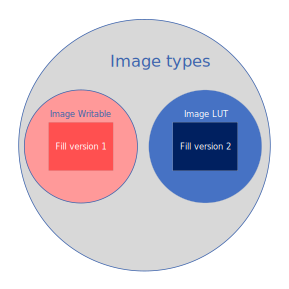
\includegraphics[width=.5\linewidth]{../figures/fill_version_diagram}
%   \caption{Diagram of the two versions of the fill algorithm.}
%   \label{fig:fill.version.diagram}
% \end{figure}

To implement a basic image algorithm such as \texttt{fill} there really are two distinct ways of writing it. For the set
of images type whose data type is encoded into each pixel, one must traverse the image and set each pixel's color to the
new one. However, for the set of images type whose data type is encoded in a look-up table, one only has to traverse the
look-up table to set each color to the new one. This translates into two distinct algorithms shown
in~\cref{fig:traverse.vs.LUT}. We can represent the diagram outlining that those two algorithms are two distinct
versions in~\cref{fig:image.version.vs.specialization}.

\begin{figure}[htbp]
  \centering
  \subfloat[Writable image fill algorithm]{
    \(fill(I, v)\colon \forall{p}\in\mathcal{D}, I(p) = v\)
  }
  \hfil
  \subfloat[Image LUT fill algorithm]{
    \(fill(I, v)\colon \forall{i}\in I.LUT, i = v\)
  }

  \caption{Comparison of implementation of the \texttt{fill} algorithm for two
    families of image type.}
  \label{fig:traverse.vs.LUT}
\end{figure}

More generally, we consider that the set of image type is formed of several subsets of image types. In the example there
are two subsets: images whose pixels are writable and images whose data type are ordered in a look-up table. \emph{For
  each one of these subsets, if there is a way to implement an algorithm then we have a \emph{version} of this algorithm}.

Sometimes, it is possible to take advantage of a property on a particular image set, that may be correlated to an
external data, to write the algorithm in a more efficient way. When those properties are linked to the types, it is
called algorithm \emph{specialization}~\parencite{jarvi.2006.specialization-article}. For instance, when considering a
dilation algorithm, if the structuring element (typically the disc) is decomposable then we can branch on an algorithm
taking advantage of this opportunity: decompose the dilation disc into small vectors and apply each one of them on the
image through multiple passes. The speed-up comparing to a single pass with a large dilation disc is really significant
(illustrated in~\cref{fig:gen.bench.square.disc}). The code in~\cref{fig:dilation.specialization.alg.diagram} illustrate
how an algorithm can be written to take advantage of the structuring element's decomposability property. The algorithm
will first decompose the structuring element into smaller 1D periodic lines. It will then recursively call itself with
those lines to do the multi-pass and thanks to known optimizations on periodic
lines~\parencite{vanherk.1992.localminmax}, it will be much faster. The dispatch diagram outlining the different
specialization of the dilation algorithm used is show alongside in~\cref{fig:dilation.specialization.alg.diagram}.

\begin{figure}[htbp]
  \begin{minipage}[l]{0.48\linewidth}
    \begin{minted}{C++}
template <Image Img, StructuringElement SE>
auto dilate(Img img, SE se) {
  if (se.is_decomposable()) {
    lst_small_se = se.decompose();
    for (auto small_se : lst_small_se)
      img = dilate(img, small_se) // Recursive call
    return img;
  } else if (is_pediodic_line(se))
    return fast_dilate1d(img, se) // Van Herk's algorithm;
  else
    return dilate_normal(img, se) // Classic algorithm;
}
\end{minted}
  \end{minipage}
  \hfill
  \begin{minipage}[r]{0.48\linewidth}
    \centering
    \includegraphics[scale=0.5]{../figures/dilation_specialization_diagram}
  \end{minipage}
  \caption{Dilate algorithm (left) with decomposable structuring element and its specialization diagram (right).}
  \label{fig:dilation.specialization.alg.diagram}
\end{figure}

The~\cref{fig:image.version.vs.specialization} shows how an algorithm specialization may exist in a set of algorithms
version. In this figure there exists a specialization of algorithms when it is known that the data buffer has the
following property: its memory is contiguous. This implies that, for example, an algorithm like \texttt{fill} can be
implemented using low level and fast primitives such as \texttt{memset} to increase its efficiency.

\begin{figure}[htbp]
  \centering
  \subfloat[Different versions of \emph{fill} algorithm]{
    \includegraphics[width=1.9in]{../figures/image_version}
  }%
  \hfil
  \subfloat[Specialization existing within a version]{
    \includegraphics[width=2.9in]{../figures/image_version_specialization}
  }%
  \caption{Set of algorithm version (a) and its specialization existing within a version (b).}
  \label{fig:image.version.vs.specialization}
\end{figure}

Making a full inventory of image types is not possible as there are many families of image types, each family may
intersect with each other, images may have some particular properties at some points, those properties may appear in
several families of image types. We can nonetheless cite a few to illustrate our points. There exists image-type whose
values are cubical complexes~\parencite{ziou.2002.cubical-complex} or layered as hexagonal or triangular grid instead of
square grids (such as meshes), that are represented as graphs~\parencite{meyer.2009.ismm}, etc. All of those interleaves
with different research areas (computer vision for meshes, topological classification for complex
cells~\parencite{movn.20.cviu,allili.2001.cubical}, graph theory and hierarchy for image
graphs~\parencite{carlinet.2014.tip,carlinet.2015.tip,perret.2019.higra}). Finally, this image type inventory does not
help when it comes to designing an image processing library. Instead, what helps is making an inventory of image
processing algorithms as well as what properties those algorithms can leverage to speed up their execution.

By making the inventory of image processing algorithms (limited to mathematical morphology), we distinguish three main
types of image processing algorithms. The first one are the pixel-wise algorithms. Those algorithms are the basic
pixel-wise transformation. They are the base of any image processing toolkit. Indeed, being able to extract the green or
red color channel of an image is mandatory. Thresholding as well as the previously seen gamma correction are such
algorithm. The second one are the local algorithms. Those algorithms perform transformations by considering all the
neighboring pixels around a given pixel. In order to operate, those algorithms need additional data in the form of
image's extension (defining border's behavior) and structuring element (disc, rectangle around the considered pixel).
Such algorithms are widely used in mathematical morphology. Dilation, erosion, closing, opening, gradient, rank filter
are all local algorithms, as well as stencil-type algorithms such as union-find, max-tree or skeletonize. Finally, the
third set of image processing algorithms is the global one. This set contains algorithms where computing the current
pixel requires to knowledge about what was previously computed for the previous pixels. Chamfer distance transform,
labeling, watershed, hierarchy structures related algorithms are in this category.


\section{Generic aspect of algorithm: canvas}
\label{sec:canvas}

Genericity is always referred to with this sentence \blockquote{write once, work for every type, run everywhere}.
However, very quickly we learned that the \emph{run} aspect can be a combination of:
\begin{itemize}
  \item as fast as possible on a single CPU unit;
  \item as fast as possible on thanks to using many CPU units;
  \item as fast as possible on thanks to using many GPU units;
  \item as fast as possible on thanks to using many computers (cloud) and their CPU/GPU units.
\end{itemize}
How do we decide what is the most efficient way to do? There is no simple answer to this question, but we can start by
studying the morphology of algorithms with two goals in mind: (i) find what can be parallelized/distributed and (ii)
find one or several algorithms' abstraction. Indeed, in image processing there are a lot of common patterns when one
looks at algorithms implementations, the most famous being \emph{for all pixels of an image, do something to each
  pixel}. But there are other more high-level similarities that we can leverage to have more generic algorithm. Let us
first study the different programmatic model there are commonly used to process images.

\FIXME{Rework these 3 paragraphs}

\paragraph{The pipeline} It is the classic way of doing the work. It consists of an imbrication of different operators
(algorithms) taking as input one or several images, maybe additional data as well (such as labels, adjacency map, etc.)
in order to process the data \blockquote{from left to right}. The result will show at the end of the pipeline and the
optimization opportunities are located inside the smaller operators and in the form of correctly managing data (no
useless copies, locality, etc.)

\paragraph{Kernels and tiling} They are the trendy way of the last decade. It consists in breaking the original image
into small tiles in order to feed those tiles into a massively multicore GPU (via CUDA,
Halide~\parencite{ragankelley.2013.halide}). Processing will happen concurrently on those core, but it is costly to swap
contents inside those GPU from the RAM memory. It's then preferred to design pipeline for those tiles so that the work
directly happens on each core to minimize the number of back and forth copies from the RAM.

\paragraph{Cloud computing} It is a huge deal in image processing these last years as well, especially used in Deep
learning applications. Deep neural networks are usually executed on cluster of computer through network (cloud) and thus
are leveraging combinations of successive \emph{MapReduce}~\parencite{dean.2008.mapreduce} under the hood. They can also
be offloaded onto or local available computers, or directly locally available GPU hardware thanks to frameworks that are
dynamically dispatching the workload (such as
Tensorflow/Keras~\parencite{tensorflow.2015.whitepaper,chollet.2015.keras,gulli.2017.deep},
PyTorch~\parencite{paszke.2019.pytorch}, etc.).

In every case there is a notion of pipeline where the user pipe algorithms into each others in order to achieve a
result. Those algorithms can leverage all the heterogeneous resources (cloud, GPU, CPU) they can to \emph{map} the input
data. Algorithms will then finally aggregate the results (\emph{reduce}) to output them into another algorithm, or save
them, or display them. It is important to dissociate the route the data will go through and the processing pipeline
logic. Both have their own specificities. In this thesis, we make a parallel, at small scale, between processing
pipeline logic and image processing algorithms. First let us study two basic algorithms: dilation and erosion. The
Python code of such algorithm is naively be given in~\cref{code:erode.dilate}.

\begin{figure}[htbp]
  \centering
  \subfloat[Dilation]{
    \includegraphics[width=1.7in]{../figures/dilation_code}
  }%
  \hfil
  \subfloat[Erosion]{
    \includegraphics[width=1.7in]{../figures/erosion_code}
  }%
  \caption{Dilate vs. Erode algorithms.}
  \label{code:erode.dilate}
\end{figure}

The algorithms are almost written the same way. The only change is the operation \emph{min} and \emph{max} when
selecting the value to keep. As such, we can easily see a way to factorize code by passing the operator as an argument.
The algorithms can then be rewritten as shown in~\cref{code:erode.dilate.factorized}. In this last example, we have one
piece of code which is in charge of abstracting the way an image is traversed: it is the canvas. We also have other
pieces of code which carry the logic of the operations, calling the canvas and providing the logic to apply from within
the canvas. This way of decomposing the code offers the opportunity of writing more specific heterogeneous logic for the
traversing code so that the other parts of the code that carry the operator logic remains unaware and unburdened of
possible implementation details.

\begin{figure}[htbp]
  \centering
  \subfloat[Local algorithm with custom operator]{
    \includegraphics[width=3.28in]{../figures/local_op_code}
  }%
  \vfil
  \smallskip
  \subfloat[Dilation (delegated)]{
    \includegraphics[width=1.64in]{../figures/local_op_dilation_code}
  }%
  \hfil
  \subfloat[Erosion (delegated)]{
    \includegraphics[width=1.64in]{../figures/local_op_erosion_code}
  }%
  \caption{New Dilate vs. Erode algorithms.}
  \label{code:erode.dilate.factorized}
\end{figure}

\subsection{Taxonomy and canvas}
\label{subsec.taxonomy.canvas}

This approach is very much compatible with the inventory of the algorithms we did in the previous~\cref{sec:image.set}.
Indeed, for the point-wise family of algorithms, it is hardly an issue as they can all be written in terms of
views~\cref{chap:image_views}. For the second family, which consists in all the local algorithm, they may be abstracted
behind an algorithm canvas where the user provides the work to do at each point of the algorithm. For instance, a single
pass local algorithm will always have shape given in~\cref{code:local.algorithm.canvas}. Finally, for third family which
consists in all the algorithm that propagate their computation while traversing the image. It is way less easy to
provide an algorithmic canvas as each algorithm has its own way to propagate changes curing its computation.

\begin{figure}[htbp]
  \centering
  \begin{minted}[linenos,xleftmargin=17pt,gobble=2]{python}
  def local_canvas(img, out, se):
    # do something before outer loop
    for pnt in img.points():
      # do something before inner loop
      for nx in se(pnt):
        # do something inner loop
      # do something after inner loop
    # do something after outer loop
  \end{minted}

  \caption{Local algorithm canvas.}
  \label{code:local.algorithm.canvas}
\end{figure}

This canvas can be customized to do a specific job, especially at the lines 2, 4, 6, 7 and 8. The user would then
provide callbacks and the canvas would do the job. This is especially useful when knowing that the canvas would handle
the border management (the user would provide a handling strategy like mirroring the image or filling it with a value).
The canvas would also take advantage of optimization opportunities (such as the decomposability of a structuring
element) that the user would probably forget, or not know, when first writing his local algorithm. Another advantage is
the opportunity to do more complex optimization such as parallelizing the execution or offloading part of the
calculation on a GPU. More generally, all optimization done through heterogeneous computing would be available by
default even if the user is not an area expert.

Despite all these advantages, one big disadvantage is the readability of the algorithm user-side. For instance, the
dilation algorithm is rewritten in~\cref{code:local.algorithm.dilate}.

\begin{figure}[htbp]
  \centering
  \begin{minted}{python}
def dilate(img, out, se):
  do_nothing = lambda *args, **kwargs: None

  def before_inner_loop(img, out, pnt):
    out(pnt) = img(pnt)

  def inner_loop(ipix, opix, nx):
    out(pnt) = max(out(pnt), img(nx))

  local_canvas(img, out, se,
    before_outer_loop = do_nothing,
    before_inner_loop = before_inner_loop,
    inner_loop        = inner_loop,
    after_inner_loop  = do_nothing,
    after_outer_loop  = do_nothing
  )
  \end{minted}

  \caption{Local algorithm canvas.}
  \label{code:local.algorithm.dilate}
\end{figure}

This way of thinking algorithms is far less readable than the classic way. The user does not see the loops happening,
and it can become very messy when several passes are happening (closing, opening, hit or miss, etc.)


\subsection{Heterogeneous computing: a partial solution, canvas}
\label{subsec:heterogeneous}

One of the key aspect driving genericity is performance. We still have the following mantra: \blockquote{write once,
  work for every type, run everywhere}. However, when considering the \emph{run} aspect, one has a lot to do. Indeed,
nowadays, leveraging the available resources to their maximum is long-standing issue. There are many ongoing works on
the subject, such as SyCL~\parencite{brown.2019.heterogeneous,wong.2019.heterogeneous} which is a standard for
heterogeneous computing model edited by Kronos. This standard currently has four implementations: Codeplay's
ComputeCpp~\parencite{codeplay.2021.computecpp}, Intel's LLVM/clang implementation~\parencite{intel-llvm.2021.sycl},
triSYCL~\parencite{xilinx.2021.triSYCL} led by Xilinx and hipSYCL~\parencite{aksel.2020.hipsycl} led by Heidelberg
University. There also exists smaller libraries such as Boost.SIMD~\parencite{esterie.2014.boostsimd} or even
VCL~\parencite{fog.2013.vcl} for easing how to write SIMD code. After taking some distance to study the subject, we can
infer that there are three main aspects to consider when optimizing performance.

The first one, the most important one is the algorithm to use in function of certain set of data. This aspect is covered
by the C++ language and its built-in genericity tool: template metaprogramming. Indeed, we select the most optimized
algorithm for a particular set of data.

The second one is the ability for the code to be understood by the compiler so that it can be further optimized during
the generation of the binary. Indeed, when compiling for the native architecture of a recent processor, one can use the
most recent assembly instructions to use wide vectorized registries (AVX512). The use of a recent compiler also brings
the help much needed.

Finally, the third aspect is not as trivial as the first two ones. It consists in studying the structure of an algorithm
to allow distributed computation. It also consists in studying the different architectures to select the most efficient
algorithm for a given architecture. Sometimes algorithm are friendly to be distributed on several processing units that
compute a part of the result concurrently. This is what we call parallelism. There exists several ways to take advantage
of parallelism. First there is the use of several CPU units on the host computer. Then there is the use of GPU units
working in combination with the CPU units to take advantage of the massive amount of core a graphic card can provide.
Finally, there is the use of cloud computing which consists in using several ``virtual'' computers, each of them
offering of CPU and GPU units in order to compute a result. One should be aware that each time we introduce a new layer
of abstraction, there is a cost to orchestrate the computation, send the input data and retrieve the results. It is thus
very important to study case by case what is needed. Some solutions exist that abstract away completely the hardware
through a DSL~\footnote{Domain Specific Language} such as Halide~\parencite{ragankelley.2013.halide}: the DSL compiler's
job will be to try very hard to make the most out of both the available (or targeted) hardware and the code. Those
solutions are not satisfactory for us as we want to avoid DSL and remain at code level. We are not developing a
compiler: we are working with it.

There is one true issue when studying parallel algorithm: it is whether they can be parallelized or not. Not all
algorithms can be parallelized. Some just intrinsically cannot, typically, algorithms that immediately need the result
at the previous iteration to compute the next iteration. There may exist specific ways to re-arrange a specific
algorithm, for instance, taking advantage of some algebraic property, in order to rewrite it in a parallelizable way,
but it is not trivial (on a per-algorithm basis), and not generic. As such, it is out of the scope of this thesis. What
interest us are the algorithms whose structure is an accumulation over a data type that can be defined as a monoid. We
assert that every algorithm that can be rewritten as an accumulation over a monoid can be parallelized and/or
distributed. This model that consists in distributing computation like an accumulation over a monoid data structure is
also call the map-reduce. This model has two steps: the distribution (map) and then the accumulation (reduce).

The map step will dispatch computation on subunits with small set of data. The reduce step will retrieve and accumulate
all those resulting data, as soon as they are ready.

The accumulation algorithm has this form:
\begin{minted}[linenos]{C++}
  template <class In, class T, class Op>
  auto accumulate(In input, T init, Op op)
  {
    for(auto e : input)
    {
      init = op(init, e);
    }
    return init;
  }
\end{minted}

The loop line 4 can be split into several calculation units which are going to be distributed, and then be accumulated
later once the units have finished their computation.

The issue left here is the monoid. What exactly is a monoid here? A monoid is a data structure which operates over a set
of values, finite or infinite. This data structure must provide a binary operation which is closed and associative.
Finally, this data structure must also provide a neutral element (aka the identity). Some trivial monoids comes to mind:
\begin{itemize}
  \item \emph{boolean}. For binary operation ``and'', identity is ``true'' whereas for binary operation ``or'', identity
        is ``false''.
  \item \emph{integer}. For binary operation \(-\) and \(+\), identity is \(0\) whereas for binary operation \(*\) and
        \(/\), identity is \(1\).
  \item \emph{string}. For concatenation, identity is empty string.
  \item \emph{optional} value (also known as monadic structure in Haskell programming language).
\end{itemize}
There are many more monoids, less trivial but very handy, such as the unsigned integer/max/0 set and the signed
integer/min/global max set.

This theory is extremely beneficial to image processing as the most commonly used algorithms, the local algorithms, can
all be written in the form of an accumulation over the pixels of an image. The fact that finding an identity for the
operation processed by the algorithm is often quite trivial led us to the idea of canvas. A canvas is a standard way to
write an iteration over an image which abstracts the underlying data structure. A canvas is a tool for the user to
provide its computation model based on events such as: \blockquote{entering inner loop} or \blockquote{exiting inner
  loop}. The user can then provide its operations as if he was writing his algorithm himself (restricted to the
accumulation model). As the maintainer of the library provides the canvas of execution, he can know also make change to
take advantage of it. For instance, computing a CUDA kernel at one point and dispatching it on GPU units is totally
within scope and transparent for the user of the library. Although there is a caveat: rewriting our algorithm in an
accumulation form and chunking it in fragments to feed to the canvas is definitely not intuitive. Indeed, we require our
user to change his way of thinking from the procedural paradigm to the event-driven paradigm. This approach is not new
and is used in other libraries such as Boost.Graph~\parencite{siek.2001.boostgraph} for similar purposes.
\citeauthor{dean.2019.monoids} talks about this recurring monoid pattern more in-depth in his
talk~\parencite{dean.2019.monoids}.

In image processing, we quickly come to identify \emph{local} algorithms, that reason about a group of pixel around a
given of coordinate. All those algorithms can be abstracted behind an accumulation of some sort, and they all have the
same morphology. Thus leading to the following abstraction:
\begin{minted}{C++}
template <class In, class Out, class SE, class T, class Op>
auto local_accumulate(In input, Out output, SE se, T init, Op op)
{
    auto zipped_imgs = ranges::view::zip(input.pixels(), output.pixels())
                                                  // (1)
    for(auto&& rows : ranges::rows(zipped_imgs))
    for(auto [px_in, px_out] : rows)
    {
        auto v = op(init, px_in.val());           // (2)
        for(auto nb : se(px_in))
        v = op(v, nb.val());                      // (3)
        px_out.val() = v;                         // (4)
      }
                                                  // (5)
  }
\end{minted}
From this code we can deduce some very useful and easy monoids by the following triplets:
\begin{itemize}
  \item \((type = boolean, operator = and, neutral = true)\) is a binary erosion
  \item \((type = boolean, operator = or, neutral = false)\) is a binary dilation
  \item \((type = unsigned integer, operator = max, neutral = 0)\) is a dilation
  \item \((type = signed integer, operator = min, neutral = global max)\) is an erosion
\end{itemize}

Now if we want to rewrite the \texttt{local\_accumulate} in an event driven paradigm, we need to identify the different
callbacks to expose our user on the call site. Especially, what will be of the callback parameters. There are five
callback events we have identified:
\begin{enumerate}
  \item before entering outer loop (no work is done)
  \item before entering inner loop (iteration over the pixel's neighbor)
  \item inner loop (actual operation to perform, result is accumulated)
  \item after exiting inner loop (iteration over the neighbor is over, what to do with the accumulated result?)
  \item after exiting outer loop (iteration over the image is over)
\end{enumerate}
\begin{minted}{C++}
template <class In, class Out, class SE, class T, class BeforeOuterLoopCB,
          class BeforeInnerLoopCB, class InnerLoopCB class AfterInnerLoopCB,
          class AfterOuterLoopCB>
auto local_accumulate(In input, Out output, SE se, T init,
                      BeforeOuterLoopCB bolCB, BeforeInnerLoopCB bilCB,
                      InnerLoopCB ilCB, AfterInnerLoopCB ailCB,
                      AfterOuterLoopCB aolCB)
{
  auto zipped_imgs = ranges::view::zip(input.pixels(), output.pixels()
  bolCB(input, output);                             // (1)
  for(auto&& row : ranges::rows(zipped_imgs))
    for(auto [px_in, px_out] : rows)
    {
      bilCB(px_out.val(), init, px_in.val())        // (2)
      for(auto nb : se(px_in))
        ilCB(px_out.val(), px_out.val(), nb.val())  // (3)
      ailCB(px_out.val(), init, px_in.val())        // (4)
    }
  aolCB(input, output)                              // (5)
}
\end{minted}
In this code, we can see that all the callbacks do not take the same type and/or number of parameters. Here is what the
call site would like if the user wants to perform a dilation:
\begin{minted}{C++}
local_accumulation(
  input,                                    // input image
  output,                                   // output image
  se,                                       // structuring element
  0,                                        // monoid's neutral element
  [](auto I, auto& O) { /* do nothing */ }, // (1) entering outer loop callback
  [](auto& o, auto init, auto in){          // (2) entering inner loop callback:
    o = std::max(init, in);                 // initialize with neutral element
  },
  [](auto& o, auto cur, auto nbh) {         // (3) inner loop callback:
    o = std::max(cur, nbh);                 // keep the local maximum
  },
  [](auto& o, auto init, auto in) {         // (4) exiting inner loop callback
    /* do nothing */
  },
  [](auto I, auto& O) { /* do nothing */ }  // (5) exiting outer loop callback
);
\end{minted}
It is very verbose and non-intuitive but hopefully, once the compiler optimize out the empty callbacks, the generated
code is as fast as a non-generic handwritten dilation.

\section{Library concepts: listing and explanation}
\label{sec:library.concepts}

Let us now delve into concepts related to the Image Processing area. Indeed, this domain has his specificities, and we
want to improve generic image processing library design by learning from our past experiments and working with new
techniques. The most basic usage of an image is the famous algebraic formula \(y = f(x)\) where \(y\) is a \emph{value}
generated by the \emph{image} \(f\) for the \emph{emph} \(x\). Aside from generating a value, an image can also
\emph{store} a value, as in \(f(x) = y\) where the value is \emph{assigned} to the image for a given point. Those
notions are the basis of our work and will drive the entire design.

\subsection{The fundamentals}

\label{subsec:fundamentals}

First, let us introduce the fundamental concepts deriving from the basis notion. The \emph{Value} concept is refined
into three distinct one in~\cref{table:concept.value.expressions}. There are the basic \emph{Value} but also the
\emph{ComparableValue} and the \emph{OrderedValue} which are useful when it comes to comparison or ordering algorithms.
The need behind those three concepts derives from the algorithms who need an ordering relation in order to function
properly. Most of mathematical morphology requires it. For instance, the ordering relation for a gray-scale image is
trivial whereas it is a field of research for colored (rgb-8bits) images.

The second fundamental brick is the concept of \emph{Point}, detailed in~\cref{table:concept.point.expressions} which is
a bit less open than the concept \emph{Value} as it must be totally ordered. Indeed, when accessing a value stored in an
image, whether it is about reading or mutating, it is important that there is only one accessed value.

Now we introduce an abstract way to represent this relation \(Value \times Point\): the Pixel. This is a well known
notion in image processing, and it represents a couple \((point, value)\). This abstraction layer is easy to move around
and contains facilities to read and mutate the pixel's value if possible. Indeed, not all pixels are able to mutate
their value. If the pixel is yielded by an image that only generates values on the fly then it cannot be mutated.
Henceforth, we introduce two new concepts: \emph{Pixel} and \emph{OutputPixel}
in~\cref{table:concept.pixel.definitions}. Those two concepts have a very similar interface described
in~\cref{table:concept.pixel.expressions}. They can both access the stored information: the point and the value. On top
of that, the \emph{OutputPixel} can mutate the value. When interacting with pixels, the user will want to be able to
write code as followed:
\begin{minted}{C++}
  auto pix = Pixel();     // Get a pixel
  auto val = pix.val();   // yield the pixel value
  auto pnt = pix.point(); // yield the pixel point
  pix.val() = 42;         // Assign a value
\end{minted}

We show how those three fundamental concepts interact with each other in the\\
diagram~\cref{fig:concept.pixel}.

\begin{figure}[htbp]
  \centering
  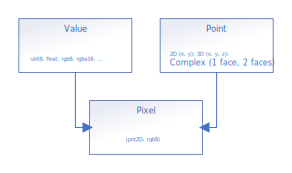
\includegraphics[width=.8\linewidth]{../figures/concepts/pixel}
  \caption{Pixel concept.}
  \label{fig:concept.pixel}
\end{figure}

Now we need a helper concept: the ranges.
Ranges~\parencite{niebler.2014.ranges,niebler.2018.ranges,niebler.2018.deepranges,niebler.2018.mergingranges} are a set
of concepts defined in the C++ standard library shipped with the ISO C++20 norm in 2020~\parencite{iso.2020.cpp}. They
allow the user to abstract away iterators to only iterate over one object: the range. This offers the user the
opportunity to migrate his source code from:
\begin{minted}{C++}
template <class IteratorBegin, class IteratorEnd>
void my_algorithm(IteratorBegin beg, IteratorEnd end)
{
  for(; beg != end; ++beg)
    // ...
}
\end{minted}
To:
\begin{minted}{C++}
template <class Range>
void my_algorithm(Range rng)
{
  for(auto e : rng)
    // ...
}
\end{minted}

In image processing, we refine further this concept by introducing multidimensional ranges (\emph{MDRange}). Indeed, in
image processing the user is used to write double loop to iterate over a bi-dimensional image. And abstracting away this
aspect under standard ranges induces performance loss. That is why we needed this concept to exist. A multidimensional
range can be split with a library function, \texttt{mln::ranges::rows(mdrng)} to fit the double-loop pattern and keep
its performance. This topic is tackle in-depth later in~\cref{subsec.range.traversing}. For now, let us consider
multidimensional ranges as an image processing extension for performance for the image traversing pattern. They are
defined in~\cref{table:concept.ranges.definitions} and their interface is the same as standard ranges, as seen
in~\cref{table:concept.ranges.expressions}. They are designed so that the user code looks like this:
\begin{minted}{C++}
  auto mdrng = MDRange(); // Get a multi-dimensional range of values
  auto rows = mln::ranges::rows(mdrng);
  for(auto row : rows) // double loop pattern
    for(auto val : row)
      // use(val)
\end{minted}

From an algebraic point of view, the definition of an image is not complete without considering a definition domain on
which it is defined. In image processing, the same rule applies. We cannot consider an image without considering the set
of points that are valid for this image. Henceforth, we must define the concept of \emph{Domain}
in~\emph{table:concept.domain.definitions}. The \emph{Domain} concept is refined into two sub-concepts which are
\emph{SizedDomain} and \emph{ShapedDomain}. This emphasis the chance of existence of possible infinite domain as
well as domains that may be defined over non-continuous intervals in space. This enables algorithms to require the
domain to have certain shape if needed. The domain behavior is described in~\cref{table:concept.domain.expressions}.

In practice, a domain is used to get information about the points constituting the image. Indeed, we can write code
like this:
\begin{minted}{C++}
  auto dom = Domain(); // Get a domain
  auto pnt = Point(..., ...); // Get a random point
  bool ret = dom.has(pnt); // Check wether the domain contains the point
  bool is_empty = dom.empty(); // Check wether the domain is empty
  auto dim = dom.dim(); // Yield the domain's dimension information
\end{minted}

We show how the concept \emph{Domain} flows from the previous concepts in the diagram shown in~\cref{fig:concept.domain}.

\begin{figure}[htbp]
  \centering
  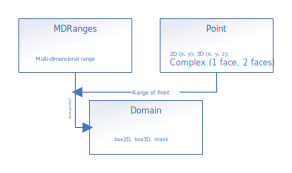
\includegraphics[width=.8\linewidth]{../figures/concepts/domain}
  \caption{Domain concept.}
  \label{fig:concept.domain}
\end{figure}

Now we have all the tools to introduce our main concept: \emph{Image}. As for \emph{Pixel}, we have the distinction over
image whose value can be mutated in a sub-concept named \emph{WritableImage}. These concepts are defined
in~\cref{table:concept.image.definitions.1}. In addition to this definition we can infer the behavior described
in~\cref{table:concept.image.expressions.1}. There are complicated requirements written in template metaprogramming code
and, in summary, they just require that the value types of the ranges returned by the member functions \texttt{pixels()}
and \texttt{values()} are the same as the value types declared in the parent image. In addition, we introduce two
facilities which are the member function \texttt{concretize()} and \texttt{ch\_value<V>()}. The first is a way to turn a
view into a concrete type. This will be seen more in-depth in~\cref{chap:image_views}. The last is a way to cast values
from one type to another. It forms a new image type whose underlying values will be returned after being converted to a
new value type. This last facility is extremely useful when one only wants to mutate the underlying type while keeping
all the other details about one type (such as the dimension). For instance, when working with labeling algorithm, we
know our algorithm will return an image similar to the input one except for the underlying type which will be the type
of the label. The following code shows how it is applied:
\begin{minted}{C++}
  using label_t = int; // label type

  template <class I> // Input image of type I
  auto my_labeling_algorithm(I input_image)
    -> image_ch_value_t<I, label_t> // Output image is Input image (I)
                                    // whose underlying type is label_t
  {
    // ...
  }
\end{minted}

We show the diagram building up the image concept from the previous concepts in~\cref{fig:concept.image}.

\begin{figure}[htbp]
  \centering
  \includegraphics[width=.8\linewidth]{../figures/concepts/image}
  \caption{Image concept.}
  \label{fig:concept.image}
\end{figure}


\subsection{Advanced way to access image data}
\label{subsec:advanced}

While being able to iterate over ranges of pixels or values is good, we are still lacking fundamental facilities to
access an element directly from the image. In order to solve this predicament, first we need to define the concept of
\emph{Index} in~\cref{table:concept.index.expressions} which we will use afterwards. This is a very simple concept that
encapsulate an integral value. This value can be negative as we want to be able to do negative indexing in case our
image has an extension, c.f.~\cref{subsec:advanced}. The first advanced tool is represented as an \emph{IndexableImage}.
An element can be accessed simply by providing its index number. This concept is defined
in~\cref{table:concept.image.definitions.2}. This introduces a simple behavioral pattern described
in~\cref{table:concept.image.expressions.2}. With this concept, we are able to write code as followed:
\begin{minted}{C++}
  auto ima = IndexableImage(); // Get an indexable image
  int k = 15; // Get an index
  auto val = ima[k]; // Get the element at the index
  ima[k] = 255; // Mutate the element at the index
\end{minted}
Being able to traverse an image through indexes is especially useful for algorithms that are aware of the number of
elements in the image. We chose to be flexible with our indexing method (i.e. allowing signed indexes) not to fall into
the same pitfall as the C++ core language~\parencite{stroustrup.2019.signed-unsigned-mess}. Indeed, requiring that the
type \texttt{std::size\_t} is unsigned lead to loads of issues, the first one being a conversion issue when writing a
simple for-loop. Solving these issues lead to the appearance of new member function \texttt{.ssize()} (for signed size)
and the new type \texttt{std::ptrdiff\_t} to store the result of a subtraction between two \texttt{std::size\_t}.
Furthermore, in our specific area (image processing), it may be well-defined to access a buffer with negative indexes
when, for instance, we are accessing the value of the extension of an image. This is why our indexes are signed.

Additionally, we want to be able to access a value by providing a point, the same way as in the algebraic definition
\(val = image(point)\). To do so, we introduce the concept of accessibility through \emph{AccessibleImage}. This concept
is defined in~\cref{table:concept.image.definitions.3}. This introduces new behavior that is described
in~\cref{table:concept.image.expressions.3}. We can notice facilities specifically including bound checking. Indeed, we
suppose, for fast access, that the user is always picking element from the image's domain, but it is possible to bound
check elements if needed on access for specific usages. With this concept, we are now able to write code as followed:
\begin{minted}{C++}
  auto ima = AccessibleImage(); // Get an accessible image
  auto p = Point(); // Get a point
  auto val = ima(p); // Get a value from a point
  auto val = ima.at(p) // Same with no bound checking
  auto pix = ima.pixel(p) // Get a pixel from a point
  auto pix = ima.pixel_at(p) // Same with no bound checking
  ima(p) = 42; // Assign a value from a point
  ima.at(p) = 42; // Same with no bound checking
  ima.pixel(p).val() = 42; // Assign a pixel value from a point
  ima.pixel_at(p).val() = 42; // Same with no bound checking
\end{minted}
Being able to traverse an image through points is especially useful for algorithms relying on restricting/expanding
definition domain that are exclusively yielding points.

Once we know that an image is both \emph{indexable} and \emph{accessible} we can introduce new behaviors (described
in~\cref{table:concept.image.expressions.4}) that we put behind the concept of \emph{IndexableAndAccessibleImage}
defined in~\emph{table:concept.image.definitions.4}. This behavior is related to accessing index from points and vise
versa. Indeed, it is possible to now write such code:
\begin{minted}{C++}
  auto pnt = ima.point_at_index(k); // Get the point from an index
  auto k = ima.index_of_point(pnt); // Get the index from a point
  // Get the index difference for a shift of delta_point
  auto delta_idx = ima.delta_index(delta_pnt);
\end{minted}

Additionally, it is useful, for propagating algorithms, to be able to traverse images in both a forward way and a
backward way. As it may not be possible for all images, this notion needs to be refined into a new concept
\emph{BidirectionalImage}. This concept is defined in~\cref{table:concept.image.definitions.5} and its behavior is
described in~\cref{table:concept.image.expressions.5}. Thanks to this concept, we are able to write code as followed:
\begin{minted}{C++}
  template <class I>
  my_algorithm(I input)
  {
    // forward pass
    for(auto pix : input.pixels())
      // ...

    auto backward = mln::ranges::views::reverse(input.pixels())
    for(auto pix : backward)
      // ...
  }
\end{minted}

Finally, we need a way, when possible, to iterate over a continuous data buffer for very fast and optimized calculation.
That is what the concept of \emph{RawImage} is for: an image whose data buffer can be accessed, as well as its mutable
counterpart, which are defined in~\cref{table:concept.image.definitions.6}. Having a raw image whose data buffer can be
accessed allow us to expose two more member function to access the data buffer and its strides for correct pointer
arithmetic. They behave as described in~\cref{table:concept.image.expressions.6}. This enables writing code as followed:
\begin{minted}{C++}
  auto ima = Image(); // Image of int
  const int* data = ima.data(); // Access the underlying buffer
  auto dim = ima.domain().dim(); // Get the dimension of the image
  // Retrieve information about strides
  auto strides = std::vector<std::ptrdiff_t>(0, dim)
  for (int i = 0; i < dim; ++i)
    strides[i] = ima.stride(i)

  // Now use data and strides to traverse the raw buffer
  // ...
\end{minted}

We show how those concepts are defined from one another in the diagram shown i~\cref{fig:concept.images}.

\begin{figure}[htbp]
  \centering
  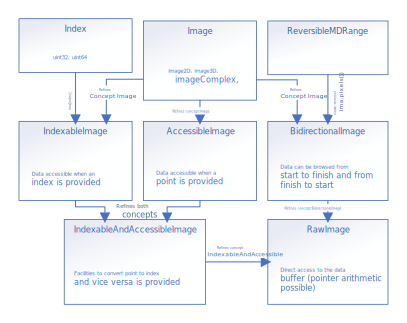
\includegraphics[width=.8\linewidth]{../figures/concepts/images_all}
  \caption{All images concepts.}
  \label{fig:concept.images}
\end{figure}


\subsection{Local algorithm concepts: structuring elements and extensions}
\label{subsec:local.se.ext}

From the beginning concepts are emerging from behavioral patterns extracted from algorithms. In image processing, there
is a family of algorithms called the \emph{local algorithms}. They work by considering a specific pixel as well as all
the pixels among a window having a specific shape centered in this first pixel. The window is called the
\emph{structuring element} and the pixels considered by this window are called the \emph{neighborhood}. This leads us to
introduce the concept of \emph{StructuringElement} which is defined in~\cref{table:concept.se.definitions}.

This concept is refined into three sub-concepts that are related to properties the structuring element can offer. Those
properties are:
\begin{itemize}
  \item decomposability: ability to split a complex structuring element into several smaller and simpler structuring
        element. There is an equivalence in behavior when the algorithm is recursively run for each smaller structuring
        element one after another, in a multi-pass way.
  \item separability: ability to split a complex structuring element into several smaller and simpler structuring
        element. There is an equivalence in behavior when the convolution is recursively run for each smaller
        structuring element one after another, in a precise order, in a multi-pass way.
  \item incremental: ability to tell the points that are added to or removed from the range when the structuring element
        is shifted by a basic displacement (e.g. for a \emph{2D point}, the basic displacement is \((0,1)\)). Usually
        used to compute attributes over a sliding structuring element in linear time.
\end{itemize}

\FIXME{Give examples}
%se::rect2D(pnt2D{2, 2}) :
%
%(0,0) (1,0) (2,0) (3,0) (4,0)
%(0,1) (1,1) (2,1) (3,1) (4,1)
%(0,2) (1,2) (2,2) (3,2) (4,2)
%(0,3) (1,3) (2,3) (3,3) (4,3)
%(0,4) (1,4) (2,4) (3,4) (4,4)
%
%decomposed in periodic lines:
%(0,2) (1,2) (2,2) (3,2) (4,2) 
%(2,0) (2,1) (2,2) (2,3) (2,4) 
%
%incremental
%(4,0) (4,1) (4,2) (4,3) (4,4) 
%
%decremental:
%(-1,0) (-1,1) (-1,2) (-1,3) (-1,4) 
%
%se::disc(radius=3, pnt2d{3, 3}) :
%                  (3,0)
%      (1,1) (2,1) (3,1) (4,1) (5,1)
%      (1,2) (2,2) (3,2) (4,2) (5,2)
%(0,3) (1,3) (2,3) (3,3) (4,3) (5,3) (6,3)
%      (1,4) (2,4) (3,4) (4,4) (5,4)
%      (1,5) (2,5) (3,5) (4,5) (5,5)
%                  (3,6)
%
%decomposed in periodic lines:
%(2,3) (3,3) (4,3) 
%(3,2) (3,3) (3,4) 
%(2,2) (3,3) (4,4) 
%(4,2) (3,3) (2,4) 

The behavioral for those concepts is described in~\cref{table:concept.se.expressions}. Being able to manipulate
structuring element allows us to write the following code:
\begin{minted}{C++}
  auto se = se::disc(.radius=3); // get a structuring element
  for(auto pix : ima.pixels())   // traverse image
    for(auto nb : se(pix))       // traverse neighboring pixels
      // ...
\end{minted}

Additionally, we introduce the concept of \emph{Neighborhood} in~\cref{table:concept.nbh.definitions}. This concept has
facilities to know what points/pixels are placed before or after another point/pixel inside the window of a specific
structuring element. It behaves as described in~\cref{table:concept.nbh.expressions}. This concept is useful when one
wants to only consider a certain part of the neighboring pixels within a structuring element. This offers the
opportunity to write the following code:
\begin{minted}{C++}
  auto se = se::disc(.radius=3); // get a structuring element
  for(auto pix : ima.pixels())   // traverse image
    for(auto nb : se.before(pix))// traverse neighboring pixels located before pix
      // ...
\end{minted}

And the last concept we need to introduce is the extension. Indeed, extension management is very important when dealing
with local algorithm as pixels on the border need to be processed too, and the behavior near the border of the image
must be defined and well-specified. There are several strategies when it comes to borders and extension. We refine
concept for each strategy we identified:
\begin{itemize}
  \item \emph{fillable}: fill the border with a specific value.
  \item \emph{mirrorable}: mirror the image as if there was an axial symmetry, with the border being the axis.
  \item \emph{periodizeable}: repeat the image, as if a modulo size was applied to the coordinates.
  \item \emph{clampable}: extend the value at the image's border into the extension.
  \item \emph{extent\_with}: used when tiling. It considers the current image as a sub-image of another bigger image and
        pick the extension values there.
\end{itemize}
Those concepts are defined in~\cref{table:concept.extensions.definitions} and their behavior is described
in~\cref{table:concept.extensions.expressions}. All those concepts allow us to introduce the final refined image
concepts: \emph{WithExtensionImage} as well as \emph{ConcreteImage} and \emph{ViewImage}. Those two last will be seen in
detail in the next~\cref{chap:image_views}. Those concepts are defined in~\cref{table:concept.image.definitions.7}.
Their behavior is described in~\cref{table:concept.image.expressions.7}. It is now possible to write the following code:
\begin{minted}{C++}
  template <class I, class SE>
  my_local_algorithm(I input, SE se) {
    // if the extension is large enough to function with the passed structuring element
    if(input.extension().fit(se)) {
      // ...
    }
  }
\end{minted}

We show how those three concepts (structuring elements, neighborhood and extension) interact with each other in the
diagram shown in~\cref{fig:concept.se_extension}.

\begin{figure}[htbp]
  \centering
  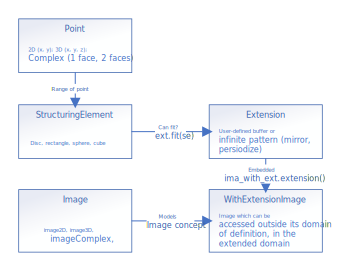
\includegraphics[width=.8\linewidth]{../figures/concepts/se_extension}
  \caption{Structuring element and Extension concepts.}
  \label{fig:concept.se_extension}
\end{figure}

Finally, we introduce a helper concept to centralize the detection of the ``writability'' of an image. Indeed, we do not
want the user to have to use the writable counterpart of each concept for each and every case. That is why we introduce
this final concept, \emph{OutputImage} in~\cref{table:concept.image.expressions.8}, that will tell the user if an image
is well-specified.

The correct way to use it is:
\begin{minted}{c++}
template <class Img>
requires RawImage<Img> && OutputImage<Img>
void my_algorithm(Img img) {
    // write data in img ...
  }
\end{minted}

\section{Summary}

In this chapter, we present that concepts are not designed after data structures but after algorithms. Indeed, a concept
consists in extracting a consistent behavioral pattern from a piece of code (algorithm) and name it to give him a
meaning. Through a simple but concrete example, we present in a didactic way how to extract concepts from an image
processing algorithm (gamma correction).

This chapter then proceeds to explain how, in theory, image types are related to each other. We present the set of
different image types and how algorithms exist in those sets, which introduce the notion of \emph{version} of an
algorithm. An algorithm will have different \emph{versions} for each image types set it supports. We distinguish it from
an algorithm \emph{specialization}, the latter being the ability to use an opportunity (related to a property) to make
an optimization and increase performances.

This chapter then proceed to describe the notion how algorithm canvas which is the result flowing from the taxonomy of
image processing algorithms. Indeed, there are three main algorithm families: the pixel-wise algorithms (binary
threshold), the local algorithms (dilation) and the global algorithms (Chamfer distance transform). We focus primarily
on local algorithms and how they can all be written through the same canvas of code. Indeed, for instance, the only
difference between a dilation and an erosion is the operator (max vs. min). We then discuss ways to exploit these canvas
to possibly solve heterogeneous computing issues.

Finally, this chapter introduces our first main contribution: a complete taxonomy related to the image processing area.
We first introduce fundamental concepts such as \emph{point}, \emph{pixel}, \emph{domain} and \emph{image}. We then
motivate and introduce advanced concepts related to images and the different way to access data (forward, backward
traversing, indexing, direct access to underlying buffer, \ldots). In the end, we introduce the concepts related to
orbiting notions such as \emph{structuring element}, \emph{neighborhood} and \emph{extension} (border management) which
are necessary to be able to work with local algorithms.

The next chapter will make use of the presented concepts to introduce the second main contribution of this thesis: the
\emph{image views}.


\cleardoublepage

\chapter{Image views}

\section{The Genesis of a new asbtraction layers: Views}

\section{Upgrading the way to design IP algorithms}

\subsection{Keeping properties}

\subsection{Lazy evaluation}

\subsection{Composability and piping}

\section{A practical example: border management}

\section{Performance discussion}


\cleardoublepage

\chapter*{Material about views}

\section*{Introducing range-based image traversing}
\label{sec.range.traversing}

Previously in Milena~\cite{levillain.2009.ismm} we had a very customized way of traversing images: macro-based. It aimed
at hiding the complexity of such a task while loosing as little performance as possible. For example, the dilation
algorithm was written this way:

\begin{minted}{c++}
  template<class I, class SE>
  mln_concrete(I) dilate(const I& f, const SE& se)
  {
    mln_concrete(I) g;
    initialize(g, f);
    mln_piter(I) p(f.domain());
    mln_qiter(SE) q(se, p);
    for_all(p) // for all p in f domain
    {
      mln_value(I) v = f(p);
      for_all(q) // for all q in se(p)
        if(f.has(q) and f(q) > v)
          v = f(q);
      g(p) = v;
    }
    return g;
  }
\end{minted}

In this code \texttt{mln\_concrete}, \texttt{mln\_piter}, \texttt{mln\_qiter}, \texttt{for\_all} and \texttt{mln\_value}
are all macros aiming at hiding the underlying complexity. Our goal is to replace those macros with existing C++ core
language code to improve the user experience as well as ease the maintenance, contribution and further improvement of
the library. Nowadays, a tool named range (and especially Eric Niebler's range-v3) allow seamless traversing of an
image. For instance, we can rewrite the above algorithm this way:

\begin{minted}{c++}
  template<class I, class SE>
  image_concrete_t<I> dilate(const I& f, const SE& se)
  {
    auto g = f.concretize();
    auto supr = accu::supremum<image_value_t<I>>();
    for(auto [f_px, g_px] : zip(f.pixels(), g.pixels()))
    {
      for(auto qx : se(f_px))
        supr.take(qx.val());
      g_px.val() = supr.result();
    }
    return g;
  }
\end{minted}

Here we have a much more efficient code that, in theory, enables compiler optimizations such as vectorization or inner
loops unrolling. But through benchmarking, we have learned that this solution doesn't mix well with the multidimensional
nature of images. The issue originates from the fact that we have no way to explicitly say in the code that the
multidimensional range is made of chunk of contiguous rows of memory. Indeed, for each element we have to compute an
index originating from potentially $N$ dimensions. This disables critical optimizations such as vectorization.

We solved this problem by augmenting range-v3's ranges with our own multidimensional ranges. Indeed, we only need to
have contiguity on the last dimension to provide the compiler code it can optimize. Which means that each for-loop that
traverses the whole n-dimensional image can be transformed into a double for-loop whose inner loop is guaranteed to be a
contiguous row. This way we have now an outer range as well as an inner range, as illustrated in
figure~\ref{fig.inner.outer.range}.

\begin{figure}[htbp]
  \centering
  \subcaptionbox{}{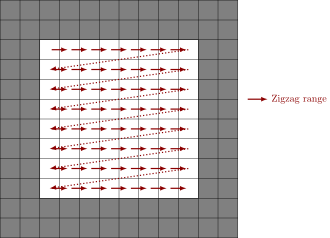
\includegraphics[width=.48\linewidth]{figs/linear_rng}}
  \subcaptionbox{}{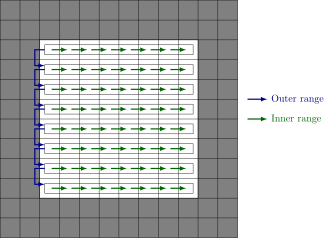
\includegraphics[width=.48\linewidth]{figs/segmented_rng}}
  \caption{Range-v3's ranges (a) vs. multidimensional ranges (b).}
  \label{fig.inner.outer.range}
\end{figure}

Thanks to this new design we can now rewrite our algorithm with a double for-loop for the image traversing. Hopefully it
stays really similar to what one would be used to when working with the classical two dimension image. As an example, we
can rewrite the dilation algorithm this way:

\begin{minted}{c++}
  template<class I, class SE>
  image_concrete_t<I> dilate(const I& f, const SE& se)
  {
    auto g = f.concretize();
    auto supr = accu::supremum<image_value_t<I>>();
    auto zipped_pixels = zip(f.pixels(), g.pixels());
    for(auto&& row : ranges::rows(zipped_pixels))
      for(auto [f_px, g_px] : row)
      {
        for(auto qx : se(f_px))
          supr.take(qx.val());
        g_px.val() = supr.result();
      }
    return g;
  }
\end{minted}

The highlight of this code is the usage a new tool: \texttt{ranges::rows} to bring out an inner range (contiguous) from
the multidimensional outer range.


\section*{Introducing Views}
\label{sec.views}

\subsection*{Practical genericity for efficiency: the Views}
\label{subsec.views}

Let us introduce another key point enabled by genericity and concepts: the \emph{Views}. A \emph{View} is defined by a
non-owning lightweight image, inspired by the design introduced in \emph{Ranges for the Standard
  Library}~\parencite{niebler.2014.ranges} proposal for \emph{non-owning collections}. A similar design is also called
\emph{Morphers} in \textsc{Milena}~\parencite{levillain.2009.ismm, geraud.2012.hdr}. \emph{Views} feature the following
properties: \emph{cheap to copy}, \emph{non-owner} (does not \emph{own} any data buffer), \emph{lazy evaluation}
(accessing the value of a pixel may require computations) and \emph{composition}. When chained, the compiler builds a
\emph{tree of expressions} (or \emph{expression template} as used in many scientific computing libraries such as
Eigen~\cite{guennebaud.2010.eigen}), thus it knows at compile-time the type of the composition and ensures a 0-overhead
at evaluation.

There are four fundamental kind of views, inspired by functional programming paradigm: \texttt{transform(input, f)}
applies the transformation $f$ on each pixel of the image \emph{input}, \texttt{filter(input, pred)} keeps the pixels of
\emph{input} that satisfy the predicate \emph{pred}, \texttt{subimage(input, domain)} keeps the pixels of \emph{input}
that are in the domain \emph{domain}, \texttt{zip($input_1$, $input_2$, \ldots, $input_n$)} allows to pack several pixel
of several image to iterate on them all at the same time.

\emph{Lazy-evaluation} combined with the view \emph{chaining} allows the user to write clear and very efficient code
whose evaluation is delayed till very last moment as shown in~\cref{fig.lazy} (see \cite{geraud.2018.gtgdmm} for
additional examples). Neither memory allocation nor computation are performed; the image $i$ has just recorded all the
operations required to compute its values.

\begin{figure}[htbp]
  \begin{minipage}[l]{0.48\linewidth}
    \begin{minted}{C++}
image2d<rgb8>  ima1 = /* ... */;
image2d<uint8_t> ima2 = /* ... */;

// Projection: project the red channel value
auto f = view::transform(ima, [](auto v) {
  return v.r;
});

// Lazy-evaluation of the element-wise
// minimum
auto g = view::transform(view::zip(f, ima2),
  [](auto value) {
    return std::min(std::get<0>(value),
             std::get<1>(value));
});
\end{minted}
  \end{minipage}
  \hfill
  \begin{minipage}[l]{0.48\linewidth}
    \begin{minted}{C++}
// Lazy-Filtering: keep pixels whose value
// is below < 128
auto h = view::filter(g, [] (auto value) {
  return value < 128;
}));

// Lazy-evaluation of a gamma correction
using value_t = typename Image::value_type;
constexpr float gamma = 2.2f;
constexpr auto max_val =
  std::numeric_limits<value_t>::max();
auto i = view::transform(h,
  [gamma_corr = 1 / gamma] (auto value) {
    return std::pow(value / max_val,
             gamma_corr) * max_val;
});
\end{minted}
  \end{minipage}

  \caption{Lazy-evaluation and \emph{view} chaining.}
  \label{fig.lazy}
\end{figure}

\noindent The tree of type resulting from this view chaining is illustrated by~\cref{fig.viewAST}.

\begin{figure}[htb]
  \includegraphics[height=2cm]{figs/viewAST.png}
  \caption{Abstract Syntax Tree of the types chained by the code above}
  \label{fig.viewAST}
\end{figure}

The concept of \emph{View} brought to us a fundamental issue when dealing with images: \blockquote{\emph{What is an
    image?}}. More precisely: should an image always be the owner of its data buffer? Should we have a shared ownership of
the data buffer between all the images using it? Then what happens when the data changes? The issue about the semantic
of an image is crucial but also very similar to the issue there is to differentiate a \emph{container} (such as
\texttt{std::vector}, that is to say the data buffer) and a \emph{view} on this container in the \emph{Ranges TS}.

From here we have considered two approaches. The first one is to have \emph{shared ownership} of the data buffer for the
image and its derived views. However this does not allow the differentiation between an already computed image and a
lazy image. To be able to make this differentiation is crucial in an \emph{Image Processing library} as we want to make
the most out of the data we already have and we do not want to compute data we do not need. Also, we cannot distinguish
when the \emph{copyability} property is required. This is the main reason why we did not adopt this approach.

The second one is to make the differentiation between a \emph{concrete image} which owns the data (like the standard
containers) and the \emph{views} that are lightweight cheap-to-copy objects. Not all \emph{concrete image} may be
\emph{copyable}, but all \emph{views} are. This is a very important property as it simplify greatly the reasoning when
performance is needed. It also enables us to have a library design similar to the standard library which the user is
familiar with and, why not, have standard algorithm and standard view work on our images types. All of these are the
main reason why we decided to adopt this design. Henceforth from now on the \emph{Image} concept is similar to the
\emph{View} concept from which we refines a \emph{ConcreteImage} concept that requires a specific behavior as it owns
data.


\vspace{1cm}

In~\cref{subsec.gen.concept}, we saw that what is truly important is the behavior: an algorithm will require its input
to be able to behave a certain way, and if those requirements are fulfilled, then the algorithm can be used with this
set of inputs. This enables non-standard type of image to be input in algorithms, providing they still behave correctly.
The way how we can check if the required behavior is satisfied is a new C++20 feature called \emph{concept} (the authors
show how to leverage them in~\cite{roynard.2019.rrpr}) that will not be presented in this paper. Additionally to
concepts, C++20 introduces a new library facility called \emph{ranges}~\cite{niebler.2018.deepranges} which includes a
non-owning lightweight container called \emph{views} whose design is very similar to that of \emph{morphers}, introduced
in Milena~\cite{levillain.2009.ismm,geraud.2012.hdr}. Views are completely transferable to the image processing world.
Also, views feature interesting properties that an image processing practitioner will find to his taste.

A view is a \emph{lightweight object} that behaves exactly the same as an image: let $V$ be a view of an image defined
on $\mathcal{D}$ then we have $\forall{p}\in\mathcal{D}, v = V(p)$. It can be a random generator that yields a random
number each time $V(p)$ is called; a proxy to the underlying image that records the number of times each pixel is
accessed in order, for instance, to compare algorithm performance; a projection to a specific color channel; applying an
automatic gamma correction; restricting the definition domain $\mathcal{D}$; and so on.

A view is a \emph{non-owning}, \emph{cheap-to-copy} lightweight object that basically only \emph{records an operation}
and stores a pointer to an image. For instance, let us consider the view transform defined as follow $v = transform(u_1,
  u_2, \cdots, u_n, f)$ where $u_i$ are input images and $h$ a n-ary function. $transform$ returns an image generated from
the other image(s) as show in~\cref{fig.view.threshold}. Also, we can see that the view itself does not own any image
but just stores pointers as well as the operation ($h$). This means that, for instance, modifying the original values of
the image(s) will impact the values yield by the view. Finally, as the view is cheap-to-copy, it features a pointer
semantic that help the practitioner passing around his images by copy to his algorithms without worrying about heavy
buffer copies in the background.

\begin{figure}[tbh]
  \centering
  \begin{minipage}{\linewidth}
    \includestandalone[mode=image, width=.9\linewidth]{figs/transform_thresholding}
  \end{minipage}
  \caption{An image view performing a thresholding.}
  \label{fig.view.threshold}
\end{figure}

Another key point of views is the lazy evaluation. When an image is piped through a view, no computation is done. The
computation happens when the practitioner requests a value by doing $val = V(p)$. The implications are multiples: an
image can be piped into several computation-heavy views, some of which can be discarded later on, it won't impact the
performance. Also, when processing large images, applying a transformation on a part of the image is as simple as
restricting the domain with a view and applying the transformation to this resulting sub-image.

Views will also try to preserve properties of the original image when they can. That means that views can preserve the
ability of the practitioner to, for instance, write into this image. This may be a trivial property to preserve when
considering a view that restrict a domain, but when considering a view that transforms the resulting values, it is not.
Let us consider the projection $h: (r,g,b) \mapsto g$ that selects the green component of an RGB triplet. When piping
the resulting view into, for instance, a blurring algorithm, the computation will take place in place thanks to still
having the ability to write into the image. A legacy way of obtaining the same result would have been to create a
temporary single-channel image consisting of the green channel of the original RGB image so that the temporary image
could then be blurred. Then one would have needed to copy the values of the temporary image back into the green channel
of the original image. The comparison between the legacy way and the in-place way of doing this computation is shown
in~\cref{fig.legacy.vs.view}.

\begin{figure}[tbh]
  \centering
  \subfloat[Legacy pipeline with copy]{
    \includegraphics[width=1.6in,align=t]{figs/blur_copy}
  }
  \hfil
  \subfloat[Modern pipeline with view]{
    \includegraphics[width=1.6in,align=t]{figs/blur_inplace}
  }

  \caption{Comparison of a legacy and a modern pipeline using \colorbox{lightgreen}{algorithms} and
    \colorbox{thistle}{views}.}
  \label{fig.legacy.vs.view}
\end{figure}

On the other hand, when considering the view $g: (r,g,b) \mapsto 0.2126*r+0.7152*g+0.0722*b$ that compute the gray level
of a color triplet (as shown in~\cref{fig.view.grayscale}), the ability to write a value into the image is not
preserved. One would need an inverse function that is able to deduce the original color triplet from the gray level to
be able to write back into the original image.

\begin{figure}[tbh]
  \centering
  \includegraphics[width=.98\linewidth]{figs/views/transform_grayscale}
  \caption{Usage of transform view: grayscale.}
  \label{fig.view.grayscale}
\end{figure}

\begin{figure}[tbh]
  \includestandalone[mode=image, scale=0.6]{figs/clip}

  \includestandalone[mode=image, scale=0.6]{figs/filter}
  \caption{Clip and filter image adaptors that restrict the image domain by a non-regular ROI and by a predicate that
    selects only even pixels.}
  \label{fig.view.clip}
\end{figure}

Following the same principle, a view can apply a restriction on an image domain. In~\cref{fig.view.clip}, we show the
adaptor \texttt{clip(input, roi)} that restricts the image to a non-regular \texttt{roi} and \texttt{filter(input,
  predicate)} that restricts the domain based on a predicate. All subsequent operations on those images will only affect
the selected pixels.

\begin{figure}[tbh]
  \includestandalone[mode=image, scale=0.6]{figs/pipeline}
  \caption{Example of a simple image processing pipeline.}
  \label{fig.view.pipeline}
\end{figure}

Views feature many interesting properties that change the way we program an image processing application. To illustrate
those features, let us consider the following image processing pipeline: (Start) Load an input RGB-8 2D image (a
classical HDR photography) (A) Convert it in grayscale (B) Sub-quantize to 8-bits (C) Perform the grayscale dilation of
the image (End) Save the resulting 2D 8-bit grayscale image; as described in~\cref{fig.view.pipeline}.


\begin{figure}[tbh]
  \begin{minipage}{\linewidth}
    \includestandalone[mode=image, scale=0.59]{figs/composition}
  \end{minipage}
  \caption{Algorithm vs image view composition.}
  \label{fig.view.comp}
\end{figure}

\textbf{Views are composable.} Chaining operations has always been a very important feature in image processing as well
as in software engineering in general (known object composition). Being able to weave simple blocks together into more
complex blocks in a way that the resulting block can still be treated as a simple block is a most wanted feature.
The~\cref{fig.view.pipeline} features an example of a pipeline using 3 basic operations \emph{Image} $\rightarrow$
\emph{Image}: a grayscale conversion, a sub-quantization and a dilation. It is important to note that we can consider
there is only one complex operation composed of 3 basic algorithms in which an image is piped. A view thus carries both
information about the image and the transformations. In~\cref{fig.view.comp} we show the distinction between the
composition of algorithms and the compositions of views which carry both the image and the transformations.

\textbf{Views improve usability.} The code featuring the pipeline in~\cref{fig.view.comp} can almost be implemented the
following way:
\begin{minted}{c++}
auto input = imread(...);
auto A = transform(input, [](rgb16 x) -> float {
    return (x.r + x.g + x.b) / 3.f; };
auto MyComplexImage = transform(A, [](float x)
    -> uint8_t { return (x / 256 + .5f); };
\end{minted}
When one is familiar to functional programming, it is quite easy to draw the parallel between \emph{transform},
\emph{map}, \emph{filter} and the sequence operators. Views are, in reality, higher-order functions built from an image
as well as the function(s) (operator or predicate) to apply for each pixel. It is not required to make the iteration
over each pixel of the image oneself, we just provide the function to morph the image into another one. The technique
used when composition several sequence operators is called \emph{currying}~\cite{hanus.1995.curry} in the functional
programming world.

\textbf{Views improve re-usability.} When looking at the code snippets above, one could see that they are simple though
not very re-usable. However, keeping the functional programming paradigm in mind, one can easily define new views just
by considering that a view is a \emph{higher-order function}. Then, as shown in~\cref{fig.view.highorder}, the primitive
\emph{transform} serves as the basis to build three new views: one that performs the summation of two images, one that
performs the grayscale conversion and one that performs the sub-quantization. All those three views can then be reused
afterwards\footnote{A more generic implementation could have been provided for these views for even more re-usability,
  but this is not the purpose here.}.

\begin{figure}
  \noindent
  \begin{minted}{c++}
auto operator+(Image A, Image B) {
  return transform(A, B, std::plus<>());
}
auto togray = [](Image A) { return transform(A, [](auto x)
  { return (x.r + x.g + x.b) / 3.f; };)
};
auto subquantize16to8b = [](Image A) { return transform(A,
  [](float x) { return uint8_t(x / 256 +.5f); });
};

auto input = imread(...);
auto MyComplexImage = subquantize16to8b(togray(A));
  \end{minted}

  \caption{Using high-order primitive views to create custom view operators.}
  \label{fig.view.highorder}
\end{figure}

\textbf{Views for lazy computing.} One fundamental point of views is that they embed the operation within themselves,
meaning that in~\cref{fig.view.highorder}, the creation of the views does not incur any computation. The computation is
delayed until the invocation of the \texttt{v(p)} expression. Also, the computation can be delayed quite far thanks to
the composition capability of views. In fact, a view is an image adaptor which actually is a \emph{template
  expression}~\parencite{veldhuizen.1995.expression, veldhuizen.2000.blitz}. Indeed, the \emph{expression} used to generate
the image is recorded as a template parameter. A view is represented by an \emph{expression tree}, as shown
in~\cref{fig.view.ast}.


\begin{figure}
  \null\hfill
  \begin{minipage}[b]{2cm}
    \includestandalone[mode=image, scale=0.8]{figs/view_ast}
  \end{minipage}
  \begin{minipage}[b]{5.5cm}
    \begin{minted}{c++}
Image f = ...; // grayscale
Image g = ...; // rgb16
Image out = subquantize16to8b(
              togray(g)) + f;
\end{minted}
  \end{minipage}
  \caption{View composition seen as an expression tree.}
  \label{fig.view.ast}
\end{figure}



\PLAGIAT{
  \textbf{Views for performance.} Consider a classical design where each operation of the pipeline is implemented on
  ``its own''. Each operation requires that memory be allocated for the output image, and also, each operation requires
  that the image be traversed. This design is simple, flexible, composable, but is not memory efficient nor
  computationally efficient. With the lazy evaluation approach, the image is traversed only once (when the dilation is
  applied) that has two benefits. First, there are no intermediate images so this is memory effective. Second, it is
  faster thanks to a better memory cache usage; processing a RGB16 pixel from the dilation algorithm directly converts
  it in grayscale, then sub-quantized it to 8-bits, and finally make it available. It acts \emph{as if} we were writing
  an optimal operator that would combine these operations.
}

\PLAGIAT{
  As an experiment, we benchmarked both pipelines on a 20MPix image RGB16 (random generated values) on a desktop
  computer i7-2600 CPU @ 3.40GHz, single-threaded\footnote{Experimentation code is available at
    \url{https://gitlab.lrde.epita.fr/mroynard/roynard.icip.2020.snippets}}. The dilation is done with a small 3x3 square
  structuring element using tiling for caching input values. The pipeline using views is about 20\% faster than the
  regular one (133 vs 106 ms). Note that views are also compatible with optimizations such as parallelization and
  vectorization.
}

\PLAGIAT{
  Background Subtraction: The background subtraction pipeline is used to detect changes in image
  sequences~\cite{opencv.bg_sub}. It is mainly used when regions of interest are foreground objects. The pipeline
  components include: subtraction, Gaussian filtering, threshold, erode and dilate, as shown
  in~\cref{fig.view.comp.sub_bg}.
}

\begin{figure}[tbh]
  \begin{minipage}{\linewidth}
    \includestandalone[mode=image, scale=0.59]{figs/pipeline_bg_sub_comp}
  \end{minipage}
  \caption{Background substraction pipeline using \colorbox{lightgreen}{algorithms} and
    \colorbox{thistle}{views}.}
  \label{fig.view.comp.sub_bg}
\end{figure}


\section*{From local algorithm to border management}
\label{sec.localgo.bm}

In image processing there are three main families of algorithms:
\begin{itemize}
  \item Point-wise algorithms: they process each value of the image, individually from each others (e.g.
        multiplication).
  \item Local algorithms: they process each value of the image, helped with the knowledge of the neighboring values
        catched in a window: the structuring element (e.g. convolution).
  \item Global algorithms: they propagate the changes downstream during the algorithm unrolling. Knowledge of previously
        computed values is required (e.g. chamfer distance transform).
\end{itemize}
Here we are interested in particular in local algorithms. The long recurring issue is about the behavior on the border
of the image. There are many ways of dealing with this problem. One is to allocate additional memory for the border and
paste values in it. Another is to check the bounds when looping over the neighbors. We can also decorate the image to
return a correct lazily computed value when accessing out-of-image's-bound value still inside the extension. The point
is: all these methods have advantages as well as disadvantages.

\subsubsection{Memory allocated border}
The border width is fixed at the image's creation and cannot be augmented without doing a reallocation. There is also a
cost when computing border's values (to fill it) which is proportional to the border's width and to the image's size. On
the other hand, the access time of a border value during the algorithm unrolling is as fast as a native access time
within the image itself. The last issue remaining would be that the border is not infinite. We cannot process a local
algorithm with a structuring element that does not fit in the extension. This method is especially adapted when there is
medium structuring elements with a known size which will yield a lot of out-of-image's bound accesses. When speed is
required, this method is a defacto standard.

\subsubsection{Bound checking}
Assuming there is no border and we are not allowed to access out-of-image's-bound values, a bound check is required when
accessing each values. Another way to do would be to decorate the facility that yields the neighbors of a pixel: do not
yield out-of-image's-bound pixels. This removes the need to bound check for each pixel's value which is relatively
faster. The caveats of this method are that it induces a slight slow down when yielding the pixel's neighbors from the
structuring element, and that it is not always viable: some algorithm do need to access values in an extension to
produce proper results.

\subsubsection{Image decoration}
The border is infinite and we make a view of our image to decorate it with the required extension. This method has the
advantage to \textit{always work}. Given any structuring element of any size, any algorithm will work. The disadvantage
is that we need to check for out-of-bound access at the image level, and lazily compute the value in case of
out-of-image's-bound access. The slowness induced is not negligible and should be weighted carefully.

\bigskip

It is important to note the very close relation between an image's domain (to perform out-of-bound checks), the
structuring element (notably its size) and the extension (its width). A user may require, for a specific set of those
three elements, to decorate the image, and/or the structuring element and/or to perform computation and/or reallocation.
To resolve this issue, we decided to provide the user with a new facility: the \textit{border manager} whose job is to
prepare a suitable couple (image and structuring element) given a set of configuration wanted by the user.

We designed the configuration to be configured from a given set of a policy and a method. We currently offer two
policies: native and auto.

\begin{itemize}
  \item Native: if the border is large enough: forward the image as-is to the algorithm to allow the fastest access
        possible. Otherwise, the border manager fails and halt the program.
  \item Auto: if the border is large enough: forward the image as-is to the algorithm to allow the fastest access
        possible. Otherwise, decorate the image with a view whose extension will emulate what is required by the algorithm
        with the given structuring element.
\end{itemize}

We also provide seven different methods to fill the values of our extension. It is important to note that not all the
methods are available for both policies. The policies are: none, fill, mirror, periodize, clamp, image and user.

\begin{itemize}
  \item None: enforce a policy where there is no border to use. The method cannot fail as it enforces the border to
        vanish. To enforce this method, the border manager decorate the structuring element in a view that checks the domain
        inclusion of each neighboring point.
  \item Fill: will fill the border with a specific value.
  \item Mirror: will mirror the image following an axial symmetry of image's edges.
  \item Periodize: replicate the image around, like a mosaic.
  \item Clamp: expand the value at the image's edge on the border.
  \item Image: assume all points out of the current image's domain are to be picked inside another image. A basic
        use-case is preparing tiles from a large image. The position of our image can be offset in the image acting as an
        extension which ease the ease of usage.
  \item User: Assume the user knows what he is doing and do not touch nor decorate the given image in any way. Both
        policies lead to the same behavior: check wether the structuring element fit and then forward the image as-is if it
        fits. An exception is raised if it does not.
\end{itemize}

As a consequence the usage of a local algorithm becomes very eased:

\begin{minted}{C++}
  // default border width is 3
  image2d<int> ima = {{0, 1, 0}, {0, 1, 1}, {0, 1, 0}};
  auto disc_se = se::disc{1}; // radius is 1
  auto bm = extension::bm::fill(0); // fill border with 0 with policy auto

  local_algorithm(ima, disc_se, bm); // will handle the border for you
\end{minted}

The border manager \texttt{bm} is set with the method fill (with value 0) and policy \texttt{auto} (wich is the default
policy). To use the policy \texttt{native}, one would write \texttt{extension::bm::native::fill(0)} instead.

\FIXME{put schemas showing different type of border management}

\FIXME{this can be intro of chapter}
Our work on bringing genericity to image processing through C++ template metaprogramming and concepts is presented
in~\parencite{roynard.2019.rrpr}. Continuing this previous work, we focused on the main goals of the library. First is the
zero-cost of traversing an image, overhauling the existing system which is macro-based. The new system presented in
section~\ref{part.image_views} is based on
range-v3~\cite{niebler.2014.ranges,niebler.2018.deepranges,niebler.2018.mergingranges}. Following, we will show in
section~\ref{part.image_views} a design around image's domain definition, extension and structuring element: how those
concepts link with each other when used to write local algorithms. Another objective of the library is the ease of use
and the binding with existing ecosystem, such as Python and NumPy. So we will present in
section~\ref{part.static_dynamic_bridge} our work about binding a generic C++ library to python. Finally, we will
discuss in section~\ref{part.image_and_algorithms_taxonomy} the issue of heterogeneous computing. We offer an avenue
around the idea of canvas algorithm that can be exploited to bring performance without being intrusive for the user.
Though it comes with its lot of disadvantage, such as a paradigm switch to event-driven programming.


\clearpage


\begin{itemize}
  \item origine, parallèle avec range-v3
  \item Value/Ref semantics des images
  \item Comment préserver les propriétés
  \item Évaluation paresseuse
  \item Composabilité/chaînage
  \item ...
  \item Performances + Bench
\end{itemize}

\cleardoublepage


\part{Bringing Generic programming to the dynamic world}
\label{part:dynamic.world}

\chapter{Static dynamic bridge}
\label{chap:static_dynamic_bridge}

%\section{Coexistence between the static world and the dynamic world}
%introduction

In the programming world, there are three main families of programming language~\parencite{kwame.2017.qualitative}.
There are the \emph{compiled} programming, such as C, C++, Rust or Go. There are also the \emph{interpreted} programming
languages, such as Python, PHP, Lisp or Javascript. Finally, there are the hybrid programming languages, such as Java or
C\#, that have a fast compilation pass that compiles the source code into an intermediate bytecode. Then, this bytecode
is interpreted via an interpreter on the host (runner) machine.


\section{Introducing the static and dynamic bidge}

Many studies have carried out to compare the advantages and disadvantages of each family of programming
languages~\parencite{prechelt.2000.comparison,kwame.2017.qualitative,boehm.1984.economics}. In this thesis we focus
mainly on comparing the burden that are shouldered by the maintainers and the end-user.


\subsection{Languages types}

\paragraph{Compiled languages} From the maintainer point of view, there is a lot of burden to shoulder. First is the
binary generation which can be problematic in itself. Indeed, to generate a binary, there are many steps, as illustrated
in~\cref{fig:static.dynamic.compiled.compiletime}. First the compiler does a pass to generate machine code for each
translation unit. There can be as many machine code as there are architecture and/or operating system supported. The
maintainer may want to support different operating systems (last two windows and OSX version, a handful linux or unix
distributions, maybe mobile phone portages). Each of this OS requires its own bundle. Additionally, the hardware may
change, or the maintainer may want to take advantage of some specific hardware when available (like vectorized SIMD
instructions such as SSE4, XOP, FMA4, AVX-512, etc.): this also requires the maintainer to multiply the number of
binaries he compiles and distribute. Finally, the linker resolves the dependencies of the program and assemble the final
binary. At that time the maintainer has to sort out how he wants to bundle the dependencies of his program. Should he
statically link them alongside the binary and distribute them, at the risk of having the size of his binary exploding?
Or should he state that the user has to install the dependencies on his system (via a package manager for instance) so
that the binary can run? The burden of handling the dependencies is then shifted to the end-user when installing the
program.

\begin{figure}[htbp]
  \centering
  \includegraphics[width=.6\linewidth]{figs/static_compiletime}
  \caption{Compiled languages: compile-time}
  \label{fig:static.dynamic.compiled.compiletime}
\end{figure}


Usually the package manager, such as \emph{apt}, \emph{yum} or \emph{pacman}, solves this transparently for the end-user
and the programs works "out-of-the-box" once installed, as illustrated in~\cref{fig:static.dynamic.compiled.runtime}.
The downside is that the maintainer has to publish many bundles of his package where he wants it to be available.

\begin{figure}[htbp]
  \centering
  \includegraphics[width=.6\linewidth]{figs/static_runtime}
  \caption{Compiled languages: run-time}
  \label{fig:static.dynamic.compiled.runtime}
\end{figure}

\paragraph{Interpreted languages} From the maintainer point of view, this is the ideal standpoint. It is easier to
distribute software via an interpreted language because only the source code and, a dependency tree and the assets are
released in the bundle. All the burden about resolving the dependencies and installing the framework to run the script
is shouldered by the end-user that is using the program. Indeed, as shown in~\cref{fig:static.dynamic.dynamic.pipeline},
everything happens at runtime. The main advantage of this approach is to build a very rich ecosystem as distributing,
maintaining and using programs is very easy once integrated in a package manager (often delivered alongside the language
SDK natively, e.g. pip for python). However, the most notable disadvantage is the performance which is explained by the
fact that the source code is not compiled into optimized assembly code ready to be executed by the computer. Instead,
the interpreter must do all the work in one go and very often this is slow (at least the first pass). Nowadays,
interpreters differentiate two use cases. One is opening the console interpreter from the command line and typing
commands to get the immediate interpreted results. This use-case usually do not provide heavy optimization because it is
likely the user is prototyping his script and thus does not need it in the first place. The second use case is when the
interpreter parses files and/or libraries as a whole. In this use-case, it is likely that the file will not change, but
they will be used a lot. It is then relevant to pay a pass to generate intermediate bytecode that can be interpreted
faster for the future passes onward. As an example, the Python programming language has several implementations:
CPython, PyPy, Jython or IronPython. CPython generate intermediate bytecode in \texttt{*.pyc} files while Jython
IronPython and PyPy embed a Just-In-Time (JIT) compiler to generate resp. JVM bytecode, CLR (.NET) bytecode, a large
variety of bytecode format.

\begin{figure}[htbp]
  \centering
  \includegraphics[width=.6\linewidth]{figs/dynamic_pipeline}
  \caption{Interpreted languages: run-time}
  \label{fig:static.dynamic.dynamic.pipeline}
\end{figure}

\paragraph{Hybrid languages} The burden is shared evenly between the maintainer and the user, while remaining minimal.
Indeed, languages such as Java or C\# are in this category. Those programming languages need a compiling pass which is
designed to be fast, so that the feedback loop while prototyping remains fast. The result of the compilation is bytecode
which is then executed on an hosting Virtual Machine (VM) that the user must install on his computer. The main
advantages of this solution are the portability and the small distributed binary size. Indeed, in theory, any machine
supporting the VM may also support the program. Also, the as the VM execute the bytecode and resolve system
dependencies, the distributed binary does not need to embed any system dependency. Finally, the user has the advantage
of running a compiled program which provides fast user experience. The goal of hybrid languages is to ally advantages of
both compiled and interpreted languages; no dependency management for the user, one small binary to distribute for the
maintainer, good execution performance, and fast feedback loop when prototyping (fast incremental compilation), while
minimizing the downsides; usually a garbage collector is working inside the VM to handle memory allocations and
de-allocations. In this regard, both Java and C\# manage to achieve this feat quite elegantly. In theory, VM can further
increase performances by implementing hot code detection which would compile the bytecode into native optimized machine
code. This area is still a field of research to this day (c.f. Java
HotSpot~\parencite{xie.improving,kotzmann.2008.hotspot,halli.2016.java-hpc}).


\subsection{Static and dynamic informations}

Compiles programming languages usually have poor support of introspection facilities. At best, static reflection is
available at compile-time, but dynamic reflection is not an option. The structure of the program does not change at
runtime. Some flexibility exists when delving into the area of hot-swapping dynamic libraries at run-time, however this
techniques drags alongside security-related issues that injecting possible foreign machine code into one's program may
generate.
Interpreted programming languages usually have very developed introspection facilities. Dynamic reflection at
runtime is possible and some language, such as Common Lisp, even go further by allowing the developer to mutate the
program Abstract Syntax Tree (AST) at runtime (macro). This allows very powerful integrations such as defining one's own
DSL as if it was part of the core language itself.
Hybrid programming languages usually offers very good static and dynamic introspection facility at both compile-time and
runtime, even if it means that runtime facilities will hurt performances. Also, those languages are usually designed to
be able to hot-swap code at runtime. It is then possible to have the application running, recompile part of the binary
of the application, replace the old running binary by the new compiled one, all the while the application is running.

The next important step is to classify what information is known at \emph{compile-time} (machine/bytecode code
generation): we call it \emph{static} information; and what information is known at \emph{runtime} (program execution):
we call it \emph{dynamic} information. In image processing, have the following static informations:
\begin{itemize}
  \item Image's value type (unit8, rgb8, complex, etc.),
  \item Image's dimension size (1D, 2D, 3D, etc.),
  \item Architecture of the hardware hosting the program (x86, ARM, PowerPC, GPU, etc.).
\end{itemize}

On the other hand, we have the following dynamic informations:
\begin{itemize}
  \item Image's actual values,
  \item Image's actual size,
  \item Architecture of the hardware hosting the program (x86, ARM, PowerPC, GPU, etc.).
\end{itemize}

We notice that the architecture hosting the program is both an information which is static and dynamic. This translates
the complexity of this information. Indeed, the maintainer needs to guess the array of architectures he wants to support
and generate binaries for them (static). Also, the program needs to detect at runtime (dynamically) on which hardware he
is running to possibly take advantage of it to increase performances. This is an area of research on its own called
heterogeneous computing~\parencite{wong.2019.heterogeneous,brown.2019.heterogeneous}.


\subsection{Introducing our hybrid solution}

Image processing communities like to have bridges with interpretable language such as Python or Matlab, to interface
with their favorite tools, algorithms and/or facilities. As an example, with Python, the module
NumPy~\cite{oliphant.2006.numpy} is a community standard which is heavily used. Henceforth, to broaden the usage of our
library, we should be able to provide a way to communicate between our library and NumPy. There is always a need for
genecity in both C++ and Python. Indeed, in C++ genericity is achieved via template programming, which is static,
whereas in Python genericity is achieved via duck typing, which is dynamic, as shown
in~\cref{fig:static.vs.dynamic.genericity}.

\begin{figure}[htbp]
  \centering
  \subfloat[C++ static genericity]{
    \includegraphics[width=2in]{figs/cpp_static_code}
  }
  \hfil
  \subfloat[Python dynamic genericity]{
    \includegraphics[width=2in]{figs/python_dynamic_code}
  }
  \caption{C++ Static (a) vs. Python Dynamic (b) genericity.}
  \label{fig:static.vs.dynamic.genericity}
\end{figure}

On the one hand, static polymorphism induces no indirection in the generated code as the type is known at compile-time.
It is then possible to generate optimized code for specific types. It is not possible to add a new supported type at
runtime as the code has already been compiled. On the other hand, the dynamic polymorphism implies that there will be
indirections when executing the code. Indeed, the code first needs to dispatch onto the appropriate function handling
the input types to perform the operation properly. Nevertheless, it is possible to add new supported type at runtime
without recompiling the library binary.

From the maintainer point of view, however, only distributing the C++ templated source code is a showstopper to the
usability of his library by a Python user, because he does not hand over binaries. Indeed, one caveat of using C++
template programming is that the C++ compiler cannot generate a binary until it knows which type (of image, of value)
will be used. But the maintainer does not know this information and the user (on Python's end) does not want to
recompile the generic library code each time he has another set of types to exercise against. From here, there are still
multiple ways to achieve our goal.

The first option is to embed and distribute, alongside the library, a JIT compiler whose job would be to generate the
binaries and bindings just as they are used. This solution brings speed (excluding the first run that includes the
compilation time) and unrestrained genericity. However it bounds both user and maintainer to the specificities of a
compiler vendor and loose platform portability.

Another option is to type-erase (dynamic polymorphism) our types to enables the use of various concrete types through a
single generic interface. This would translate into a class hierarchy whose concrete classes are the leaves (thus, whose
value-types and dimensions are known). This induces a non-negligible performance overhead but enables us to keep the
genericity and portability at the cost of maintaining the class hierarchy.

Type generalization can also be considered. It is possible to cast everything into a super-type that is suitable for the
vast majority of cases. For instance, we could say that we have a super-type \texttt{image4D<double>} into which we can
easily cast sub-types such as \texttt{image2D<int>} or \texttt{image3D<float>}. Of course we would loose the generic
aspect and induce non negligible speed cost. Although portability is kept.

And finally there is the dynamic dispatch. It consists in embedding dynamic information at runtime about types, and
dispatch (think of switch/case) to the correct facility which can handle those types. The obvious caveat is the cost of
maintenance induced by the genericity as we would have a number of possible dispatches that grow in a multiplicative way
with the number of handled types. Which is not very generic. On the other hand there is almost no speed loss and the
portability is guaranteed. Theoretical models exist that could bring solutions to lower the number of dispatcher to
write, such as multi-method~\cite{pirkelbauer.2010.multimethods}. Unfortunately they are currently not part of C++.

In Pylene we have chosen a hybrid solution between type-erasure and dynamic dispatch. The aim is to have a set of known
types for which we have no speed cost as well as continuing to handle other types to remain generic.
In~\cite{gossec.2019.pybind} we provide a facility to expose our generic code to Python. As seen in the previous
chapter, it is not possible to bind C++ source code to Python. We need to have a compiled binary implementing Python
binding (we chose Pybind11~\parencite{jakob.2017.pybind11}) in order to be able to call C++ code from Python. In order
to achieve the binding without sacrificing the genericity and the performances, we have designed a solution in two
steps. We do not want to provide an abstract interface that will resolve the calls to access data on the call-site via
virtual call because it would be very slow when the C++ code is executed. This would defeat the purpose of having to
rely on C++ in a first place. However, it is possible to convert an abstract class into an instantiated concrete generic
class whose template parameter are known. This requires, however, to enumerate all the possible cases. With modern C++,
it has become possible to design $n*n$ dispatch without gigantic switch-case clauses.


\section{Hybrid solution's first step: type-erasure}

The first step of our solution consists in designing a buffer class that holds all the informations about an image:
dimension, underlying type, strides and pointer to data buffer. This class is named \texttt{ndimage\_buffer}. When
interfacing with Python, it is necessary to convert the Python image which is a \texttt{NumpPy.array} into our image
type. The purpose of this buffer image is to holds all the information from the \texttt{NumpPy.array} to then
instantiate a concrete C++ type. The first pitfall here is due to a limitation from the abstraction interface used in
Python. Indeed, when using for instance \emph{Scikit-Image}, it is not possible to differentiate a 2D multichannel image
from a 3D grayscale image. Indeed, the image is always broken down to its most simple value and a 3D multichannel image
is turned into a 3-dimensional \texttt{NumpPy.array} containing 8-bits values, the last dimension contains only 3
elements at max but can theoretically contain more as there is no limitation from the used abstraction to prevent that.
A 3D grayscale image will be broken down into a 3-dimensional \texttt{NumpPy.array} containing 8-bits values, the last
dimension will contain many values as it is expected of a 3D-image. To prevent this confusion, there is a need to
explicitly say to the Python/C++ wrapper wether the image is multichannel or not. This information must be carried
through the \texttt{ndimage\_buffer} into C++ for a correct instanciation. This process is illustrated
in~\cref{fig:type-erased.buffer}.

\begin{figure}[htbp]
  \centering
  \includegraphics[width=.6\linewidth]{figs/type-erased_buffer}
  \caption{Bridge from Python to C++ via Pybind11 and a type-erased C++ class.}
  \label{fig:type-erased.buffer}
\end{figure}

From the point of view of a practitioner, the code on the call-site (python side) should be as follow:
\begin{minted}{python}
  from skimage import data
  import numpy as np
  import Pylena as pln # our python binding
  img = data.astronaut() # 2D-rgb8 image -> Numpy.array(ndim=3, dtype='uint8')
  pln_img = pln.ndimage(img, multichannel=True) # manualy point out multichannel information
  # use(pln_img) for any pln.<algorithm> exposed to Python
\end{minted}

From the point of view of the library implementer, the code to expose the binding looks like this one:
\begin{minted}{C++}
  #include "ndimage.hpp"
  #include <pybind11/pybind11.h>

  // Expose pybind module
  void init_class_ndimage(pybind11::module& m);
  PYBIND11_MODULE(Pylena, m) { init_class_ndimage(m); }

  // declare the conversion function
  namespace mln::py {
    mln::ndbuffer_image   ndimage_from_buffer(pybind11::buffer b, bool is_multichannel = false);
    pybind11::buffer_info ndimage_to_buffer(const mln::ndbuffer_image& img);
  }

  // expose the python ndimage class with the conversion from/to py::buffer (numpy.array buffer)
  void init_class_ndimage(py::module& m) {
    using namespace pybind11::literals;

    py::class_<mln::ndbuffer_image>(m, "ndimage", py::buffer_protocol(), "is_multichannel"_a = false)
      .def(py::init(
          [](py::buffer b, bool is_multichannel = false) {
              return ndimage_from_buffer(b, is_multichannel); }))
      .def_buffer(ndimage_to_buffer);
  }
\end{minted}

This code declares a new module named \texttt{Pylena}. It then declares a class named \texttt{ndimage} which is a bridge
to Python's \texttt{buffer\_protocol}. This \texttt{buffer\_protocol} is an abstraction to allow the usage of numpy's
array. Finally, the code declares that the class is convertible to and from the \texttt{buffer\_protocol} thanks to
provided callbacks. The code of those callbacks is as follow:

\begin{minted}{C++}
  // implement the conversion from Python to C++
  mln::ndbuffer_image ndimage_from_buffer(::py::buffer b, bool is_multichannel) {
    /* Request a buffer descriptor from Python */
    ::py::buffer_info info = b.request();

    std::ptrdiff_t      strides[16];
    int                 dims[16];
    int                 ndim = info.ndim - is_multichannel ? 1 : 0;
    int                 bpp  = info.itemsize;

    // convert the type information from Python to C++ (string to enum) for faster dispatch
    mln::sample_type_id st   = get_sample_type(info.format, is_multichannel);

    for (int i = 0; i < ndim; ++i) {
      dims[i]    = info.shape[ndim - 1 - i];
      strides[i] = info.strides[ndim - 1 - i];
    }

    if (strides[0] != bpp)
      throw std::runtime_error("Unsupported image stride along the last dimension.");

    // construct the type-erased image with all informations
    return mln::ndbuffer_image::from_buffer(
      reinterpret_cast<std::byte*>(info.ptr), st, ndim, dims, strides);
  }

  // implement the conversion from C++ to Python
  ::py::buffer_info ndimage_to_buffer(const mln::ndbuffer_image& img)
  {
    // return the python format of the underlying type, as well as information about multichanneling
    auto [ti, is_multichannel, channel_count, channel_stride] =
            get_sample_type_id_traits(img.sample_type());

    int ndim = img.pdim() + is_multichannel ? 1 : 0;

    std::vector<ssize_t> dims(ndim);
    std::vector<ssize_t> strides(ndim);

    for (int i = 0; i < ndim; ++i) {
      dims[i]    = img.size(ndim - 1 - i);
      strides[i] = img.byte_stride(ndim - 1 - i);
    }
    dims[ndim - 1]    = channel_count;
    strides[ndim - 1] = channel_stride;
    // construct the python buffer with all the information
    return ::py::buffer_info(img.buffer(), ti.size(),
            get_sample_type(img.sample_type(), is_multichannel), ndim, dims, strides);
  }
\end{minted}

This code forward informations about the buffer and handle the special case of multichannel images which Python treat
as 3D images.


\section{Hybrid solution's second step: multi-dispatcher (a.k.a. $\protect n*n$ dispatch)}

The second step of our hybrid solution is to dispatch the type-erased code to efficient generic code. The naive way of
doing so would be to include a gigantic switch-case clause in each algorithm implementation and dispatch to the correct
instantiated generic algorithm from there. Aside from being a nightmare to maintain, the size of those clause can grow
several fold depending on the cardinality of the generic implementation. For instance, for a generic dilation, there are
3 axis of cardinality: the underlying type, the dimension, the structuring element shape. In the case where the library
support 5 different structuring element shape, 10 underlying types and 6 dimension for the image, the switch-case
statement will have 300 clauses to dispatch. And each algorithm will have to dispatch. This solution is not viable,
defeat the purpose of genericity which is to write less code in the first place. We had to find a solution to have those
dispatch while keeping our code short and efficient. The idea we took to solve this problem comes from the design of a
C++ feature, the variant, and especially the visitor. We need to have a way to write the implementation of the algorithm
once while enumerating all the possible cases. Also, if possible, the list of supported types should be written once at
one place for maintenance purpose.

We then had the idea of writing a dispatcher. This dispatcher list all the supported types and call the given callbacks
forwarding the given arguments by instantiating a specific type. For instance, let us first expose the binary threshold
operator to Python. The Python call-site code will look like this:

\begin{minted}{python}
  img_grayscale = skimage.data.grass()
  pln.operators.binary_threshold(img_grayscale)
\end{minted}

On C++ side, we need to expose the function with this code:
\begin{minted}{C++}
  void init_module_operators(pybind11::module& m);

  mln::ndbuffer_image binary_threshold(::py::buffer buffer)

  void init_module_operators(::py::module& m) {
    using namespace pybind11::literals;

    m.def("binary_threshold", binary_threshold,
          "Perform a binary threshold.\n",
          "Input"_a);
  }

  PYBIND11_MODULE(Pylena, m) {
    /* ... */

    auto operators = m.def_submodule("operators", "Image processing operators.");
    init_module_operators(operators);
  }
\end{minted}

Now that our python submodule and that our \texttt{binary\_threshold} operator are declared, let us have a look to the
operator's implementation:

\begin{minted}{C++}
  mln::ndbuffer_image binary_threshold(::py::buffer buffer)
  {
    // grayscale image mandatory
    auto input = mln::py::ndimage_from_buffer(buffer);

    // dispatch along dimension (dimension is a valued template parameter, hence _v)
    return dispatch_v<binary_threshold_operator_t>(input.pdim(), input);
  }
\end{minted}

We have replaced the gigantic switch-case clause by a dispatcher templated by an operator. This operator will cast the
input image into the concrete generic type and call the fast generic algorithm on it. Let us have a look to what this
operator look like:

\begin{minted}{C++}
  // Operator templated by the dimension
  template <auto Dim>
  struct binary_threshold_operator_t {
    // Function templated by the image type
    template <typename Img>
    mln::ndbuffer_image operator()(Img&& img) const {
      // Cast to a grayscale (information known) of the correct dimension
      if (auto* image_ptr = std::forward<Img>(img).template cast_to<std::uint8_t, Dim>(); image_ptr)
        // call generic algorithm
        return mln::operators::binary_threshold(*image_ptr);
      else {
        std::runtime_error("Unable to convert the image to the required type.");
        return {};
      }
    }
  };
\end{minted}

This operator will attempt to cast the given image into a grayscale image of the correct dimension and then use the
resulting concrete type to pass it the fast generic \texttt{binary\_threshold} operator. Now let us have a look at where
the magic happen, at the dispatcher which list all the supported type.

\begin{minted}{C++}
template <template <auto> class V, typename... Args>
auto dispatch_v(std::size_t dim, Args&&... args) {
  switch (pdim) {
  case (1):
    return F<1>{}(std::forward<Args>(args)...);
  case (2):
    return F<2>{}(std::forward<Args>(args)...);
  case (3):
    return F<3>{}(std::forward<Args>(args)...);
  case (4):
    return F<4>{}(std::forward<Args>(args)...);
  case (5):
    return F<5>{}(std::forward<Args>(args)...);

  /* ... */

  case (0):
    [[fallthrough]];
  default:
    throw std::runtime_error("Unsupported dimension.");
}
\end{minted}

The dispatcher is instantiate the given type by the correct dimension number and then call the operator parenthesis
(function call) forwarding all the given parameters. In our case, it will instantiate the type
\texttt{binary\_threshold\_operator\_t<2>} and then call the function
\texttt{binary\_threshold\_operator\_t<2>.operator()(input)}, forwarding the input image to the underlying algorithm.

The main advantage of this approach is that all the supported features are to be listed only in one place, the
dispatcher, while any number of dispatcher can be piped to achieve the cardinality wanted. Let us push our example to
implement the mathematical morphology operator dilation. We now have two more generic axis to cover: the structuring
element shape and the underlying datatype. First, let us expose the operator to the Python code. Here is what the Python call-site look like:

\begin{minted}{python}
img_grayscale = skimage.data.grass()
rect = pln.se.rect2d(width=3, height=3)
pln.operators.dilate(img_grayscale, se)
\end{minted}

We need to expose the new structuring element's sub-module for usage in the dilation operator:

\begin{minted}{C++}
void init_module_se(pybind11::module& m);

void init_module_se(::py::module& m) {
  ::py::class_<mln::se::disc>(m, "disc").def(
      ::py::init([](float radius) { return mln::se::disc{radius}; }));

  ::py::class_<mln::se::sphere>(m, "sphere").def(::py::init([](float radius) {
    return mln::se::sphere{radius};
  }));

  ::py::class_<mln::se::rect2d>(m, "rect2d").def(::py::init([](int width, int height) {
    return mln::se::rect2d{width, height};
  }));

  ::py::class_<mln::se::rect3d>(m, "rect3d").def(::py::init([](int width, int height, int depth) {
    return mln::se::rect3d{width, height, depth};
  }));
}

PYBIND11_MODULE(Pylena, m) {
  /* ... */

  auto mse = m.def_submodule("se", "Structuring elements module.");
  init_module_se(mse);
}
\end{minted}

Now we need to expose the dilate function into the operator submodule:
\begin{minted}{C++}
// using std::variant
using se_t = std::variant<mln::se::disc, mln::se::sphere,
                          mln::se::rect2d, mln::se::cube>;

mln::ndbuffer_image dilate(::py::buffer buffer, const se_t& se)

void init_module_operators(::py::module& m) {
  /* ... */

  m.def("dilate", dilate,
    "Perform a morphological dilation.\n"
    "\n"
    "structuring element must be valid.",
    "Input"_a, "se"_a);
}
\end{minted}

We are all set to now implement the dilation operator. First, let us have a look at the underlying operator that will be
dispatched:

\begin{minted}{C++}
template <auto Dim, typename T>
struct dilate_operator_t {
  template <typename Img, typename SE>
  mln::ndbuffer_image operator()(Img&& img, SE se) const {
    if (auto* image_ptr = std::forward<Img>(img).template cast_to<T, Dim>(); image_ptr)
      return mln::dilation(*image_ptr, se);
    else {
      std::runtime_error("Unable to convert the image to the required type.");
      return {};
    }
  }
};
\end{minted}

Here we can see that we need a double dispatch. Also, the structuring element is no longer a variant and needs to be
dispatched before instantiating this operator. Finally, there is an issue here because there are two template parameters
and our dispatcher \texttt{dispatch\_v} does only handle one. We workaround this issue by writing another intermediate
operator dispatcher \texttt{dilate\_operator\_intermediate\_t} serving as trampoline that will partially instantiate the
final operator \texttt{dilate\_operator\_t} along the dimension template parameter to feed it to the last dispatcher,
\texttt{dispatch\_t}:

\begin{minted}{C++}
template <auto Dim>
struct dilate_operator_intermediate_t {
  template <typename Img, typename SE>
  mln::ndbuffer_image operator()(Img&& img, SE&& se) const {
    // Partial instantiation
    return double_dispatch_t<dilate_operator_t, Dim>(
            input.sample_type(), std::forward<Img>(input), std::forward<SE>(se));
  }
};
\end{minted}

The final function implementation will look like this:

\begin{minted}{C++}
mln::ndbuffer_image dilate(::py::buffer buffer, const se_t& se) {
  auto input = mln::py::ndimage_from_buffer(buffer);
  // dispatch the structuring elements through using std::visit for std::variant 
  return std::visit(
      [&input](const auto& se_) {
        return dispatch_v<dilate_operator_intermediate_t>(input.pdim(), input, se_);
      }, se);
}
\end{minted}

The final piece of our puzzle would be the double dispatch function that will handle the last dispatch along the
underlying data while forwarding the first dispatch along the dimension. Here is how we implemented our double dispatch:

\begin{minted}{C++}
template <template <auto, typename> class F, auto Dim, typename... Args>
auto double_dispatch_t(mln::sample_type_id tid, Args&&... args) {
  switch (tid) {
    case (mln::sample_type_id::INT8):
      return F<Dim, std::int8_t>{}(std::forward<Args>(args)...);
    case (mln::sample_type_id::INT16):
      return F<Dim, std::int16_t>{}(std::forward<Args>(args)...);
    case (mln::sample_type_id::INT32):
      return F<Dim, std::int32_t>{}(std::forward<Args>(args)...);
    case (mln::sample_type_id::UINT8):
      return F<Dim, std::uint8_t>{}(std::forward<Args>(args)...);
    case (mln::sample_type_id::UINT16):
      return F<Dim, std::uint16_t>{}(std::forward<Args>(args)...);
    case (sample_type_id::UINT32):
      return F<Dim, std::uint32_t>{}(std::forward<Args>(args)...);
    case (mln::sample_type_id::DOUBLE):
      return F<Dim, double>{}(std::forward<Args>(args)...);

      /* ... */

    case (mln::sample_type_id::OTHER):
      [[fallthrough]];
    default:
      throw std::runtime_error("Unhandled data type");
  }
}
\end{minted}

Now we have all the pieces to build operators that are agnostic from the supported data-types. Indeed, the maintainer
has gathered all the logic about listing supported data types and dimension into variant or custom dispatcher. He just
need to maintain those to enable, by default, all exposed algorithm to support them. This hybrid solution mixes
type-erasure and modern C++ facilities to allow maximum performance. Indeed, the dispatch is done before entering
algorithms and the buffer protocol facility allows us to plug directly into the Python image without having any
unnecessary copies. The only caveat would be the code bloat incurred by all the explicit instanciation leading to
compiling a large binary. Another point not covered right now would be a way to inject Python types into C++. Indeed,
our hybrid solution only support the types provided by the library. It will instantiate all the code relative to them
and support all of the combinations. But the user may be tempted to plug a user-defined type from Python as an
underlying data-type. To allow this use-case, we introduce a new concept: the \emph{value-set}. The value-set is a
standard way manipulate the underlying values. Through type-erasure, we can either manipulate a known underlying value
with native facilities (near-zero overhead) or fallback on a virtual call that may report an error or callback
user-provided Python routine to manipulate an unknown user value.


\section{Hybrid solution's third and final step: the value-set}

The \emph{value-set} is an abstraction layer around common operations needed when implementing an image processing
algorithm such as an addition, a multiplication, a type conversion, getting the maximum etc. It can be defined in C++ as
a class template whose parameter is the manipulated type. The following code shows how to define a value-set:

\begin{minted}{C++}
template <class T = void>
struct value_set {
  template <class U>
  U cast(T&& v) const { return static_cast<U>(std::forward<T>(v)); }

  T max() const noexcept { return std::numeric_limits<T>::max(); }
  T min() const noexcept { return std::numeric_limits<T>::min(); }
  /* inf, sup, ... */

  T plus(T&& v) const noexcept { return +std::forward<T>(v); }
  T minus(T&& v) const noexcept { return -std::forward<T>(v); }

  T add(T&& l, T&& r) const noexcept { return std::forward<T>(l) + std::forward<T>(r); }
  T sub(T&& l, T&& r) const noexcept { return std::forward<T>(l) - std::forward<T>(r); }
  /* mod, pow, min, max, ... */
};
\end{minted}

We can see that the default parameter of the class template is \texttt{void}. Indeed, we are inspired by what was
implemented in the standard library for \texttt{std:less} and providing a default (void) specialization in order to
improve the usability. The following code shows how to implement this specialization:

\begin{minted}{C++}
template <>
struct value_set<void> {
  template <class U, class T>
  U cast(T&& t) const { return static_cast<U>(std::forward<T>); }

  template <class T>
  T max() const noexcept { return std::numeric_limits<T>::max();}
  template <class T>
  T min() const noexcept { return std::numeric_limits<T>::min(); }
  /* ... */

  template <class T, class U>
  auto add(T&& l, U&& r) const noexcept { return std::forward<T>(l) + std::forward<U>(r); }
  template <class T, class U>
  auto sub(T&& l, U&& r) const noexcept { return std::forward<T>(l) - std::forward<U>(r); }
  /* ... */
};
\end{minted}

The template parameter is shifted from the class to the member functions. It is also important to note that the member
function are not static, which requires to instantiate the \texttt{value-set} before using it. It may sound like a
disadvantage at first glance but it can be turned into an advantage later on. Indeed, this design allows a subclass to
hold member variables which will be crucial.

Now that we have designed how our value-set is intended to work, we can deduce that an image is able to provide its own
value-set. Indeed, an image knows what values it holds and thus is able to instantiate the proper value-set
corresponding to this type. The member function returning the value-set in the class template ndimage<T, D> is then
implemented as follow:

\begin{minted}{C++}
template <class T, std::size_t D>
class ndimage {
  /* ... */
  auto get_value_set() const noexcept {
    return value_set<T>{};
  }
};
\end{minted}

For the sake of example, we are going to implement the linear stretch algorithm in order to augment the contrast. First
this algorithm construct an histogram to get both actual minimum and maximum value in the image. Then the algorithm get
the maximum and minimum values possible in the space, construct a ratio from these informations and then apply this
ratio to the image. For the sake of simplicity, we restrict our example to mono channel image. Here is how it can be
naively implemented:

\begin{minted}[linenos,highlightlines={4,9-11,14}]{C++}
  template <class T = float, class V, std::size_t D>
  mln::ndimage<T, D> stretch(mln::ndimage<V, D> img) {
    // histogram
    auto hist = std::vector<std::size_t>{std::numeric_limits<V>::max()+1, 0};
    mln::for_each(img, [&hist](V v){ ++hist[v]; });
    
    // construct ratio
    auto [m, M] = std::minmax_element(begin(hist), end(hist));
    double min = (not std::is_floating_point_v<V>) ? static_cast<double>(std::numeric_limits<V>::min()) : 0.0;
    double max = (not std::is_floating_point_v<V>) ? static_cast<double>(std::numeric_limits<V>::max()) : 1.0;
    double ratio = (max - min) / (M - m);
  
    // construct and apply scaling functor
    auto scale_fn = [m, x, r](double v) -> V { return static_cast<V>(x + (v - m) * r); };
    return mln::transform(img, scale_fn);
  }
\end{minted}

Now, we can see line 4 that we are gathering the maximum value of the input image's space. Then, line 9 and 10, we are
gathering the maximum and minimum value of the input image's space. Finally, at lines 11 and 14, we are doing
computation mixing input image's type and resulting image's type. In order to be agnostic from the way those
computations are done, we can rewrite our algorithm using value-sets as in the following code:

\begin{minted}{C++}
template <class T = float, class V, std::size_t D>
mln::ndimage<T, D> stretch(mln::ndimage<V, D> img) {
  auto img_vs = img.get_value_set();
  aut default_vs = value_set<>{}; // void specialization

  // histogram
  auto hist = std::vector<std::size_t>{img_vs.max()+1, 0};
  mln::for_each(img, [&hist](V v){ ++hist[v]; });
  
  // construct ratio
  auto [m, M] = std::minmax_element(begin(hist), end(hist));
  double min = (not std::is_floating_point_v<V>) ?
                  img_vs.template cast<double>(img_vs.min()) : 0.0;
  double max = (not std::is_floating_point_v<V>) ?
                  img_vs.template cast<double>(img_vs.max()) : 1.0;
  // equiv to (max - min) / (M - m);
  double ratio = default_vs.div(default_vs.sub(max, min), default_vs.sub(M, m));

  // construct and apply scaling functor
  auto scale_fn = [m, x, r, default_vs](double v) -> V {
    // equiv to static_cast<V>(x + (v - m) * r)
    return default_vs.template cast<V>(default_vs.add(x, default_vs.mult(default_vs.sub(v, m), r)));
  };
  return mln::transform(img, scale_fn);
}
\end{minted}

Despite loosing a little bit of expressivity (calling explicit function such as \texttt{vs.mult(..., ...)}) we are now
completely agnostic from the underlying value-type when doing any computation. In this example we are using both the
input image's value-set to gather informations about the value space limits as well as the default value-set in order to
get the computations right. Now we are able to write an algorithm independently from its underlying type on the C++
side. This feat enables one fundamental feature: type-injection from Python. Indeed, it is now possible to provide a
value-set from Python. This feat is realized simply by specializing the base value-set class over the type
\texttt{pybind::object} which is the generic way to refer to a non-trivially-convertible Python type. This
specialization is able to call the operators on any input \texttt{pybind11::object} by using a value-set coming from
Python at the construction of the image. Here is how this value-set specialization looks like on C++ side:

\begin{minted}[linenos,highlightlines={9,13,16,21,23,29}]{C++}
template <>
struct value_set<pybind11::object> {
value_set(pybind11::object python_vs_instance)
  : vs_instance_(python_vs_instance)
{}

template <typename U>
pybind11::object cast(pybind11::object v) const {
  return static_cast<U>(vs_instance_.attr("cast")(v, get_python_type<U>()));
}

pybind11::object max() const {
  return vs_instance_.attr("max")();
}
pybind11::object min() const {
  return vs_instance_.attr("min")();
}
/* ... */

pybind11::object add(pybind11::object l, pybind11::object r) const {
  return vs_instance_.attr("add")(l, r);
}
pybind11::object sub(pybind11::object l, pybind11::object r) const {
  return vs_instance_.attr("sub")(l, r);
}
/* ... */

private:
  pybind11::object vs_instance_;
};
\end{minted}

In this code we can clearly see that line 27 we are storing our Python's value-set instance into our class. This is
possible due to the fact that our value-set abstraction is not providing static class function but member function.
Hence, it is possible to offload the work of the value-set to a member variable at lines 11, 14, 19 and 22 that will
call the Python's value-set and get the wanted result. Also, at line 7 we use multiples techniques at once to get the
correct resulting cast from a Python type. First we call a function \texttt{get\_python\_type} that will return a string
containing the python-compatible representation of the resulting type we want to cast the variable into. This function
can be implemented with the C++ facilites contained in the \texttt{typeinfo} header such as the \texttt{typeid} operator
and the \texttt{std::type\_index} helper class as in the following code:

\begin{minted}{C++}
#include <cinttypes>
#include <string>
#include <typeinfo>

template <class U>
std::string get_python_type() {
  // C++ type -> Python type
  static std::unordered_map<std::type_index, std::string> type_names {
    { std::type_index(typeid(bool{})),          "bool"  },
    { std::type_index(typeid(int8_t{})),        "int"   },
    { std::type_index(typeid(int16_t{})),       "int"   },
    { std::type_index(typeid(int32_t{})),       "int"   },
    { std::type_index(typeid(int64_t{})),       "int"   },
    { std::type_index(typeid(uint8_t{})),       "int"   },
    { std::type_index(typeid(uint16_t{})),      "int"   },
    { std::type_index(typeid(uint32_t{})),      "int"   },
    { std::type_index(typeid(uint64_t{})),      "int"   },
    { std::type_index(typeid(float{})),         "float" },
    { std::type_index(typeid(double{})),        "float" },
    { std::type_index(typeid((char*){})),       "str"   },
    { std::type_index(typeid((const char*){})), "str"   },
    { std::type_index(typeid(std::string{})),   "str"   }
  };
  return type_names[std::type_index(typeid(U{}))];
}
\end{minted}

This code perform the conversion between the type information extracted from \texttt{U} with \texttt{typeid} which is
compiler specific and the corresponding Python type in order to very easily perform the type-cast on the Python side.

On this particular matter, the user will find a Python abstract class to implement in order for his value-set to be
usable by the library. This abstract class is defined by the following Python code:

\begin{minted}{python}
from abc import ABC, abstractmethod
from typing import Any
import math, importlib

class AbstractValueSet(ABC):

  @abstractmethod
  def cast(self, value: Any, type_): pass
    if type_ in ["int", "float", "bool", "str"]:
      module = importlib.import_module('builtins')
      cls = getattr(module, type_)
      return cls(value)
    else:
      raise ValueError()

  @abstractmethod
  def max(self): return math.inf

  @abstractmethod
  def min(self): return -math.inf

  # ...

  @abstractmethod
  def add(self, lhs: Any, rhs: Any) -> Any: return lhs + rhs

  @abstractmethod
  def sub(self, lhs: Any, rhs: Any) -> Any: return lhs - rhs

  # ...
\end{minted}

This abstract class provide a facility to cast a value into a given type from its representation as a string. It also
provides default / standard way of computing values. Those methods needs to be overridden by a child class as they are
all tagged with the \texttt{@abstractmethod} attribute.

Now, let us make our own custom Python data structure containing a value. Let us name our class \texttt{MyStruct} as in
the following code:

\begin{minted}{Python}
from typing import Any
class MyStruct:
  v_: Any
  def __init__(self, v: Any): self.v_ = v
  def getV(self) -> Any:      return self.v_
  def setV(self, v: Any):     self.v_ = v
\end{minted}

Now we want to use this custom structure in an image we pass to the C++ library. The following Python code will not
work:

\begin{minted}{Python}
img = np.array(
  [MyStruct(1), MyStruct(2), MyStruct(6.5), MyStruct(3.14)],
  ndmin=1)
pln_img = pln.ndimage(img, is_multichannel=false)
\end{minted}

Indeed, the image's value-type is a \texttt{pybind11::object} which requires the C++ code to fallback on the
corresponding value-set specialization. However, in order to construct a value-set of that specialization, we are
missing a parameter: the \texttt{pybind11::object} value-set offloading the work to Python. The next step is then to
declare our custom value-set on Python side shown on the following code:

\begin{minted}{Python}
from typing import Any

class MyValueSet(AbstractValueSet):
  def get_MyStruct_val__(self, v: Any):
    return v.getV() if isinstance(v, MyStruct) else v

  def cast(self, value: Any, type_):
    return super().cast(self.get_MyStruct__(value), type_)

  def max(self): return super().max()

  def min(self): return super().min()

  def add(self, lhs: Any, rhs: Any) -> Any:
    return MyStruct(super().add(self.get_MyStruct__(lhs), self.get_MyStruct__(rhs)))

  def sub(self, lhs: Any, rhs: Any) -> Any:
    return MyStruct(super().sub(self.get_MyStruct__(lhs), self.get_MyStruct__(rhs)))
\end{minted}

Now it is possible to write the following code:
\begin{minted}{Python}
  img = np.array(
    [MyStruct(1), MyStruct(2), MyStruct(6.5), MyStruct(3.14)],
    ndmin=1)
  pln_img = pln.ndimage(img, is_multichannel=false, value_set=MyValueSet())
\end{minted}

And on the C++ side there are just small trivial adaptations to do to forward the \texttt{pybind11::object} to the
\texttt{ndimage\_from\_buffer} function so that it is then correctly forwarded into the resulting
\texttt{mln::ndbuffer\_image}, thus accessible from any algorithms. There is another way of achieving the exact same
result which consist of having a concrete value-set Python class inheriting an abstract value-set C++ class. This is
rendered possible by using a trampoline on the C++ side to define a special C++ class (with macros provided by pybind).
Afterwards, it is possible to define a Python class in Python code inheriting from the trampoline intermediate C++
class. Then the user implement the pure virtual member function with Python code. Thanks to polymorphism, it is then
possible to pass this child class back to a C++ function as if it was the C++ parent class. Whichever solution is
selected, the performances remain equally bad as Python code do the work in both case.

Indeed, while it works and enables the user to construct \texttt{numpy.array} of custom Python type and pass them to the
library with the corresponding value-set for it to "just work", the performance is greatly impacted. As a matter of
fact, the computation is no longer done on the C++ side with optimized, vectorized instructions. Instead, a callback to
Python is done in order to get the result. It is important that the user keep in mind that custom python types are be
supported by the library by providing a value-set at the cost that the resulting performances will literally be blown
away. This may be sufficient for prototyping and tinkering however the user must consider implementing his own type on
the C++ side when time comes to write production code.

\section{Performances \& overhead}

\begin{table}[htbp]
  \begin{tabular}{l|ccc}
    \toprule
    Dispatch type                        & Compute Time \\ \midrule
    No dispatch (optimized C++)          & $0.0095s$    \\
    Virtual dispatch                     & $0.1529s$    \\
    C++ call Python code (for value-set) & $20.9870s$   \\
    \bottomrule
  \end{tabular}
  \caption{Benchmarks of the pipeline \cref{fig.view.comp.sub_bg} on a dataset (12 images) of 10MPix images. Average
    computation time and memory usage of implementations with/without \emph{views} and with OpenCV as a baseline.}
  \label{table:static.dynamic.perfs}
  %\vspace{-1em}
\end{table}

\section{JIT-based solutions: pros. and cons.}

Our hybrid solution certainly has advantages but the huge disadvantage is the slowness of injecting our own types from
the Python side. There exists another solution that this thesis did not have the opportunity to study in-depth. This
solution is based on a known technology: the Just-In-Time (JIT) compilation which has been previously illustrated
in~\cref{fig:static.dynamic.dynamic.pipeline}. Indeed, it is a technology already used by interpreted languages such as
Java or PHP to generate on-the-fly native and optimized machine code for the section of the source code that is
considered "hot" by the interpreter. A source code is "hot" when it is executed a lot: the end-user would gain paying
the compilation time once to have this code executed faster several times later on. When applying this strategy to our
problematic, it would mean that the user must be able to compile native machine code from the templated generic C++ code
by injected the requested type when it is used. Such an operation shift heavily the burden on the user and it is
well-known that compiling C++ code is notably \emph{complicated} and \emph{slow}. In addition, the library needs to be
able to auto-generate python-binding once the code is compiled. There are several solutions to achieve this process.

The first solution is to basically use system call to the compilers to actually \emph{compile} C++ code once the
templated types are known and explicitly instanciated in the source code. This solution requires careful code-generation
design and that the user actually possess a compiler on his computer. Furtheremore, the user must resolve all the
library dependencies, such as \emph{freeimage} for IO etc. This solution was engineered in the
library~\parencite{demaille.2013.vcsn}. Indeed, each time the user declared a new automata in his jupyter notebook,
corresponding source code is compiled in the foreground and then cached. It is a very perilous solution to implement
when the final execution environment (OS, installed software) is not well-known in advance. Nowadays, the issue may be
lesser, however, it still requires to maintain both the library and the container solution to use it.

The second solution is to use Cython~\parencite{behnel.2010.cython}. It is a transpiling infrastructure which transform
a Python source code directly into C-language source code so that it can be compiled by a standard C compiler just by
linking against the Python/C API. This remove the burden of writting the careful code-generation routine, system-calls
to the C++ compiler and removes the need to resolve all the dependencies. This infrastructure takes care of everything
for the user. Also, by transpiling it into C code, it is faster because a C compiler is faster than a C++ compiler.
Cython even support C++ template code~\parencite{behnel.2022.cython-template} which is mandatory for our use-case.

The third solution consists in relying on recent projects that are all relying on the LLVM infrastructure. We can
notably note Autowig~\parencite{fernique.2018.autowig}, Cppyy~\parencite{wimtlplavrijsen.2016.cppyy} and
Xeus-cling~\parencite{quantstack.2021.xeus-cling}. Autowig has in-house code based on LLVM/Clang to parse C++ code in
order to generate and compile a Swig Python binding using the Mako templating engine. Autowig, coupled with Cython would
permit the user to, for instance, generate C code related to a custom Python structure. Then a simple call to Autowig
will parse the C code and inject it into the C++ library to generate the appropriate bindings for the user. As for
Cppyy, it is based on LLVM/Cling, a C++ interpreter, and can directly interpret C++ code from a python string. This
allow for easy injection of custom types, be they in Python code (transpiled with Cython) or C++ code (directly
interpreted by Cling). Afterwards, the infrastructure generates the appropriate binding from the templated C++ library
for the injected type. Finally, Xeus-cling is a ready-to-use jupyter kernel and allow the usage of C++ code directly
from within a notebook. This completely bypass the need of a Python binding in the first place and allow the user to use
the library from within the notebook as if he was using a Python library. However all those infrastructure come with a
hefty cost in term of binary size. Indeed, a C++ compiler is not small and embarking it alongside the image processing
library can easily impact greatly the final binary. Without the LLVM infrastructure the binary may weight around 3MB.
With the LLVM infrastructure, the binary weight at the bare minimum 50MB. Also, these solutions may not be immediately
faster. Indeed, when prototyping back and forth with a variety of types, the user may not be eager to wait for long
compilations times each time he is testing with a an iteration of his work. Despite those facts, those solutions offers
great avenue of research for the future and the author is eager to thread those paths.


\cleardoublepage

\chapter{Conclusion and continuation}
\label{chap:conclusion}

\lettrine[lines=2]{T}{he} contributions presented in this thesis by the author followed a very clear narrative arc. The
emphasis was put first on presenting the notion of generic programming (genericity), its story and how anyone can relate
in his day-to-day life, in particular when applied to image processing. Genericity is a 4-decades years old notion that
has evolved and been adopted in very modern areas of our society. Indeed, image processing is widely used to build
modern applications used all around the world. However, it was demonstrated how difficult it can be to implement
solutions relying on genericity. Indeed, there is a rule of three tying genericity, performance and ease of use. The
rule states that one can only have two of those items by sacrificing the third one. If one wants to be generic and
efficient, then the naive solution will be very complex to use with lots of parameters. If one wants a solution to be
generic and easy to use, then it will be not very efficient by default. Finally, if one wants a solution to be easy to
use and efficient then it will not be very generic. In this thesis, we endeavor to demonstrate how to break through this
rule by following three steps.

The first step, illustrated in~\cref{chap:image.algorithms.taxonomy}, was to create an inventory of image types families
as well as image processing algorithms families. The aim was to produce a comprehensive taxonomy of types (pixel, image,
structuring elements, \ldots) and algorithms related to image processing in order to be able to write concepts (in the
sense of C++ concepts). This first step delimits the perimeter of what the author means by \emph{genericity}. From this
starting point, it becomes easier to write image processing algorithms, just by relying on those concepts. Furthermore,
different concepts exist to enable algorithm implementers to leverage properties (structuring elements' decomposability,
image's buffer contiguity, \ldots) in order to achieve maximum performance.

At this point, we need to raise the reasoning level from being at the layer of pixels (low) to being at the layer of
images (higher), in order to allow fast prototyping for simple operations while guarantying very small memory footprint
and near-zero performance impact. For this reason, we expand the concept of \emph{views} from the C++ standard (2020) to
images, and we design the notion of \emph{image view}. We also make the design choice to have cheap-to-copy image (with
a shared data buffer and reference semantic) by default in order to merge concrete image and views from the user point
of view. The lazy-evaluation, that systematically happens when using views allows performance gain, e.g. when clipping
larges images. In the case where the whole image is processed, we were able to still retain very satisfactory
performances that remain stable. Also, we show through concrete use-case, such as pixel-wise algorithm and border
management how the usage of views simplify greatly how to write more complex image processing algorithms, that are
efficient by default. We finally show the limitations of this approach, with a particular focus on the speed of
traversing an image which is a mandatory use-case we must get right.

Finally, this thesis focused on how it is possible to distribute this software to the image processing community, which
is mainly working with Python. The last work concentrates its efforts on finding the best way to design a static
(compile-time, templated C++) --- dynamic (runtime, Python notebook) bridge to bring those notions (concepts and views)
to the practitioner, efficiently. This last work explores this dilemma and offers to address it with a hybrid solution
whose design is explained in-depth. This hybrid solution relies on a type-erased type which offers compatibility with a
\emph{NumPy.ndarray}. It is then able to cast itself inside an \(n \times n\) dispatcher (dimension and underlying type)
into an optimized concrete templated C++ type. This solution also explains how to write very simply the glue code
enabling already-existing algorithms (in C++) to be exposed in Python thanks to a dispatch mechanic heavily inspired
from the C++ standard (\texttt{std::visit}, \texttt{std::variant}). The aim of this solution was to regroup at a single
place in the code all the supported types into the dispatchers for maintenance purpose, as well as demanding minimal
work from algorithm implementer to expose their algorithms, all this while keeping the native performance. Indeed, no
superfluous copy is performed thanks to \emph{pybind11}'s \emph{type-caster} facility, and one cast is done from the
type-erased type to the native one. All the instructions inside the algorithm are performed on native, optimized type.
Finally, this solution offers a way to inject custom Python types into the library for prototyping purpose, thanks to a
new abstraction layer, but at the cost of heavy performance loss. The downside of this bridge is obviously the code
bloat in the resulting image processing library binary whose size explodes exponentially with the number of supported
types multiplied by the number of algorithms multiplied by the number of additional supported data (structuring
elements, label map, etc.)

We conclude this thesis by offering a new avenue of research around the Just-In-Time (JIT) compilation area to further
improve the bridge between the static and the dynamic world. The author thinks that this avenue is worth exploring,
especially with the already promising existing tools (Xeus-cling~\parencite{quantstack.2021.xeus-cling},
Cppyy~\parencite{wimtlplavrijsen.2016.cppyy}, Cython~\parencite{behnel.2010.cython},
AutoWIG~\parencite{fernique.2018.autowig}, Pythran~\parencite{guelton.2015.pythran}) in order to solve the code bloat
issue. Indeed, we would only compile what the user needs, but the entry price may be to statically link a C++
interpreter (LLVM/Cling?) into the image processing library binary which in itself would greatly bloat it. It may be
possible, however, to rely on the user's system-wide infrastructure so that the packaged image processing library does
not distribute a whole C++ interpreter/compiler alongside the image processing library binary. This is still a new area
of research and the author would very much want to delve into it to study further what is possible to achieve as of
today with those tools for the image processing community.

In addition, it would be interesting to expand the Concept framework presented in~\cref{chap:image.algorithms.taxonomy}
to encompass other areas related to computer vision, such as 3D computer graphics (CGI), visualization of 3D scenes in
real time or augmented reality. Those areas are booming and are in dire need of performance. We feel that such a
framework would be useful to improve usability of existing libraries while improving performances.

Also, it would be interesting to question if there are other programming languages, other than C++, with the required
generic capabilities for image processing and performances. For example, Rust's generic facilities, which are
trait-based  with a \texttt{where} clause, seems to be promising. Indeed, C++ has a heavy governance with inertia (it is
an ISO standard) and the language still misses some major key features such as reflection, introspection and contracts.
It took 20 years to get Concepts into the standard. The state of tooling and package management seems to be, to this
day, very clunky. There are lots of tools to do the same things in different ways, with different level of compatibility
and platform support. By contrast, Rust has a full integrated environment, and it is very pleasant to start a project
with it.

To finish with programming-related research avenue, it would be interesting to do a particular focus on heterogeneous
computing applied to algorithms canvas. Indeed, we have presented how, in theory, we can factorize optimization
opportunity with canvas. We now need to leverage this opportunity to make it possible to offload work on, for instance,
GPU or cloud infrastructure.

Another research avenue would be to find a way to validate our assertion about the library's code being easy to use in
an empirical way. Indeed, we rely on notion such as code clarity or code expressiveness, but those notions are
subjective. As we are expert in our area, our point of view about what is friendly and/or expressive is biased. It would
be interesting to make an experiment with students learning how to program, where one student pool is given a library
with inexpressive / unfriendly code (in our point of view), and another student pool is given a library with expressive
/ friendly code (in our point of view) to measure how fast they are able to program complex applications with it. If we
repeat this experiment over time, following a methodology derived from clinical trial (for ethic and preventing bias),
we will be able to empirically validate our assertion about the friendliness and expressiveness of code.

% "Understanding why software fails is important, but the real challenge is understanding why software works.
% - Alexander Stepanov
% Failure / Happens-to-work / Correct

% "The  gap between code that fails and code that is correct is  vast. Within it lies all the code that happens-to-work.
% Strive to write correct code and you will write better code."
% - Sean Parent

% One of the problem with named concepts becoming part of the language is that concepts now serve both as a requirement
% and as a guarantee. This means that there is zero accesses of freedom for the named requirements within the standard.
% This implies that if the commitee get one concept wrong, it has to come up with a new concept enterily instead of
% fixing the wrong existing one. That explain why the commitee choose to take so long: to get them all right.

% concepts, contracts and pattern matching are close related to each other.
% guelton.2015.pythran
% floyd.1993.meaning
% meyer.1992.design
% gamma.1995.design
% piper.1985.data
% bentley.1983.programming
% bentley.2016.programming
% haralick.1977.imageaccessprotocol
% bourbaki.1970.theorie
% hoare.1969.axiomatic


\cleardoublepage


\part{Appendices}
\label{part:annexes}

\appendix

% This allows for an additional line-breaking pass with the amount of
% "tolerable" white space per line increased by 1em.
% Needed for overfull hbox in bibliography
\emergencystretch=1em

\chapter{References}
\label{chap:bibliography}

%\nocite{*}

\printbibliography[category=cited,heading=bibintoc]

%\printbibliography[category=cited,heading=bibintoc,title={References}]
%\printbibliography[notcategory=cited,heading=bibintoc,title={Further reading}]

\cleardoublepage

\chapter{Concepts \& archetypes}
\label{appendix:concepts.and.archetypes}

\section{The fundamentals}

\subsection{Value}

\paragraph{Concept table}

\begin{table}[!htbp]
  \begin{scriptsize}
    \begin{tabular}{llll}
      \cline{1-4}
      \thead{Concept} & \thead{Modeling type} & \thead{Inherit behavior from} & \thead{Instance of type}      \\
      \cline{1-4}
      Value           & \texttt{Val}          & $\emptyset$                   & \texttt{val}                  \\
      ComparableValue & \texttt{CmpVal}       & Value                         & \texttt{cmp\_val1, cmp\_val2} \\
      OrderedValue    & \texttt{OrdVal}       & ComparableValue               & \texttt{ord\_val1, ord\_val2} \\
      \cline{1-4}
    \end{tabular}
    \smallskip

    \begin{tabular}{llll}
      \cline{1-4}
      \thead{Concept}                                       & \thead{Expression}                                                   & \thead{Return
      Type}                                                 & \thead{Description}                                                                     \\
      \cline{1-4}
      \multicolumn{1}{c|}{Value}                            & \texttt{std::semiregular<Val>}                                       &
      \texttt{std::true\_type}                              & \makecell[l]{\texttt{Val} is a semiregular type. It can be:                             \\
      copied, moved, swapped,                                                                                                                         \\ and default constructed.}                                                                                                    \\
      \cline{1-4}
      \multicolumn{1}{c|}{\multirow{2}{*}{ComparableValue}} & \texttt{std::regular<CmpVal>}                                        &
      \texttt{std::true\_type}                              & \makecell[l]{\texttt{CmpVal} is a regular type. It is a semiregular                     \\
      type that is equality comparable.}                                                                                                              \\
      \multicolumn{1}{c|}{}                                 & \texttt{cmp\_val1 == cmp\_val2}                                      & \texttt{boolean}
                                                            & Supports equality comparison                                                            \\
      \cline{1-4}
      \multicolumn{1}{c|}{\multirow{2}{*}{OrderedValue}}    & \texttt{std::totally\_ordered<OrdVal>}                               &
      \texttt{std::true\_type}                              & \makecell[l]{\texttt{CmpVal} is a totally ordered as well as                            \\
      a regular type. Additionally the expressions                                                                                                    \\ must be equality preserving.}                                                                                           \\
      \multicolumn{1}{c|}{}                                 & \texttt{ord\_val1 < ord\_val2}                                       & \texttt{boolean}
                                                            & \multicolumn{1}{l}{\multirow{2}{*}{Supports inequality comparisons}}                    \\
      \multicolumn{1}{c|}{}                                 & \texttt{ord\_val1 <= ord\_val2, \dots}                               & \texttt{boolean}
                                                            & \multicolumn{1}{l}{}                                                                    \\
      \cline{1-4}
    \end{tabular}
    \smallskip

    \caption{Concepts Value: expressions}
  \end{scriptsize}
  \label{table:concept.value.expressions}
\end{table}

\paragraph{Concept code}
\begin{minted}{c++}
// Value
template <typename Val>
concept Value = std::semiregular<Val>;

// ComparableValue
template <typename RegVal>
concept ComparableValue =
  std::regular<RegVal>;

// OrderedValue
template <typename STORegVal>
concept OrderedValue =
  std::regular<STORegVal> &&
  std::totally_ordered<STORegVal>;
\end{minted}

\paragraph{Archetype code}

\begin{minted}{c++}
struct Value
{
};

struct ComparableValue
{
};
bool operator==(const ComparableValue&, const ComparableValue&);
bool operator!=(const ComparableValue&, const ComparableValue&);


struct OrderedValue
{
};
bool operator==(const OrderedValue&, const OrderedValue&);
bool operator!=(const OrderedValue&, const OrderedValue&);
bool operator<(const OrderedValue&, const OrderedValue&);
bool operator>(const OrderedValue&, const OrderedValue&);
bool operator<=(const OrderedValue&, const OrderedValue&);
bool operator>=(const OrderedValue&, const OrderedValue&);

static_assert(mln::concepts::Value<Value>, "Value archetype does not model the Value concept!");
static_assert(mln::concepts::ComparableValue<ComparableValue>, "ComparableValue archetype does not model the ComparableValue concept!");
static_assert(mln::concepts::OrderedValue<OrderedValue>, "OrderedValue archetype does not model the OrderedValue concept!");
\end{minted}


\subsection{Point}

\paragraph{Concept table}

\begin{table}[!htbp]
  \begin{scriptsize}
    \begin{tabular}{llll}
      \cline{1-4}
      \thead{Concept} & \thead{Modeling type} & \thead{Inherit behavior from} & \thead{Instance of type} \\
      \cline{1-4}
      Point           & \texttt{Pnt}          & $\emptyset$                   & \texttt{pnt1, pnt2}      \\
      \cline{1-4}
    \end{tabular}
    \smallskip

    \begin{tabular}{llll}
      \cline{1-4}
      \thead{Concept}                             & \thead{Expression}                     & \thead{Return Type}      &
      \thead{Description}                                                                                               \\
      \cline{1-4}
      \multicolumn{1}{c|}{\multirow{4}{*}{Point}} & \texttt{std::regular<Pnt>}             & \texttt{std::true\_type} &
      \makecell[l]{\texttt{Pnt} is a regular type. It can be:                                                           \\ copied, moved, swapped, and default
      constructed.                                                                                                      \\ It also is equality comparable.} \\
      \multicolumn{1}{c|}{}                       & \texttt{std::totally\_ordered<OrdVal>} & \texttt{std::true\_type} &
      \makecell[l]{\texttt{Pnt} is a totally ordered as well as a regular type.                                         \\ Additionally the expressions must be \\
      equality preserving.}                                                                                             \\
      \multicolumn{1}{c|}{}                       & \texttt{pnt1 < pnt2}                   & \texttt{boolean}         &
      \multicolumn{1}{l}{\multirow{2}{*}{supports inequality comparisons}}                                              \\
      \multicolumn{1}{c|}{}                       & \texttt{pnt1 <= pnt2, \dots}           & \texttt{boolean}         &
      \multicolumn{1}{l}{}                                                                                              \\
      \cline{1-4}
    \end{tabular}
    \smallskip

    \caption{Concepts Point: expressions}
  \end{scriptsize}
  \label{table:concept.point.expressions}
\end{table}

\paragraph{Concept code}

\begin{minted}{c++}
// Point
template <typename P>
concept Point =
  std::regular<P> &&
  std::totally_ordered<P>;
\end{minted}

\paragraph{Archetype code}

\begin{minted}{c++}
struct Point final
{
};

bool operator==(const Point&, const Point&);
bool operator!=(const Point&, const Point&);
bool operator<(const Point&, const Point&);
bool operator>(const Point&, const Point&);
bool operator<=(const Point&, const Point&);
bool operator>=(const Point&, const Point&);

static_assert(mln::concepts::Point<Point>, "Point archetype does not model the Point concept!");
\end{minted}


\subsection{Pixel}

\paragraph{Concept table}

\begin{table}[!htbp]
  \begin{scriptsize}
    \begin{tabular}{llll}
      \cline{1-4}
      \thead{Concept} & \thead{Modeling type} & \thead{Inherit behavior from} & \thead{Instance of type} \\
      \cline{1-4}
      Pixel           & \texttt{Pix}          & $\emptyset$                   & \texttt{pix}             \\
      OutputPixel     & \texttt{OPix}         & Pixel                         & \texttt{opix}            \\
      \cline{1-4}
    \end{tabular}
    \smallskip

    \begin{tabular}{llll}
      \cline{1-4}
      \thead{Concept}                             & \thead{Definition}       & \thead{Description}            &
      \thead{Requirement}                                                                                       \\
      \cline{1-4}
      \multicolumn{1}{c|}{\multirow{3}{*}{Pixel}} & \texttt{value\_type}     & \makecell[l]{Type of the value
      contained in the pixel.                                                                                   \\ Cannot be constant or reference.}       & Models
      the concept \texttt{Value}.                                                                               \\
      \multicolumn{1}{c|}{}                       & \texttt{reference\_type} & \makecell[l]{Type used to
      mutate the pixel's value                                                                                  \\ if non-const. Can be a proxy.}       & \makecell[l]{Models the concept \\
      \texttt{std::indirectly\_writable} if non-const.}                                                         \\
      \multicolumn{1}{c|}{}                       & \texttt{point\_type}     & Type of the pixel's point.     &
      Models the concept \texttt{Point}                                                                         \\
      \cline{1-4}
    \end{tabular}
    \smallskip

    \caption{Concepts Pixel: definitions}
  \end{scriptsize}
  \label{table:concept.pixel.definitions}
\end{table}

\begin{table}[!htbp]
  \begin{scriptsize}
    \begin{tabular}{ll}
      \cline{1-2}
      \thead{Type}              & \thead{Instance of type} \\
      \cline{1-2}
      \texttt{Pix::value\_type} & \texttt{val}             \\
      \texttt{Pix::point\_type} & \texttt{pnt}             \\
      \cline{1-2}
    \end{tabular}
    \smallskip

    \begin{tabular}{llll}
      \cline{1-4}
      \thead{Concept}                             & \thead{Expression}        & \thead{Return Type}           &
      \thead{Description}                                                                                              \\
      \cline{1-4}
      \multicolumn{1}{c|}{\multirow{3}{*}{Pixel}} & \texttt{pix.val()}        & \texttt{Pix::reference\_type} &
      \makecell[l]{Access the pixel's value for read and/or write purpose.}                                            \\
      \multicolumn{1}{c|}{}                       & \texttt{pix.point()}      & \texttt{Pix::point\_type}     &
      \makecell[l]{Read the pixel's point.}                                                                            \\
      \multicolumn{1}{c|}{}                       & \texttt{pix.shift(pnt)}   & \texttt{void}                 & Shift
      pixel's point coordinate base on \texttt{pnt}'s coordinates.                                                     \\
      \cline{1-4}
      \multicolumn{1}{c|}{OutputPixel}            & \texttt{opix.val() = val} & \texttt{void}                 & Mutate
      pixel's value.                                                                                                   \\
      \cline{1-4}
    \end{tabular}
    \smallskip

    \caption{Concepts Pixel: expressions}
  \end{scriptsize}
  \label{table:concept.pixel.expressions}
\end{table}

\paragraph{Concept code}

\begin{minted}{c++}
// Pixel
template <class Pix>
concept Pixel =
  std::is_base_of_v<mln::details::Pixel<Pix>, Pix> &&
  std::copy_constructible<Pix> &&
  std::move_constructible<Pix> &&
  requires {
    typename pixel_value_t<Pix>;
    typename pixel_reference_t<Pix>;
    typename pixel_point_t<Pix>;
  } &&
  std::semiregular<pixel_value_t<Pix>> &&
  Point<pixel_point_t<Pix>> &&
  !std::is_const_v<pixel_value_t<Pix>> &&
  !std::is_reference_v<pixel_value_t<Pix>> &&
  requires(const Pix cpix, Pix pix, pixel_point_t<Pix> p) {
    { cpix.point() } -> std::convertible_to<pixel_point_t<Pix>>;
    { cpix.val() }   -> std::convertible_to<pixel_reference_t<Pix>>;
    { pix.shift(p) };
  };

// WritablePixel
template <typename WPix>
concept WritablePixel =
  Pixel<WPix> &&
  requires(const WPix cpix, pixel_value_t<WPix> v) {
    // Not deep-const, view-semantic.
    { cpix.val() = v };
    // Proxy rvalues must not be deep-const on their assignement semantic (unlike tuple...)
    { const_cast<typename WPix::reference const &&>(cpix.val()) = v };
  };

// OutputPixel
template <typename Pix>
concept OutputPixel = detail::WritablePixel<Pix>;
\end{minted}

\paragraph{Archetype code}

\begin{minted}{c++}
namespace details
{
  template <class P, class V>
  struct PixelT
  {
    using value_type = V;
    using point_type = P;
    using reference  = const value_type&;

    PixelT()              = delete;
    PixelT(const PixelT&) = default;
    PixelT(PixelT&&)      = default;
    PixelT& operator=(const PixelT&) = delete;
    PixelT& operator=(PixelT&&) = delete;

    point_type point() const;
    reference  val() const;
    void       shift(const P& dp);
  };

  struct OutputPixel : PixelT<Point, Value>
  {
    using reference = Value&;
    reference val() const;
  };


  template <class Pix>
  struct AsPixel : Pix, mln::details::Pixel<AsPixel<Pix>>
  {
  };
} // namespace details

template <class P, class V = Value>
using PixelT      = details::AsPixel<details::PixelT<P, V>>;
using Pixel       = PixelT<Point, Value>;
using OutputPixel = details::AsPixel<details::OutputPixel>;

static_assert(mln::concepts::Pixel<Pixel>, "Pixel archetype does not model the Pixel concept!");
static_assert(mln::concepts::OutputPixel<OutputPixel>, "OutputPixel archetype does not model the OutputPixel concept!");
\end{minted}

\subsection{Ranges}

\paragraph{Concept table}

\begin{table}[!htbp]
  \begin{scriptsize}
    \begin{tabular}{llll}
      \cline{1-4}
      \thead{Concept}   & \thead{Modeling type} & \thead{Inherit behavior from} & \thead{Instance of type} \\
      \cline{1-4}
      MDRange           & \texttt{MDRng}        & $\emptyset$                   & \texttt{mdrng}           \\
      OutputMDRange     & \texttt{OMDRng}       & MDRange                       & \texttt{omdrng}          \\
      ReversibleMDRange & \texttt{RMDRng}       & MDRange                       & \texttt{rmdrng}          \\
      \cline{1-4}
    \end{tabular}
    \smallskip

    \begin{tabular}{llll}
      \cline{1-4}
      \thead{Concept}                               & \thead{Definition}       & \thead{Description}                      &
      \thead{Requirement}                                                                                                   \\
      \cline{1-4}
      \multicolumn{1}{c|}{\multirow{2}{*}{MDRange}} & \texttt{value\_type}     & \makecell[l]{Type of the value contained
      in the range.                                                                                                         \\ Cannot be constant or reference.} &  Models the concept \texttt{Value}. \\
      \multicolumn{1}{c|}{}                         & \texttt{reference\_type} & \makecell[l]{Type used to mutate the
      pixel's value                                                                                                         \\if non-const.                                                                                            Can be a proxy.}    & \makecell[l]{Models the concept \\
      \texttt{std::indirectly\_writable} if non-const.}                                                                     \\
      \cline{1-4}
    \end{tabular}

    \smallskip

    \caption{Concepts Ranges: definitions}
  \end{scriptsize}
  \label{table:concept.ranges.definitions}
\end{table}

\begin{table}[!htbp]
  \begin{scriptsize}
    \begin{tabular}{ll}
      \cline{1-2}
      \thead{Type}                                 & \thead{Instance of type} \\
      \cline{1-2}
      \texttt{std::ranges::range\_value\_t<MDRng>} & \texttt{val}             \\
      \cline{1-2}
    \end{tabular}
    \smallskip

    \begin{tabular}{llll}
      \cline{1-4}
      \thead{Concept}                                         & \thead{Expression}                              &
      \thead{Return Type}                                     & \thead{Description}                                                                            \\
      \cline{1-4}
      \multicolumn{1}{c|}{\multirow{2}{*}{MDRange}}           & \texttt{mdrng.begin()}                          &
      \texttt{unspecified}                                    & \makecell[l]{Return a forward iterator allowing                                                \\ a traversing of the range.} \\
      \multicolumn{1}{c|}{}                                   & \texttt{mdrng.end()}                            &
      \texttt{unspecified}                                    & \makecell[l]{Return a sentinel allowing to                                                     \\know when the end is reached.} \\
      \cline{1-4}
      \multicolumn{1}{c|}{OutputMDRange}                      & \makecell[l]{\texttt{auto it = omdrng.begin()}                                                 \\
      \texttt{*it++ = val}}                                   & \texttt{void}                                   & \makecell[l]{Mutate a value inside the range \\
      then increment the iterator's position}                                                                                                                  \\
      \cline{1-4}
      \multicolumn{1}{c|}{\multirow{2}{*}{ReversibleMDRange}} & \texttt{rmdrng.rbegin()}                        &
      \texttt{unspecified}                                    & \makecell[l]{Return a forward iterator allowing                                                \\ a traversing of the range \\ starting from
      the end.}                                                                                                                                                \\
      \multicolumn{1}{c|}{}                                   & \texttt{rmdrng.rend()}                          &
      \texttt{unspecified}                                    & \makecell[l]{Return a sentinel allowing to                                                     \\ know when the end is reached.} \\
      \cline{1-4}
    \end{tabular}
    \smallskip

    \caption{Concepts Ranges: expressions}
  \end{scriptsize}
  \label{table:concept.ranges.expressions}
\end{table}

\paragraph{Concept code}

\begin{minted}{c++}
template <class C>
concept MDCursor =
  std::ranges::detail::forward_cursor<C> &&
  std::ranges::detail::forward_cursor<std::ranges::detail::begin_cursor_t<C>> &&
  requires (C c)
  {
    { c.read() } -> std::ranges::forward_range;
    c.end_cursor();
  };

template <class C>
concept NDCursor = std::semiregular<C> &&
  requires (C c)
  {
    { C::rank } -> std::same_as<int>;
    c.read();
    c.move_to_next(0);
    c.move_to_end(0);
  };

template <class C>
concept MDBidirectionalCursor = MDCursor<C> &&
  requires (C c)
  {
    c.move_to_prev();
    c.move_to_prev_line();
  };

template <class R>
concept MDRange =
  requires(R r)
  {
    { r.rows() } -> std::ranges::forward_range;
    { r.begin_cursor() } -> MDCursor;
    { r.end_cursor() } -> std::same_as<std::ranges::default_sentinel_t>;
  };

template <class R>
concept MDBidirectionalRange = MDRange<R> &&
  requires (R r)
  {
    { r.rrows() } -> std::ranges::forward_range;
    { r.rbegin_cursor() } -> MDCursor;
    { r.rend_cursor() } -> std::same_as<std::ranges::default_sentinel_t>;
  };

template <class R>
concept mdrange = MDRange<R> || std::ranges::range<R>;

template <class R, class V>
concept output_mdrange = mdrange<R> && std::ranges::output_range<mdrange_row_t<R>, V>;

template <class R>
concept reversible_mdrange = MDBidirectionalRange<R> || std::ranges::bidirectional_range<R>;
\end{minted}

\paragraph{Archetype code}

\begin{minted}{c++}
  // TODO
\end{minted}


\subsection{Domain}

\paragraph{Concept table}

\begin{table}[!htbp]
  \begin{scriptsize}
    \begin{tabular}{llll}
      \cline{1-4}
      \thead{Concept} & \thead{Modeling type} & \thead{Inherit behavior from} & \thead{Instance of type} \\
      \cline{1-4}
      Domain          & \texttt{MDRng}        & MDRange                       & \texttt{dom}             \\
      SizedDomain     & \texttt{OMDRng}       & Domain                        & \texttt{sdom}            \\
      ShapedDomain    & \texttt{RMDRng}       & SizedDomain                   & \texttt{shdom}           \\
      \cline{1-4}
    \end{tabular}
    \smallskip

    \caption{Concepts Domain: definitions}
    \label{table:concept.domain.definitions}
  \end{scriptsize}
\end{table}


\begin{table}[!htbp]
  \begin{scriptsize}
    \begin{tabular}{ll}
      \cline{1-2}
      \thead{Type}              & \thead{Instance of type} \\
      \cline{1-2}
      \texttt{Dom::value\_type} & \texttt{pnt}             \\
      \cline{1-2}
    \end{tabular}
    \smallskip

    \begin{tabular}{llll}
      \cline{1-4}
      \thead{Concept}                              & \thead{Expression}               & \thead{Return Type}          &
      \thead{Description}                                                                                              \\
      \cline{1-4}
      \multicolumn{1}{c|}{\multirow{4}{*}{Domain}} & \texttt{Point<Dom::value\_type>} & \texttt{std::true\_type}     &
      \makecell[l]{Domain's value models the \texttt{Point} concept}                                                   \\
      \multicolumn{1}{c|}{}                        & \texttt{dom.has(pnt)}            & \texttt{bool}                &
      \makecell[l]{Check if a points is included in the domain.}                                                       \\
      \multicolumn{1}{c|}{}                        & \texttt{dom.empty()}             & \texttt{void}                &
      \makecell[l]{Read the pixel's point.}                                                                            \\
      \multicolumn{1}{c|}{}                        & \texttt{dom.dim()}               & \texttt{void}                &
      Returns the domain's dimension.                                                                                  \\
      \cline{1-4}
      \multicolumn{1}{c|}{SizedDomain}             & \texttt{sdom.size()}             & \texttt{unsigned int}        &
      Returns the number of points inside the domain.                                                                  \\
      \cline{1-4}
      \multicolumn{1}{c|}{ShapedDomain}            & \texttt{shdom.extends()}         & \texttt{std::forward\_range} &
      \makecell[l]{Return a range that yields the number                                                               \\ of elements for each dimension.}
      \\
      \cline{1-4}
    \end{tabular}
    \smallskip

    \caption{Concepts Domain: expressions}
  \end{scriptsize}
  \label{table:concept.domain.expressions}
\end{table}

\paragraph{Concept code}

\begin{minted}{c++}
// Domain
template <typename Dom>
concept Domain =
  mln::ranges::mdrange<Dom> &&
  Point<mln::ranges::mdrange_value_t<Dom>> &&
  requires(const Dom cdom, mln::ranges::mdrange_value_t<Dom> p) {
    { cdom.has(p) }   -> std::same_as<bool>;
    { cdom.empty() }  -> std::same_as<bool>;
    { cdom.dim() }    -> std::same_as<int>;
  };


// SizedDomain
template <typename Dom>
concept SizedDomain =
  Domain<Dom> &&
  requires(const Dom cdom) {
    { cdom.size() } -> std::unsigned_integral;
  };

// ShapedDomain
template <typename Dom>
concept ShapedDomain =
  SizedDomain<Dom> &&
  requires(const Dom cdom) {
    { cdom.extents() }  -> std::ranges::forward_range;
  };
\end{minted}

\paragraph{Archetype code}

\begin{minted}{c++}
struct Domain
{
  using value_type = Point;
  using reference  = Point&;

  value_type* begin();
  value_type* end();

  bool has(value_type) const;
  bool empty() const;
  int  dim() const;
};

static_assert(mln::concepts::Domain<Domain>, "Domain archetype does not model the Domain concept!");

struct SizedDomain : Domain
{
  unsigned size() const;
};

static_assert(mln::concepts::SizedDomain<SizedDomain>,
                          "SizedDomain archetype does not model the SizedDomain concept!");

struct ShapedDomain final : SizedDomain
{
  static constexpr std::size_t  ndim = 1;
  value_type                    shape() const;
  std::array<std::size_t, ndim> extents() const;
};

static_assert(mln::concepts::ShapedDomain<ShapedDomain>,
                          "ShapedDomain archetype does not model the ShapedDomain concept!");
\end{minted}


\subsection{Image}

\paragraph{Concept table}

\begin{table}[!htbp]
  \begin{scriptsize}
    \begin{tabular}{llll}
      \cline{1-4}
      \thead{Concept} & \thead{Modeling type} & \thead{Inherit behavior from} & \thead{Instance of type} \\
      \cline{1-4}
      \makecell[l]{Image (InputImage,                                                                    \\ ForwardImage)}    & \texttt{Img}          & $\emptyset$                                                                  & \texttt{img}             \\
      WritableImage   & \texttt{WImg}         & Image                         & \texttt{wimg}            \\
      \cline{1-4}
    \end{tabular}
    \smallskip

    \begin{tabular}{llll}
      \cline{1-4}
      \thead{Concept}                               & \thead{Definition}          & \thead{Description}                            & \thead{Requirement}                 \\
      \cline{1-4}
      \multicolumn{1}{c|}{\multirow{117}{*}{Image}} & \texttt{pixel\_type}        & Type of the image's pixel.                     & Models the concept \texttt{Pixel}.  \\
      \multicolumn{1}{c|}{}                         & \texttt{point\_type}        & Type of the image's point.                     & Models the concept \texttt{Point}.  \\
      \multicolumn{1}{c|}{}                         & \texttt{value\_type}        & \makecell[l]{Type of the image's value.                                              \\ Cannot be constant or reference} & Models the concept \texttt{Value}. \\
      \multicolumn{1}{c|}{}                         & \texttt{domain\_type}       & Type of the image's domain.                    & Models the concept \texttt{Domain}. \\
      \multicolumn{1}{c|}{}                         & \texttt{reference}          & \makecell[l]{Type used to mutate an image                                            \\ pixel's value if non-const} & \makecell[l]{Models the concept \\ \texttt{std::indirectly\_writable} \\ if non-const.}                                   \\
      \multicolumn{1}{c|}{}                         & \texttt{concrete\_type}     & Image concrete type (that holds data).         & Models the concept \texttt{Image}.  \\
      \multicolumn{1}{c|}{}                         & \texttt{ch\_value\_type<V>} & \makecell{Facility to return a new image type.                                       \\ that casts the underlying \texttt{value\_type} \\into \texttt{V}} & Models the concept \texttt{Image}. \\
      \cline{1-4}
    \end{tabular}
    \smallskip

    \caption{Concepts Image: definitions (1)}
    \label{table:concept.image.definitions.1}
  \end{scriptsize}
\end{table}

\begin{table}[!htbp]
  \begin{scriptsize}
    \begin{tabular}{llll}
      \cline{1-4}
      \thead{Concept}                                     & \thead{Expression}                          & \thead{Return Type}                         &
      \thead{Description}                                                                                                                                                                           \\
      \cline{1-4}
      \multicolumn{1}{c|}{\multirow{7}{*}{Image}}         & \texttt{img.concretize()}                   & \makecell[l]{\texttt{std::convertible\_to<}                                               \\\texttt{concrete\_type>}} & \makecell[l]{Return a concrete image \\ that holds data.} \\
      \multicolumn{1}{c|}{}                               & \texttt{img.ch\_value<V>()}                 & \makecell[l]{\texttt{std::convertible\_to<}                                               \\\texttt{ch\_value\_type<V> >}} & \makecell[l]{Return an image whose values \\ are casted to \texttt{V}.}  \\
      \multicolumn{1}{c|}{}                               & \texttt{img.domain()}                       & \makecell[l]{\texttt{std::convertible\_to<}                                               \\\texttt{domain\_type>}} & Return the image's domain.  \\
      \multicolumn{1}{c|}{}                               & \texttt{img.pixels()}                       & \multirow{2}{*}{\texttt{MDRange}}           & \makecell[l]{Return a range that yields     \\ all the image pixels.} \\
      \multicolumn{1}{c|}{}                               & \texttt{img.values()}                       &                                             & \makecell[l]{Return a range that yields     \\ all the image values.} \\
      \multicolumn{1}{c|}{}                               & \makecell[l]{\texttt{std::convertible\_to<}                                                                                             \\\texttt{std::ranges::ranges\_value\_t<} \\\texttt{decltype(img.pixels())>,} \\\texttt{pixel\_type>}} & \multirow{2}{*}{\texttt{std::true\_type}}     & \multirow{2}{*}{\makecell[l]{Ranges converts to compatible\\ element types.}} \\
      \multicolumn{1}{c|}{}                               & \makecell[l]{\texttt{std::convertible\_to<}                                                                                             \\\texttt{std::ranges::ranges\_value\_t<} \\\texttt{decltype(img.values())>,} \\\texttt{value\_type>}} &      &  \\
      \cline{1-4}
      \multicolumn{1}{c|}{\multirow{2}{*}{WritableImage}} & \texttt{wimg.values()}                      & \texttt{OutputMDRange}                      & \makecell[l]{Return a range that yields all \\ the image values (mutable).} \\
      \multicolumn{1}{c|}{}                               & \makecell[l]{\texttt{OutputPixel<}                                                                                                      \\\texttt{std::ranges::ranges\_value\_t<} \\\texttt{decltype(wimg.pixels())> >}} & \texttt{std::true\_type}     & \multirow{2}{*}{Ranges whose elements are mutable.} \\
      \cline{1-4}
    \end{tabular}
    \smallskip

    \caption{Concepts Image: expressions (1)}
  \end{scriptsize}
  \label{table:concept.image.expressions.1}
\end{table}

\paragraph{Concept code}

\begin{minted}{c++}
template <typename I>
concept Image =
  // Minimum constraint on image object
  // Do not requires DefaultConstructible
  std::is_base_of_v<mln::details::Image<I>, I> &&
  std::copy_constructible<I> &&
  std::move_constructible<I> &&
  std::derived_from<image_category_t<I>, forward_image_tag> &&
  requires {
    typename image_pixel_t<I>;
    typename image_point_t<I>;
    typename image_value_t<I>;
    typename image_domain_t<I>;
    typename image_reference_t<I>;
    typename image_concrete_t<I>;
    typename image_ch_value_t<I, mln::archetypes::Value>;
    // traits
    typename image_indexable_t<I>;
    typename image_accessible_t<I>;
    typename image_extension_category_t<I>;
    typename image_category_t<I>;
    typename image_view_t<I>;
  } &&
  Pixel<image_pixel_t<I>> &&
  Point<image_point_t<I>> &&
  Value<image_value_t<I>> &&
  Domain<image_domain_t<I>> &&
  std::convertible_to<pixel_point_t<image_pixel_t<I>>, image_point_t<I>> &&
  std::convertible_to<pixel_reference_t<image_pixel_t<I>>, image_reference_t<I>> &&
  // Here we don't want a convertible constraint as value_type is the decayed type and should really be the same
  std::same_as<pixel_value_t<image_pixel_t<I>>, image_value_t<I>> &&
  std::common_reference_with<image_reference_t<I>&&, image_value_t<I>&> &&
  std::common_reference_with<image_reference_t<I>&&, image_value_t<I>&&> &&
  std::common_reference_with<image_value_t<I>&&, const image_value_t<I>&> &&
  requires(I ima, const I cima, image_domain_t<I> d, image_point_t<I> p) {
    { cima.template ch_value<mln::archetypes::Value>() }
        -> std::convertible_to<image_ch_value_t<I, mln::archetypes::Value>>;
    { cima.concretize() } -> std::convertible_to<image_concrete_t<I>>;
    { cima.domain() }     -> std::convertible_to<image_domain_t<I>>;
    { ima.pixels() }  -> mln::ranges::mdrange;
    { ima.values() }  -> mln::ranges::mdrange;
    requires std::convertible_to<mln::ranges::mdrange_value_t<decltype(ima.pixels())>, image_pixel_t<I>>;
    requires std::convertible_to<mln::ranges::mdrange_value_t<decltype(ima.values())>, image_value_t<I>>;
  };

namespace detail
{
  // WritableImage
  template <typename I>
  concept WritableImage =
    Image<I> &&
    OutputPixel<image_pixel_t<I>> &&
    requires(I ima) {
    { ima.values() }  -> mln::ranges::output_mdrange<image_value_t<I>>;
      // Check Writability of each pixel of the range
      requires OutputPixel<
                  std::common_type_t<
                    mln::ranges::mdrange_value_t<decltype(ima.pixels())>,
                    image_pixel_t<I>>>;
    };
} // namespace detail


// InputImage
template <typename I>
concept InputImage = Image<I>;


// ForwardImage
template <typename I>
concept ForwardImage = InputImage<I>;
\end{minted}

\paragraph{Archetype code}

\begin{minted}{c++}
namespace details
{
  template <class I>
  struct AsImage : I, mln::details::Image<AsImage<I>>
  {
    using I::I;

    using concrete_type = AsImage<typename I::concrete_type>;
    concrete_type concretize() const;


    template <typename V>
    using ch_value_type = AsImage<typename I::template ch_value_type<V>>;

    template <typename V>
    ch_value_type<V> ch_value() const;
  };


  struct Image
  {
    using pixel_type = archetypes::Pixel;
    using value_type     = pixel_value_t<mln::archetypes::Pixel>;
    using reference      = pixel_reference_t<mln::archetypes::Pixel>;
    using point_type     =  std::ranges::range_value_t<Domain>;
    using domain_type    = Domain;
    using category_type  = forward_image_tag;
    using concrete_type  = Image;

    template <class V>
    using ch_value_type = Image;

    // additional traits
    using extension_category = mln::extension::none_extension_tag;
    using indexable          = std::false_type;
    using accessible         = std::false_type;
    using view               = std::false_type;

    Image()                     = default;
    Image(const Image&) = default;
    Image(Image&&)      = default;
    Image& operator=(const Image&) = default;
    Image& operator=(Image&&) = default;

    domain_type domain() const;


    struct pixel_range
    {
      const pixel_type* begin();
      const pixel_type* end();
    };
    pixel_range pixels();


    struct value_range
    {
      const value_type* begin();
      const value_type* end();
    };

    value_range values();
  };

  struct OutputImage : Image
  {
    using pixel_type = archetypes::OutputPixel;
    using reference  = pixel_reference_t<mln::archetypes::OutputPixel>;

    struct pixel_range
    {
      const pixel_type* begin();
      const pixel_type* end();
    };

    pixel_range pixels();

    struct value_range
    {
      value_type* begin();
      value_type* end();
    };

    value_range values();
  };
} // namespace details


using Image         = details::AsImage<details::Image>;
using ForwardImage  = Image;
using WritableImage = details::AsImage<details::OutputImage>;
\end{minted}


\section{Advanced way to access image data}


\subsection{Index}

\paragraph{Concept table}

\begin{table}[!htbp]
  \begin{scriptsize}
    \begin{tabular}{llll}
      \cline{1-4}
      \thead{Concept} & \thead{Modeling type} & \thead{Inherit behavior from} & \thead{Instance of type} \\
      \cline{1-4}
      Index           & \texttt{Idx}          & $\emptyset$                   & \texttt{idx, idy}        \\
      \cline{1-4}
    \end{tabular}
    \smallskip

    \begin{tabular}{llll}
      \cline{1-4}
      \thead{Concept}                             & \thead{Expression}                   & \thead{Return Type}      &
      \thead{Description}                                                                                             \\
      \cline{1-4}
      \multicolumn{1}{c|}{\multirow{2}{*}{Index}} & \texttt{std::signed\_integral<Idx>}  & \texttt{std::true\_type} &
      Idx is a signed integral arithmetic type                                                                        \\
      \multicolumn{1}{c|}{}                       & \texttt{idx + idy, idx - idy, \dots} & \texttt{Idx}             &
      Supports all trivial arithmetical operations                                                                    \\
      \cline{1-4}
    \end{tabular}
    \smallskip

    \caption{Concepts Index: expressions}
  \end{scriptsize}
  \label{table:concept.index.expressions}
\end{table}

\paragraph{Concept code}

\begin{minted}{c++}
// Index
template <typename Idx>
concept Index = std::signed_integral<Idx>;
\end{minted}

\paragraph{Archetype code}

\begin{minted}{c++}
using Index = int;

static_assert(mln::concepts::Index<Index>, "Index archetype does not model the Index concept!");
\end{minted}


\subsection{Indexable image}

\paragraph{Concept table}

\begin{table}[!htbp]
  \begin{scriptsize}
    \begin{tabular}{llll}
      \cline{1-4}
      \thead{Concept}        & \thead{Modeling type} & \thead{Inherit behavior from} & \thead{Instance of type} \\
      \cline{1-4}
      IndexableImage         & \texttt{IdxImg}       & Image                         & \texttt{idximg}          \\
      WritableIndexableImage & \texttt{WIdxImg}      & IndexableImage, WritableImage & \texttt{widximg}         \\
    \end{tabular}
    \smallskip

    \begin{tabular}{llll}
      \cline{1-4}
      \thead{Concept}                     & \thead{Definition}   & \thead{Description}               & \thead{Requirement}                \\
      \cline{1-4}
      \multicolumn{1}{c|}{IndexableImage} & \texttt{index\_type} & Type of the image's buffer index. & Models the concept \texttt{Index}. \\
      \cline{1-4}
    \end{tabular}
    \smallskip

    \caption{Concepts Image: definitions (2)}
    \label{table:concept.image.definitions.2}
  \end{scriptsize}
\end{table}

\begin{table}[!htbp]
  \begin{scriptsize}
    \begin{tabular}{lll}
      \cline{1-2}
      \thead{Type}                 & \thead{Instance of type} \\
      \cline{1-2}
      \texttt{Img::value\_type}    & \texttt{val}             \\
      \texttt{IdxImg::index\_type} & \texttt{k}               \\
      \cline{1-2}
    \end{tabular}
    \smallskip

    \begin{tabular}{llll}
      \cline{1-4}
      \thead{Concept}                     & \thead{Expression} & \thead{Return Type}               &
      \thead{Description}                                                                                                                           \\
      \cline{1-4}
      \multicolumn{1}{c|}{IndexableImage} & \texttt{idximg[k]} & \texttt{std::same\_as<reference>} & \makecell[l]{Access a value at a given index.} \\
      \cline{1-4}
      \multicolumn{1}{c|}{\makecell[l]{Writable                                                                                                     \\IndexableImage}} & \texttt{widximg[k] = val}                            & \texttt{void}                      & \makecell[l]{Mutate a value at a given index.} \\
      \cline{1-4}
    \end{tabular}
    \smallskip

    \caption{Concepts Image: expressions (2)}
  \end{scriptsize}
  \label{table:concept.image.expressions.2}
\end{table}

\paragraph{Concept code}

\begin{minted}{c++}
// IndexableImage
template <typename I>
concept IndexableImage =
  Image<I> &&
  requires {
    typename image_index_t<I>;
  } &&
  image_indexable_v<I> &&
  requires (I ima, image_index_t<I> k) {
    { ima[k] }  -> std::same_as<image_reference_t<I>>; // For concrete image it returns a const_reference
  };


namespace detail
{
  // WritableIndexableImage
  template <typename I>
  concept WritableIndexableImage =
    WritableImage<I> &&
    IndexableImage<I> &&
    requires(I ima, image_index_t<I> k, image_value_t<I> v) {
      { ima[k] = v }
    };
} // namespace detail
\end{minted}

\paragraph{Archetype code}

\begin{minted}{c++}
namespace details
{
    
  struct IndexableImage : Image
  {
    using index_type = int;
    using indexable  = std::true_type;

    using concrete_type = IndexableImage;

    template <class V>
    using ch_value_type = IndexableImage;


    reference operator[](index_type);
  };

  struct OutputIndexableImage : OutputImage
  {
    using index_type = int;
    using indexable  = std::true_type;

    using concrete_type = OutputIndexableImage;

    template <class V>
    using ch_value_type = OutputIndexableImage;

    reference operator[](index_type);
  };

} // namespace details

using IndexableImage              = details::AsImage<details::IndexableImage>;
using WritableIndexableImage      = details::AsImage<details::OutputIndexableImage>;
\end{minted}


\subsection{Accessible image}

\paragraph{Concept table}

\begin{table}[!htbp]
  \begin{scriptsize}
    \begin{tabular}{llll}
      \cline{1-4}
      \thead{Concept}         & \thead{Modeling type} & \thead{Inherit behavior from}  & \thead{Instance of type} \\
      \cline{1-4}
      AccessibleImage         & \texttt{AccImg}       & Image                          & \texttt{accimg}          \\
      WritableAccessibleImage & \texttt{WAccImg}      & AccessibleImage, WritableImage & \texttt{waccimg}         \\
      \cline{1-4}
    \end{tabular}
    \smallskip

    \caption{Concepts Image: definitions (3)}
    \label{table:concept.image.definitions.3}
  \end{scriptsize}
\end{table}

\begin{table}[!htbp]
  \begin{scriptsize}
    \begin{tabular}{lll}
      \cline{1-2}
      \thead{Type}              & \thead{Instance of type} \\
      \cline{1-2}
      \texttt{Img::point\_type} & \texttt{pnt}             \\
      \cline{1-2}
    \end{tabular}
    \smallskip

    \begin{tabular}{llll}
      \cline{1-4}
      \thead{Concept}                                       & \thead{Expression}                          & \thead{Return Type}                 &
      \thead{Description}                                                                                                                                                                         \\
      \cline{1-4}
      \multicolumn{1}{c|}{\multirow{4}{*}{AccessibleImage}} & \texttt{accimg(pnt)}                        & \texttt{std::same\_as<reference>}   & \makecell[l]{Access a value for a given point.} \\
      \multicolumn{1}{c|}{}                                 & \texttt{accimg.at(pnt)}                     & \texttt{std::same\_as<reference>}   & \makecell[l]{Access a value for a given point.  \\ No bound checking.} \\
      \multicolumn{1}{c|}{}                                 & \texttt{accimg.pixel(pnt)}                  & \texttt{std::same\_as<pixel\_type>} & \makecell[l]{Access a pixel for a given point.} \\
      \multicolumn{1}{c|}{}                                 & \texttt{accimg.pixel\_at(pnt)}              & \texttt{std::same\_as<pixel\_type>} & \makecell[l]{Access a pixel for a given point.  \\ No bound checking.} \\
      \cline{1-4}
      \multicolumn{1}{c|}{\multirow{4}{*}{\makecell[l]{Writable                                                                                                                                   \\AccessibleImage}}} & \texttt{img(pnt) = val}                            & \texttt{void}                      & \makecell[l]{Mutate a value at a given point.} \\
      \multicolumn{1}{c|}{}                                 & \texttt{waccimg.at(pnt) = val}              & \texttt{void}                       & \makecell[l]{Mutate a value at a given point.   \\ No bound checking.} \\
      \multicolumn{1}{c|}{}                                 & \makecell[l]{\texttt{OutputPixel<decltype(}                                                                                         \\\texttt{waccimg.pixel(pnt))>}}                            & \texttt{std::true\_type}                      & \makecell[l]{The returned pixel \\ models \texttt{OutputPixel}.} \\
      \multicolumn{1}{c|}{}                                 & \makecell[l]{\texttt{OutputPixel<decltype(}                                                                                         \\\texttt{waccimg.pixel\_at(pnt))>}}                            & \texttt{std::true\_type}                      & \makecell[l]{The returned pixel \\ models \texttt{OutputPixel}. \\ No bound checking.} \\
      \cline{1-4}
    \end{tabular}
    \smallskip

    \caption{Concepts Image: expressions (3)}
  \end{scriptsize}
  \label{table:concept.image.expressions.3}
\end{table}

\paragraph{Concept code}

\begin{minted}{C++}
// AccessibleImage
template <typename I>
concept AccessibleImage =
  Image<I> &&
  image_accessible_v<I> &&
  requires (I ima, image_point_t<I> p) {
    { ima(p) }              -> std::same_as<image_reference_t<I>>; // For concrete image it returns a const_reference
    { ima.at(p) }           -> std::same_as<image_reference_t<I>>; // idem
    { ima.pixel(p) }    -> std::same_as<image_pixel_t<I>>; // For concrete image pixel may propagate constness
    { ima.pixel_at(p) } -> std::same_as<image_pixel_t<I>>; // idem
  };


namespace detail
{
  // WritableAccessibleImage
  template <typename I>
  concept WritableAccessibleImage =
    detail::WritableImage<I> &&
    AccessibleImage<I> &&
    requires(I ima, image_point_t<I> p, image_value_t<I> v) {
      { ima(p) = v };
      { ima.at(p) = v };

      requires OutputPixel<decltype(ima.pixel(p))>;
      requires OutputPixel<decltype(ima.pixel_at(p))>;
    };
} // namespace detail
\end{minted}

\paragraph{Archetype code}
\begin{minted}{C++}
namespace details {  
  struct OutputAccessibleImage : OutputImage
  {
    using accessible    = std::true_type;
    using concrete_type = OutputAccessibleImage;

    template <class V>
    using ch_value_type = OutputAccessibleImage;


    reference      operator()(point_type);
    reference      at(point_type);
    pixel_type pixel(point_type);
    pixel_type pixel_at(point_type);
  };


  struct AccessibleImage : Image
  {
    using accessible    = std::true_type;
    using concrete_type = AccessibleImage;

    template <class V>
    using ch_value_type = AccessibleImage;

    reference      operator()(point_type);
    reference      at(point_type);
    pixel_type pixel(point_type);
    pixel_type pixel_at(point_type);
  };
} // namespace details

using AccessibleImage             = details::AsImage<details::AccessibleImage>;
using WritableAccessibleImage     = details::AsImage<details::OutputAccessibleImage>;
\end{minted}


\subsection{Indexable and accessible image}

\paragraph{Concept table}

\begin{table}[!htbp]
  \begin{scriptsize}
    \begin{tabular}{llll}
      \cline{1-4}
      \thead{Concept} & \thead{Modeling type} & \thead{Inherit behavior from} & \thead{Instance of type} \\
      \makecell[l]{IndexableAnd                                                                          \\ AccessibleImage}         & \texttt{IdxAccImg}    & IndexableImage, AccessibleImage                                              & \texttt{idxaccimg}       \\
      \makecell[l]{ WritableIndexable                                                                    \\ AndAccessibleImage} & \texttt{WIdxAccImg}   & \makecell[l]{IndexableAndAccessibleImage, \\ WritableIndexableImage, \\WritableAccessibleImage} & \texttt{widxaccimg}      \\
      \cline{1-4}
    \end{tabular}
    \smallskip

    \caption{Concepts Image: definitions (4)}
    \label{table:concept.image.definitions.4}
  \end{scriptsize}
\end{table}

\begin{table}[!htbp]
  \begin{scriptsize}
    \begin{tabular}{llll}
      \cline{1-4}
      \thead{Concept}       & \thead{Expression}                       & \thead{Return Type}  &
      \thead{Description}                                                                                                                    \\
      \cline{1-4}
      \multicolumn{1}{c|}{\multirow{3}{*}{\makecell[l]{IndexableAnd                                                                          \\AccessibleImage}}} & \texttt{img.point\_at\_index(k)}                            & \texttt{point\_type}                      & \makecell[l]{Get the point corresponding\\ to the given index.} \\
      \multicolumn{1}{c|}{} & \texttt{idxaccimg.index\_of\_point(pnt)} & \texttt{index\_type} & \makecell[l]{Get the linear index (offset in \\ the buffer) of multi-dimensional point.} \\
      \multicolumn{1}{c|}{} & \texttt{idxaccimg.delta\_index(pnt)}     & \texttt{index\_type} & \makecell[l]{Get the linear index offset     \\ for the given point.} \\
      \cline{1-4}
    \end{tabular}
    \smallskip

    \caption{Concepts Image: expressions (4)}
  \end{scriptsize}
  \label{table:concept.image.expressions.4}
\end{table}

\paragraph{Concept code}

\begin{minted}{C++}
// IndexableAndAccessibleImage
template <typename I>
concept IndexableAndAccessibleImage =
  IndexableImage<I> &&
  AccessibleImage<I> &&
  requires (const I cima, image_index_t<I> k, image_point_t<I> p) {
    { cima.point_at_index(k) }  -> std::same_as<image_point_t<I>>;
    { cima.index_of_point(p) }  -> std::same_as<image_index_t<I>>;
    { cima.delta_index(p) }     -> std::same_as<image_index_t<I>>;
  };


namespace detail
{
  // WritableIndexableAndAccessibleImage
  template <typename I>
  concept WritableIndexableAndAccessibleImage =
    IndexableAndAccessibleImage<I> &&
    detail::WritableImage<I> &&
    detail::WritableIndexableImage<I>;
} // namespace detail
\end{minted}

\paragraph{Archetype code}

\begin{minted}{C++}
namespace details {
  struct OutputIndexableAndAccessibleImage : OutputAccessibleImage
  {
    using index_type = int;
    using indexable  = std::true_type;

    using concrete_type = OutputIndexableAndAccessibleImage;

    template <class V>
    using ch_value_type = OutputIndexableAndAccessibleImage;


    reference  operator[](index_type);
    point_type point_at_index(index_type) const;
    index_type index_of_point(point_type) const;
    index_type delta_index(point_type) const;
  };

  struct IndexableAndAccessibleImage : AccessibleImage
  {
    using index_type = int;
    using indexable  = std::true_type;

    using concrete_type = IndexableAndAccessibleImage;

    template <class V>
    using ch_value_type = IndexableAndAccessibleImage;

    reference  operator[](index_type);
    point_type point_at_index(index_type) const;
    index_type index_of_point(point_type) const;
    index_type delta_index(point_type) const;
  };
} // namespace details

using IndexableAndAccessibleImage       = details::AsImage<details::IndexableAndAccessibleImage>;
using WritableIndexableAndAccessibleImage = details::AsImage<details::OutputIndexableAndAccessibleImage>;
\end{minted}


\subsection{Bidirectional image}

\paragraph{Concept table}

\begin{table}[!htbp]
  \begin{scriptsize}
    \begin{tabular}{llll}
      \cline{1-4}
      \thead{Concept}            & \thead{Modeling type} & \thead{Inherit behavior from}     & \thead{Instance of type} \\
      \cline{1-4}
      BidirectionalImage         & \texttt{BidirImg}     & Image                             & \texttt{bidirimg}        \\
      WritableBidirectionalImage & \texttt{WBidirImg}    & BidirectionalImage, WritableImage & \texttt{wbidirimg}       \\
      \cline{1-4}
    \end{tabular}
    \smallskip

    \caption{Concepts Image: definitions (5)}
    \label{table:concept.image.definitions.5}
  \end{scriptsize}
\end{table}

\begin{table}[!htbp]
  \begin{scriptsize}
    \begin{tabular}{lll}
      \cline{1-2}
      \thead{Type}                 & \thead{Instance of type} \\
      \cline{1-2}
      \texttt{Img::point\_type}    & \texttt{pnt}             \\
      \texttt{Img::value\_type}    & \texttt{val}             \\
      \texttt{IdxImg::index\_type} & \texttt{k}               \\
      \texttt{int}                 & \texttt{dim}             \\
      \cline{1-2}
    \end{tabular}
    \smallskip

    \begin{tabular}{llll}
      \cline{1-4}
      \thead{Concept}                                          & \thead{Expression}         & \thead{Return Type}                         &
      \thead{Description}                                                                                                                                                                      \\
      \cline{1-4}
      \multicolumn{1}{c|}{\multirow{2}{*}{BidirectionalImage}} & \texttt{bidirimg.pixels()} & \multirow{2}{*}{\texttt{ReversibleMDRange}} & \makecell[l]{Return a reversible range that yields \\ all the image pixels.} \\
      \multicolumn{1}{c|}{}                                    & \texttt{bidirimg.values()} &                                             & \makecell[l]{Return a reversible range that yields \\ all the image values.} \\
      \cline{1-4}
      \cline{1-4}
    \end{tabular}
    \smallskip

    \caption{Concepts Image: expressions (5)}
  \end{scriptsize}
  \label{table:concept.image.expressions.5}
\end{table}

\paragraph{Concept code}
\begin{minted}{C++}
  namespace detail
  {
    // WritableBidirectionalImage
    template <typename I>
    concept WritableBidirectionalImage =
      WritableImage<I> &&
      BidirectionalImage<I>;
  } // namespace detail
  
  // RawImage (not contiguous, stride = padding)
  template <typename I>
  concept RawImage =
    IndexableAndAccessibleImage<I> &&
    BidirectionalImage<I> &&
    std::derived_from<image_category_t<I>, raw_image_tag> &&
    requires (I ima, const I cima, int dim) {
      { ima.data() }        -> std::convertible_to<const image_value_t<I>*>; // data() may be proxied by a view
      { cima.stride(dim) } -> std::same_as<std::ptrdiff_t>;
    };
\end{minted}

\paragraph{Archetype code}

\begin{minted}{C++}
namespace details {
  struct BidirectionalImage : Image
  {
    using category_type = bidirectional_image_tag;

    struct pixel_range
    {
      const pixel_type* begin();
      const pixel_type* end();
      pixel_range           reversed();
    };

    pixel_range pixels();

    struct value_range
    {
      const value_type* begin();
      const value_type* end();
      value_range       reversed();
    };

    value_range values();
  };

  struct OutputBidirectionalImage : BidirectionalImage
  {
    using pixel_type = archetypes::OutputPixel;
    using reference      = pixel_reference_t<mln::archetypes::OutputPixel>;

    struct value_range
    {
      value_type* begin();
      value_type* end();
      value_range reversed();
    };
    value_range values();


    struct pixel_range
    {
      const pixel_type* begin();
      const pixel_type* end();
      pixel_range           reversed();
    };

    pixel_range pixels();
  };
} // namespace details

using BidirectionalImage = details::AsImage<details::BidirectionalImage>;
using OutputBidirectionalImage = details::AsImage<details::OutputBidirectionalImage>;
\end{minted}


\subsection{Raw image}

\paragraph{Concept table}

\begin{table}[!htbp]
  \begin{scriptsize}
    \begin{tabular}{llll}
      \cline{1-4}
      \thead{Concept}  & \thead{Modeling type} & \thead{Inherit behavior from}                  & \thead{Instance of type} \\
      \cline{1-4}
      RawImage         & \texttt{RawImg}       & \makecell[l]{IndexableAndAccessibleImage,                                 \\BidirectionalImage}                              & \texttt{rawimg}          \\
      WritableRawImage & \texttt{WRawImg}      & \makecell[l]{RawImage, WritableIndexableImage,                            \\WritableBidirectionalImage}                 & \texttt{wrawimg}         \\
      \cline{1-4}
    \end{tabular}
    \smallskip

    \caption{Concepts Image: definitions (6)}
    \label{table:concept.image.definitions.6}
  \end{scriptsize}
\end{table}

\begin{table}[!htbp]
  \begin{scriptsize}
    \begin{tabular}{llll}
      \cline{1-4}
      \thead{Concept}                                & \thead{Expression}                   & \thead{Return Type}                         &
      \thead{Description}                                                                                                                                                                       \\
      \cline{1-4}
      \multicolumn{1}{c|}{\multirow{2}{*}{RawImage}} & \texttt{rawimg.data()}               & \makecell[l]{\texttt{std::convertible\_to<}                                                       \\\texttt{const value\_type*>}} & \makecell[l]{Get a constant pointer to \\ the first element of the domain.} \\
      \multicolumn{1}{c|}{}                          & \texttt{rawimg.stride(dim)}          & \texttt{std::ptrdiff\_t}                    & \makecell[l]{Get the stride (in number of elements) \\ between two consecutive elements \\in the given \texttt{dim}.} \\
      \cline{1-4}
      \multicolumn{1}{c|}{\multirow{2}{*}{\makecell[l]{Writable                                                                                                                                 \\RawImage}}}           & \texttt{img.data()}                         & \makecell[l]{\texttt{std::convertible\_to<}\\\texttt{value\_type*>}} & \makecell[l]{Get a pointer to the first\\ element of the domain.} \\
      \multicolumn{1}{c|}{}                          & \texttt{*(wrawimg.data() + k) = val} & \texttt{void}                               & \makecell[l]{Access an element from the data        \\buffer at index \texttt{k} and mutate it \\ to \texttt{val}.} \\
      \cline{1-4}
      \multicolumn{1}{c|}{\makecell[l]{WithExtension                                                                                                                                            \\Image}}           & \texttt{wextimg.extension()}                         & \makecell[l]{\texttt{std::convertible\_to<}\\\texttt{extension\_type>}} & \makecell[l]{Get the extension of the image.} \\
      \cline{1-4}
    \end{tabular}
    \smallskip

    \caption{Concepts Image: expressions (6)}
  \end{scriptsize}
  \label{table:concept.image.expressions.6}
\end{table}

\paragraph{Concept code}

\begin{minted}{C++}
// RawImage (not contiguous, stride = padding)
template <typename I>
concept RawImage =
  IndexableAndAccessibleImage<I> &&
  BidirectionalImage<I> &&
  std::derived_from<image_category_t<I>, raw_image_tag> &&
  requires (I ima, const I cima, int dim) {
    { ima.data() }        -> std::convertible_to<const image_value_t<I>*>; // data() may be proxied by a view
    { cima.stride(dim) } -> std::same_as<std::ptrdiff_t>;
  };


namespace detail
{
  // WritableRawImage
  template <typename I>
  concept WritableRawImage =
    WritableIndexableAndAccessibleImage<I> &&
    WritableBidirectionalImage<I> &&
    RawImage<I> &&
    requires(I ima, image_value_t<I> v, image_index_t<I> k) {
      { ima.data() }        -> ::concepts::convertible_to<image_value_t<I>*>;
      { *(ima.data() + k) = v };
    };
} // namespace detail
\end{minted}


\paragraph{Archetype code}

\begin{minted}{C++}
namespace details {
  struct RawImage : IndexableAndAccessibleImage
  {
    using category_type = raw_image_tag;
    using pixel_range   = BidirectionalImage::pixel_range;
    using value_range   = BidirectionalImage::value_range;

    pixel_range pixels();
    value_range values();


    const value_type* data() const;
    std::ptrdiff_t    strides(int) const;
  };

  struct OutputRawImage : OutputIndexableAndAccessibleImage
  {
    using category_type = raw_image_tag;
    using pixel_range   = OutputBidirectionalImage::pixel_range;
    using value_range   = OutputBidirectionalImage::value_range;

    pixel_range pixels();
    value_range values();

    value_type*    data() const;
    std::ptrdiff_t strides(int) const;
  };
} // namespace details

using RawImage           = details::AsImage<details::RawImage>;
using OutputRawImage     = details::AsImage<details::OutputRawImage>;
\end{minted}


\section{Local algorithm concepts: structuring elements and extensions}


\subsection{Structuring element}

\paragraph{Concept table}

\begin{table}[!htbp]
  \begin{scriptsize}
    \begin{tabular}{llll}
      \cline{1-4}
      \thead{Concept}                & \thead{Modeling type} & \thead{Inherit behavior from} & \thead{Instance of type} \\
      \cline{1-4}
      StructuringElement             & \texttt{SE, Pnt}      & $\emptyset$, Point            & \texttt{se, pnt}         \\
      DecomposableStructuringElement & \texttt{DSE, Pnt}     & StructuringElement, Point     & \texttt{dse}             \\
      SeparableStructuringElement    & \texttt{SSE, Pnt}     & StructuringElement, Point     & \texttt{sse}             \\
      IncrementalStructuringElement  & \texttt{ISE, Pnt}     & StructuringElement, Point     & \texttt{ise}             \\
      \cline{1-4}
    \end{tabular}
    \smallskip

    \begin{tabular}{llll}
      \cline{1-4}
      \thead{Concept}                                          & \thead{Definition}    & \thead{Description}                           &
      \thead{Requirement}                                                                                                                                                                                   \\
      \cline{1-4}
      \multicolumn{1}{c|}{\multirow{3}{*}{StructuringElement}} & \texttt{incremental}  & \multirow{3}{*}{\texttt{std::bool\_constant}} & \multirow{3}{*}{\makecell[l]{\texttt{std::true\_type} if supported \\ \texttt{std::false\_false} otherwise.}} \\
      \multicolumn{1}{c|}{}                                    & \texttt{decomposable} &                                               &                                                                    \\
      \multicolumn{1}{c|}{}                                    & \texttt{separable}    &                                               &                                                                    \\
      \cline{1-4}
    \end{tabular}
    \smallskip

    \caption{Concepts Structuring Elements: definitions}
    \label{table:concept.se.definitions}
  \end{scriptsize}
\end{table}

\begin{table}[!htbp]
  \begin{scriptsize}
    \begin{tabular}{lll}
      \cline{1-3}
      \thead{Type} & \thead{Instance of type} & \thead{Requirement}                           \\
      \cline{1-3}
      \texttt{Pix} & \texttt{pix}             & \texttt{std::same\_as<Pix::point\_type, Pnt>} \\
      \texttt{Pnt} & \texttt{pnt}             &                                               \\
      \cline{1-3}
    \end{tabular}
    \smallskip

    \begin{tabular}{llll}
      \cline{1-4}
      \thead{Concept}                                           & \thead{Expression}                                    & \thead{Return Type}                       &
      \thead{Description}                                                                                                                                                                                     \\
      \cline{1-4}
      \multicolumn{1}{c|}{\multirow{11}{*}{StructuringElement}} & \multirow{2}{*}{\texttt{std::regular\_invocable<SE,
      Pnt>}}                                                    & \multirow{4}{*}{\texttt{std::true\_type}}             &
      \multirow{4}{*}{\makecell[l]{\texttt{se} can called using \text{std::invoke},                                                                                                                           \\ is equality preserving and \\
      does not modify function object                                                                                                                                                                         \\ nor arguments.}} \\
      \multicolumn{1}{c|}{}                                     &                                                       &
                                                                &                                                                                                                                             \\
      \multicolumn{1}{c|}{}                                     & \multirow{2}{*}{\texttt{std::regular\_invocable<SE,
      Pix>}}                                                    &                                                       &
      \\
      \multicolumn{1}{c|}{}                                     &                                                       &                                           &                                         \\
      \multicolumn{1}{c|}{}                                     & \texttt{se(pnt)}                                      & \texttt{std::forward\_range}              &
      \makecell[l]{Return a range that yeilds the                                                                                                                                                             \\
      neighboring points of \texttt{pnt}.}                                                                                                                                                                    \\
      \multicolumn{1}{c|}{}                                     & \texttt{se.offsets()}                                 & \texttt{std::forward\_range}              &
      \makecell[l]{Return a range that yeilds the                                                                                                                                                             \\
      neighboring points,                                                                                                                                                                                     \\in relative coordinates.}                                                                                                                                                          \\
      \multicolumn{1}{c|}{}                                     & \texttt{se(pix)}                                      & \texttt{std::forward\_range}              &
      \makecell[l]{Return a range that yeilds the                                                                                                                                                             \\
      neighboring pixels of \texttt{pix}.}                                                                                                                                                                    \\
      \multicolumn{1}{c|}{}                                     & \texttt{se.radial\_extent()}                          & \texttt{int}                              &
      \makecell[l]{Returns the radial extent                                                                                                                                                                  \\of the SE,
      the radius                                                                                                                                                                                              \\of the disc (square).}                                                                                                                                                                      \\
      \multicolumn{1}{c|}{}                                     & \makecell[l]{\texttt{std::convertible\_to<}                                                                                                 \\
      \texttt{std::ranges::range\_value\_t<}                                                                                                                                                                  \\ \texttt{decltype(se(pnt))>, Pnt>}}      &
      \multirow{3}{*}{\texttt{std::true\_type}}                 & \multirow{3}{*}{\makecell[l]{Converts to a compatible                                                                                       \\ point type}}
      \\
      \multicolumn{1}{c|}{}                                     & \makecell[l]{\texttt{std::convertible\_to<}                                                                                                 \\
      \texttt{std::ranges::range\_value\_t<}                                                                                                                                                                  \\ \texttt{decltype(se.offsets())>, Pnt>}} & & \\
      \multicolumn{1}{c|}{}                                     &
      \makecell[l]{\texttt{Pixel<std::ranges::range\_value\_t<}
      \\ \texttt{decltype(se(pix))> >}}                          &                                           & \makecell[l]{Is a range of compatible \\pixel type}                                                                                                                                                                \\
      \cline{1-4}
      \multicolumn{1}{c|}{\multirow{4}{*}{\makecell[l]{Decomposable                                                                                                                                           \\StructuringElement}}} & \texttt{dse.is\_decomposable()} & \texttt{std::bool\_constant} & \makecell[l]{\texttt{std::true\_type} if supported\\ \texttt{std::false\_false} otherwise.}\\
      \multicolumn{1}{c|}{}                                     & \texttt{dse.decompose()}                              & \texttt{std::forward\_range}              & \makecell[l]{Return a range that yeilds \\ simpler structuring elements.}\\
      \multicolumn{1}{c|}{}                                     & \makecell[l]{\texttt{StructuringElement<}                                                                                                   \\ \texttt{std::ranges::range\_value\_t<} \\ \texttt{decltype(dse.decompose())> >}}                            & \texttt{std::true\_type} & \makecell[l]{Is a range of compatible \\structuring elements types.}\\
      \multicolumn{1}{c|}{}                                     & \texttt{dse.is\_decomposable()}                       & \texttt{bool}                             & \makecell[l]{Wether the decompose       \\ facility is supported}\\
      \cline{1-4}
      \multicolumn{1}{c|}{\multirow{4}{*}{\makecell[l]{Separable                                                                                                                                              \\StructuringElement}}} & \texttt{dse.is\_decomposable()} & \texttt{std::bool\_constant} & \makecell[l]{\texttt{std::true\_type} if supported\\ \texttt{std::false\_false} otherwise.}\\
      \multicolumn{1}{c|}{}                                     & \texttt{sse.separate()}                               & \texttt{std::forward\_range}              & \makecell[l]{Return a range that yeilds \\ simpler structuring elements.}\\
      \multicolumn{1}{c|}{}                                     & \makecell[l]{\texttt{StructuringElement<}                                                                                                   \\ \texttt{std::ranges::range\_value\_t<} \\ \texttt{decltype(sse.separate())> >}}                            & \texttt{std::true\_type} & \makecell[l]{Is a range of compatible \\structuring elements types.}\\
      \multicolumn{1}{c|}{}                                     & \texttt{sse.is\_separable()}                          & \texttt{bool}                             & \makecell[l]{Wether the separate        \\ facility is supported}\\
      \cline{1-4}
      \multicolumn{1}{c|}{\multirow{4}{*}{\makecell[l]{Incremental                                                                                                                                            \\StructuringElement}}} & \texttt{dse.is\_decomposable()} & \texttt{std::bool\_constant} & \makecell[l]{\texttt{std::true\_type} if supported\\ \texttt{std::false\_false} otherwise.}\\
      \multicolumn{1}{c|}{}                                     & \texttt{ise.inc()}                                    & \makecell[l]{\texttt{StructuringElement<}                                           \\\texttt{SE, Pnt>}} & \makecell[l]{Return the next            \\ simpler structuring elements.}\\
      \multicolumn{1}{c|}{}                                     & \texttt{ise.dec()}                                    & \makecell[l]{\texttt{StructuringElement<}                                           \\\texttt{SE, Pnt>}} & \makecell[l]{Return the previous        \\ simpler structuring elements.}\\
      \multicolumn{1}{c|}{}                                     & \texttt{ise.is\_incremental()}                        & \texttt{bool}                             & \makecell[l]{Wether the incremental     \\ facility is supported}\\
      \cline{1-4}
    \end{tabular}
    \smallskip

    \caption{Concepts Structuring Elements: expressions}
  \end{scriptsize}
  \label{table:concept.se.expressions}
\end{table}

\paragraph{Concept code}

\begin{minted}{c++}
namespace details
{
  template <typename SE>
  concept DynamicStructuringElement =
    requires (SE se) {
    { se.radial_extent() }  -> std::same_as<int>;
    };

  constexpr bool implies(bool a, bool b) { return !a || b; }
}

template <typename SE, typename P>
concept StructuringElement =
  std::convertible_to<SE, mln::details::StructuringElement<SE>> &&
  std::ranges::regular_invocable<SE, P> &&
  std::ranges::regular_invocable<SE, mln::archetypes::PixelT<P>> &&
  requires {
    typename SE::category;
    typename SE::incremental;
    typename SE::decomposable;
    typename SE::separable;
  } &&
  std::convertible_to<typename SE::category, mln::adaptative_neighborhood_tag> &&
  details::implies(std::convertible_to<typename SE::category, mln::dynamic_neighborhood_tag>,
                    details::DynamicStructuringElement<SE>) &&
  requires (SE se, const SE cse, P p, mln::archetypes::PixelT<P> px) {
    { se(p) }         -> std::ranges::forward_range;
    { se(px) }        -> std::ranges::forward_range;
    { cse.offsets() } -> std::ranges::forward_range;

    requires std::convertible_to<std::ranges::range_value_t<decltype(se(p))>, P>;
    requires std::Pixel<std::ranges::range_value_t<decltype(se(px))>>;
    requires std::convertible_to<std::ranges::range_value_t<decltype(cse.offsets())>, P>;
  };

namespace details
{
  template <typename R, typename P>
  concept RangeOfStructuringElement =
    StructuringElement<std::ranges::range_value_t<R>, P>;
}

template <typename SE, typename P>
concept DecomposableStructuringElement =
  StructuringElement<SE, P> &&
  std::convertible_to<typename SE::decomposable, std::true_type> &&
  requires(const SE se) {
    { se.is_decomposable() }  -> std::same_as<bool>;
    { se.decompose() }        -> std::ranges::forward_range;
    requires details::RangeOfStructuringElement<decltype(se.decompose()), P>;
  };

template <typename SE, typename P>
concept SeparableStructuringElement =
  StructuringElement<SE, P> &&
  std::convertible_to<typename SE::separable, std::true_type> &&
  requires(const SE se) {
    { se.is_separable() } -> std::same_as<bool>;
    { se.separate() }     -> std::ranges::forward_range;
    requires details::RangeOfStructuringElement<decltype(se.separate()), P>;
  };

template <typename SE, typename P>
concept IncrementalStructuringElement =
  StructuringElement<SE, P> &&
  std::convertible_to<typename SE::incremental, std::true_type> &&
  requires(const SE se) {
    { se.is_incremental() } -> std::same_as<bool>;
    { se.inc() }  -> StructuringElement<SE, P>;
    { se.dec() }  -> StructuringElement<SE, P>;
  };
\end{minted}

\paragraph{Achetype code}

\begin{minted}{c++}
namespace details
{
  template <class P, class Pix>
  requires mln::concepts::Point<P>&& mln::concepts::Pixel<Pix>
  struct StructuringElement
  {
    using category     = adaptative_neighborhood_tag;
    using incremental  = std::false_type;
    using decomposable = std::false_type;
    using separable    = std::false_type;

      std::ranges::subrange<P*> operator()(P p);

      std::ranges::subrange<Pix*> operator()(Pix px);
      std::ranges::subrange<P*>   offsets() const;
  };


  template <class SE>
  struct AsSE : SE, mln::details::Neighborhood
  helper<AsSE<SE>>
  {
  };
} // namespace details

template <class P = Point, class Pix = PixelT<P>>
using StructuringElement = details::AsSE<details::StructuringElement<P, Pix>>;


namespace details
{
  template <class P, class Pix>
  struct DecomposableStructuringElement : StructuringElement<P, Pix>
  {
    using decomposable = std::true_type;

    bool                                                                is_decomposable() const;
    std::ranges::subrange<mln::archetypes::StructuringElement<P, Pix>*> decompose() const;
  };

  template <class P, class Pix>
  struct SeparableStructuringElement : StructuringElement<P, Pix>
  {
    using separable = std::true_type;

    bool                                                                is_separable() const;
    std::ranges::subrange<mln::archetypes::StructuringElement<P, Pix>*> separate() const;
  };

  template <class P, class Pix>
  struct IncrementalStructuringElement : StructuringElement<P, Pix>
  {
    using incremental = std::true_type;

    bool                                   is_incremental() const;
    archetypes::StructuringElement<P, Pix> inc()          const;
    archetypes::StructuringElement<P, Pix> dec()          const;
  };
} // namespace details


template <class P = Point, class Pix = PixelT<P>>
using DecomposableStructuringElement = details::AsSE<details::DecomposableStructuringElement<P, Pix>>;

template <class P = Point, class Pix = PixelT<P>>
using SeparableStructuringElement = details::AsSE<details::SeparableStructuringElement<P, Pix>>;

template <class P = Point, class Pix = PixelT<P>>
using IncrementalStructuringElement = details::AsSE<details::IncrementalStructuringElement<P, Pix>>;
\end{minted}


\subsection{Neighborhood}

\paragraph{Concept table}

\begin{table}[!htbp]
  \begin{scriptsize}
    \begin{tabular}{llll}
      \cline{1-4}
      \thead{Concept} & \thead{Modeling type} & \thead{Inherit behavior from} & \thead{Instance of type} \\
      \cline{1-4}
      Neighborhood    & \texttt{SE, Pnt}      & StructuringElement, Point     & \texttt{se, pnt}         \\
      \cline{1-4}
    \end{tabular}
    \smallskip

    \caption{Concepts Neighborhood: definitions}
    \label{table:concept.nbh.definitions}
  \end{scriptsize}
\end{table}

\begin{table}[!htbp]
  \begin{scriptsize}
    \begin{tabular}{lll}
      \cline{1-3}
      \thead{Type} & \thead{Instance of type} & \thead{Requirement}                           \\
      \cline{1-3}
      \texttt{Pix} & \texttt{pix}             & \texttt{std::same\_as<Pix::point\_type, Pnt>} \\
      \texttt{Pnt} & \texttt{pnt}             &                                               \\
      \cline{1-3}
    \end{tabular}
    \smallskip

    \begin{tabular}{llll}
      \cline{1-4}
      \thead{Concept}                                    & \thead{Expression}                          & \thead{Return Type}                           &
      \thead{Description}                                                                                                                                                                                           \\
      \cline{1-4}
      \multicolumn{1}{c|}{\multirow{8}{*}{Neighborhood}} & \texttt{se.before(pnt)}                     & \multirow{4}{*}{\texttt{std::forward\_range}} & Return a range that yields the points before \texttt{pnt}. \\
      \multicolumn{1}{c|}{}                              & \texttt{se.after(pnt)}                      &                                               & Return a range that yields the points after \texttt{pnt}.  \\
      \multicolumn{1}{c|}{}                              & \texttt{se.before(pix)}                     &                                               & Return a range that yields the pixels before \texttt{pix}. \\
      \multicolumn{1}{c|}{}                              & \texttt{se.after(pix)}                      &                                               & Return a range that yields the pixels after \texttt{pnt}.  \\
      \multicolumn{1}{c|}{}                              & \makecell[l]{\texttt{std::convertible\_to<}                                                                                                              \\\texttt{std::ranges::ranges\_value\_t<}\\\texttt{decltype(se.before(pnt))>, Pnt>}} & \multirow{4}{*}{\texttt{std::true\_type}}     & \multirow{2}{*}{Ranges converts to compatible element types.} \\
      \multicolumn{1}{c|}{}                              & \makecell[l]{\texttt{std::convertible\_to<}                                                                                                              \\\texttt{std::ranges::ranges\_value\_t<}\\\texttt{decltype(se.after(pnt))>, Pnt>}}  &                                               &                                                                    \\
      \multicolumn{1}{c|}{}                              & \makecell[l]{\texttt{Pixel<}                                                                                                                             \\\texttt{std::ranges::ranges\_value\_t<}\\\texttt{decltype(se.before(pix))>, Pix>}}                 &                                               & \multirow{2}{*}{Ranges that are of compatible element types.}      \\
      \multicolumn{1}{c|}{}                              & \makecell[l]{\texttt{Pixel<}                                                                                                                             \\\texttt{std::ranges::ranges\_value\_t<}\\\texttt{decltype(se.after(pix))>, Pix>}}                  &                                               &                                                                    \\
      \cline{1-4}
    \end{tabular}
    \smallskip

    \caption{Concepts Neighborhood: expressions}
  \end{scriptsize}
  \label{table:concept.nbh.expressions}
\end{table}

\paragraph{Concept code}

\begin{minted}{c++}
template <typename SE, typename P>
concept Neighborhood =
  StructuringElement<SE, P> &&
  requires (SE se, P p, mln::archetypes::PixelT<P> px) {
    { se.before(p) }  -> std::ranges::forward_range;
    { se.after(p) }   -> std::ranges::forward_range;
    { se.before(px) } -> std::ranges::forward_range;
    { se.after(px) }  -> std::ranges::forward_range;

    requires std::convertible_to<std::ranges::range_value_t<decltype(se.before(p))>, P>;
    requires std::convertible_to<std::ranges::range_value_t<decltype(se.after(p))>, P>;
    requires std::Pixel<std::ranges::range_value_t<decltype(se.before(px))>>;
    requires std::Pixel<std::ranges::range_value_t<decltype(se.after(px))>>;
  };
\end{minted}

\paragraph{Archetype code}

\begin{minted}{c++}
  namespace details
  {
    template <class P, class Pix>
    requires mln::concepts::Point<P>&& mln::concepts::Pixel<Pix>
    struct Neighborhood : StructuringElement<P, Pix>
    {
       std::ranges::iterator_range<P*>   before(P p);
       std::ranges::iterator_range<P*>   after(P p);
       std::ranges::iterator_range<Pix*> before(Pix px);
       std::ranges::iterator_range<Pix*> after(Pix px);
    };
  
    template <class N>
    struct AsNeighborhood : N, mln::details::Neighborhood<AsNeighborhood<N>>
    {
    };
  
  } // namespace details
  
  template <class P = Point, class Pix = PixelT<P>>
  using Neighborhood = details::AsSE<details::Neighborhood<P, Pix>>;
\end{minted}


\subsection{Extensions}

\paragraph{Concept table}


\begin{table}[!htbp]
  \begin{scriptsize}
    \begin{tabular}{llll}
      \cline{1-4}
      \thead{Concept}       & \thead{Modeling type}  & \thead{Inherit behavior from} & \thead{Instance of type} \\
      \cline{1-4}
      Extension             & \texttt{Ext, Pnt}      & $\emptyset$, Point            & \texttt{ext, pnt}        \\
      FillableExtension     & \texttt{FExt, Pnt}     & Extension, Point              & \texttt{fext}            \\
      MirrorableExtension   & \texttt{MExt, Pnt}     & Extension, Point              & \texttt{mext}            \\
      PeriodizableExtension & \texttt{PExt, Pnt}     & Extension, Point              & \texttt{pext}            \\
      ClampableExtension    & \texttt{CExt, Pnt}     & Extension, Point              & \texttt{cext}            \\
      ExtendWithExtension   & \texttt{EwExt, Pnt, U} & Extension, Point, Image       & \texttt{ewext, u}        \\
      \cline{1-4}
    \end{tabular}
    \smallskip

    \begin{tabular}{llll}
      \cline{1-4}
      \thead{Concept}                                 & \thead{Definition}                     & \thead{Description}                           &
      \thead{Requirement}                                                                                                                                                                                           \\
      \cline{1-4}
      \multicolumn{1}{c|}{\multirow{6}{*}{Extension}} & \texttt{value\_type}                   & \makecell[l]{Type of value
      contained                                                                                                                                                                                                     \\ in the range.                                                                                                                                                                             Cannot be \\ constant
      or reference.}                                  & Models the concept \texttt{Value}.                                                                                                                          \\
      \multicolumn{1}{c|}{}                           & \texttt{support\_fill}                 & \multirow{5}{*}{\texttt{std::bool\_constant}} & \multirow{5}{*}{\makecell[l]{\texttt{std::true\_type} if supported \\ \texttt{std::false\_false} otherwise.}} \\
      \multicolumn{1}{c|}{}                           & \texttt{support\_mirror}               &                                               &                                                                    \\
      \multicolumn{1}{c|}{}                           & \texttt{support\_periodize}            &                                               &                                                                    \\
      \multicolumn{1}{c|}{}                           & \texttt{support\_clamp}                &                                               &                                                                    \\
      \multicolumn{1}{c|}{}                           & \texttt{support\_extend\_with}         &                                               &                                                                    \\
      \cline{1-4}
      \multicolumn{1}{c|}{ExtendWithExtension}        & \texttt{point\_type}                   & \makecell[l]{Type of point in                                                                                      \\ the
      extended image.}                                & \makecell[l]{Converts to the sub-image                                                                                                                      \\ points type.}                                                                                                            \\
      \cline{1-4}
    \end{tabular}
  \end{scriptsize}
  \smallskip

  \caption{Concepts Extensions: definitions}
  \label{table:concept.extensions.definitions}
\end{table}

\begin{table}[!htbp]
  \begin{scriptsize}
    \begin{tabular}{ll}
      \cline{1-2}
      \thead{Type}              & \thead{Instance of type} \\
      \cline{1-2}
      \texttt{SE<Pnt, Pix>}     & \texttt{se}              \\
      \texttt{Ext::value\_type} & \texttt{val}             \\
      \texttt{Ext::point\_type} & \texttt{offset}          \\
      \cline{1-2}
    \end{tabular}
    \smallskip

    \begin{tabular}{llll}
      \cline{1-4}
      \thead{Concept}                                              & \thead{Expression}                            & \thead{Return Type} &
      \thead{Description}                                                                                                                                      \\
      \cline{1-4}
      \multicolumn{1}{c|}{\multirow{2}{*}{Extension}}              & \texttt{ext.fit(se)}                          & \texttt{bool}       & \makecell[l]{Wether
      the extension fit                                                                                                                                        \\ the structuring element.}                                                                                                   \\
      \multicolumn{1}{c|}{}                                        & \texttt{ext.extent()}                         & \texttt{int}        &
      \makecell[l]{Extension's border width.                                                                                                                   \\
      std::numeric\_limits<int>::max()                                                                                                                         \\ for infinite size.}                                                                                         \\
      \cline{1-4}
      \multicolumn{1}{c|}{\multirow{2}{*}{FillableExtension}}      & \texttt{fext.fill(val)}                       & \texttt{void}       &
      \makecell[l]{Fill the extension with                                                                                                                     \\the value \texttt{val}.}                                                                                              \\
      \multicolumn{1}{c|}{}                                        & \texttt{fext.is\_fill\_supported}             & \texttt{bool}       &
      \makecell[l]{Wether the fill facility                                                                                                                    \\is supported.}                                                                                                                            \\
      \cline{1-4}
      \multicolumn{1}{c|}{\multirow{2}{*}{MirrorableExtension}}    & \texttt{mext.mirror()}                        & \texttt{void}       & \makecell[l]{Fill
      the extension with                                                                                                                                       \\mirrored image's values.}                                                                                                  \\
      \multicolumn{1}{c|}{}                                        & \texttt{mext.is\_mirror\_supported()}         &
      \texttt{bool}                                                & \makecell[l]{Wether the mirror facility                                                   \\ is supported.}                                             \\
      \cline{1-4}
      \multicolumn{1}{c|}{\multirow{2}{*}{PeriodizeableExtension}} & \texttt{mext.periodize()}                     & \texttt{void}       &
      \makecell[l]{Fill the extension with                                                                                                                     \\periodic copies of image's values.}                                                                                   \\
      \multicolumn{1}{c|}{}                                        & \texttt{mext.is\_periodize\_supported()}      &
      \texttt{bool}                                                & \makecell[l]{Wether the mirror facility                                                   \\is supported.}                                      \\
      \cline{1-4}
      \multicolumn{1}{c|}{\multirow{2}{*}{ClampableExtension}}     & \texttt{mext.clamp()}                         & \texttt{void}       & \makecell[l]{Fill
      the extension by                                                                                                                                         \\extending image's values \\at extremities.}                                                                                    \\
      \multicolumn{1}{c|}{}                                        & \texttt{mext.is\_clamp\_supported()}          &
      \texttt{bool}                                                & \makecell[l]{Wether the clamp facility                                                    \\is supported.}                                       \\
      \cline{1-4}
      \multicolumn{1}{c|}{\multirow{3}{*}{ExtendWithExtension}}    &
      \makecell[l]{\texttt{std::convertible\_to<point\_type,}                                                                                                  \\\texttt{U::point\_type>}} & \texttt{std::true\_type} &
      \makecell[l]{Converts to the sub-image                                                                                                                   \\ points type.}                                                                                                       \\
      \multicolumn{1}{c|}{}                                        & \texttt{mext.extend\_with(u, offset)}         &
      \texttt{void}                                                & \makecell[l]{Fill the extension with                                                      \\sub-image      \texttt{u}'s values  starting \\ from \texttt{offset}.} \\
      \multicolumn{1}{c|}{}                                        & \texttt{mext.is\_extent\_with\_supported()}   &
      \texttt{bool}                                                & \makecell[l]{Wether the extend-with-sub-image                                             \\ facility is
      supported.}                                                                                                                                              \\
      \cline{1-4}
    \end{tabular}
    \smallskip

    \caption{Concepts Extensions: expressions}
  \end{scriptsize}
  \label{table:concept.extensions.expressions}
\end{table}

\paragraph{Concept code}

\begin{minted}{c++}
template <typename Ext, typename Pnt>
concept Extension =
  std::is_base_of_v<mln::Extension<Ext>, Ext> &&
  requires {
    typename Ext::support_fill;
    typename Ext::support_mirror;
    typename Ext::support_periodize;
    typename Ext::support_clamp;
    typename Ext::support_extend_with;
  } &&
  Value<typename Ext::value_type> &&
  requires (const Ext cext,
      mln::archetypes::StructuringElement<
        Pnt,
        mln::archetypes::Pixel> se) {
    { cext.fit(se) }      -> std::same_as<bool>;
    { cext.extent() }     -> std::same_as<int>;
  };

template <typename Ext, typename Pnt>
concept FillableExtension =
  Extension<Ext, Pnt> &&
  std::convertible_to<typename Ext::support_fill, std::true_type> &&
  requires {
    typename Ext::value_type;
  } &&
  requires (Ext ext, const Ext cext, const typename Ext::value_type& v) {
    { ext.fill(v) };
    { cext.is_fill_supported() }  -> std::same_as<bool>;
  };

template <typename Ext, typename Pnt>
concept MirrorableExtension =
  Extension<Ext, Pnt> &&
  std::convertible_to<typename Ext::support_mirror, std::true_type> &&
  requires (Ext ext, const Ext cext) {
    { ext.mirror() };
    { cext.is_mirror_supported() }  -> std::same_as<bool>;
  };

template <typename Ext, typename Pnt>
concept PeriodizableExtension =
  Extension<Ext, Pnt> &&
  std::convertible_to<typename Ext::support_periodize, std::true_type> &&
  requires (Ext ext, const Ext cext) {
    { ext.periodize() };
    { cext.is_periodize_supported() }  -> std::same_as<bool>;
  };

template <typename Ext, typename Pnt>
concept ClampableExtension =
  Extension<Ext, Pnt> &&
  std::convertible_to<typename Ext::support_clamp, std::true_type> &&
  requires (Ext ext, const Ext cext) {
    { ext.clamp() };
    { cext.is_clamp_supported() }  -> std::same_as<bool>;
  };

template <typename Ext, typename Pnt, typename U>
concept ExtendWithExtension =
  Extension<Ext, Pnt> &&
  std::convertible_to<typename Ext::support_extend_with, std::true_type> &&
  InputImage<U> &&
  requires {
    typename Ext::point_type;
  } &&
  std::convertible_to<typename U::value_type, typename Ext::value_type> &&
  std::convertible_to<typename Ext::point_type, typename U::point_type> &&
  requires (Ext ext, const Ext cext, U u, typename Ext::point_type offset) {
    { ext.extend_with(u, offset) };
    { cext.is_extend_with_supported() }  -> std::same_as<bool>;
  };
\end{minted}

\paragraph{Archetype code}

\begin{minted}{c++}
  // TODO
\end{minted}


\subsection{Extended image}

\paragraph{Concept table}

\begin{table}[!htbp]
  \begin{scriptsize}
    \begin{tabular}{llll}
      \cline{1-4}
      \thead{Concept}    & \thead{Modeling type} & \thead{Inherit behavior from} & \thead{Instance of type} \\
      \cline{1-4}
      WithExtensionImage & \texttt{WExtImg}      & Image                         & \texttt{wextimg}         \\
      ConcreteImage      & \texttt{CImg}         & Image                         & \texttt{cimg}            \\
      ViewImage          & \texttt{VImg}         & Image                         & \texttt{vimg}            \\
      \cline{1-4}
    \end{tabular}
    \smallskip

    \begin{tabular}{llll}
      \cline{1-4}
      \thead{Concept}                         & \thead{Definition}       & \thead{Description}            & \thead{Requirement}                    \\
      \cline{1-4}
      \multicolumn{1}{c|}{WithExtensionImage} & \texttt{extension\_type} & Type of the image's extension. & Models the concept \texttt{Extension}. \\
      \cline{1-4}
    \end{tabular}
    \smallskip

    \caption{Concepts Image: definitions (7)}
    \label{table:concept.image.definitions.7}
  \end{scriptsize}
\end{table}

\begin{table}[!htbp]
  \begin{scriptsize}
    \begin{tabular}{llll}
      \cline{1-4}
      \thead{Concept} & \thead{Expression} & \thead{Return Type} &
      \thead{Description}                                          \\
      \cline{1-4}
      \multicolumn{1}{c|}{\makecell[l]{WithExtension               \\Image}}           & \texttt{wextimg.extension()}                         & \makecell[l]{\texttt{std::convertible\_to<}\\\texttt{extension\_type>}} & \makecell[l]{Get the extension of the image.} \\
      \cline{1-4}
    \end{tabular}
    \smallskip

    \caption{Concepts Image: expressions (7)}
  \end{scriptsize}
  \label{table:concept.image.expressions.7}
\end{table}

\paragraph{Concept code}

\begin{minted}{c++}
template <typename I>
concept WithExtensionImage =
  Image<I> &&
  requires {
    typename image_extension_t<I>;
  } &&
  Extension<image_extension_t<I>, image_point_t<I>> &&
  not std::same_as<mln::extension::none_extension_tag, image_extension_category_t<I>> &&
  requires (I ima, image_point_t<I> p) {
    { ima.extension() } -> std::convertible_to<image_extension_t<I>>;
  };
\end{minted}

\paragraph{Archetype code}

\begin{minted}{c++}
namespace details {
  struct WithExtensionImage : Image
  {
    struct Extension : ::mln::Extension<Extension>
    {
      using support_fill = std::false_type;
      using support_mirror = std::false_type;
      using support_periodize = std::false_type;
      using support_clamp = std::false_type;
      using support_extend_with = std::false_type;
      using value_type = image_value_t<Image>;
      bool fit(mln::archetypes::StructuringElement<image_point_t<Image>, mln::archetypes::Pixel> se) const;
      int extent() const;
    };
  
    using extension_type = Extension;

    using extension_category = mln::extension::custom_extension_tag;

    extension_type extension() const;
  };
} // namespace details

using WithExtensionImage = details::AsImage<details::WithExtensionImage>;
\end{minted}


\subsection{Output image}

\paragraph{Concept table}

\begin{figure}[!htbp]
  \begin{scriptsize}
    \begin{equation}
      \begin{aligned}
        OutputImage ={} & (Image \implies WritableImage) \wedge                                             \\
                        & (IndexableImage \implies WritableIndexableImage) \wedge                           \\
                        & (AccessibleImage \implies WritableAccessibleImage) \wedge                         \\
                        & (IndexableAndAccessibleImage \implies WritableIndexableAndAccessibleImage) \wedge \\
                        & (BidirectionalImage \implies WritableBidirectionalImage) \wedge                   \\
                        & (RawImage \implies WritableRawImage)
      \end{aligned}
    \end{equation}
    \smallskip

    \caption{Concepts OutputImage: definition}
  \end{scriptsize}
  \label{table:concept.image.expressions.8}
\end{figure}

\paragraph{Concept code}

\begin{minted}{c++}
// OutputImage
// Usage: RawImage<I> && OutputImage<I>
template <typename I>
concept OutputImage =
  (not Image<I> || (detail::WritableImage<I>)) &&
  (not IndexableImage<I> || (detail::WritableIndexableImage<I>)) &&
  (not AccessibleImage<I> || (detail::WritableAccessibleImage<I>)) &&
  (not IndexableAndAccessibleImage<I> ||
    (detail::WritableIndexableAndAccessibleImage<I>)) &&
  (not BidirectionalImage<I> || (detail::WritableBidirectionalImage<I>)) &&
  (not RawImage<I> || (detail::WritableRawImage<I>));
\end{minted}

\chapter{Static-dynamic bridge}
\label{appendix:static-dynamic-bridge}


\section{Ndimage module}
\label{appendix:static-dynamic-bridge.ndimage}

Here is the code of the ndimage module, including the helpers for the type conversion.

\paragraph{ndimage.hpp}
\label{appendix:static-dynamic-bridge.ndimage.hpp}

\begin{minted}{C++}
#include <mln/core/image/ndbuffer_image.hpp>

#include <pybind11/numpy.h>
#include <pybind11/pybind11.h>


namespace mln::py
{
  mln::ndbuffer_image from_numpy(pybind11::array arr);

  pybind11::object to_numpy(const mln::ndbuffer_image& img);

  void init_pylena_numpy(pybind11::module& m);
} // namespace mln::py

namespace pybind11::detail
{
  template <>
  struct type_caster<mln::ndbuffer_image>
  {
    PYBIND11_TYPE_CASTER(mln::ndbuffer_image, _("numpy.ndarray"));

    bool load(handle h, bool)
    {
      pybind11::array arr = reinterpret_borrow<pybind11::array>(h);
      value               = mln::py::from_numpy(arr);
      return true;
    }

    static handle cast(const mln::ndbuffer_image& img, return_value_policy, handle)
    {
      return mln::py::to_numpy(img).inc_ref();
    }
  };
} // namespace pybind11::detail
\end{minted}

\paragraph{ndimage.cpp}
\label{appendix:static-dynamic-bridge.ndimage.cpp}

\begin{minted}{C++}
#include "ndimage.hpp"

#include <mln/core/image/ndimage.hpp>

#include <fmt/core.h>
#include <pybind11/cast.h>

#include <cassert>
#include <stdexcept>
#include <string>


namespace
{

  namespace details
  {
    template <mln::sample_type_id T>
    static pybind11::dtype dtype_of()
    {
      return pybind11::dtype::of<typename mln::sample_type_id_traits<T>::type>();
    }
  } // namespace details

  pybind11::dtype get_sample_type(mln::sample_type_id type)
  {
    switch (type)
    {
    case mln::sample_type_id::INT8:
      return details::dtype_of<mln::sample_type_id::INT8>();
    case mln::sample_type_id::INT16:
      return details::dtype_of<mln::sample_type_id::INT16>();
    case mln::sample_type_id::INT32:
      return details::dtype_of<mln::sample_type_id::INT32>();
    case mln::sample_type_id::INT64:
      return details::dtype_of<mln::sample_type_id::INT64>();
    case mln::sample_type_id::UINT8:
      return details::dtype_of<mln::sample_type_id::UINT8>();
    case mln::sample_type_id::UINT16:
      return details::dtype_of<mln::sample_type_id::UINT16>();
    case mln::sample_type_id::UINT32:
      return details::dtype_of<mln::sample_type_id::UINT32>();
    case mln::sample_type_id::UINT64:
      return details::dtype_of<mln::sample_type_id::UINT64>();
    case mln::sample_type_id::FLOAT:
      return details::dtype_of<mln::sample_type_id::FLOAT>();
    case mln::sample_type_id::DOUBLE:
      return details::dtype_of<mln::sample_type_id::DOUBLE>();
    case mln::sample_type_id::BOOL:
      return details::dtype_of<mln::sample_type_id::BOOL>();
    case mln::sample_type_id::RGB8:
      return details::dtype_of<mln::sample_type_id::UINT8>();
    default:
      throw std::runtime_error("Invalid sample_type_id");
    }
    return pybind11::none();
  }

  mln::sample_type_id get_sample_type(const std::string& type_format)
  {
    pybind11::dtype type;
    try
    {
      type = pybind11::dtype(type_format);
    }
    catch (const std::exception&)
    {
      return mln::sample_type_id::OTHER;
    }
    if (type.is(details::dtype_of<mln::sample_type_id::INT8>()))
      return mln::sample_type_id::INT8;
    else if (type.is(details::dtype_of<mln::sample_type_id::INT16>()))
      return mln::sample_type_id::INT16;
    else if (type.is(details::dtype_of<mln::sample_type_id::INT32>()))
      return mln::sample_type_id::INT32;
    else if (type.is(details::dtype_of<mln::sample_type_id::INT64>()))
      return mln::sample_type_id::INT64;
    else if (type.is(details::dtype_of<mln::sample_type_id::UINT8>()))
      return mln::sample_type_id::UINT8;
    else if (type.is(details::dtype_of<mln::sample_type_id::UINT16>()))
      return mln::sample_type_id::UINT16;
    else if (type.is(details::dtype_of<mln::sample_type_id::UINT32>()))
      return mln::sample_type_id::UINT32;
    else if (type.is(details::dtype_of<mln::sample_type_id::UINT64>()))
      return mln::sample_type_id::UINT64;
    else if (type.is(details::dtype_of<mln::sample_type_id::FLOAT>()))
      return mln::sample_type_id::FLOAT;
    else if (type.is(details::dtype_of<mln::sample_type_id::DOUBLE>()))
      return mln::sample_type_id::DOUBLE;
    else if (type.is(details::dtype_of<mln::sample_type_id::BOOL>()))
      return mln::sample_type_id::BOOL;
    return mln::sample_type_id::OTHER;
  }
} // namespace


namespace mln::py
{
  mln::ndbuffer_image from_numpy(pybind11::array arr)
  {
    if (!pybind11::detail::check_flags(arr.ptr(),
    pybind11::detail::npy_api::NPY_ARRAY_C_CONTIGUOUS_))
      throw std::invalid_argument("Array should be C contiguous");
    auto                base = arr.base();
    const auto          info = arr.request();
    mln::sample_type_id type = get_sample_type(info.format);
    if (type == mln::sample_type_id::OTHER)
      throw std::invalid_argument(fmt::format(
          "Invalid dtype argument (Got dtype format {} expected types:"
          " [u]int[8, 16, 32, 64], float, double or bool)",
          info.format));
    const bool is_rgb8 = info.ndim == 3 && info.shape[2] == 3 &&
                          type == mln::sample_type_id::UINT8;
    const auto pdim    = info.ndim - (is_rgb8 ? 1 : 0);
    if (pdim > mln::PYLENE_NDBUFFER_DEFAULT_DIM)
      throw std::invalid_argument(
          fmt::format("Invalid number of dimension from numpy array"
                      " (Got {} but should be less than {})", pdim,
                      mln::PYLENE_NDBUFFER_DEFAULT_DIM));
    int            size[mln::PYLENE_NDBUFFER_DEFAULT_DIM]    = {0};
    std::ptrdiff_t strides[mln::PYLENE_NDBUFFER_DEFAULT_DIM] = {0};
    for (auto d = 0; d < pdim; d++)
    {
      size[d]    = info.shape[pdim - d - 1];
      strides[d] = info.strides[pdim - d - 1];
    }
    const auto sample_type = is_rgb8 ? mln::sample_type_id::RGB8 : type;
    auto       res =
        mln::ndbuffer_image::from_buffer(reinterpret_cast<std::byte*>(info.ptr),
                                         sample_type, pdim, size, strides);
    if (base && pybind11::isinstance<mln::internal::ndbuffer_image_data>(base))
      res.__data() = pybind11::cast<std::shared_ptr<mln::internal::ndbuffer_image_data>>(base);
    return res;
  }


  pybind11::object to_numpy(const mln::ndbuffer_image& img)
  {
    const auto&      api   = pybind11::detail::npy_api::get();
    pybind11::object data  = pybind11::none();
    int              flags = pybind11::detail::npy_api::NPY_ARRAY_WRITEABLE_;
    if (img.__data())
    {
      data = pybind11::cast(img.__data());
      assert(data.ref_count() > 0);
    }

    /* For the moment, restrict RGB8 image to 2D image */
    const bool is_rgb8 = img.pdim() == 2 && img.sample_type() == mln::sample_type_id::RGB8;
    const auto ndim    = img.pdim() + (is_rgb8 ? 1 : 0);
    std::vector<std::size_t> strides(ndim, 1);
    std::vector<std::size_t> shapes(ndim, 3);
    auto                     descr = get_sample_type(img.sample_type());

    for (auto d = 0; d < img.pdim(); d++)
    {
      strides[d] = img.byte_stride(img.pdim() - d - 1);
      shapes[d]  = img.size(img.pdim() - d - 1);
    }

    auto res = pybind11::reinterpret_steal<pybind11::object>(api.PyArray_NewFromDescr_(
        api.PyArray_Type_, descr.release().ptr(), ndim, reinterpret_cast<Py_intptr_t*>(shapes.data()),
        reinterpret_cast<Py_intptr_t*>(strides.data()),
        reinterpret_cast<void*>(img.buffer()), flags, nullptr));

    if (!res)
      throw std::runtime_error("Unable to create the numpy array in ndimage -> array");
    if (data)
      // **Steal** a reference to data
      // (https://numpy.org/devdocs/reference/c-api/array.html#c.PyArray_SetBaseObject)
      api.PyArray_SetBaseObject_(res.ptr(), data.release().ptr());
    return res;
  }

  void init_pylena_numpy(pybind11::module& m)
  {
    if (!pybind11::detail::get_global_type_info(typeid(mln::internal::ndbuffer_image_data)))
    {
      pybind11::class_<mln::internal::ndbuffer_image_data,
        std::shared_ptr<mln::internal::ndbuffer_image_data>>(
          m, "ndbuffer_image_data");
    }
  }

} // namespace mln::py
\end{minted}


\clearpage

\section{Structuring element module}
\label{appendix:static-dynamic-bridge.se}

Here is the code of the structuring element module. This module defines what structuring elements available from Python.

\paragraph{se.hpp}
\label{appendix:static-dynamic-bridge.se.hpp}

\begin{minted}{C++}
#include <pybind11/pybind11.h>


namespace mln::py
{

  void init_module_se(pybind11::module& m);

}
\end{minted}

\paragraph{se.cpp}
\label{appendix:static-dynamic-bridge.se.cpp}

\begin{minted}{C++}
#include "se.hpp"

#include <mln/core/image/ndimage.hpp>
#include <mln/core/se/disc.hpp>
#include <mln/core/se/rect2d.hpp>

#include <pybind11/pybind11.h>


namespace mln::py
{

  void init_module_se(pybind11::module& m)
  {
    pybind11::class_<mln::se::disc_non_decomp>(m, "disc").def(
        pybind11::init([](float radius) { return mln::se::disc_non_decomp{radius}; }));

    pybind11::class_<mln::se::disc>(m, "disc_decomposable").def(
      pybind11::init([](float radius) {
        return mln::se::disc{radius};
    }));

    pybind11::class_<mln::se::rect2d_non_decomp>(m, "rect2d").def(
      pybind11::init([](int width, int height) {
        return mln::se::rect2d_non_decomp{width, height};
    }));

    pybind11::class_<mln::se::rect2d>(m, "rect2d_decomposable").def(
      pybind11::init([](int width, int height) {
        return mln::se::rect2d{width, height};
    }));
  }

} // namespace mln::py
\end{minted}


\clearpage

\section{Mathematical morphology module}
\label{appendix:static-dynamic-bridge.mm}

This module defines the routines that are exposed and available from Python. It is divided in three sub-parts. First is
the \(n \times n\) dispatcher code. Second is the value set mechanic. Third is the code exposing the mathematical
morphology algorithms.

\subsection{The \(\protect n \times n\) dispatcher}
\label{appendix:static-dynamic-bridge.mm.nndispatcher}

\paragraph{visit.hpp}
\label{appendix:static-dynamic-bridge.mm.nndispatcher.visit.hpp}

\begin{minted}{C++}
#include <mln/core/image/ndimage.hpp>

#include <stdexcept>

namespace mln::py
{
  template <template <typename> class F, typename... Args>
  auto visit(mln::sample_type_id tid, Args&&... args)
  {
    switch (tid)
    {
    case (mln::sample_type_id::INT8):
      return F<std::int8_t>{}(std::forward<Args>(args)...);
    case (mln::sample_type_id::INT16):
      return F<std::int16_t>{}(std::forward<Args>(args)...);
    case (mln::sample_type_id::INT32):
      return F<std::int32_t>{}(std::forward<Args>(args)...);
    case (mln::sample_type_id::INT64):
      return F<std::int64_t>{}(std::forward<Args>(args)...);
    case (mln::sample_type_id::UINT8):
      return F<std::uint8_t>{}(std::forward<Args>(args)...);
    case (mln::sample_type_id::UINT16):
      return F<std::uint16_t>{}(std::forward<Args>(args)...);
    case (mln::sample_type_id::UINT32):
      return F<std::uint32_t>{}(std::forward<Args>(args)...);
    case (mln::sample_type_id::UINT64):
      return F<std::uint64_t>{}(std::forward<Args>(args)...);
    case (mln::sample_type_id::FLOAT):
      return F<float>{}(std::forward<Args>(args)...);
    case (mln::sample_type_id::DOUBLE):
      return F<double>{}(std::forward<Args>(args)...);
    /*case (mln::sample_type_id::RGB8):
      return F<mln::rgb8>{}(std::forward<Args>(args)...);*/
    case (mln::sample_type_id::OTHER):
      [[fallthrough]];
    default:
      throw std::runtime_error("Unhandled data type");
    }
  }

  template <template <typename> class F, typename D, typename... Args>
  auto visit_d(mln::sample_type_id tid, D&& d, Args&&... args)
  {
    switch (tid)
    {
    case (mln::sample_type_id::INT8):
      return F<std::int8_t>{}(std::forward<Args>(args)...);
    case (mln::sample_type_id::INT16):
      return F<std::int16_t>{}(std::forward<Args>(args)...);
    case (mln::sample_type_id::INT32):
      return F<std::int32_t>{}(std::forward<Args>(args)...);
    case (mln::sample_type_id::INT64):
      return F<std::int64_t>{}(std::forward<Args>(args)...);
    case (mln::sample_type_id::UINT8):
      return F<std::uint8_t>{}(std::forward<Args>(args)...);
    case (mln::sample_type_id::UINT16):
      return F<std::uint16_t>{}(std::forward<Args>(args)...);
    case (mln::sample_type_id::UINT32):
      return F<std::uint32_t>{}(std::forward<Args>(args)...);
    case (mln::sample_type_id::UINT64):
      return F<std::uint64_t>{}(std::forward<Args>(args)...);
    case (mln::sample_type_id::FLOAT):
      return F<float>{}(std::forward<Args>(args)...);
    case (mln::sample_type_id::DOUBLE):
      return F<double>{}(std::forward<Args>(args)...);
    /*case (mln::sample_type_id::RGB8):
      return F<mln::rgb8>{}(std::forward<Args>(args)...);*/
    case (mln::sample_type_id::OTHER):
      [[fallthrough]];
    default:
      return std::forward<D>(d);
    }
  }
} // namespace mln::py
\end{minted}


\subsection{Value-set mechanics}
\label{appendix:static-dynamic-bridge.mm.vs}

\paragraph{value\_set.hpp}
\label{appendix:static-dynamic-bridge.mm.vs.value_set.hpp}

\begin{minted}{C++}
#include <algorithm>
#include <any>
#include <cassert>
#include <cmath>
#include <limits>
#include <type_traits>
#include <utility>


namespace mln
{

  template <class T = void>
  struct value_set
  {
    template <class U>
    U cast(T v) const
    {
      return static_cast<U>(v);
    }

    T max() const noexcept { return std::numeric_limits<T>::max(); }
    T min() const noexcept { return std::numeric_limits<T>::min(); }
    T sup() const noexcept { return std::numeric_limits<T>::max(); }
    T inf() const noexcept { return std::numeric_limits<T>::min(); }

    T plus(T v) const noexcept { return +v; }
    T minus(T v) const noexcept { return -v; }

    auto max(T l, T r) const noexcept { return std::max(l, r); }
    auto min(T l, T r) const noexcept { return std::min(l, r); }
    auto add(T l, T r) const noexcept { return l + r; }
    auto sub(T l, T r) const noexcept { return l - r; }
    auto mult(T l, T r) const noexcept { return l * r; }
    auto div(T l, T r) const noexcept { return l / r; }
    auto mod(T l, T r) const noexcept { return l % r; }
    auto pow(T l, T r) const noexcept { return std::pow(l, r); }
  };

  template <>
  struct value_set<void>
  {

    template <class U, class T>
    U cast(T&& t) const
    {
      return static_cast<U>(std::forward<T>);
    }

    template <class T>
    T max() const noexcept
    {
      return std::numeric_limits<T>::max();
    }
    template <class T>
    T min() const noexcept
    {
      return std::numeric_limits<T>::min();
    }
    template <class T>
    T sup() const noexcept
    {
      return std::numeric_limits<T>::max();
    }
    template <class T>
    T inf() const noexcept
    {
      return std::numeric_limits<T>::min();
    }

    template <class T>
    T plus(T&& v) const noexcept
    {
      return +std::forward<T>(v);
    }
    template <class T>
    T minus(T&& v) const noexcept
    {
      return -std::forward<T>(v);
    }

    template <class T, class U>
    auto max(T&& l, T&& r) const noexcept
    {
      return std::max(std::forward<T>(l), std::forward<T>(r));
    }
    template <class T, class U>
    auto min(T&& l, T&& r) const noexcept
    {
      return std::min(std::forward<T>(l), std::forward<T>(r));
    }

    template <class T, class U>
    auto add(T&& l, U&& r) const noexcept
    {
      return std::forward<T>(l) + std::forward<T>(r);
    }
    template <class T, class U>
    auto sub(T&& l, U&& r) const noexcept
    {
      return std::forward<T>(l) - std::forward<T>(r);
    }
    template <class T, class U>
    auto mult(T&& l, U&& r) const noexcept
    {
      return std::forward<T>(l) * std::forward<T>(r);
    }
    template <class T, class U>
    auto div(T&& l, U&& r) const noexcept
    {
      return std::forward<T>(l) / std::forward<T>(r);
    }
    template <class T, class U>
    auto mod(T&& l, U&& r) const noexcept
    {
      return std::forward<T>(l) % std::forward<T>(r);
    }
    template <class T, class U>
    auto pow(T&& l, U&& r) const noexcept
    {
      return std::pow(std::forward<T>(l), std::forward<T>(r));
    }
  };

  struct abstract_value_set
  {
    virtual ~abstract_value_set() {}

    /*
    template <class U>
    virtual std::any cast(std::any v) const = 0;
    */

    virtual std::any max() const = 0;
    virtual std::any min() const = 0;
    virtual std::any sup() const = 0;
    virtual std::any inf() const = 0;

    virtual std::any plus(const std::any& v) const  = 0;
    virtual std::any minus(const std::any& v) const = 0;

    virtual std::any max(const std::any& l, const std::any& r) const  = 0;
    virtual std::any min(const std::any& l, const std::any& r) const  = 0;
    virtual std::any add(const std::any& l, const std::any& r) const  = 0;
    virtual std::any sub(const std::any& l, const std::any& r) const  = 0;
    virtual std::any mult(const std::any& l, const std::any& r) const = 0;
    virtual std::any div(const std::any& l, const std::any& r) const  = 0;
    virtual std::any mod(const std::any& l, const std::any& r) const  = 0;
    virtual std::any pow(const std::any& l, const std::any& r) const = 0;
  };

  template <typename T>
  struct concrete_value_set : abstract_value_set
  {
    ~concrete_value_set() override {}

    template <class U>
    std::any cast(std::any v) const /* override */
    {
      return {static_cast<U>(std::any_cast<T>(v))};
    }

    std::any max() const override { return {std::numeric_limits<T>::max()}; };
    std::any min() const override { return {std::numeric_limits<T>::min()}; };
    std::any sup() const override { return {std::numeric_limits<T>::max()}; };
    std::any inf() const override { return {std::numeric_limits<T>::min()}; };

    std::any plus(const std::any& v) const override { return {+std::any_cast<T>(v)}; };
    std::any minus(const std::any& v) const override { return {-std::any_cast<T>(v)}; };

    std::any max(const std::any& l, const std::any& r) const override
    {
      return {std::max(std::any_cast<T>(l), std::any_cast<T>(r))};
    }
    std::any min(const std::any& l, const std::any& r) const override
    {
      return {std::min(std::any_cast<T>(l), std::any_cast<T>(r))};
    }
    std::any add(const std::any& l, const std::any& r) const override
    {
      return {std::any_cast<T>(l) + std::any_cast<T>(r)};
    }
    std::any sub(const std::any& l, const std::any& r) const override
    {
      return {std::any_cast<T>(l) - std::any_cast<T>(r)};
    }
    std::any mult(const std::any& l, const std::any& r) const override
    {
      return {std::any_cast<T>(l) * std::any_cast<T>(r)};
    }
    std::any div(const std::any& l, const std::any& r) const override
    {
      return {std::any_cast<T>(l) / std::any_cast<T>(r)};
    }
    std::any mod(const std::any& l, const std::any& r) const override
    {
      return {std::any_cast<T>(l) % std::any_cast<T>(r)};
    }
    std::any pow(const std::any& l, const std::any& r) const override
    {
      return {std::pow(std::any_cast<T>(l), std::any_cast<T>(r))};
    }
  };

  struct type_erased_value
  {
    type_erased_value(const std::any& v, const abstract_value_set& vs);

    const std::any&       val() const;
    const std::type_info& tid() const;

    template <typename From, typename To>
    type_erased_value cast(abstract_value_set* new_vs = nullptr) const
    {
      assert(typeid(From) == tid());
      auto new_val = std::any{static_cast<To>(std::any_cast<From>(v_))};
      return {new_val, new_vs != nullptr ? *new_vs : *vs_};
    }

    type_erased_value max() const;
    type_erased_value min() const;
    type_erased_value sup() const;
    type_erased_value inf() const;

    type_erased_value plus() const;
    type_erased_value minus() const;

    type_erased_value max(const type_erased_value& rhs) const;
    type_erased_value min(const type_erased_value& rhs) const;
    type_erased_value add(const type_erased_value& rhs) const;
    type_erased_value sub(const type_erased_value& rhs) const;
    type_erased_value mult(const type_erased_value& rhs) const;
    type_erased_value div(const type_erased_value& rhs) const;
    type_erased_value mod(const type_erased_value& rhs) const;
    type_erased_value pow(const type_erased_value& rhs) const;

  private:
    std::any                  v_;
    const abstract_value_set* vs_;
  };

  template <>
  struct value_set<type_erased_value> : abstract_value_set
  {
    value_set(const type_erased_value& v);
    ~value_set() override;

    template <typename From, typename To>
    std::any cast(const std::any& v, abstract_value_set* new_vs = nullptr) const
    {
      auto absv = std::any_cast<type_erased_value>(v);
      return {absv.template cast<From, To>(new_vs)};
    }

    std::any max() const override;
    std::any min() const override;
    std::any sup() const override;
    std::any inf() const override;

    std::any plus(const std::any& v) const override;

    std::any minus(const std::any& v) const override;

    std::any max(const std::any& l, const std::any& r) const override;
    std::any min(const std::any& l, const std::any& r) const override;
    std::any add(const std::any& l, const std::any& r) const override;
    std::any sub(const std::any& l, const std::any& r) const override;
    std::any mult(const std::any& l, const std::any& r) const override;
    std::any div(const std::any& l, const std::any& r) const override;
    std::any mod(const std::any& l, const std::any& r) const override;
    std::any pow(const std::any& l, const std::any& r) const override;

  private:
    const type_erased_value* v_;
  };
} // namespace mln
\end{minted}

\paragraph{value\_set.cpp}
\label{appendix:static-dynamic-bridge.mm.vs.value_set.cpp}

\begin{minted}{C++}
#include <mln/core/value/value_set.hpp>

#include <algorithm>
#include <any>
#include <cinttypes>
#include <cmath>
#include <limits>
#include <optional>
#include <type_traits>
#include <typeinfo>
#include <variant>


namespace details
{


  template <class... Args>
  auto any_to_variant_cast(std::any a) -> std::optional<std::variant<Args...>>
  {
    if (!a.has_value())
      return std::nullopt;

    std::optional<std::variant<Args...>> v = std::nullopt;

    bool found = ((a.type() == typeid(Args) && (v = std::any_cast<Args>(std::move(a)), true)) || ...);

    if (!found)
      return std::nullopt;

    return {std::move(*v)};
  }

  template <template <typename> class Op, typename... Args>
  auto call_template_op_from_type_info(const std::type_info& tid)
    -> std::optional<std::variant<Op<Args>...>>
  {
    std::optional<std::variant<Op<Args>...>> v = std::nullopt;

    bool found = ((tid == typeid(Args) && (v = Op<Args>{}, true)) || ...);

    if (!found)
      return std::nullopt;

    return {std::move(*v)};
  }

  template <class... Ts>
  struct type_list
  {
  };

  template <class... Ts>
  auto any_to_variant_cast_type_list(std::any a, type_list<Ts...>)
    -> std::optional<std::variant<Ts...>>
  {
    return any_to_variant_cast<Ts...>(a);
  }

  template <template <typename> class Op, typename... Ts>
  auto call_template_op_from_type_info_type_list(const std::type_info& tid, type_list<Ts...>)
      -> std::optional<std::variant<Op<Ts>...>>
  {
    return call_template_op_from_type_info<Op, Ts...>(tid);
  }

  using supported_types = type_list<std::uint8_t, std::uint16_t, std::uint32_t,
                                    std::uint64_t, std::int8_t, std::int16_t,
                                    std::int32_t, std::int64_t, float, double>;

  template <class T, class U, class C = std::common_type_t<T, U>>
  C max(const T& a, const U& b)
  {
    return std::max(static_cast<C>(a), static_cast<C>(b));
  }

  template <class T, class U, class C = std::common_type_t<T, U>>
  C min(const T& a, const U& b)
  {
    return std::min(static_cast<C>(a), static_cast<C>(b));
  }

  template <class T, class U>
  long double pow(const T& a, const U& b)
  {
    return std::pow(static_cast<long double>(a), static_cast<long double>(b));
  }

} // namespace details


namespace mln
{

  type_erased_value::type_erased_value(const std::any& v, const abstract_value_set& vs)
    : v_(v)
    , vs_(&vs)
  {
  }

  const std::any&       type_erased_value::val() const { return v_; }
  const std::type_info& type_erased_value::tid() const { return v_.type(); }

  template <typename T>
  struct limit_max
  {
    auto operator()() { return std::numeric_limits<T>::max(); }
  };

  type_erased_value type_erased_value::max() const
  {
    auto op = details::call_template_op_from_type_info_type_list<limit_max>(tid(),
                details::supported_types{});

    auto ret = std::visit([](auto op_) -> std::any { return {op_()}; }, *op);
    return {ret, *vs_};
  }

  template <typename T>
  struct limit_min
  {
    auto operator()() { return std::numeric_limits<T>::min(); }
  };

  type_erased_value type_erased_value::min() const
  {
    auto op = details::call_template_op_from_type_info_type_list<limit_min>(tid(),
                details::supported_types{});

    auto ret = std::visit([](auto op_) -> std::any { return {op_()}; }, *op);
    return {ret, *vs_};
  }

  type_erased_value type_erased_value::sup() const
  {
    auto op = details::call_template_op_from_type_info_type_list<limit_max>(tid(),
                details::supported_types{});

    auto ret = std::visit([](auto op_) -> std::any { return {op_()}; }, *op);
    return {ret, *vs_};
  }

  type_erased_value type_erased_value::inf() const
  {
    auto op = details::call_template_op_from_type_info_type_list<limit_min>(tid(),
                details::supported_types{});

    auto ret = std::visit([](auto op_) -> std::any { return {op_()}; }, *op);
    return {ret, *vs_};
  }

  type_erased_value type_erased_value::plus() const { return {vs_->plus(v_), *vs_}; }
  type_erased_value type_erased_value::minus() const { return {vs_->plus(v_), *vs_}; }

  type_erased_value type_erased_value::max(const type_erased_value& rhs) const
  {
    return {vs_->max(v_, rhs.val()), *vs_};
  }
  type_erased_value type_erased_value::min(const type_erased_value& rhs) const
  {
    return {vs_->min(v_, rhs.val()), *vs_};
  }
  type_erased_value type_erased_value::add(const type_erased_value& rhs) const
  {
    return {vs_->add(v_, rhs.val()), *vs_};
  }
  type_erased_value type_erased_value::sub(const type_erased_value& rhs) const
  {
    return {vs_->sub(v_, rhs.val()), *vs_};
  }
  type_erased_value type_erased_value::mult(const type_erased_value& rhs) const
  {
    return {vs_->mult(v_, rhs.val()), *vs_};
  }
  type_erased_value type_erased_value::div(const type_erased_value& rhs) const
  {
    return {vs_->div(v_, rhs.val()), *vs_};
  }
  type_erased_value type_erased_value::mod(const type_erased_value& rhs) const
  {
    return {vs_->mod(v_, rhs.val()), *vs_};
  }
  type_erased_value type_erased_value::pow(const type_erased_value& rhs) const
  {
    return {vs_->pow(v_, rhs.val()), *vs_};
  }


  value_set<type_erased_value>::value_set(const type_erased_value& v)
    : v_(&v)
  {
  }

  value_set<type_erased_value>::~value_set() {}

  std::any value_set<type_erased_value>::max() const { return {v_->max()}; }
  std::any value_set<type_erased_value>::min() const { return {v_->min()}; }
  std::any value_set<type_erased_value>::sup() const { return {v_->sup()}; }
  std::any value_set<type_erased_value>::inf() const { return {v_->inf()}; }

  std::any value_set<type_erased_value>::plus(const std::any& v) const
  {

    auto va = details::any_to_variant_cast_type_list(v, details::supported_types{});
    if (va)
      return {std::visit([](auto _v) -> std::any { return {+_v}; }, *va)};
    else
    {
      auto absv = std::any_cast<type_erased_value>(v);
      return {absv.plus()};
    }
  }

  std::any value_set<type_erased_value>::minus(const std::any& v) const
  {
    auto va = details::any_to_variant_cast_type_list(v, details::supported_types{});
    if (va)
      return {std::visit([](auto _v) -> std::any { return {-_v}; }, *va)};
    else
    {
      auto absv = std::any_cast<type_erased_value>(v);
      return {absv.minus()};
    }
  }

  std::any value_set<type_erased_value>::max(const std::any& l, const std::any& r) const
  {
    auto lhs = details::any_to_variant_cast_type_list(l, details::supported_types{});
    auto rhs = details::any_to_variant_cast_type_list(r, details::supported_types{});

    if (lhs && rhs)
      return {
        std::visit([](auto lhs_, auto rhs_) -> std::any {
                      return {details::max(lhs_, rhs_)};
                   }, *lhs, *rhs)
      };
    else
    {
      auto absl = std::any_cast<type_erased_value>(l);
      auto absr = std::any_cast<type_erased_value>(r);
      return {absl.max(absr)};
    }
  }

  std::any value_set<type_erased_value>::min(const std::any& l, const std::any& r) const
  {
    auto lhs = details::any_to_variant_cast_type_list(l, details::supported_types{});
    auto rhs = details::any_to_variant_cast_type_list(r, details::supported_types{});

    if (lhs && rhs)
      return {
        std::visit([](auto lhs_, auto rhs_) -> std::any {
                      return {details::min(lhs_, rhs_)};
                   }, *lhs, *rhs)
      };
    else
    {
      auto absl = std::any_cast<type_erased_value>(l);
      auto absr = std::any_cast<type_erased_value>(r);
      return {absl.min(absr)};
    }
  }

  std::any value_set<type_erased_value>::add(const std::any& l, const std::any& r) const
  {
    auto lhs = details::any_to_variant_cast_type_list(l, details::supported_types{});
    auto rhs = details::any_to_variant_cast_type_list(r, details::supported_types{});

    if (lhs && rhs)
      return {
        std::visit([](auto lhs_, auto rhs_) -> std::any {
                      return {lhs_ + rhs_};
                   }, *lhs, *rhs)
      };
    else
    {
      auto absl = std::any_cast<type_erased_value>(l);
      auto absr = std::any_cast<type_erased_value>(r);
      return {absl.add(absr)};
    }
  }

  std::any value_set<type_erased_value>::sub(const std::any& l, const std::any& r) const
  {
    auto lhs = details::any_to_variant_cast_type_list(l, details::supported_types{});
    auto rhs = details::any_to_variant_cast_type_list(r, details::supported_types{});

    if (lhs && rhs)
      return {
        std::visit([](auto lhs_, auto rhs_) -> std::any {
                      return {lhs_ - rhs_};
                   }, *lhs, *rhs)
      };
    else
    {
      auto absl = std::any_cast<type_erased_value>(l);
      auto absr = std::any_cast<type_erased_value>(r);
      return {absl.sub(absr)};
    }
  }

  std::any value_set<type_erased_value>::mult(const std::any& l, const std::any& r) const
  {
    auto lhs = details::any_to_variant_cast_type_list(l, details::supported_types{});
    auto rhs = details::any_to_variant_cast_type_list(r, details::supported_types{});

    if (lhs && rhs)
      return {
        std::visit([](auto lhs_, auto rhs_) -> std::any {
                      return {lhs_ * rhs_};
                   }, *lhs, *rhs)
      };
    else
    {
      auto absl = std::any_cast<type_erased_value>(l);
      auto absr = std::any_cast<type_erased_value>(r);
      return {absl.mult(absr)};
    }
  }

  std::any value_set<type_erased_value>::div(const std::any& l, const std::any& r) const
  {
    auto lhs = details::any_to_variant_cast_type_list(l, details::supported_types{});
    auto rhs = details::any_to_variant_cast_type_list(r, details::supported_types{});

    if (lhs && rhs)
      return {
        std::visit([](auto lhs_, auto rhs_) -> std::any {
                      return {lhs_ / rhs_};
                   }, *lhs, *rhs)
      };
    else
    {
      auto absl = std::any_cast<type_erased_value>(l);
      auto absr = std::any_cast<type_erased_value>(r);
      return {absl.div(absr)};
    }
  }

  std::any value_set<type_erased_value>::mod(const std::any& l, const std::any& r) const
  {
    auto lhs = details::any_to_variant_cast_type_list(l, details::supported_types{});
    auto rhs = details::any_to_variant_cast_type_list(r, details::supported_types{});

    if (lhs && rhs)
      return {
        std::visit([](auto lhs_, auto rhs_) -> std::any {
                      return {lhs_ % rhs_};
                   }, *lhs, *rhs)
      };
    else
    {
      auto absl = std::any_cast<type_erased_value>(l);
      auto absr = std::any_cast<type_erased_value>(r);
      return {absl.mod(absr)};
    }
  }

  std::any value_set<type_erased_value>::pow(const std::any& l, const std::any& r) const
  {
    auto lhs = details::any_to_variant_cast_type_list(l, details::supported_types{});
    auto rhs = details::any_to_variant_cast_type_list(r, details::supported_types{});

    if (lhs && rhs)
      return {
        std::visit([](auto lhs_, auto rhs_) -> std::any {
                      return {details::pow(lhs_, rhs_)};
                   }, *lhs, *rhs)
      };
    else
    {
      auto absl = std::any_cast<type_erased_value>(l);
      auto absr = std::any_cast<type_erased_value>(r);
      return {absl.pow(absr)};
    }
  }

} // namespace mln
\end{minted}

\paragraph{py\_value\_set.hpp}
\label{appendix:static-dynamic-bridge.mm.vs.py_value_set.hpp}

\begin{minted}{C++}
#include <mln/core/value/value_set.hpp>
#include <pybind11/pybind11.h>

#include <any>
#include <cinttypes>
#include <memory>
#include <string>
#include <string_view>
#include <typeinfo>
#include <variant>


namespace mln
{
  template <>
  struct value_set<pybind11::object> : abstract_value_set
  {
    value_set(pybind11::object python_vs_instance);

    ~value_set() override;

    template <typename U>
    std::any cast(const std::any& v) const;

    std::any max() const override;
    std::any min() const override;
    std::any sup() const override;
    std::any inf() const override;

    std::any plus(const std::any& v) const override;
    std::any minus(const std::any& v) const override;

    std::any max(const std::any& l, const std::any& r) const override;
    std::any min(const std::any& l, const std::any& r) const override;
    std::any add(const std::any& l, const std::any& r) const override;
    std::any sub(const std::any& l, const std::any& r) const override;
    std::any mult(const std::any& l, const std::any& r) const override;
    std::any div(const std::any& l, const std::any& r) const override;
    std::any mod(const std::any& l, const std::any& r) const override;
    std::any pow(const std::any& l, const std::any& r) const override;

  private:
    pybind11::object vs_instance_;
  };

} // namespace mln


namespace details
{

  template <class U>
  auto get_python_type()
  {
    // C++ type -> Python type
    static std::unordered_map<std::type_index, std::string> type_names{
        {std::type_index(typeid(bool{})), "bool"},         //
        {std::type_index(typeid(int8_t{})), "int"},        //
        {std::type_index(typeid(int16_t{})), "int"},       //
        {std::type_index(typeid(int32_t{})), "int"},       //
        {std::type_index(typeid(int64_t{})), "int"},       //
        {std::type_index(typeid(uint8_t{})), "int"},       //
        {std::type_index(typeid(uint16_t{})), "int"},      //
        {std::type_index(typeid(uint32_t{})), "int"},      //
        {std::type_index(typeid(uint64_t{})), "int"},      //
        {std::type_index(typeid(float{})), "float"},       //
        {std::type_index(typeid(double{})), "float"},      //
        {std::type_index(typeid((char*){})), "str"},       //
        {std::type_index(typeid((const char*){})), "str"}, //
        {std::type_index(typeid(std::string{})), "str"}};
    return type_names[std::type_index(typeid(U{}))];
  }

} // namespace details


namespace mln
{
  template <typename U>
  std::any value_set<pybind11::object>::cast(const std::any& v) const
  {
    pybind11::object v_ = std::any_cast<pybind11::object>(v);
    // if constexpr (std::is_arithmetic_v<U>) // bool, signed/unsigned int, floating point
    if constexpr (std::is_same_v<U, bool>) // bool
    {
      pybind11::bool_ pyv = vs_instance_.attr("cast")(v_, ::details::get_python_type<U>());
      return {static_cast<U>(pyv)};
    }
    else if constexpr (std::is_integral_v<U>) // signed/unsigned int
    {
      pybind11::int_ pyv = vs_instance_.attr("cast")(v_, ::details::get_python_type<U>());
      return {static_cast<U>(pyv)};
    }
    else if constexpr (std::is_floating_point_v<U>) // floating point
    {
      pybind11::float_ pyv = vs_instance_.attr("cast")(v_, ::details::get_python_type<U>());
      return {static_cast<U>(pyv)};
    }
    else
    {
      pybind11::object ret = vs_instance_.attr("cast")(v, ::details::get_python_type<U>());
      return {*(ret.cast<U*>())};
    }
  }

} // namespace mln
\end{minted}

\paragraph{py\_value\_set.cpp}
\label{appendix:static-dynamic-bridge.mm.vs.py_value_set.cpp}

\begin{minted}{C++}
#include "py_value_set.hpp"

#include <any>

namespace mln
{

  value_set<pybind11::object>::value_set(pybind11::object python_vs_instance)
    : vs_instance_(python_vs_instance)
  {
  }

  value_set<pybind11::object>::~value_set()
  {
  }

  std::any value_set<pybind11::object>::max() const { return {vs_instance_.attr("max")()}; }

  std::any value_set<pybind11::object>::min() const { return {vs_instance_.attr("min")()}; }

  std::any value_set<pybind11::object>::sup() const { return {vs_instance_.attr("sup")()}; }

  std::any value_set<pybind11::object>::inf() const { return {vs_instance_.attr("inf")()}; }


  std::any value_set<pybind11::object>::plus(const std::any& v) const
  {
    auto pyv = std::any_cast<pybind11::object>(v);
    return {vs_instance_.attr("plus")(pyv)};
  }

  std::any value_set<pybind11::object>::minus(const std::any& v) const
  {
    auto pyv = std::any_cast<pybind11::object>(v);
    return {vs_instance_.attr("minus")(pyv)};
  }


  std::any value_set<pybind11::object>::max(const std::any& l, const std::any& r) const
  {
    auto pyl = std::any_cast<pybind11::object>(l);
    auto pyr = std::any_cast<pybind11::object>(r);
    return {vs_instance_.attr("max")(pyl, pyr)};
  }

  std::any value_set<pybind11::object>::min(const std::any& l, const std::any& r) const
  {
    auto pyl = std::any_cast<pybind11::object>(l);
    auto pyr = std::any_cast<pybind11::object>(r);
    return {vs_instance_.attr("min")(pyl, pyr)};
  }

  std::any value_set<pybind11::object>::add(const std::any& l, const std::any& r) const
  {
    auto pyl = std::any_cast<pybind11::object>(l);
    auto pyr = std::any_cast<pybind11::object>(r);
    return {vs_instance_.attr("add")(pyl, pyr)};
  }

  std::any value_set<pybind11::object>::sub(const std::any& l, const std::any& r) const
  {
    auto pyl = std::any_cast<pybind11::object>(l);
    auto pyr = std::any_cast<pybind11::object>(r);
    return {vs_instance_.attr("sub")(pyl, pyr)};
  }

  std::any value_set<pybind11::object>::mult(const std::any& l, const std::any& r) const
  {
    auto pyl = std::any_cast<pybind11::object>(l);
    auto pyr = std::any_cast<pybind11::object>(r);
    return {vs_instance_.attr("mult")(pyl, pyr)};
  }

  std::any value_set<pybind11::object>::div(const std::any& l, const std::any& r) const
  {
    auto pyl = std::any_cast<pybind11::object>(l);
    auto pyr = std::any_cast<pybind11::object>(r);
    return {vs_instance_.attr("div")(pyl, pyr)};
  }

  std::any value_set<pybind11::object>::mod(const std::any& l, const std::any& r) const
  {
    auto pyl = std::any_cast<pybind11::object>(l);
    auto pyr = std::any_cast<pybind11::object>(r);
    return {vs_instance_.attr("mod")(pyl, pyr)};
  }

  std::any value_set<pybind11::object>::pow(const std::any& l, const std::any& r) const
  {
    auto pyl = std::any_cast<pybind11::object>(l);
    auto pyr = std::any_cast<pybind11::object>(r);
    return {vs_instance_.attr("pow")(pyl, pyr)};
  }

} // namespace mln
\end{minted}


\subsection{Mathematical morphology routines}
\label{appendix:static-dynamic-bridge.mm.algos}

\paragraph{morpho.hpp}
\label{appendix:static-dynamic-bridge.mm.mropho.hpp}

\begin{minted}{C++}
#include <pybind11/pybind11.h>


namespace mln::py
{

  void init_module_morpho(pybind11::module& m);

}
\end{minted}

\paragraph{morpho.cpp}
\label{appendix:static-dynamic-bridge.mm.mropho.cpp}

\begin{minted}{C++}
#include "morpho.hpp"

#include "ndimage.hpp"
#include "py_value_set.hpp"
#include "visit.hpp"

#include <mln/core/algorithm/transform.hpp>
#include <mln/core/image/ndimage.hpp>
#include <mln/core/se/disc.hpp>
#include <mln/core/se/rect2d.hpp>
#include <mln/morpho/experimental/dilation.hpp>

#include <fmt/core.h>

#include <pybind11/stl.h>

#include <algorithm>
#include <string_view>
#include <variant>


namespace my
{
  template <class T>
  mln::image2d<float> slow_stretch(const mln::image2d<T>& src,
                                    const mln::value_set<pybind11::object>& py_vs)
  {
    mln::image2d<float> res = mln::transform(src, [&py_vs](auto val) -> float {
      auto anymax  = py_vs.max();                        // returns std::any of pybind11:object
      auto anyval  = std::any{pybind11::cast(val)};      // converts to std::any of pybind11::object
      auto anyret  = py_vs.div(anyval, anymax);          // returns std::any of pybind11::object
      auto anyfret = py_vs.template cast<float>(anyret); // returns std::any of float
      return std::any_cast<float>(anyfret);              // returns float
    });
    return res;
  }

  template <class T>
  mln::image2d<float> virtual_dispatch_stretch(const mln::image2d<T>& src)
  {
    auto                vs   = mln::concrete_value_set<T>{};     // value-set for T
    auto                vs_f = mln::concrete_value_set<float>{}; // value-set for float
    mln::image2d<float> res  = mln::transform(src, [&vs, &vs_f](auto val) -> float {
      auto anymax  = vs.max();                                 // returns std::any
      auto fanyval = vs.template cast<float>(val);             // cast to float in std::any
      auto fanymax = vs.template cast<float>(anymax);          // cast to float in std::any
      return std::any_cast<float>(vs_f.div(fanyval, fanymax)); // div returns float
    });
    return res;
  }

  template <class T>
  mln::image2d<float> stretch_virtual_dispatch_type_erased_value(const mln::image2d<T>& src)
  {
    auto                vs   = mln::concrete_value_set<T>{};     // value-set for T
    auto                vs_f = mln::concrete_value_set<float>{}; // value-set for float
    mln::image2d<float> res  = mln::transform(src, [&vs, &vs_f](auto val) -> float {
      // simulate having an image<type_erased_value>
      auto anyval = std::any{val}; // std::any of T
                                   // type_erased_value of std::any of T aware of value-set of T
      auto abs_anyval = mln::type_erased_value{anyval, vs};
      // instantiate a value-set for type_erased_value
      auto abs_vs = mln::value_set<mln::type_erased_value>{abs_anyval};
      auto anyabs_anymax =
          abs_vs.max(); // returns std::any of type_erased_value
                        // cast underlying std::any of type_erased_value of std::any of T into
                        // std::any of type_erased_value of std::any of float
                        // aware of value-set for float
      auto anyabs_fanyval = abs_vs.template cast<T, float>(std::any{abs_anyval}, &vs_f);
      auto anyabs_fanymax = abs_vs.template cast<T, float>(anyabs_anymax, &vs_f);
      // dispatch on known type, find a type_erased_value, then call
      // anyabs_fanyval.div(anyabs_fanymax) to perform division which will call
      // the underlying value-set for float for this operation
      auto anyabs_fanyret = abs_vs.div(anyabs_fanyval, anyabs_fanymax);
      // convert result back into float for returning to the image
      auto anyfret = std::any_cast<mln::type_erased_value>(anyabs_fanyret).val();
      return std::any_cast<float>(anyfret);
    });
    return res;
  }

  template <class T>
  mln::image2d<float> fast_stretch(const mln::image2d<T>& src)
  {
    auto                vs   = src.get_value_set();     // value-set for T
    auto                vs_f = mln::value_set<float>{}; // fast value-set for float
    mln::image2d<float> res  = mln::transform(src, [&vs, &vs_f](auto val) -> float {
      auto max  = vs.max();                     // returns T
      auto fval = vs.template cast<float>(val); // returns float
      auto fmax = vs.template cast<float>(max); // returns float
      return vs_f.div(fval, fmax);              // div directly returns float
    });
    return res;
  }
} // namespace my

namespace
{

  template <typename T>
  struct stretch_operator_t
  {
    template <typename Img>
    mln::ndbuffer_image operator()(Img&& img, const std::optional<pybind11::object>& py_vs) const
    {
      if (auto* image_ptr = std::forward<Img>(img).template cast_to<T, 2>(); image_ptr)
      {
        if (py_vs.has_value())
        {
          auto vs = mln::value_set<pybind11::object>{py_vs.value()};
          return my::slow_stretch(*image_ptr, vs);
        }
        else
        {
          return my::fast_stretch(*image_ptr);
        }
      }
      else
      {
        std::runtime_error("Unable to convert the image to the required type.");
        return {};
      }
    }
  };

  mln::ndbuffer_image stretch(mln::ndbuffer_image input, std::optional<pybind11::object> py_vs)
  {
    if (input.pdim() == 2)
    {
      return mln::py::visit<stretch_operator_t>(input.sample_type(), input, py_vs);
    }
    else
    {
      std::runtime_error("Unsupported dimension.");
      return {};
    }
  }

  template <typename T>
  struct stretch_virtual_dispatch_operator_t
  {
    template <typename Img>
    mln::ndbuffer_image operator()(Img&& img) const
    {
      if (auto* image_ptr = std::forward<Img>(img).template cast_to<T, 2>(); image_ptr)
      {
        return my::virtual_dispatch_stretch(*image_ptr);
      }
      else
      {
        std::runtime_error("Unable to convert the image to the required type.");
        return {};
      }
    }
  };

  mln::ndbuffer_image stretch_virtual_dispatch(mln::ndbuffer_image input)
  {
    if (input.pdim() == 2)
    {
      return mln::py::visit<stretch_virtual_dispatch_operator_t>(input.sample_type(), input);
    }
    else
    {
      std::runtime_error("Unsupported dimension.");
      return {};
    }
  }

  template <typename T>
  struct stretch_virtual_dispatch_type_erased_value_operator_t
  {
    template <typename Img>
    mln::ndbuffer_image operator()(Img&& img) const
    {
      if (auto* image_ptr = std::forward<Img>(img).template cast_to<T, 2>(); image_ptr)
      {
        return my::stretch_virtual_dispatch_type_erased_value(*image_ptr);
      }
      else
      {
        std::runtime_error("Unable to convert the image to the required type.");
        return {};
      }
    }
  };

  mln::ndbuffer_image stretch_virtual_dispatch_type_erased_value(mln::ndbuffer_image input)
  {
    if (input.pdim() == 2)
    {
      return mln::py::visit<stretch_virtual_dispatch_type_erased_value_operator_t>(
              input.sample_type(), input);
    }
    else
    {
      std::runtime_error("Unsupported dimension.");
      return {};
    }
  }

  using se_t = std::variant<mln::se::disc, mln::se::disc_non_decomp,
                            mln::se::rect2d, mln::se::rect2d_non_decomp>;

  template <typename T>
  struct dilate2d_operator_t
  {
    template <typename Img, typename SE>
    mln::ndbuffer_image operator()(Img&& img, SE&& se) const
    {
      if (auto* image_ptr = std::forward<Img>(img).template cast_to<T, 2>(); image_ptr)
      {
        return mln::morpho::experimental::dilation(*image_ptr, std::forward<SE>(se));
      }
      else
      {
        std::runtime_error("Unable to convert the image to the required type.");
        return {};
      }
    }
  };

  mln::ndbuffer_image dilate(mln::ndbuffer_image input, const se_t& se)
  {
    if (input.pdim() == 2)
    {
      return std::visit(
          [&input](const auto& se_) {
            return mln::py::visit<dilate2d_operator_t>(input.sample_type(), input, se_);
          }, se);
    }
    else
    {
      std::runtime_error("Unsupported dimension.");
      return {};
    }
  }

} // namespace


namespace mln::py
{

  using namespace pybind11::literals;

  void init_module_morpho(pybind11::module& m)
  {
    m.def("dilate", dilate,
          "Perform a morphological dilation.\n"
          "\n"
          "structuring element must be valid.",
          "Input"_a, "se"_a)

      .def("stretch", stretch,
            "Perform a morphological stretch.\n"
            "Input"_a,
            "vs"_a = pybind11::none())

      .def("stretch_virtual_dispatch", stretch_virtual_dispatch,
            "Perform a morphological stretch.\n"
            "Input"_a)

      .def("stretch_virtual_dispatch_type_erased_value", stretch_virtual_dispatch_type_erased_value,
            "Perform a morphological stretch.\n"
            "Input"_a);
  }

} // namespace mln::py
\end{minted}


\clearpage

\section{Exposed Pylena main module}
\label{appendix:static-dynamic-bridge.pylena}

\paragraph{pylena.cpp}
\label{appendix:static-dynamic-bridge.pylena.cpp}

\begin{minted}{C++}
#include "morpho.hpp"
#include "ndimage.hpp"
#include "se.hpp"

#include <pybind11/pybind11.h>


PYBIND11_MODULE(pylena, m)
{
  mln::py::init_pylena_numpy(m);

  auto mmorpho = m.def_submodule("morpho", "Mathematical morphology module.");
  mln::py::init_module_morpho(mmorpho);

  auto mse = m.def_submodule("se", "Structuring elements module.");
  mln::py::init_module_se(mse);
}
\end{minted}


\clearpage

\section{Python value set module}
\label{appendix:static-dynamic-bridge.python.vs}

The module has the following directory structure:
\begin{minted}{bash}
  ValueSetExample/
  | __init__.py
  | BaseValueSet.py
  | ExampleValueSet.py
\end{minted}

\paragraph{BaseValueSet.py}
\label{appendix:static-dynamic-bridge.python.vs.BaseValueSet.py}

\begin{minted}{python}
from abc import ABC, abstractmethod
from typing import Any


class AbstractValueSet(ABC):

    def __init__(self): pass

    @abstractmethod
    def cast(self, value: Any, type_):
        if type_ in ["int", "float", "bool", "str"]:
            import importlib
            module = importlib.import_module('builtins')
            cls = getattr(module, type_)
            return cls(value)
        raise ValueError()

    @abstractmethod
    def max(self):
        import math
        return math.inf

    @abstractmethod
    def min(self):
        import math
        return -math.inf

    @abstractmethod
    def sup(self):
        import math
        return math.inf

    @abstractmethod
    def inf(self):
        import math
        return -math.inf

    @abstractmethod
    def plus(self, value: Any) -> Any:
        return + value

    @abstractmethod
    def minus(self, value: Any) -> Any:
        return - value

    @abstractmethod
    def add(self, lhs: Any, rhs: Any) -> Any:
        return lhs + rhs

    @abstractmethod
    def sub(self, lhs: Any, rhs: Any) -> Any:
        return lhs - rhs

    @abstractmethod
    def mult(self, lhs: Any, rhs: Any) -> Any:
        return lhs * rhs

    @abstractmethod
    def div(self, lhs: Any, rhs: Any) -> Any:
        return lhs / rhs

    @abstractmethod
    def mod(self, lhs: Any, rhs: Any) -> Any:
        return lhs % rhs

    @abstractmethod
    def pow(self, lhs: Any, rhs: Any) -> Any:
        return lhs ** rhs
\end{minted}

\paragraph{ExampleStruct.py}
\label{appendix:static-dynamic-bridge.python.vs.ExampleStruct.py}

\begin{minted}{python}
from typing import Any


class MyStruct:
    v_: Any

    def __init__(self, v: Any):
        self.v_ = v

    def getV(self) -> Any:
        return self.v_

    def setV(self, v: Any):
        self.v_ = v
\end{minted}

\paragraph{ExampleValueSet.py}
\label{appendix:static-dynamic-bridge.python.vs.ExampleValueSet.py}

\begin{minted}{python}
from ValueSetExample.ExampleStruct import MyStruct
from ValueSetExample.BaseValueSet import AbstractValueSet

from typing import Any


class MyValueSet(AbstractValueSet):

    def __init__(self): pass

    def get_MyStruct__(self, v: Any):
        return v.getV() if isinstance(v, MyStruct) else v

    def cast(self, value: Any, type_):
        v = self.get_MyStruct__(value)
        return super().cast(v, type_)

    def max(self):
        return 255

    def min(self):
        return 0

    def sup(self):
        return 255

    def inf(self):
        return 0

    def plus(self, value: Any) -> Any:
        v = self.get_MyStruct__(value)
        return MyStruct(super().plus(v))

    def minus(self, value: Any) -> Any:
        v = self.get_MyStruct__(value)
        return MyStruct(super().minus(v))

    def add(self, lhs: Any, rhs: Any) -> Any:
        l = self.get_MyStruct__(lhs)
        r = self.get_MyStruct__(rhs)
        return MyStruct(super().add(l, r))

    def sub(self, lhs: Any, rhs: Any) -> Any:
        l = self.get_MyStruct__(lhs)
        r = self.get_MyStruct__(rhs)
        return MyStruct(super().sub(l, r))

    def mult(self, lhs: Any, rhs: Any) -> Any:
        l = self.get_MyStruct__(lhs)
        r = self.get_MyStruct__(rhs)
        return MyStruct(super().mult(l, r))

    def div(self, lhs: Any, rhs: Any) -> Any:
        l = self.get_MyStruct__(lhs)
        r = self.get_MyStruct__(rhs)
        return MyStruct(super().div(l, r))

    def mod(self, lhs: Any, rhs: Any) -> Any:
        l = self.get_MyStruct__(lhs)
        r = self.get_MyStruct__(rhs)
        return MyStruct(super().mod(l, r))

    def pow(self, lhs: Any, rhs: Any) -> Any:
        l = self.get_MyStruct__(lhs)
        r = self.get_MyStruct__(rhs)
        return MyStruct(super().pow(l, r))
\end{minted}

\paragraph{\_\_init\_\_.py}
\label{appendix:static-dynamic-bridge.python.vs.__init__.py}

\begin{minted}{python}
from ValueSetExample.BaseValueSet import AbstractValueSet
from ValueSetExample.ExampleStruct import MyStruct
from ValueSetExample.ExampleValueSet import MyValueSet
\end{minted}


\clearpage

\section{Benchmark source code}
\label{appendix:static-dynamic-bridge.benchmark}

\paragraph{benchmark.py}
\label{appendix:static-dynamic-bridge.benchmark.py}

\begin{minted}{python}
import numpy as np
import skimage
import timeit
import pylena as pln
from ValueSetExample import MyValueSet, MyStruct

grayscale = skimage.data.camera()

vs = MyValueSet()


def test_fast():
    global grayscale
    pln_ret = pln.morpho.stretch(grayscale)
    return pln_ret


def test_slow():
    global grayscale, vs
    pln_ret = pln.morpho.stretch(grayscale, vs)
    return pln_ret


def test_virtual_dispatch():
    global grayscale
    pln_ret = pln.morpho.stretch_virtual_dispatch(grayscale)
    return pln_ret


def test_virtual_dispatch_type_erased_value():
    global grayscale
    pln_ret = pln.morpho.stretch_virtual_dispatch_type_erased_value(grayscale)
    return pln_ret


if __name__ == "__main__":
    print("Benchmarking static-dynamic bridge...")
    cpp_fast_ret = timeit.timeit("test_fast()", globals=locals(), number=10)
    cpp_virtual_dispatch_ret = timeit.timeit(
        "test_virtual_dispatch()", globals=locals(), number=10)
    cpp_virtual_dispatch_type_erased_value_ret = timeit.timeit(
        "test_virtual_dispatch_type_erased_value()", globals=locals(), number=10)
    cpp_python_vs_ret = timeit.timeit(
        "test_slow()", globals=locals(), number=10)
    print("Benchmarking done...")

    print("Native value-set with native C++ value-type: {0:.4f}sec"
          .format(cpp_fast_ret))
    print("Value-set with virtual dispatch with native C++ value-type: {0:.4f}sec"
          .format(cpp_virtual_dispatch_ret))
    print("Value-set with virtual dispatch with C++ type-erased values: {0:.4f}sec"
          .format(cpp_virtual_dispatch_type_erased_value_ret))
    print("Injected Python value-set with native C++ value-type: {0:.4f}sec"
          .format(cpp_python_vs_ret))
\end{minted}



\end{document}
